\documentclass[a4paper]{book}
\usepackage{a4wide}
\usepackage{makeidx}
\usepackage{graphicx}
\usepackage{multicol}
\usepackage{float}
\usepackage{listings}
\usepackage{color}
\usepackage{textcomp}
\usepackage{alltt}
\usepackage{times}
\usepackage{ifpdf}
\ifpdf
\usepackage[pdftex,
            pagebackref=true,
            colorlinks=true,
            linkcolor=blue,
            unicode
           ]{hyperref}
\else
\usepackage[ps2pdf,
            pagebackref=true,
            colorlinks=true,
            linkcolor=blue,
            unicode
           ]{hyperref}
\usepackage{pspicture}
\fi
\usepackage[utf8]{inputenc}
\usepackage{doxygen}
\lstset{language=C++,inputencoding=utf8,basicstyle=\footnotesize,breaklines=true,breakatwhitespace=true,tabsize=8,numbers=left }
\makeindex
\setcounter{tocdepth}{3}
\renewcommand{\footrulewidth}{0.4pt}
\begin{document}
\hypersetup{pageanchor=false}
\begin{titlepage}
\vspace*{7cm}
\begin{center}
{\Large MMI-\/API }\\
\vspace*{1cm}
{\large Generated by Doxygen 1.6.3}\\
\vspace*{0.5cm}
{\small Tue Dec 14 16:02:38 2010}\\
\end{center}
\end{titlepage}
\clearemptydoublepage
\pagenumbering{roman}
\tableofcontents
\clearemptydoublepage
\pagenumbering{arabic}
\hypersetup{pageanchor=true}
\chapter{Namespace Index}
\section{Namespace List}
Here is a list of all namespaces with brief descriptions:\begin{DoxyCompactList}
\item\contentsline{section}{\hyperlink{namespacebr}{br} }{\pageref{namespacebr}}{}
\item\contentsline{section}{\hyperlink{namespacebr_1_1ufscar}{br::ufscar} }{\pageref{namespacebr_1_1ufscar}}{}
\item\contentsline{section}{\hyperlink{namespacebr_1_1ufscar_1_1lince}{br::ufscar::lince} }{\pageref{namespacebr_1_1ufscar_1_1lince}}{}
\item\contentsline{section}{\hyperlink{namespacebr_1_1ufscar_1_1lince_1_1mmi}{br::ufscar::lince::mmi} }{\pageref{namespacebr_1_1ufscar_1_1lince_1_1mmi}}{}
\item\contentsline{section}{\hyperlink{namespacebr_1_1ufscar_1_1lince_1_1mmi_1_1ink}{br::ufscar::lince::mmi::ink} }{\pageref{namespacebr_1_1ufscar_1_1lince_1_1mmi_1_1ink}}{}
\item\contentsline{section}{\hyperlink{namespacebr_1_1ufscar_1_1lince_1_1mmi_1_1socketconn}{br::ufscar::lince::mmi::socketconn} }{\pageref{namespacebr_1_1ufscar_1_1lince_1_1mmi_1_1socketconn}}{}
\item\contentsline{section}{\hyperlink{namespacebr_1_1ufscar_1_1lince_1_1mmi_1_1upnp}{br::ufscar::lince::mmi::upnp} }{\pageref{namespacebr_1_1ufscar_1_1lince_1_1mmi_1_1upnp}}{}
\item\contentsline{section}{\hyperlink{namespacebr_1_1ufscar_1_1lince_1_1mmi_1_1wii}{br::ufscar::lince::mmi::wii} }{\pageref{namespacebr_1_1ufscar_1_1lince_1_1mmi_1_1wii}}{}
\item\contentsline{section}{\hyperlink{namespacebr_1_1ufscar_1_1lince_1_1mmi_1_1zeroconf}{br::ufscar::lince::mmi::zeroconf} }{\pageref{namespacebr_1_1ufscar_1_1lince_1_1mmi_1_1zeroconf}}{}
\item\contentsline{section}{\hyperlink{namespacebr_1_1ufscar_1_1lince_1_1xpta}{br::ufscar::lince::xpta} }{\pageref{namespacebr_1_1ufscar_1_1lince_1_1xpta}}{}
\item\contentsline{section}{\hyperlink{namespacebr_1_1ufscar_1_1lince_1_1xpta_1_1mmi}{br::ufscar::lince::xpta::mmi} }{\pageref{namespacebr_1_1ufscar_1_1lince_1_1xpta_1_1mmi}}{}
\item\contentsline{section}{\hyperlink{namespacebr_1_1ufscar_1_1lince_1_1xpta_1_1mmi_1_1inkmllib}{br::ufscar::lince::xpta::mmi::inkmllib} }{\pageref{namespacebr_1_1ufscar_1_1lince_1_1xpta_1_1mmi_1_1inkmllib}}{}
\end{DoxyCompactList}

\chapter{Data Structure Index}
\section{Class Hierarchy}
This inheritance list is sorted roughly, but not completely, alphabetically:\begin{DoxyCompactList}
\item \contentsline{section}{br::ufscar::lince::xpta::mmi::inkmllib::Channel}{\pageref{classbr_1_1ufscar_1_1lince_1_1xpta_1_1mmi_1_1inkmllib_1_1Channel}}{}
\item \contentsline{section}{br::ufscar::lince::xpta::mmi::inkmllib::Context}{\pageref{classbr_1_1ufscar_1_1lince_1_1xpta_1_1mmi_1_1inkmllib_1_1Context}}{}
\item \contentsline{section}{br::ufscar::lince::mmi::socketconn::DataPayload}{\pageref{classbr_1_1ufscar_1_1lince_1_1mmi_1_1socketconn_1_1DataPayload}}{}
\item \contentsline{section}{br::ufscar::lince::xpta::mmi::inkmllib::Definitions}{\pageref{classbr_1_1ufscar_1_1lince_1_1xpta_1_1mmi_1_1inkmllib_1_1Definitions}}{}
\item \contentsline{section}{br::ufscar::lince::mmi::EventBuffer}{\pageref{classbr_1_1ufscar_1_1lince_1_1mmi_1_1EventBuffer}}{}
\item \contentsline{section}{br::ufscar::lince::mmi::EventFactory}{\pageref{classbr_1_1ufscar_1_1lince_1_1mmi_1_1EventFactory}}{}
\begin{DoxyCompactList}
\item \contentsline{section}{br::ufscar::lince::mmi::AccelerationFactory}{\pageref{classbr_1_1ufscar_1_1lince_1_1mmi_1_1AccelerationFactory}}{}
\item \contentsline{section}{br::ufscar::lince::mmi::ink::InkMLParser}{\pageref{classbr_1_1ufscar_1_1lince_1_1mmi_1_1ink_1_1InkMLParser}}{}
\item \contentsline{section}{br::ufscar::lince::mmi::KeyEventFactory}{\pageref{classbr_1_1ufscar_1_1lince_1_1mmi_1_1KeyEventFactory}}{}
\end{DoxyCompactList}
\item \contentsline{section}{br::ufscar::lince::mmi::EventParser}{\pageref{classbr_1_1ufscar_1_1lince_1_1mmi_1_1EventParser}}{}
\item \contentsline{section}{br::ufscar::lince::mmi::ink::GlobalFunction}{\pageref{classbr_1_1ufscar_1_1lince_1_1mmi_1_1ink_1_1GlobalFunction}}{}
\item \contentsline{section}{br::ufscar::lince::mmi::IDeviceComm}{\pageref{classbr_1_1ufscar_1_1lince_1_1mmi_1_1IDeviceComm}}{}
\begin{DoxyCompactList}
\item \contentsline{section}{br::ufscar::lince::mmi::socketconn::TCPDevice}{\pageref{classbr_1_1ufscar_1_1lince_1_1mmi_1_1socketconn_1_1TCPDevice}}{}
\item \contentsline{section}{br::ufscar::lince::mmi::wii::WiiMote}{\pageref{classbr_1_1ufscar_1_1lince_1_1mmi_1_1wii_1_1WiiMote}}{}
\item \contentsline{section}{br::ufscar::lince::mmi::zeroconf::CommunicationManager}{\pageref{classbr_1_1ufscar_1_1lince_1_1mmi_1_1zeroconf_1_1CommunicationManager}}{}
\end{DoxyCompactList}
\item \contentsline{section}{br::ufscar::lince::mmi::ink::InkSource}{\pageref{classbr_1_1ufscar_1_1lince_1_1mmi_1_1ink_1_1InkSource}}{}
\item \contentsline{section}{br::ufscar::lince::mmi::LockedMultimodalAction}{\pageref{structbr_1_1ufscar_1_1lince_1_1mmi_1_1LockedMultimodalAction}}{}
\item \contentsline{section}{br::ufscar::lince::mmi::MMIEvent}{\pageref{classbr_1_1ufscar_1_1lince_1_1mmi_1_1MMIEvent}}{}
\begin{DoxyCompactList}
\item \contentsline{section}{br::ufscar::lince::mmi::AccelerationEvent}{\pageref{classbr_1_1ufscar_1_1lince_1_1mmi_1_1AccelerationEvent}}{}
\item \contentsline{section}{br::ufscar::lince::mmi::ink::Ink}{\pageref{classbr_1_1ufscar_1_1lince_1_1mmi_1_1ink_1_1Ink}}{}
\item \contentsline{section}{br::ufscar::lince::mmi::KeyEvent}{\pageref{classbr_1_1ufscar_1_1lince_1_1mmi_1_1KeyEvent}}{}
\item \contentsline{section}{br::ufscar::lince::mmi::wii::WiiEvent}{\pageref{classbr_1_1ufscar_1_1lince_1_1mmi_1_1wii_1_1WiiEvent}}{}
\end{DoxyCompactList}
\item \contentsline{section}{br::ufscar::lince::mmi::MMIEventListener}{\pageref{classbr_1_1ufscar_1_1lince_1_1mmi_1_1MMIEventListener}}{}
\item \contentsline{section}{br::ufscar::lince::mmi::MMIManager}{\pageref{classbr_1_1ufscar_1_1lince_1_1mmi_1_1MMIManager}}{}
\item \contentsline{section}{br::ufscar::lince::mmi::upnp::MMIService}{\pageref{classbr_1_1ufscar_1_1lince_1_1mmi_1_1upnp_1_1MMIService}}{}
\item \contentsline{section}{br::ufscar::lince::mmi::Parsable}{\pageref{classbr_1_1ufscar_1_1lince_1_1mmi_1_1Parsable}}{}
\begin{DoxyCompactList}
\item \contentsline{section}{br::ufscar::lince::mmi::AccelerationEvent}{\pageref{classbr_1_1ufscar_1_1lince_1_1mmi_1_1AccelerationEvent}}{}
\item \contentsline{section}{br::ufscar::lince::mmi::KeyEvent}{\pageref{classbr_1_1ufscar_1_1lince_1_1mmi_1_1KeyEvent}}{}
\end{DoxyCompactList}
\item \contentsline{section}{br::ufscar::lince::mmi::socketconn::ServerSocketTCP}{\pageref{classbr_1_1ufscar_1_1lince_1_1mmi_1_1socketconn_1_1ServerSocketTCP}}{}
\item \contentsline{section}{br::ufscar::lince::mmi::socketconn::SocketTCP}{\pageref{classbr_1_1ufscar_1_1lince_1_1mmi_1_1socketconn_1_1SocketTCP}}{}
\item \contentsline{section}{br::ufscar::lince::mmi::wii::StateCircularBuffer}{\pageref{classbr_1_1ufscar_1_1lince_1_1mmi_1_1wii_1_1StateCircularBuffer}}{}
\item \contentsline{section}{br::ufscar::lince::mmi::ink::structBoundingBox}{\pageref{structbr_1_1ufscar_1_1lince_1_1mmi_1_1ink_1_1structBoundingBox}}{}
\item \contentsline{section}{br::ufscar::lince::mmi::socketconn::TCPCommServer}{\pageref{classbr_1_1ufscar_1_1lince_1_1mmi_1_1socketconn_1_1TCPCommServer}}{}
\item \contentsline{section}{br::ufscar::lince::mmi::ink::Trace}{\pageref{classbr_1_1ufscar_1_1lince_1_1mmi_1_1ink_1_1Trace}}{}
\item \contentsline{section}{br::ufscar::lince::mmi::ink::TraceFormat}{\pageref{classbr_1_1ufscar_1_1lince_1_1mmi_1_1ink_1_1TraceFormat}}{}
\item \contentsline{section}{br::ufscar::lince::mmi::wii::WiiButtonReport}{\pageref{classbr_1_1ufscar_1_1lince_1_1mmi_1_1wii_1_1WiiButtonReport}}{}
\item \contentsline{section}{br::ufscar::lince::mmi::wii::WiiDriver}{\pageref{classbr_1_1ufscar_1_1lince_1_1mmi_1_1wii_1_1WiiDriver}}{}
\item \contentsline{section}{br::ufscar::lince::mmi::wii::WiiEventHandler}{\pageref{classbr_1_1ufscar_1_1lince_1_1mmi_1_1wii_1_1WiiEventHandler}}{}
\begin{DoxyCompactList}
\item \contentsline{section}{br::ufscar::lince::mmi::wii::WiiEventPoster}{\pageref{classbr_1_1ufscar_1_1lince_1_1mmi_1_1wii_1_1WiiEventPoster}}{}
\end{DoxyCompactList}
\item \contentsline{section}{br::ufscar::lince::mmi::wii::WiiState}{\pageref{classbr_1_1ufscar_1_1lince_1_1mmi_1_1wii_1_1WiiState}}{}
\item \contentsline{section}{br::ufscar::lince::mmi::XMLData}{\pageref{structbr_1_1ufscar_1_1lince_1_1mmi_1_1XMLData}}{}
\end{DoxyCompactList}

\chapter{Data Structure Index}
\section{Data Structures}
Here are the data structures with brief descriptions:\begin{DoxyCompactList}
\item\contentsline{section}{\hyperlink{classbr_1_1ufscar_1_1lince_1_1mmi_1_1AccelerationEvent}{br::ufscar::lince::mmi::AccelerationEvent} }{\pageref{classbr_1_1ufscar_1_1lince_1_1mmi_1_1AccelerationEvent}}{}
\item\contentsline{section}{\hyperlink{classbr_1_1ufscar_1_1lince_1_1mmi_1_1AccelerationFactory}{br::ufscar::lince::mmi::AccelerationFactory} }{\pageref{classbr_1_1ufscar_1_1lince_1_1mmi_1_1AccelerationFactory}}{}
\item\contentsline{section}{\hyperlink{classbr_1_1ufscar_1_1lince_1_1xpta_1_1mmi_1_1inkmllib_1_1Channel}{br::ufscar::lince::xpta::mmi::inkmllib::Channel} (Classe que representa um channel de um InkML, responsável por descrever os dados que podem estar codificados em um trace )}{\pageref{classbr_1_1ufscar_1_1lince_1_1xpta_1_1mmi_1_1inkmllib_1_1Channel}}{}
\item\contentsline{section}{\hyperlink{classbr_1_1ufscar_1_1lince_1_1mmi_1_1zeroconf_1_1CommunicationManager}{br::ufscar::lince::mmi::zeroconf::CommunicationManager} (Classe responsável pelo recebimento via rede, usando o protocolo ZeroConf, de mensagens XML representando eventos multimodais )}{\pageref{classbr_1_1ufscar_1_1lince_1_1mmi_1_1zeroconf_1_1CommunicationManager}}{}
\item\contentsline{section}{\hyperlink{classbr_1_1ufscar_1_1lince_1_1xpta_1_1mmi_1_1inkmllib_1_1Context}{br::ufscar::lince::xpta::mmi::inkmllib::Context} (Classe que representa um context de um InkML )}{\pageref{classbr_1_1ufscar_1_1lince_1_1xpta_1_1mmi_1_1inkmllib_1_1Context}}{}
\item\contentsline{section}{\hyperlink{classbr_1_1ufscar_1_1lince_1_1mmi_1_1socketconn_1_1DataPayload}{br::ufscar::lince::mmi::socketconn::DataPayload} }{\pageref{classbr_1_1ufscar_1_1lince_1_1mmi_1_1socketconn_1_1DataPayload}}{}
\item\contentsline{section}{\hyperlink{classbr_1_1ufscar_1_1lince_1_1xpta_1_1mmi_1_1inkmllib_1_1Definitions}{br::ufscar::lince::xpta::mmi::inkmllib::Definitions} (Definições necessárias para a realização do parser do InkML Mais informações em \href{http://sourceforge.net/apps/trac/inkmltk/wiki/InkMLLib}{\tt http://sourceforge.net/apps/trac/inkmltk/wiki/InkMLLib} )}{\pageref{classbr_1_1ufscar_1_1lince_1_1xpta_1_1mmi_1_1inkmllib_1_1Definitions}}{}
\item\contentsline{section}{\hyperlink{classbr_1_1ufscar_1_1lince_1_1mmi_1_1EventBuffer}{br::ufscar::lince::mmi::EventBuffer} }{\pageref{classbr_1_1ufscar_1_1lince_1_1mmi_1_1EventBuffer}}{}
\item\contentsline{section}{\hyperlink{classbr_1_1ufscar_1_1lince_1_1mmi_1_1EventFactory}{br::ufscar::lince::mmi::EventFactory} }{\pageref{classbr_1_1ufscar_1_1lince_1_1mmi_1_1EventFactory}}{}
\item\contentsline{section}{\hyperlink{classbr_1_1ufscar_1_1lince_1_1mmi_1_1EventParser}{br::ufscar::lince::mmi::EventParser} }{\pageref{classbr_1_1ufscar_1_1lince_1_1mmi_1_1EventParser}}{}
\item\contentsline{section}{\hyperlink{classbr_1_1ufscar_1_1lince_1_1mmi_1_1ink_1_1GlobalFunction}{br::ufscar::lince::mmi::ink::GlobalFunction} (Classe que possui métodos úteis para a realização do parser de um InkML )}{\pageref{classbr_1_1ufscar_1_1lince_1_1mmi_1_1ink_1_1GlobalFunction}}{}
\item\contentsline{section}{\hyperlink{classbr_1_1ufscar_1_1lince_1_1mmi_1_1IDeviceComm}{br::ufscar::lince::mmi::IDeviceComm} (This abstract class represents a device that can generate multimodal events )}{\pageref{classbr_1_1ufscar_1_1lince_1_1mmi_1_1IDeviceComm}}{}
\item\contentsline{section}{\hyperlink{classbr_1_1ufscar_1_1lince_1_1mmi_1_1ink_1_1Ink}{br::ufscar::lince::mmi::ink::Ink} (Classe que representa dados de tinta contidos em um MultimodalInputEvent )}{\pageref{classbr_1_1ufscar_1_1lince_1_1mmi_1_1ink_1_1Ink}}{}
\item\contentsline{section}{\hyperlink{classbr_1_1ufscar_1_1lince_1_1mmi_1_1ink_1_1InkMLParser}{br::ufscar::lince::mmi::ink::InkMLParser} (Classe responsável por realizar o parser de um InkML, utilizando a biblioteca xerces )}{\pageref{classbr_1_1ufscar_1_1lince_1_1mmi_1_1ink_1_1InkMLParser}}{}
\item\contentsline{section}{\hyperlink{classbr_1_1ufscar_1_1lince_1_1mmi_1_1ink_1_1InkSource}{br::ufscar::lince::mmi::ink::InkSource} (Clase que representa a \hyperlink{classbr_1_1ufscar_1_1lince_1_1mmi_1_1ink_1_1InkSource}{InkSource} de um InkML )}{\pageref{classbr_1_1ufscar_1_1lince_1_1mmi_1_1ink_1_1InkSource}}{}
\item\contentsline{section}{\hyperlink{classbr_1_1ufscar_1_1lince_1_1mmi_1_1KeyEvent}{br::ufscar::lince::mmi::KeyEvent} (This class represent a event of type key )}{\pageref{classbr_1_1ufscar_1_1lince_1_1mmi_1_1KeyEvent}}{}
\item\contentsline{section}{\hyperlink{classbr_1_1ufscar_1_1lince_1_1mmi_1_1KeyEventFactory}{br::ufscar::lince::mmi::KeyEventFactory} }{\pageref{classbr_1_1ufscar_1_1lince_1_1mmi_1_1KeyEventFactory}}{}
\item\contentsline{section}{\hyperlink{structbr_1_1ufscar_1_1lince_1_1mmi_1_1LockedMultimodalAction}{br::ufscar::lince::mmi::LockedMultimodalAction} }{\pageref{structbr_1_1ufscar_1_1lince_1_1mmi_1_1LockedMultimodalAction}}{}
\item\contentsline{section}{\hyperlink{classbr_1_1ufscar_1_1lince_1_1mmi_1_1MMIEvent}{br::ufscar::lince::mmi::MMIEvent} (This class represent a generic Multimodal Event )}{\pageref{classbr_1_1ufscar_1_1lince_1_1mmi_1_1MMIEvent}}{}
\item\contentsline{section}{\hyperlink{classbr_1_1ufscar_1_1lince_1_1mmi_1_1MMIEventListener}{br::ufscar::lince::mmi::MMIEventListener} (This abstract class represents a instance that can listen to MultimodalE vents )}{\pageref{classbr_1_1ufscar_1_1lince_1_1mmi_1_1MMIEventListener}}{}
\item\contentsline{section}{\hyperlink{classbr_1_1ufscar_1_1lince_1_1mmi_1_1MMIManager}{br::ufscar::lince::mmi::MMIManager} (This class control the multimodal interactions )}{\pageref{classbr_1_1ufscar_1_1lince_1_1mmi_1_1MMIManager}}{}
\item\contentsline{section}{\hyperlink{classbr_1_1ufscar_1_1lince_1_1mmi_1_1upnp_1_1MMIService}{br::ufscar::lince::mmi::upnp::MMIService} (Esta classe representa um dispositivo e seu serviços )}{\pageref{classbr_1_1ufscar_1_1lince_1_1mmi_1_1upnp_1_1MMIService}}{}
\item\contentsline{section}{\hyperlink{classbr_1_1ufscar_1_1lince_1_1mmi_1_1Parsable}{br::ufscar::lince::mmi::Parsable} }{\pageref{classbr_1_1ufscar_1_1lince_1_1mmi_1_1Parsable}}{}
\item\contentsline{section}{\hyperlink{classbr_1_1ufscar_1_1lince_1_1mmi_1_1socketconn_1_1ServerSocketTCP}{br::ufscar::lince::mmi::socketconn::ServerSocketTCP} }{\pageref{classbr_1_1ufscar_1_1lince_1_1mmi_1_1socketconn_1_1ServerSocketTCP}}{}
\item\contentsline{section}{\hyperlink{classbr_1_1ufscar_1_1lince_1_1mmi_1_1socketconn_1_1SocketTCP}{br::ufscar::lince::mmi::socketconn::SocketTCP} }{\pageref{classbr_1_1ufscar_1_1lince_1_1mmi_1_1socketconn_1_1SocketTCP}}{}
\item\contentsline{section}{\hyperlink{classbr_1_1ufscar_1_1lince_1_1mmi_1_1wii_1_1StateCircularBuffer}{br::ufscar::lince::mmi::wii::StateCircularBuffer} }{\pageref{classbr_1_1ufscar_1_1lince_1_1mmi_1_1wii_1_1StateCircularBuffer}}{}
\item\contentsline{section}{\hyperlink{structbr_1_1ufscar_1_1lince_1_1mmi_1_1ink_1_1structBoundingBox}{br::ufscar::lince::mmi::ink::structBoundingBox} (Desc -\/ structure to define the BoundingBox of the trace data and hence helps in normalizing trace co-\/ordinate data to fit in the rendering area co-\/ordinate )}{\pageref{structbr_1_1ufscar_1_1lince_1_1mmi_1_1ink_1_1structBoundingBox}}{}
\item\contentsline{section}{\hyperlink{classbr_1_1ufscar_1_1lince_1_1mmi_1_1socketconn_1_1TCPCommServer}{br::ufscar::lince::mmi::socketconn::TCPCommServer} }{\pageref{classbr_1_1ufscar_1_1lince_1_1mmi_1_1socketconn_1_1TCPCommServer}}{}
\item\contentsline{section}{\hyperlink{classbr_1_1ufscar_1_1lince_1_1mmi_1_1socketconn_1_1TCPDevice}{br::ufscar::lince::mmi::socketconn::TCPDevice} }{\pageref{classbr_1_1ufscar_1_1lince_1_1mmi_1_1socketconn_1_1TCPDevice}}{}
\item\contentsline{section}{\hyperlink{classbr_1_1ufscar_1_1lince_1_1mmi_1_1ink_1_1Trace}{br::ufscar::lince::mmi::ink::Trace} (Classe que representa um trace de um InkML )}{\pageref{classbr_1_1ufscar_1_1lince_1_1mmi_1_1ink_1_1Trace}}{}
\item\contentsline{section}{\hyperlink{classbr_1_1ufscar_1_1lince_1_1mmi_1_1ink_1_1TraceFormat}{br::ufscar::lince::mmi::ink::TraceFormat} (Classe que representa o formato de um trace de um InkML )}{\pageref{classbr_1_1ufscar_1_1lince_1_1mmi_1_1ink_1_1TraceFormat}}{}
\item\contentsline{section}{\hyperlink{classbr_1_1ufscar_1_1lince_1_1mmi_1_1wii_1_1WiiButtonReport}{br::ufscar::lince::mmi::wii::WiiButtonReport} }{\pageref{classbr_1_1ufscar_1_1lince_1_1mmi_1_1wii_1_1WiiButtonReport}}{}
\item\contentsline{section}{\hyperlink{classbr_1_1ufscar_1_1lince_1_1mmi_1_1wii_1_1WiiDriver}{br::ufscar::lince::mmi::wii::WiiDriver} }{\pageref{classbr_1_1ufscar_1_1lince_1_1mmi_1_1wii_1_1WiiDriver}}{}
\item\contentsline{section}{\hyperlink{classbr_1_1ufscar_1_1lince_1_1mmi_1_1wii_1_1WiiEvent}{br::ufscar::lince::mmi::wii::WiiEvent} (This class represents a interaction realized with the \hyperlink{classbr_1_1ufscar_1_1lince_1_1mmi_1_1wii_1_1WiiMote}{WiiMote} )}{\pageref{classbr_1_1ufscar_1_1lince_1_1mmi_1_1wii_1_1WiiEvent}}{}
\item\contentsline{section}{\hyperlink{classbr_1_1ufscar_1_1lince_1_1mmi_1_1wii_1_1WiiEventHandler}{br::ufscar::lince::mmi::wii::WiiEventHandler} }{\pageref{classbr_1_1ufscar_1_1lince_1_1mmi_1_1wii_1_1WiiEventHandler}}{}
\item\contentsline{section}{\hyperlink{classbr_1_1ufscar_1_1lince_1_1mmi_1_1wii_1_1WiiEventPoster}{br::ufscar::lince::mmi::wii::WiiEventPoster} }{\pageref{classbr_1_1ufscar_1_1lince_1_1mmi_1_1wii_1_1WiiEventPoster}}{}
\item\contentsline{section}{\hyperlink{classbr_1_1ufscar_1_1lince_1_1mmi_1_1wii_1_1WiiMote}{br::ufscar::lince::mmi::wii::WiiMote} }{\pageref{classbr_1_1ufscar_1_1lince_1_1mmi_1_1wii_1_1WiiMote}}{}
\item\contentsline{section}{\hyperlink{classbr_1_1ufscar_1_1lince_1_1mmi_1_1wii_1_1WiiState}{br::ufscar::lince::mmi::wii::WiiState} }{\pageref{classbr_1_1ufscar_1_1lince_1_1mmi_1_1wii_1_1WiiState}}{}
\item\contentsline{section}{\hyperlink{structbr_1_1ufscar_1_1lince_1_1mmi_1_1XMLData}{br::ufscar::lince::mmi::XMLData} (This structure contains the data used by the parsers during the XML parser process )}{\pageref{structbr_1_1ufscar_1_1lince_1_1mmi_1_1XMLData}}{}
\end{DoxyCompactList}

\chapter{File Index}
\section{File List}
Here is a list of all files with brief descriptions:\begin{DoxyCompactList}
\item\contentsline{section}{include/\hyperlink{AccelerationEvent_8h}{AccelerationEvent.h} }{\pageref{AccelerationEvent_8h}}{}
\item\contentsline{section}{include/\hyperlink{AccelerationFactory_8h}{AccelerationFactory.h} }{\pageref{AccelerationFactory_8h}}{}
\item\contentsline{section}{include/\hyperlink{EventBuffer_8h}{EventBuffer.h} }{\pageref{EventBuffer_8h}}{}
\item\contentsline{section}{include/\hyperlink{EventFactory_8h}{EventFactory.h} }{\pageref{EventFactory_8h}}{}
\item\contentsline{section}{include/\hyperlink{EventParser_8h}{EventParser.h} }{\pageref{EventParser_8h}}{}
\item\contentsline{section}{include/\hyperlink{IDeviceComm_8h}{IDeviceComm.h} }{\pageref{IDeviceComm_8h}}{}
\item\contentsline{section}{include/\hyperlink{KeyEvent_8h}{KeyEvent.h} }{\pageref{KeyEvent_8h}}{}
\item\contentsline{section}{include/\hyperlink{KeyEventFactory_8h}{KeyEventFactory.h} }{\pageref{KeyEventFactory_8h}}{}
\item\contentsline{section}{include/\hyperlink{MMIEvent_8h}{MMIEvent.h} }{\pageref{MMIEvent_8h}}{}
\item\contentsline{section}{include/\hyperlink{MMIEventListener_8h}{MMIEventListener.h} }{\pageref{MMIEventListener_8h}}{}
\item\contentsline{section}{include/\hyperlink{MMIManager_8h}{MMIManager.h} }{\pageref{MMIManager_8h}}{}
\item\contentsline{section}{include/\hyperlink{MMIService_8h}{MMIService.h} }{\pageref{MMIService_8h}}{}
\item\contentsline{section}{include/\hyperlink{Parsable_8h}{Parsable.h} }{\pageref{Parsable_8h}}{}
\item\contentsline{section}{include/ink/\hyperlink{Channel_8h}{Channel.h} }{\pageref{Channel_8h}}{}
\item\contentsline{section}{include/ink/\hyperlink{Context_8h}{Context.h} }{\pageref{Context_8h}}{}
\item\contentsline{section}{include/ink/\hyperlink{Definitions_8h}{Definitions.h} }{\pageref{Definitions_8h}}{}
\item\contentsline{section}{include/ink/\hyperlink{Ink_8h}{Ink.h} }{\pageref{Ink_8h}}{}
\item\contentsline{section}{include/ink/\hyperlink{InkMLParser_8h}{InkMLParser.h} }{\pageref{InkMLParser_8h}}{}
\item\contentsline{section}{include/ink/\hyperlink{InkSource_8h}{InkSource.h} }{\pageref{InkSource_8h}}{}
\item\contentsline{section}{include/ink/\hyperlink{Trace_8h}{Trace.h} }{\pageref{Trace_8h}}{}
\item\contentsline{section}{include/ink/\hyperlink{TraceFormat_8h}{TraceFormat.h} }{\pageref{TraceFormat_8h}}{}
\item\contentsline{section}{include/ink/\hyperlink{Utility_8h}{Utility.h} }{\pageref{Utility_8h}}{}
\item\contentsline{section}{include/socketconn/\hyperlink{ServerSocketTCP_8h}{ServerSocketTCP.h} }{\pageref{ServerSocketTCP_8h}}{}
\item\contentsline{section}{include/socketconn/\hyperlink{SocketTCP_8h}{SocketTCP.h} }{\pageref{SocketTCP_8h}}{}
\item\contentsline{section}{include/socketconn/\hyperlink{TCPCommServer_8h}{TCPCommServer.h} }{\pageref{TCPCommServer_8h}}{}
\item\contentsline{section}{include/socketconn/\hyperlink{TCPDevice_8h}{TCPDevice.h} }{\pageref{TCPDevice_8h}}{}
\item\contentsline{section}{include/wii/\hyperlink{StateCircularBuffer_8h}{StateCircularBuffer.h} }{\pageref{StateCircularBuffer_8h}}{}
\item\contentsline{section}{include/wii/\hyperlink{WiiButtonReport_8h}{WiiButtonReport.h} }{\pageref{WiiButtonReport_8h}}{}
\item\contentsline{section}{include/wii/\hyperlink{WiiDriver_8h}{WiiDriver.h} }{\pageref{WiiDriver_8h}}{}
\item\contentsline{section}{include/wii/\hyperlink{WiiEvent_8h}{WiiEvent.h} }{\pageref{WiiEvent_8h}}{}
\item\contentsline{section}{include/wii/\hyperlink{WiiEventHandler_8h}{WiiEventHandler.h} }{\pageref{WiiEventHandler_8h}}{}
\item\contentsline{section}{include/wii/\hyperlink{WiiEventPoster_8h}{WiiEventPoster.h} }{\pageref{WiiEventPoster_8h}}{}
\item\contentsline{section}{include/wii/\hyperlink{WiiMote_8h}{WiiMote.h} }{\pageref{WiiMote_8h}}{}
\item\contentsline{section}{include/wii/\hyperlink{WiiState_8h}{WiiState.h} }{\pageref{WiiState_8h}}{}
\item\contentsline{section}{include/zeroconf/\hyperlink{CommunicationManager_8h}{CommunicationManager.h} }{\pageref{CommunicationManager_8h}}{}
\end{DoxyCompactList}

\chapter{Namespace Documentation}
\hypertarget{namespacebr}{
\section{br Namespace Reference}
\label{namespacebr}\index{br@{br}}
}
\subsection*{Namespaces}
\begin{DoxyCompactItemize}
\item 
namespace \hyperlink{namespacebr_1_1ufscar}{ufscar}
\end{DoxyCompactItemize}

\hypertarget{namespacebr_1_1ufscar}{
\section{br::ufscar Namespace Reference}
\label{namespacebr_1_1ufscar}\index{br::ufscar@{br::ufscar}}
}
\subsection*{Namespaces}
\begin{DoxyCompactItemize}
\item 
namespace \hyperlink{namespacebr_1_1ufscar_1_1lince}{lince}
\end{DoxyCompactItemize}

\hypertarget{namespacebr_1_1ufscar_1_1lince}{
\section{br::ufscar::lince Namespace Reference}
\label{namespacebr_1_1ufscar_1_1lince}\index{br::ufscar::lince@{br::ufscar::lince}}
}
\subsection*{Namespaces}
\begin{DoxyCompactItemize}
\item 
namespace \hyperlink{namespacebr_1_1ufscar_1_1lince_1_1mmi}{mmi}
\item 
namespace \hyperlink{namespacebr_1_1ufscar_1_1lince_1_1xpta}{xpta}
\end{DoxyCompactItemize}

\hypertarget{namespacebr_1_1ufscar_1_1lince_1_1mmi}{
\section{br::ufscar::lince::mmi Namespace Reference}
\label{namespacebr_1_1ufscar_1_1lince_1_1mmi}\index{br::ufscar::lince::mmi@{br::ufscar::lince::mmi}}
}
\subsection*{Namespaces}
\begin{DoxyCompactItemize}
\item 
namespace \hyperlink{namespacebr_1_1ufscar_1_1lince_1_1mmi_1_1ink}{ink}
\item 
namespace \hyperlink{namespacebr_1_1ufscar_1_1lince_1_1mmi_1_1socketconn}{socketconn}
\item 
namespace \hyperlink{namespacebr_1_1ufscar_1_1lince_1_1mmi_1_1upnp}{upnp}
\item 
namespace \hyperlink{namespacebr_1_1ufscar_1_1lince_1_1mmi_1_1wii}{wii}
\item 
namespace \hyperlink{namespacebr_1_1ufscar_1_1lince_1_1mmi_1_1zeroconf}{zeroconf}
\end{DoxyCompactItemize}
\subsection*{Data Structures}
\begin{DoxyCompactItemize}
\item 
class \hyperlink{classbr_1_1ufscar_1_1lince_1_1mmi_1_1AccelerationEvent}{AccelerationEvent}
\item 
class \hyperlink{classbr_1_1ufscar_1_1lince_1_1mmi_1_1AccelerationFactory}{AccelerationFactory}
\item 
class \hyperlink{classbr_1_1ufscar_1_1lince_1_1mmi_1_1EventBuffer}{EventBuffer}
\item 
class \hyperlink{classbr_1_1ufscar_1_1lince_1_1mmi_1_1EventFactory}{EventFactory}
\item 
class \hyperlink{classbr_1_1ufscar_1_1lince_1_1mmi_1_1EventParser}{EventParser}
\item 
class \hyperlink{classbr_1_1ufscar_1_1lince_1_1mmi_1_1IDeviceComm}{IDeviceComm}
\begin{DoxyCompactList}\small\item\em This abstract class represents a device that can generate multimodal events. \item\end{DoxyCompactList}\item 
class \hyperlink{classbr_1_1ufscar_1_1lince_1_1mmi_1_1KeyEvent}{KeyEvent}
\begin{DoxyCompactList}\small\item\em This class represent a event of type key. \item\end{DoxyCompactList}\item 
class \hyperlink{classbr_1_1ufscar_1_1lince_1_1mmi_1_1KeyEventFactory}{KeyEventFactory}
\item 
class \hyperlink{classbr_1_1ufscar_1_1lince_1_1mmi_1_1MMIEvent}{MMIEvent}
\begin{DoxyCompactList}\small\item\em This class represent a generic Multimodal Event. \item\end{DoxyCompactList}\item 
class \hyperlink{classbr_1_1ufscar_1_1lince_1_1mmi_1_1MMIEventListener}{MMIEventListener}
\begin{DoxyCompactList}\small\item\em This abstract class represents a instance that can listen to MultimodalE vents. \item\end{DoxyCompactList}\item 
struct \hyperlink{structbr_1_1ufscar_1_1lince_1_1mmi_1_1LockedMultimodalAction}{LockedMultimodalAction}
\item 
class \hyperlink{classbr_1_1ufscar_1_1lince_1_1mmi_1_1MMIManager}{MMIManager}
\begin{DoxyCompactList}\small\item\em This class control the multimodal interactions. \item\end{DoxyCompactList}\item 
struct \hyperlink{structbr_1_1ufscar_1_1lince_1_1mmi_1_1XMLData}{XMLData}
\begin{DoxyCompactList}\small\item\em This structure contains the data used by the parsers during the XML parser process. \item\end{DoxyCompactList}\item 
class \hyperlink{classbr_1_1ufscar_1_1lince_1_1mmi_1_1Parsable}{Parsable}
\end{DoxyCompactItemize}

\hypertarget{namespacebr_1_1ufscar_1_1lince_1_1mmi_1_1ink}{
\section{br::ufscar::lince::mmi::ink Namespace Reference}
\label{namespacebr_1_1ufscar_1_1lince_1_1mmi_1_1ink}\index{br::ufscar::lince::mmi::ink@{br::ufscar::lince::mmi::ink}}
}
\subsection*{Data Structures}
\begin{DoxyCompactItemize}
\item 
class \hyperlink{classbr_1_1ufscar_1_1lince_1_1mmi_1_1ink_1_1Ink}{Ink}
\begin{DoxyCompactList}\small\item\em Classe que representa dados de tinta contidos em um MultimodalInputEvent. \item\end{DoxyCompactList}\item 
class \hyperlink{classbr_1_1ufscar_1_1lince_1_1mmi_1_1ink_1_1InkMLParser}{InkMLParser}
\begin{DoxyCompactList}\small\item\em Classe responsável por realizar o parser de um InkML, utilizando a biblioteca xerces. \item\end{DoxyCompactList}\item 
class \hyperlink{classbr_1_1ufscar_1_1lince_1_1mmi_1_1ink_1_1InkSource}{InkSource}
\begin{DoxyCompactList}\small\item\em Clase que representa a \hyperlink{classbr_1_1ufscar_1_1lince_1_1mmi_1_1ink_1_1InkSource}{InkSource} de um InkML. \item\end{DoxyCompactList}\item 
class \hyperlink{classbr_1_1ufscar_1_1lince_1_1mmi_1_1ink_1_1Trace}{Trace}
\begin{DoxyCompactList}\small\item\em Classe que representa um trace de um InkML. \item\end{DoxyCompactList}\item 
class \hyperlink{classbr_1_1ufscar_1_1lince_1_1mmi_1_1ink_1_1TraceFormat}{TraceFormat}
\begin{DoxyCompactList}\small\item\em Classe que representa o formato de um trace de um InkML. \item\end{DoxyCompactList}\item 
struct \hyperlink{structbr_1_1ufscar_1_1lince_1_1mmi_1_1ink_1_1structBoundingBox}{structBoundingBox}
\begin{DoxyCompactList}\small\item\em Desc -\/ structure to define the BoundingBox of the trace data and hence helps in normalizing trace co-\/ordinate data to fit in the rendering area co-\/ordinate. \item\end{DoxyCompactList}\item 
class \hyperlink{classbr_1_1ufscar_1_1lince_1_1mmi_1_1ink_1_1GlobalFunction}{GlobalFunction}
\begin{DoxyCompactList}\small\item\em Classe que possui métodos úteis para a realização do parser de um InkML. \item\end{DoxyCompactList}\end{DoxyCompactItemize}
\subsection*{Typedefs}
\begin{DoxyCompactItemize}
\item 
typedef struct \hyperlink{structbr_1_1ufscar_1_1lince_1_1mmi_1_1ink_1_1structBoundingBox}{br::ufscar::lince::mmi::ink::structBoundingBox} \hyperlink{namespacebr_1_1ufscar_1_1lince_1_1mmi_1_1ink_aa98c72748d18ed23e3c98904db888f3d}{BoundingBox}
\begin{DoxyCompactList}\small\item\em Desc -\/ structure to define the BoundingBox of the trace data and hence helps in normalizing trace co-\/ordinate data to fit in the rendering area co-\/ordinate. \item\end{DoxyCompactList}\end{DoxyCompactItemize}
\subsection*{Enumerations}
\begin{DoxyCompactItemize}
\item 
enum \hyperlink{namespacebr_1_1ufscar_1_1lince_1_1mmi_1_1ink_a857f7b80c5d28f256c70d78cacf91dab}{CHANNEL} \{ \par
\hyperlink{namespacebr_1_1ufscar_1_1lince_1_1mmi_1_1ink_a857f7b80c5d28f256c70d78cacf91daba5b4adb4f2604c7cf6ac2dcb04b62a7f6}{X}, 
\hyperlink{namespacebr_1_1ufscar_1_1lince_1_1mmi_1_1ink_a857f7b80c5d28f256c70d78cacf91daba5af4e4586325aca2cc29309c4358f8f3}{Y}, 
\hyperlink{namespacebr_1_1ufscar_1_1lince_1_1mmi_1_1ink_a857f7b80c5d28f256c70d78cacf91dabace9b3468aa2f2d6d34f3a13c9c17faf7}{F}, 
\hyperlink{namespacebr_1_1ufscar_1_1lince_1_1mmi_1_1ink_a857f7b80c5d28f256c70d78cacf91daba169d0e0b5c89cf62bcd060135ea38ff6}{S}, 
\par
\hyperlink{namespacebr_1_1ufscar_1_1lince_1_1mmi_1_1ink_a857f7b80c5d28f256c70d78cacf91dababf4cfb47dbf9cc85c60abb4083518d2f}{UNKNOWN}
 \}
\item 
enum \hyperlink{namespacebr_1_1ufscar_1_1lince_1_1mmi_1_1ink_a682c285834346cbf7587dd58c9832fe4}{InkMLError} \{ \hyperlink{namespacebr_1_1ufscar_1_1lince_1_1mmi_1_1ink_a682c285834346cbf7587dd58c9832fe4a32bff24228b0ec7a47a91f5736726da0}{NoError}, 
\hyperlink{namespacebr_1_1ufscar_1_1lince_1_1mmi_1_1ink_a682c285834346cbf7587dd58c9832fe4a8bd19fd9798a5d3bb3598c25a82abc7a}{NoInkRoot}, 
\hyperlink{namespacebr_1_1ufscar_1_1lince_1_1mmi_1_1ink_a682c285834346cbf7587dd58c9832fe4a8c3f0ab9c632f8200fad028d18c75953}{MalFormedXml}
 \}
\begin{DoxyCompactList}\small\item\em Desc -\/ Error constants. \item\end{DoxyCompactList}\end{DoxyCompactItemize}


\subsection{Typedef Documentation}
\hypertarget{namespacebr_1_1ufscar_1_1lince_1_1mmi_1_1ink_aa98c72748d18ed23e3c98904db888f3d}{
\index{br::ufscar::lince::mmi::ink@{br::ufscar::lince::mmi::ink}!BoundingBox@{BoundingBox}}
\index{BoundingBox@{BoundingBox}!br::ufscar::lince::mmi::ink@{br::ufscar::lince::mmi::ink}}
\subsubsection[{BoundingBox}]{\setlength{\rightskip}{0pt plus 5cm}typedef struct {\bf br::ufscar::lince::mmi::ink::structBoundingBox} {\bf br::ufscar::lince::mmi::ink::BoundingBox}}}
\label{namespacebr_1_1ufscar_1_1lince_1_1mmi_1_1ink_aa98c72748d18ed23e3c98904db888f3d}


Desc -\/ structure to define the BoundingBox of the trace data and hence helps in normalizing trace co-\/ordinate data to fit in the rendering area co-\/ordinate. 



\subsection{Enumeration Type Documentation}
\hypertarget{namespacebr_1_1ufscar_1_1lince_1_1mmi_1_1ink_a857f7b80c5d28f256c70d78cacf91dab}{
\index{br::ufscar::lince::mmi::ink@{br::ufscar::lince::mmi::ink}!CHANNEL@{CHANNEL}}
\index{CHANNEL@{CHANNEL}!br::ufscar::lince::mmi::ink@{br::ufscar::lince::mmi::ink}}
\subsubsection[{CHANNEL}]{\setlength{\rightskip}{0pt plus 5cm}enum {\bf br::ufscar::lince::mmi::ink::CHANNEL}}}
\label{namespacebr_1_1ufscar_1_1lince_1_1mmi_1_1ink_a857f7b80c5d28f256c70d78cacf91dab}
\begin{Desc}
\item[Enumerator: ]\par
\begin{description}
\index{X@{X}!br::ufscar::lince::mmi::ink@{br::ufscar::lince::mmi::ink}}\index{br::ufscar::lince::mmi::ink@{br::ufscar::lince::mmi::ink}!X@{X}}\item[{\em 
\hypertarget{namespacebr_1_1ufscar_1_1lince_1_1mmi_1_1ink_a857f7b80c5d28f256c70d78cacf91daba5b4adb4f2604c7cf6ac2dcb04b62a7f6}{
X}
\label{namespacebr_1_1ufscar_1_1lince_1_1mmi_1_1ink_a857f7b80c5d28f256c70d78cacf91daba5b4adb4f2604c7cf6ac2dcb04b62a7f6}
}]\index{Y@{Y}!br::ufscar::lince::mmi::ink@{br::ufscar::lince::mmi::ink}}\index{br::ufscar::lince::mmi::ink@{br::ufscar::lince::mmi::ink}!Y@{Y}}\item[{\em 
\hypertarget{namespacebr_1_1ufscar_1_1lince_1_1mmi_1_1ink_a857f7b80c5d28f256c70d78cacf91daba5af4e4586325aca2cc29309c4358f8f3}{
Y}
\label{namespacebr_1_1ufscar_1_1lince_1_1mmi_1_1ink_a857f7b80c5d28f256c70d78cacf91daba5af4e4586325aca2cc29309c4358f8f3}
}]\index{F@{F}!br::ufscar::lince::mmi::ink@{br::ufscar::lince::mmi::ink}}\index{br::ufscar::lince::mmi::ink@{br::ufscar::lince::mmi::ink}!F@{F}}\item[{\em 
\hypertarget{namespacebr_1_1ufscar_1_1lince_1_1mmi_1_1ink_a857f7b80c5d28f256c70d78cacf91dabace9b3468aa2f2d6d34f3a13c9c17faf7}{
F}
\label{namespacebr_1_1ufscar_1_1lince_1_1mmi_1_1ink_a857f7b80c5d28f256c70d78cacf91dabace9b3468aa2f2d6d34f3a13c9c17faf7}
}]\index{S@{S}!br::ufscar::lince::mmi::ink@{br::ufscar::lince::mmi::ink}}\index{br::ufscar::lince::mmi::ink@{br::ufscar::lince::mmi::ink}!S@{S}}\item[{\em 
\hypertarget{namespacebr_1_1ufscar_1_1lince_1_1mmi_1_1ink_a857f7b80c5d28f256c70d78cacf91daba169d0e0b5c89cf62bcd060135ea38ff6}{
S}
\label{namespacebr_1_1ufscar_1_1lince_1_1mmi_1_1ink_a857f7b80c5d28f256c70d78cacf91daba169d0e0b5c89cf62bcd060135ea38ff6}
}]\index{UNKNOWN@{UNKNOWN}!br::ufscar::lince::mmi::ink@{br::ufscar::lince::mmi::ink}}\index{br::ufscar::lince::mmi::ink@{br::ufscar::lince::mmi::ink}!UNKNOWN@{UNKNOWN}}\item[{\em 
\hypertarget{namespacebr_1_1ufscar_1_1lince_1_1mmi_1_1ink_a857f7b80c5d28f256c70d78cacf91dababf4cfb47dbf9cc85c60abb4083518d2f}{
UNKNOWN}
\label{namespacebr_1_1ufscar_1_1lince_1_1mmi_1_1ink_a857f7b80c5d28f256c70d78cacf91dababf4cfb47dbf9cc85c60abb4083518d2f}
}]\end{description}
\end{Desc}

\hypertarget{namespacebr_1_1ufscar_1_1lince_1_1mmi_1_1ink_a682c285834346cbf7587dd58c9832fe4}{
\index{br::ufscar::lince::mmi::ink@{br::ufscar::lince::mmi::ink}!InkMLError@{InkMLError}}
\index{InkMLError@{InkMLError}!br::ufscar::lince::mmi::ink@{br::ufscar::lince::mmi::ink}}
\subsubsection[{InkMLError}]{\setlength{\rightskip}{0pt plus 5cm}enum {\bf br::ufscar::lince::mmi::ink::InkMLError}}}
\label{namespacebr_1_1ufscar_1_1lince_1_1mmi_1_1ink_a682c285834346cbf7587dd58c9832fe4}


Desc -\/ Error constants. 

\begin{Desc}
\item[Enumerator: ]\par
\begin{description}
\index{NoError@{NoError}!br::ufscar::lince::mmi::ink@{br::ufscar::lince::mmi::ink}}\index{br::ufscar::lince::mmi::ink@{br::ufscar::lince::mmi::ink}!NoError@{NoError}}\item[{\em 
\hypertarget{namespacebr_1_1ufscar_1_1lince_1_1mmi_1_1ink_a682c285834346cbf7587dd58c9832fe4a32bff24228b0ec7a47a91f5736726da0}{
NoError}
\label{namespacebr_1_1ufscar_1_1lince_1_1mmi_1_1ink_a682c285834346cbf7587dd58c9832fe4a32bff24228b0ec7a47a91f5736726da0}
}]\index{NoInkRoot@{NoInkRoot}!br::ufscar::lince::mmi::ink@{br::ufscar::lince::mmi::ink}}\index{br::ufscar::lince::mmi::ink@{br::ufscar::lince::mmi::ink}!NoInkRoot@{NoInkRoot}}\item[{\em 
\hypertarget{namespacebr_1_1ufscar_1_1lince_1_1mmi_1_1ink_a682c285834346cbf7587dd58c9832fe4a8bd19fd9798a5d3bb3598c25a82abc7a}{
NoInkRoot}
\label{namespacebr_1_1ufscar_1_1lince_1_1mmi_1_1ink_a682c285834346cbf7587dd58c9832fe4a8bd19fd9798a5d3bb3598c25a82abc7a}
}]\index{MalFormedXml@{MalFormedXml}!br::ufscar::lince::mmi::ink@{br::ufscar::lince::mmi::ink}}\index{br::ufscar::lince::mmi::ink@{br::ufscar::lince::mmi::ink}!MalFormedXml@{MalFormedXml}}\item[{\em 
\hypertarget{namespacebr_1_1ufscar_1_1lince_1_1mmi_1_1ink_a682c285834346cbf7587dd58c9832fe4a8c3f0ab9c632f8200fad028d18c75953}{
MalFormedXml}
\label{namespacebr_1_1ufscar_1_1lince_1_1mmi_1_1ink_a682c285834346cbf7587dd58c9832fe4a8c3f0ab9c632f8200fad028d18c75953}
}]\end{description}
\end{Desc}


\hypertarget{namespacebr_1_1ufscar_1_1lince_1_1mmi_1_1socketconn}{
\section{br::ufscar::lince::mmi::socketconn Namespace Reference}
\label{namespacebr_1_1ufscar_1_1lince_1_1mmi_1_1socketconn}\index{br::ufscar::lince::mmi::socketconn@{br::ufscar::lince::mmi::socketconn}}
}
\subsection*{Data Structures}
\begin{DoxyCompactItemize}
\item 
class \hyperlink{classbr_1_1ufscar_1_1lince_1_1mmi_1_1socketconn_1_1ServerSocketTCP}{ServerSocketTCP}
\item 
class \hyperlink{classbr_1_1ufscar_1_1lince_1_1mmi_1_1socketconn_1_1DataPayload}{DataPayload}
\item 
class \hyperlink{classbr_1_1ufscar_1_1lince_1_1mmi_1_1socketconn_1_1SocketTCP}{SocketTCP}
\item 
class \hyperlink{classbr_1_1ufscar_1_1lince_1_1mmi_1_1socketconn_1_1TCPCommServer}{TCPCommServer}
\item 
class \hyperlink{classbr_1_1ufscar_1_1lince_1_1mmi_1_1socketconn_1_1TCPDevice}{TCPDevice}
\end{DoxyCompactItemize}

\hypertarget{namespacebr_1_1ufscar_1_1lince_1_1mmi_1_1upnp}{
\section{br::ufscar::lince::mmi::upnp Namespace Reference}
\label{namespacebr_1_1ufscar_1_1lince_1_1mmi_1_1upnp}\index{br::ufscar::lince::mmi::upnp@{br::ufscar::lince::mmi::upnp}}
}
\subsection*{Data Structures}
\begin{DoxyCompactItemize}
\item 
class \hyperlink{classbr_1_1ufscar_1_1lince_1_1mmi_1_1upnp_1_1MMIService}{MMIService}
\begin{DoxyCompactList}\small\item\em Esta classe representa um dispositivo e seu serviços. \item\end{DoxyCompactList}\end{DoxyCompactItemize}

\hypertarget{namespacebr_1_1ufscar_1_1lince_1_1mmi_1_1wii}{
\section{br::ufscar::lince::mmi::wii Namespace Reference}
\label{namespacebr_1_1ufscar_1_1lince_1_1mmi_1_1wii}\index{br::ufscar::lince::mmi::wii@{br::ufscar::lince::mmi::wii}}
}
\subsection*{Data Structures}
\begin{DoxyCompactItemize}
\item 
class \hyperlink{classbr_1_1ufscar_1_1lince_1_1mmi_1_1wii_1_1StateCircularBuffer}{StateCircularBuffer}
\item 
class \hyperlink{classbr_1_1ufscar_1_1lince_1_1mmi_1_1wii_1_1WiiButtonReport}{WiiButtonReport}
\item 
class \hyperlink{classbr_1_1ufscar_1_1lince_1_1mmi_1_1wii_1_1WiiDriver}{WiiDriver}
\item 
class \hyperlink{classbr_1_1ufscar_1_1lince_1_1mmi_1_1wii_1_1WiiEvent}{WiiEvent}
\begin{DoxyCompactList}\small\item\em This class represents a interaction realized with the \hyperlink{classbr_1_1ufscar_1_1lince_1_1mmi_1_1wii_1_1WiiMote}{WiiMote}. \item\end{DoxyCompactList}\item 
class \hyperlink{classbr_1_1ufscar_1_1lince_1_1mmi_1_1wii_1_1WiiEventHandler}{WiiEventHandler}
\item 
class \hyperlink{classbr_1_1ufscar_1_1lince_1_1mmi_1_1wii_1_1WiiEventPoster}{WiiEventPoster}
\item 
class \hyperlink{classbr_1_1ufscar_1_1lince_1_1mmi_1_1wii_1_1WiiMote}{WiiMote}
\item 
class \hyperlink{classbr_1_1ufscar_1_1lince_1_1mmi_1_1wii_1_1WiiState}{WiiState}
\end{DoxyCompactItemize}
\subsection*{Enumerations}
\begin{DoxyCompactItemize}
\item 
enum \hyperlink{namespacebr_1_1ufscar_1_1lince_1_1mmi_1_1wii_ac3b3ecd83aff16881b7c4749768d6145}{MoveAction} \{ \hyperlink{namespacebr_1_1ufscar_1_1lince_1_1mmi_1_1wii_ac3b3ecd83aff16881b7c4749768d6145ae34aab06bb959ad0b31305e03479f513}{UP}, 
\hyperlink{namespacebr_1_1ufscar_1_1lince_1_1mmi_1_1wii_ac3b3ecd83aff16881b7c4749768d6145abc6a0d89d9e7797f20ee958ec0133929}{DOWN}, 
\hyperlink{namespacebr_1_1ufscar_1_1lince_1_1mmi_1_1wii_ac3b3ecd83aff16881b7c4749768d6145a1a77926d61f1b6572c5e2c57f2c5ed9f}{LEFT}, 
\hyperlink{namespacebr_1_1ufscar_1_1lince_1_1mmi_1_1wii_ac3b3ecd83aff16881b7c4749768d6145a4e758ad3cdc89b3fd450a3f039568612}{RIGHT}
 \}
\begin{DoxyCompactList}\small\item\em This enumeration represents the possibles moves that the WiiDriver can recognize. \item\end{DoxyCompactList}\item 
enum \hyperlink{namespacebr_1_1ufscar_1_1lince_1_1mmi_1_1wii_a0e81979403fad07b3bbbe516de9e22e8}{ButtonsId} \{ \par
\hyperlink{namespacebr_1_1ufscar_1_1lince_1_1mmi_1_1wii_a0e81979403fad07b3bbbe516de9e22e8ab030aa0c231ebc3a15201b38e99da08d}{BUTTON\_\-A}, 
\hyperlink{namespacebr_1_1ufscar_1_1lince_1_1mmi_1_1wii_a0e81979403fad07b3bbbe516de9e22e8a2de688239d0ef299065fcc86aad26089}{BUTTON\_\-B}, 
\hyperlink{namespacebr_1_1ufscar_1_1lince_1_1mmi_1_1wii_a0e81979403fad07b3bbbe516de9e22e8a5227f06c3a5f92237366189dfe47e3a2}{BUTTON\_\-1}, 
\hyperlink{namespacebr_1_1ufscar_1_1lince_1_1mmi_1_1wii_a0e81979403fad07b3bbbe516de9e22e8a4b5c971a95f046f5078997b00fa614f5}{BUTTON\_\-2}, 
\par
\hyperlink{namespacebr_1_1ufscar_1_1lince_1_1mmi_1_1wii_a0e81979403fad07b3bbbe516de9e22e8a9c8dd7301c1c6945ca004c6f1a9b1115}{BUTTON\_\-PLUS}, 
\hyperlink{namespacebr_1_1ufscar_1_1lince_1_1mmi_1_1wii_a0e81979403fad07b3bbbe516de9e22e8a242b3f8efb4ec2789bceec84d1426791}{BUTTON\_\-MINUS}, 
\hyperlink{namespacebr_1_1ufscar_1_1lince_1_1mmi_1_1wii_a0e81979403fad07b3bbbe516de9e22e8a0cf2be7992834e7cb6f28d050e51f4ff}{BUTTON\_\-HOME}, 
\hyperlink{namespacebr_1_1ufscar_1_1lince_1_1mmi_1_1wii_a0e81979403fad07b3bbbe516de9e22e8a03edae558fe229364da8ee22817c3886}{BUTTON\_\-UP}, 
\par
\hyperlink{namespacebr_1_1ufscar_1_1lince_1_1mmi_1_1wii_a0e81979403fad07b3bbbe516de9e22e8acd9a6703702aff7a409bcf5c4a1871b5}{BUTTON\_\-DOWN}, 
\hyperlink{namespacebr_1_1ufscar_1_1lince_1_1mmi_1_1wii_a0e81979403fad07b3bbbe516de9e22e8a76e26e24a72cd544f602a8a7ddc6e419}{BUTTON\_\-LEFT}, 
\hyperlink{namespacebr_1_1ufscar_1_1lince_1_1mmi_1_1wii_a0e81979403fad07b3bbbe516de9e22e8a158aa419e7874e6ea0a6774bc68d5a3b}{BUTTON\_\-RIGHT}
 \}
\end{DoxyCompactItemize}


\subsection{Enumeration Type Documentation}
\hypertarget{namespacebr_1_1ufscar_1_1lince_1_1mmi_1_1wii_a0e81979403fad07b3bbbe516de9e22e8}{
\index{br::ufscar::lince::mmi::wii@{br::ufscar::lince::mmi::wii}!ButtonsId@{ButtonsId}}
\index{ButtonsId@{ButtonsId}!br::ufscar::lince::mmi::wii@{br::ufscar::lince::mmi::wii}}
\subsubsection[{ButtonsId}]{\setlength{\rightskip}{0pt plus 5cm}enum {\bf br::ufscar::lince::mmi::wii::ButtonsId}}}
\label{namespacebr_1_1ufscar_1_1lince_1_1mmi_1_1wii_a0e81979403fad07b3bbbe516de9e22e8}
\begin{Desc}
\item[Enumerator: ]\par
\begin{description}
\index{BUTTON\_\-A@{BUTTON\_\-A}!br::ufscar::lince::mmi::wii@{br::ufscar::lince::mmi::wii}}\index{br::ufscar::lince::mmi::wii@{br::ufscar::lince::mmi::wii}!BUTTON\_\-A@{BUTTON\_\-A}}\item[{\em 
\hypertarget{namespacebr_1_1ufscar_1_1lince_1_1mmi_1_1wii_a0e81979403fad07b3bbbe516de9e22e8ab030aa0c231ebc3a15201b38e99da08d}{
BUTTON\_\-A}
\label{namespacebr_1_1ufscar_1_1lince_1_1mmi_1_1wii_a0e81979403fad07b3bbbe516de9e22e8ab030aa0c231ebc3a15201b38e99da08d}
}]\index{BUTTON\_\-B@{BUTTON\_\-B}!br::ufscar::lince::mmi::wii@{br::ufscar::lince::mmi::wii}}\index{br::ufscar::lince::mmi::wii@{br::ufscar::lince::mmi::wii}!BUTTON\_\-B@{BUTTON\_\-B}}\item[{\em 
\hypertarget{namespacebr_1_1ufscar_1_1lince_1_1mmi_1_1wii_a0e81979403fad07b3bbbe516de9e22e8a2de688239d0ef299065fcc86aad26089}{
BUTTON\_\-B}
\label{namespacebr_1_1ufscar_1_1lince_1_1mmi_1_1wii_a0e81979403fad07b3bbbe516de9e22e8a2de688239d0ef299065fcc86aad26089}
}]\index{BUTTON\_\-1@{BUTTON\_\-1}!br::ufscar::lince::mmi::wii@{br::ufscar::lince::mmi::wii}}\index{br::ufscar::lince::mmi::wii@{br::ufscar::lince::mmi::wii}!BUTTON\_\-1@{BUTTON\_\-1}}\item[{\em 
\hypertarget{namespacebr_1_1ufscar_1_1lince_1_1mmi_1_1wii_a0e81979403fad07b3bbbe516de9e22e8a5227f06c3a5f92237366189dfe47e3a2}{
BUTTON\_\-1}
\label{namespacebr_1_1ufscar_1_1lince_1_1mmi_1_1wii_a0e81979403fad07b3bbbe516de9e22e8a5227f06c3a5f92237366189dfe47e3a2}
}]\index{BUTTON\_\-2@{BUTTON\_\-2}!br::ufscar::lince::mmi::wii@{br::ufscar::lince::mmi::wii}}\index{br::ufscar::lince::mmi::wii@{br::ufscar::lince::mmi::wii}!BUTTON\_\-2@{BUTTON\_\-2}}\item[{\em 
\hypertarget{namespacebr_1_1ufscar_1_1lince_1_1mmi_1_1wii_a0e81979403fad07b3bbbe516de9e22e8a4b5c971a95f046f5078997b00fa614f5}{
BUTTON\_\-2}
\label{namespacebr_1_1ufscar_1_1lince_1_1mmi_1_1wii_a0e81979403fad07b3bbbe516de9e22e8a4b5c971a95f046f5078997b00fa614f5}
}]\index{BUTTON\_\-PLUS@{BUTTON\_\-PLUS}!br::ufscar::lince::mmi::wii@{br::ufscar::lince::mmi::wii}}\index{br::ufscar::lince::mmi::wii@{br::ufscar::lince::mmi::wii}!BUTTON\_\-PLUS@{BUTTON\_\-PLUS}}\item[{\em 
\hypertarget{namespacebr_1_1ufscar_1_1lince_1_1mmi_1_1wii_a0e81979403fad07b3bbbe516de9e22e8a9c8dd7301c1c6945ca004c6f1a9b1115}{
BUTTON\_\-PLUS}
\label{namespacebr_1_1ufscar_1_1lince_1_1mmi_1_1wii_a0e81979403fad07b3bbbe516de9e22e8a9c8dd7301c1c6945ca004c6f1a9b1115}
}]\index{BUTTON\_\-MINUS@{BUTTON\_\-MINUS}!br::ufscar::lince::mmi::wii@{br::ufscar::lince::mmi::wii}}\index{br::ufscar::lince::mmi::wii@{br::ufscar::lince::mmi::wii}!BUTTON\_\-MINUS@{BUTTON\_\-MINUS}}\item[{\em 
\hypertarget{namespacebr_1_1ufscar_1_1lince_1_1mmi_1_1wii_a0e81979403fad07b3bbbe516de9e22e8a242b3f8efb4ec2789bceec84d1426791}{
BUTTON\_\-MINUS}
\label{namespacebr_1_1ufscar_1_1lince_1_1mmi_1_1wii_a0e81979403fad07b3bbbe516de9e22e8a242b3f8efb4ec2789bceec84d1426791}
}]\index{BUTTON\_\-HOME@{BUTTON\_\-HOME}!br::ufscar::lince::mmi::wii@{br::ufscar::lince::mmi::wii}}\index{br::ufscar::lince::mmi::wii@{br::ufscar::lince::mmi::wii}!BUTTON\_\-HOME@{BUTTON\_\-HOME}}\item[{\em 
\hypertarget{namespacebr_1_1ufscar_1_1lince_1_1mmi_1_1wii_a0e81979403fad07b3bbbe516de9e22e8a0cf2be7992834e7cb6f28d050e51f4ff}{
BUTTON\_\-HOME}
\label{namespacebr_1_1ufscar_1_1lince_1_1mmi_1_1wii_a0e81979403fad07b3bbbe516de9e22e8a0cf2be7992834e7cb6f28d050e51f4ff}
}]\index{BUTTON\_\-UP@{BUTTON\_\-UP}!br::ufscar::lince::mmi::wii@{br::ufscar::lince::mmi::wii}}\index{br::ufscar::lince::mmi::wii@{br::ufscar::lince::mmi::wii}!BUTTON\_\-UP@{BUTTON\_\-UP}}\item[{\em 
\hypertarget{namespacebr_1_1ufscar_1_1lince_1_1mmi_1_1wii_a0e81979403fad07b3bbbe516de9e22e8a03edae558fe229364da8ee22817c3886}{
BUTTON\_\-UP}
\label{namespacebr_1_1ufscar_1_1lince_1_1mmi_1_1wii_a0e81979403fad07b3bbbe516de9e22e8a03edae558fe229364da8ee22817c3886}
}]\index{BUTTON\_\-DOWN@{BUTTON\_\-DOWN}!br::ufscar::lince::mmi::wii@{br::ufscar::lince::mmi::wii}}\index{br::ufscar::lince::mmi::wii@{br::ufscar::lince::mmi::wii}!BUTTON\_\-DOWN@{BUTTON\_\-DOWN}}\item[{\em 
\hypertarget{namespacebr_1_1ufscar_1_1lince_1_1mmi_1_1wii_a0e81979403fad07b3bbbe516de9e22e8acd9a6703702aff7a409bcf5c4a1871b5}{
BUTTON\_\-DOWN}
\label{namespacebr_1_1ufscar_1_1lince_1_1mmi_1_1wii_a0e81979403fad07b3bbbe516de9e22e8acd9a6703702aff7a409bcf5c4a1871b5}
}]\index{BUTTON\_\-LEFT@{BUTTON\_\-LEFT}!br::ufscar::lince::mmi::wii@{br::ufscar::lince::mmi::wii}}\index{br::ufscar::lince::mmi::wii@{br::ufscar::lince::mmi::wii}!BUTTON\_\-LEFT@{BUTTON\_\-LEFT}}\item[{\em 
\hypertarget{namespacebr_1_1ufscar_1_1lince_1_1mmi_1_1wii_a0e81979403fad07b3bbbe516de9e22e8a76e26e24a72cd544f602a8a7ddc6e419}{
BUTTON\_\-LEFT}
\label{namespacebr_1_1ufscar_1_1lince_1_1mmi_1_1wii_a0e81979403fad07b3bbbe516de9e22e8a76e26e24a72cd544f602a8a7ddc6e419}
}]\index{BUTTON\_\-RIGHT@{BUTTON\_\-RIGHT}!br::ufscar::lince::mmi::wii@{br::ufscar::lince::mmi::wii}}\index{br::ufscar::lince::mmi::wii@{br::ufscar::lince::mmi::wii}!BUTTON\_\-RIGHT@{BUTTON\_\-RIGHT}}\item[{\em 
\hypertarget{namespacebr_1_1ufscar_1_1lince_1_1mmi_1_1wii_a0e81979403fad07b3bbbe516de9e22e8a158aa419e7874e6ea0a6774bc68d5a3b}{
BUTTON\_\-RIGHT}
\label{namespacebr_1_1ufscar_1_1lince_1_1mmi_1_1wii_a0e81979403fad07b3bbbe516de9e22e8a158aa419e7874e6ea0a6774bc68d5a3b}
}]\end{description}
\end{Desc}

\hypertarget{namespacebr_1_1ufscar_1_1lince_1_1mmi_1_1wii_ac3b3ecd83aff16881b7c4749768d6145}{
\index{br::ufscar::lince::mmi::wii@{br::ufscar::lince::mmi::wii}!MoveAction@{MoveAction}}
\index{MoveAction@{MoveAction}!br::ufscar::lince::mmi::wii@{br::ufscar::lince::mmi::wii}}
\subsubsection[{MoveAction}]{\setlength{\rightskip}{0pt plus 5cm}enum {\bf br::ufscar::lince::mmi::wii::MoveAction}}}
\label{namespacebr_1_1ufscar_1_1lince_1_1mmi_1_1wii_ac3b3ecd83aff16881b7c4749768d6145}


This enumeration represents the possibles moves that the \hyperlink{classbr_1_1ufscar_1_1lince_1_1mmi_1_1wii_1_1WiiDriver}{WiiDriver} can recognize. 

\begin{Desc}
\item[Enumerator: ]\par
\begin{description}
\index{UP@{UP}!br::ufscar::lince::mmi::wii@{br::ufscar::lince::mmi::wii}}\index{br::ufscar::lince::mmi::wii@{br::ufscar::lince::mmi::wii}!UP@{UP}}\item[{\em 
\hypertarget{namespacebr_1_1ufscar_1_1lince_1_1mmi_1_1wii_ac3b3ecd83aff16881b7c4749768d6145ae34aab06bb959ad0b31305e03479f513}{
UP}
\label{namespacebr_1_1ufscar_1_1lince_1_1mmi_1_1wii_ac3b3ecd83aff16881b7c4749768d6145ae34aab06bb959ad0b31305e03479f513}
}]\index{DOWN@{DOWN}!br::ufscar::lince::mmi::wii@{br::ufscar::lince::mmi::wii}}\index{br::ufscar::lince::mmi::wii@{br::ufscar::lince::mmi::wii}!DOWN@{DOWN}}\item[{\em 
\hypertarget{namespacebr_1_1ufscar_1_1lince_1_1mmi_1_1wii_ac3b3ecd83aff16881b7c4749768d6145abc6a0d89d9e7797f20ee958ec0133929}{
DOWN}
\label{namespacebr_1_1ufscar_1_1lince_1_1mmi_1_1wii_ac3b3ecd83aff16881b7c4749768d6145abc6a0d89d9e7797f20ee958ec0133929}
}]\index{LEFT@{LEFT}!br::ufscar::lince::mmi::wii@{br::ufscar::lince::mmi::wii}}\index{br::ufscar::lince::mmi::wii@{br::ufscar::lince::mmi::wii}!LEFT@{LEFT}}\item[{\em 
\hypertarget{namespacebr_1_1ufscar_1_1lince_1_1mmi_1_1wii_ac3b3ecd83aff16881b7c4749768d6145a1a77926d61f1b6572c5e2c57f2c5ed9f}{
LEFT}
\label{namespacebr_1_1ufscar_1_1lince_1_1mmi_1_1wii_ac3b3ecd83aff16881b7c4749768d6145a1a77926d61f1b6572c5e2c57f2c5ed9f}
}]\index{RIGHT@{RIGHT}!br::ufscar::lince::mmi::wii@{br::ufscar::lince::mmi::wii}}\index{br::ufscar::lince::mmi::wii@{br::ufscar::lince::mmi::wii}!RIGHT@{RIGHT}}\item[{\em 
\hypertarget{namespacebr_1_1ufscar_1_1lince_1_1mmi_1_1wii_ac3b3ecd83aff16881b7c4749768d6145a4e758ad3cdc89b3fd450a3f039568612}{
RIGHT}
\label{namespacebr_1_1ufscar_1_1lince_1_1mmi_1_1wii_ac3b3ecd83aff16881b7c4749768d6145a4e758ad3cdc89b3fd450a3f039568612}
}]\end{description}
\end{Desc}


\hypertarget{namespacebr_1_1ufscar_1_1lince_1_1mmi_1_1zeroconf}{
\section{br::ufscar::lince::mmi::zeroconf Namespace Reference}
\label{namespacebr_1_1ufscar_1_1lince_1_1mmi_1_1zeroconf}\index{br::ufscar::lince::mmi::zeroconf@{br::ufscar::lince::mmi::zeroconf}}
}
\subsection*{Data Structures}
\begin{DoxyCompactItemize}
\item 
class \hyperlink{classbr_1_1ufscar_1_1lince_1_1mmi_1_1zeroconf_1_1CommunicationManager}{CommunicationManager}
\begin{DoxyCompactList}\small\item\em Classe responsável pelo recebimento via rede, usando o protocolo ZeroConf, de mensagens XML representando eventos multimodais. \item\end{DoxyCompactList}\end{DoxyCompactItemize}

\hypertarget{namespacebr_1_1ufscar_1_1lince_1_1xpta}{
\section{br::ufscar::lince::xpta Namespace Reference}
\label{namespacebr_1_1ufscar_1_1lince_1_1xpta}\index{br::ufscar::lince::xpta@{br::ufscar::lince::xpta}}
}
\subsection*{Namespaces}
\begin{DoxyCompactItemize}
\item 
namespace \hyperlink{namespacebr_1_1ufscar_1_1lince_1_1xpta_1_1mmi}{mmi}
\end{DoxyCompactItemize}

\hypertarget{namespacebr_1_1ufscar_1_1lince_1_1xpta_1_1mmi}{
\section{br::ufscar::lince::xpta::mmi Namespace Reference}
\label{namespacebr_1_1ufscar_1_1lince_1_1xpta_1_1mmi}\index{br::ufscar::lince::xpta::mmi@{br::ufscar::lince::xpta::mmi}}
}
\subsection*{Namespaces}
\begin{DoxyCompactItemize}
\item 
namespace \hyperlink{namespacebr_1_1ufscar_1_1lince_1_1xpta_1_1mmi_1_1inkmllib}{inkmllib}
\end{DoxyCompactItemize}

\hypertarget{namespacebr_1_1ufscar_1_1lince_1_1xpta_1_1mmi_1_1inkmllib}{
\section{br::ufscar::lince::xpta::mmi::inkmllib Namespace Reference}
\label{namespacebr_1_1ufscar_1_1lince_1_1xpta_1_1mmi_1_1inkmllib}\index{br::ufscar::lince::xpta::mmi::inkmllib@{br::ufscar::lince::xpta::mmi::inkmllib}}
}
\subsection*{Data Structures}
\begin{DoxyCompactItemize}
\item 
class \hyperlink{classbr_1_1ufscar_1_1lince_1_1xpta_1_1mmi_1_1inkmllib_1_1Channel}{Channel}
\begin{DoxyCompactList}\small\item\em Classe que representa um channel de um InkML, responsável por descrever os dados que podem estar codificados em um trace. \item\end{DoxyCompactList}\item 
class \hyperlink{classbr_1_1ufscar_1_1lince_1_1xpta_1_1mmi_1_1inkmllib_1_1Context}{Context}
\begin{DoxyCompactList}\small\item\em Classe que representa um context de um InkML. \item\end{DoxyCompactList}\item 
class \hyperlink{classbr_1_1ufscar_1_1lince_1_1xpta_1_1mmi_1_1inkmllib_1_1Definitions}{Definitions}
\begin{DoxyCompactList}\small\item\em Definições necessárias para a realização do parser do InkML Mais informações em \href{http://sourceforge.net/apps/trac/inkmltk/wiki/InkMLLib.}{\tt http://sourceforge.net/apps/trac/inkmltk/wiki/InkMLLib.} \item\end{DoxyCompactList}\end{DoxyCompactItemize}
\subsection*{Enumerations}
\begin{DoxyCompactItemize}
\item 
enum \hyperlink{namespacebr_1_1ufscar_1_1lince_1_1xpta_1_1mmi_1_1inkmllib_aa20053e417f8d2a79fcdc702e3e23673}{INKML\_\-UNITS} \{ \par
\hyperlink{namespacebr_1_1ufscar_1_1lince_1_1xpta_1_1mmi_1_1inkmllib_aa20053e417f8d2a79fcdc702e3e23673acfdb0bfb058923b33e5243fd388ada8b}{Dev}, 
\hyperlink{namespacebr_1_1ufscar_1_1lince_1_1xpta_1_1mmi_1_1inkmllib_aa20053e417f8d2a79fcdc702e3e23673ac450369c34bb283ba5faddc106168fa3}{Inches}, 
\hyperlink{namespacebr_1_1ufscar_1_1lince_1_1xpta_1_1mmi_1_1inkmllib_aa20053e417f8d2a79fcdc702e3e23673a4d4a60686a082f5566327bcddcd051eb}{Centimeters}, 
\hyperlink{namespacebr_1_1ufscar_1_1lince_1_1xpta_1_1mmi_1_1inkmllib_aa20053e417f8d2a79fcdc702e3e23673a0dcac51167d7e10d156e2ab63cec7256}{Degrees}, 
\par
\hyperlink{namespacebr_1_1ufscar_1_1lince_1_1xpta_1_1mmi_1_1inkmllib_aa20053e417f8d2a79fcdc702e3e23673aa7459273a8122770d0dec38aea9bb131}{Radians}, 
\hyperlink{namespacebr_1_1ufscar_1_1lince_1_1xpta_1_1mmi_1_1inkmllib_aa20053e417f8d2a79fcdc702e3e23673a7114301ebc349581c1aa209ffb301d35}{Seconds}, 
\hyperlink{namespacebr_1_1ufscar_1_1lince_1_1xpta_1_1mmi_1_1inkmllib_aa20053e417f8d2a79fcdc702e3e23673a6be976f47f21a568e2f1276b7016c7c2}{Pounds}, 
\hyperlink{namespacebr_1_1ufscar_1_1lince_1_1xpta_1_1mmi_1_1inkmllib_aa20053e417f8d2a79fcdc702e3e23673a217cae4fabc14c490b05e9311274cbc3}{Grams}
 \}
\end{DoxyCompactItemize}


\subsection{Enumeration Type Documentation}
\hypertarget{namespacebr_1_1ufscar_1_1lince_1_1xpta_1_1mmi_1_1inkmllib_aa20053e417f8d2a79fcdc702e3e23673}{
\index{br::ufscar::lince::xpta::mmi::inkmllib@{br::ufscar::lince::xpta::mmi::inkmllib}!INKML\_\-UNITS@{INKML\_\-UNITS}}
\index{INKML\_\-UNITS@{INKML\_\-UNITS}!br::ufscar::lince::xpta::mmi::inkmllib@{br::ufscar::lince::xpta::mmi::inkmllib}}
\subsubsection[{INKML\_\-UNITS}]{\setlength{\rightskip}{0pt plus 5cm}enum {\bf br::ufscar::lince::xpta::mmi::inkmllib::INKML\_\-UNITS}}}
\label{namespacebr_1_1ufscar_1_1lince_1_1xpta_1_1mmi_1_1inkmllib_aa20053e417f8d2a79fcdc702e3e23673}
\begin{Desc}
\item[Enumerator: ]\par
\begin{description}
\index{Dev@{Dev}!br::ufscar::lince::xpta::mmi::inkmllib@{br::ufscar::lince::xpta::mmi::inkmllib}}\index{br::ufscar::lince::xpta::mmi::inkmllib@{br::ufscar::lince::xpta::mmi::inkmllib}!Dev@{Dev}}\item[{\em 
\hypertarget{namespacebr_1_1ufscar_1_1lince_1_1xpta_1_1mmi_1_1inkmllib_aa20053e417f8d2a79fcdc702e3e23673acfdb0bfb058923b33e5243fd388ada8b}{
Dev}
\label{namespacebr_1_1ufscar_1_1lince_1_1xpta_1_1mmi_1_1inkmllib_aa20053e417f8d2a79fcdc702e3e23673acfdb0bfb058923b33e5243fd388ada8b}
}]\index{Inches@{Inches}!br::ufscar::lince::xpta::mmi::inkmllib@{br::ufscar::lince::xpta::mmi::inkmllib}}\index{br::ufscar::lince::xpta::mmi::inkmllib@{br::ufscar::lince::xpta::mmi::inkmllib}!Inches@{Inches}}\item[{\em 
\hypertarget{namespacebr_1_1ufscar_1_1lince_1_1xpta_1_1mmi_1_1inkmllib_aa20053e417f8d2a79fcdc702e3e23673ac450369c34bb283ba5faddc106168fa3}{
Inches}
\label{namespacebr_1_1ufscar_1_1lince_1_1xpta_1_1mmi_1_1inkmllib_aa20053e417f8d2a79fcdc702e3e23673ac450369c34bb283ba5faddc106168fa3}
}]\index{Centimeters@{Centimeters}!br::ufscar::lince::xpta::mmi::inkmllib@{br::ufscar::lince::xpta::mmi::inkmllib}}\index{br::ufscar::lince::xpta::mmi::inkmllib@{br::ufscar::lince::xpta::mmi::inkmllib}!Centimeters@{Centimeters}}\item[{\em 
\hypertarget{namespacebr_1_1ufscar_1_1lince_1_1xpta_1_1mmi_1_1inkmllib_aa20053e417f8d2a79fcdc702e3e23673a4d4a60686a082f5566327bcddcd051eb}{
Centimeters}
\label{namespacebr_1_1ufscar_1_1lince_1_1xpta_1_1mmi_1_1inkmllib_aa20053e417f8d2a79fcdc702e3e23673a4d4a60686a082f5566327bcddcd051eb}
}]\index{Degrees@{Degrees}!br::ufscar::lince::xpta::mmi::inkmllib@{br::ufscar::lince::xpta::mmi::inkmllib}}\index{br::ufscar::lince::xpta::mmi::inkmllib@{br::ufscar::lince::xpta::mmi::inkmllib}!Degrees@{Degrees}}\item[{\em 
\hypertarget{namespacebr_1_1ufscar_1_1lince_1_1xpta_1_1mmi_1_1inkmllib_aa20053e417f8d2a79fcdc702e3e23673a0dcac51167d7e10d156e2ab63cec7256}{
Degrees}
\label{namespacebr_1_1ufscar_1_1lince_1_1xpta_1_1mmi_1_1inkmllib_aa20053e417f8d2a79fcdc702e3e23673a0dcac51167d7e10d156e2ab63cec7256}
}]\index{Radians@{Radians}!br::ufscar::lince::xpta::mmi::inkmllib@{br::ufscar::lince::xpta::mmi::inkmllib}}\index{br::ufscar::lince::xpta::mmi::inkmllib@{br::ufscar::lince::xpta::mmi::inkmllib}!Radians@{Radians}}\item[{\em 
\hypertarget{namespacebr_1_1ufscar_1_1lince_1_1xpta_1_1mmi_1_1inkmllib_aa20053e417f8d2a79fcdc702e3e23673aa7459273a8122770d0dec38aea9bb131}{
Radians}
\label{namespacebr_1_1ufscar_1_1lince_1_1xpta_1_1mmi_1_1inkmllib_aa20053e417f8d2a79fcdc702e3e23673aa7459273a8122770d0dec38aea9bb131}
}]\index{Seconds@{Seconds}!br::ufscar::lince::xpta::mmi::inkmllib@{br::ufscar::lince::xpta::mmi::inkmllib}}\index{br::ufscar::lince::xpta::mmi::inkmllib@{br::ufscar::lince::xpta::mmi::inkmllib}!Seconds@{Seconds}}\item[{\em 
\hypertarget{namespacebr_1_1ufscar_1_1lince_1_1xpta_1_1mmi_1_1inkmllib_aa20053e417f8d2a79fcdc702e3e23673a7114301ebc349581c1aa209ffb301d35}{
Seconds}
\label{namespacebr_1_1ufscar_1_1lince_1_1xpta_1_1mmi_1_1inkmllib_aa20053e417f8d2a79fcdc702e3e23673a7114301ebc349581c1aa209ffb301d35}
}]\index{Pounds@{Pounds}!br::ufscar::lince::xpta::mmi::inkmllib@{br::ufscar::lince::xpta::mmi::inkmllib}}\index{br::ufscar::lince::xpta::mmi::inkmllib@{br::ufscar::lince::xpta::mmi::inkmllib}!Pounds@{Pounds}}\item[{\em 
\hypertarget{namespacebr_1_1ufscar_1_1lince_1_1xpta_1_1mmi_1_1inkmllib_aa20053e417f8d2a79fcdc702e3e23673a6be976f47f21a568e2f1276b7016c7c2}{
Pounds}
\label{namespacebr_1_1ufscar_1_1lince_1_1xpta_1_1mmi_1_1inkmllib_aa20053e417f8d2a79fcdc702e3e23673a6be976f47f21a568e2f1276b7016c7c2}
}]\index{Grams@{Grams}!br::ufscar::lince::xpta::mmi::inkmllib@{br::ufscar::lince::xpta::mmi::inkmllib}}\index{br::ufscar::lince::xpta::mmi::inkmllib@{br::ufscar::lince::xpta::mmi::inkmllib}!Grams@{Grams}}\item[{\em 
\hypertarget{namespacebr_1_1ufscar_1_1lince_1_1xpta_1_1mmi_1_1inkmllib_aa20053e417f8d2a79fcdc702e3e23673a217cae4fabc14c490b05e9311274cbc3}{
Grams}
\label{namespacebr_1_1ufscar_1_1lince_1_1xpta_1_1mmi_1_1inkmllib_aa20053e417f8d2a79fcdc702e3e23673a217cae4fabc14c490b05e9311274cbc3}
}]\end{description}
\end{Desc}


\chapter{Data Structure Documentation}
\hypertarget{classbr_1_1ufscar_1_1lince_1_1mmi_1_1AccelerationEvent}{
\section{br::ufscar::lince::mmi::AccelerationEvent Class Reference}
\label{classbr_1_1ufscar_1_1lince_1_1mmi_1_1AccelerationEvent}\index{br::ufscar::lince::mmi::AccelerationEvent@{br::ufscar::lince::mmi::AccelerationEvent}}
}


{\ttfamily \#include $<$AccelerationEvent.h$>$}

Inheritance diagram for br::ufscar::lince::mmi::AccelerationEvent:\begin{figure}[H]
\begin{center}
\leavevmode
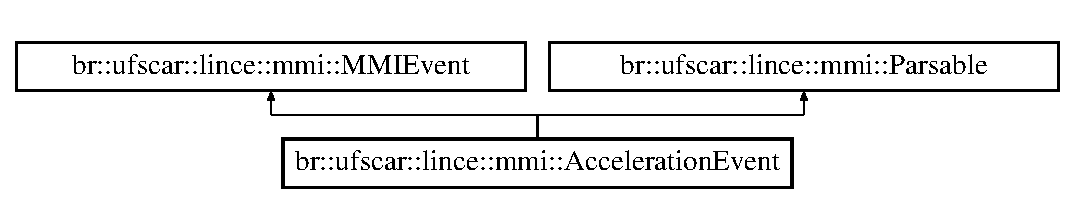
\includegraphics[height=2cm]{classbr_1_1ufscar_1_1lince_1_1mmi_1_1AccelerationEvent}
\end{center}
\end{figure}
\subsection*{Public Member Functions}
\begin{DoxyCompactItemize}
\item 
\hyperlink{classbr_1_1ufscar_1_1lince_1_1mmi_1_1AccelerationEvent_a0b697e055fc5bb1c3947435f0c25bd5d}{AccelerationEvent} (string deviceid, int \hyperlink{classbr_1_1ufscar_1_1lince_1_1mmi_1_1AccelerationEvent_aa8aa3708d87ebf38147a09b4d83eb604}{xValue}, int \hyperlink{classbr_1_1ufscar_1_1lince_1_1mmi_1_1AccelerationEvent_a1b87b4708c1f8ce65293b7fc3a148183}{yValue}, int \hyperlink{classbr_1_1ufscar_1_1lince_1_1mmi_1_1AccelerationEvent_a2fea6058c45c23e43ce8eb6f829a4990}{zValue})
\begin{DoxyCompactList}\small\item\em Construtor. \item\end{DoxyCompactList}\item 
virtual \hyperlink{classbr_1_1ufscar_1_1lince_1_1mmi_1_1AccelerationEvent_ab80cc047d3044e1450fb74bb1e62f8ab}{$\sim$AccelerationEvent} ()
\begin{DoxyCompactList}\small\item\em Destructor. \item\end{DoxyCompactList}\item 
virtual int \hyperlink{classbr_1_1ufscar_1_1lince_1_1mmi_1_1AccelerationEvent_a3e4798af9e022dbf7cdef27976437956}{getXValue} ()
\begin{DoxyCompactList}\small\item\em This method return the acceleration value of X axis. \item\end{DoxyCompactList}\item 
virtual int \hyperlink{classbr_1_1ufscar_1_1lince_1_1mmi_1_1AccelerationEvent_aa647428aca2ae84a2b9a58d5dd51ebb0}{getYValue} ()
\begin{DoxyCompactList}\small\item\em This method return the acceleration value of Y axis. \item\end{DoxyCompactList}\item 
virtual int \hyperlink{classbr_1_1ufscar_1_1lince_1_1mmi_1_1AccelerationEvent_a311a142a28339e32a09ba84971617351}{getZValue} ()
\begin{DoxyCompactList}\small\item\em This method return the acceleration value of Z axis. \item\end{DoxyCompactList}\end{DoxyCompactItemize}
\subsection*{Protected Member Functions}
\begin{DoxyCompactItemize}
\item 
\hyperlink{classbr_1_1ufscar_1_1lince_1_1mmi_1_1AccelerationEvent_aaf9298b6242c8894e04111a344add1fe}{AccelerationEvent} ()
\item 
void \hyperlink{classbr_1_1ufscar_1_1lince_1_1mmi_1_1AccelerationEvent_a5ad5b14f13e40450e619ce08e4ba9937}{parseXMLData} (\hyperlink{structbr_1_1ufscar_1_1lince_1_1mmi_1_1XMLData}{XMLData} $\ast$data)
\begin{DoxyCompactList}\small\item\em This methods realize the parse of a event represented by a XML Document. \item\end{DoxyCompactList}\end{DoxyCompactItemize}
\subsection*{Protected Attributes}
\begin{DoxyCompactItemize}
\item 
int \hyperlink{classbr_1_1ufscar_1_1lince_1_1mmi_1_1AccelerationEvent_aa8aa3708d87ebf38147a09b4d83eb604}{xValue}
\item 
int \hyperlink{classbr_1_1ufscar_1_1lince_1_1mmi_1_1AccelerationEvent_a1b87b4708c1f8ce65293b7fc3a148183}{yValue}
\item 
int \hyperlink{classbr_1_1ufscar_1_1lince_1_1mmi_1_1AccelerationEvent_a2fea6058c45c23e43ce8eb6f829a4990}{zValue}
\end{DoxyCompactItemize}
\subsection*{Friends}
\begin{DoxyCompactItemize}
\item 
class \hyperlink{classbr_1_1ufscar_1_1lince_1_1mmi_1_1AccelerationEvent_a5414bf6fb99d97af5a0b33c831e67026}{AccelerationFactory}
\end{DoxyCompactItemize}


\subsection{Constructor \& Destructor Documentation}
\hypertarget{classbr_1_1ufscar_1_1lince_1_1mmi_1_1AccelerationEvent_a0b697e055fc5bb1c3947435f0c25bd5d}{
\index{br::ufscar::lince::mmi::AccelerationEvent@{br::ufscar::lince::mmi::AccelerationEvent}!AccelerationEvent@{AccelerationEvent}}
\index{AccelerationEvent@{AccelerationEvent}!br::ufscar::lince::mmi::AccelerationEvent@{br::ufscar::lince::mmi::AccelerationEvent}}
\subsubsection[{AccelerationEvent}]{\setlength{\rightskip}{0pt plus 5cm}br::ufscar::lince::mmi::AccelerationEvent::AccelerationEvent (string {\em deviceid}, \/  int {\em xValue}, \/  int {\em yValue}, \/  int {\em zValue})}}
\label{classbr_1_1ufscar_1_1lince_1_1mmi_1_1AccelerationEvent_a0b697e055fc5bb1c3947435f0c25bd5d}


Construtor. 


\begin{DoxyParams}{Parameters}
\item[{\em deviceId}]The id of the device that generate the acceleration event. \item[{\em xValue}]The acceleration value of X axis. \item[{\em yValue}]The acceleration value of Y axis. \item[{\em zValue}]The acceleration value of Z axis. \end{DoxyParams}
\hypertarget{classbr_1_1ufscar_1_1lince_1_1mmi_1_1AccelerationEvent_ab80cc047d3044e1450fb74bb1e62f8ab}{
\index{br::ufscar::lince::mmi::AccelerationEvent@{br::ufscar::lince::mmi::AccelerationEvent}!$\sim$AccelerationEvent@{$\sim$AccelerationEvent}}
\index{$\sim$AccelerationEvent@{$\sim$AccelerationEvent}!br::ufscar::lince::mmi::AccelerationEvent@{br::ufscar::lince::mmi::AccelerationEvent}}
\subsubsection[{$\sim$AccelerationEvent}]{\setlength{\rightskip}{0pt plus 5cm}virtual br::ufscar::lince::mmi::AccelerationEvent::$\sim$AccelerationEvent ()\hspace{0.3cm}{\ttfamily  \mbox{[}virtual\mbox{]}}}}
\label{classbr_1_1ufscar_1_1lince_1_1mmi_1_1AccelerationEvent_ab80cc047d3044e1450fb74bb1e62f8ab}


Destructor. 

\hypertarget{classbr_1_1ufscar_1_1lince_1_1mmi_1_1AccelerationEvent_aaf9298b6242c8894e04111a344add1fe}{
\index{br::ufscar::lince::mmi::AccelerationEvent@{br::ufscar::lince::mmi::AccelerationEvent}!AccelerationEvent@{AccelerationEvent}}
\index{AccelerationEvent@{AccelerationEvent}!br::ufscar::lince::mmi::AccelerationEvent@{br::ufscar::lince::mmi::AccelerationEvent}}
\subsubsection[{AccelerationEvent}]{\setlength{\rightskip}{0pt plus 5cm}br::ufscar::lince::mmi::AccelerationEvent::AccelerationEvent ()\hspace{0.3cm}{\ttfamily  \mbox{[}protected\mbox{]}}}}
\label{classbr_1_1ufscar_1_1lince_1_1mmi_1_1AccelerationEvent_aaf9298b6242c8894e04111a344add1fe}


\subsection{Member Function Documentation}
\hypertarget{classbr_1_1ufscar_1_1lince_1_1mmi_1_1AccelerationEvent_a3e4798af9e022dbf7cdef27976437956}{
\index{br::ufscar::lince::mmi::AccelerationEvent@{br::ufscar::lince::mmi::AccelerationEvent}!getXValue@{getXValue}}
\index{getXValue@{getXValue}!br::ufscar::lince::mmi::AccelerationEvent@{br::ufscar::lince::mmi::AccelerationEvent}}
\subsubsection[{getXValue}]{\setlength{\rightskip}{0pt plus 5cm}virtual int br::ufscar::lince::mmi::AccelerationEvent::getXValue ()\hspace{0.3cm}{\ttfamily  \mbox{[}virtual\mbox{]}}}}
\label{classbr_1_1ufscar_1_1lince_1_1mmi_1_1AccelerationEvent_a3e4798af9e022dbf7cdef27976437956}


This method return the acceleration value of X axis. 

\begin{DoxyReturn}{Returns}
X axis Acceleration value of this Acceleration Event. 
\end{DoxyReturn}
\hypertarget{classbr_1_1ufscar_1_1lince_1_1mmi_1_1AccelerationEvent_aa647428aca2ae84a2b9a58d5dd51ebb0}{
\index{br::ufscar::lince::mmi::AccelerationEvent@{br::ufscar::lince::mmi::AccelerationEvent}!getYValue@{getYValue}}
\index{getYValue@{getYValue}!br::ufscar::lince::mmi::AccelerationEvent@{br::ufscar::lince::mmi::AccelerationEvent}}
\subsubsection[{getYValue}]{\setlength{\rightskip}{0pt plus 5cm}virtual int br::ufscar::lince::mmi::AccelerationEvent::getYValue ()\hspace{0.3cm}{\ttfamily  \mbox{[}virtual\mbox{]}}}}
\label{classbr_1_1ufscar_1_1lince_1_1mmi_1_1AccelerationEvent_aa647428aca2ae84a2b9a58d5dd51ebb0}


This method return the acceleration value of Y axis. 

\begin{DoxyReturn}{Returns}
Y axis Acceleration value of this Acceleration Event. 
\end{DoxyReturn}
\hypertarget{classbr_1_1ufscar_1_1lince_1_1mmi_1_1AccelerationEvent_a311a142a28339e32a09ba84971617351}{
\index{br::ufscar::lince::mmi::AccelerationEvent@{br::ufscar::lince::mmi::AccelerationEvent}!getZValue@{getZValue}}
\index{getZValue@{getZValue}!br::ufscar::lince::mmi::AccelerationEvent@{br::ufscar::lince::mmi::AccelerationEvent}}
\subsubsection[{getZValue}]{\setlength{\rightskip}{0pt plus 5cm}virtual int br::ufscar::lince::mmi::AccelerationEvent::getZValue ()\hspace{0.3cm}{\ttfamily  \mbox{[}virtual\mbox{]}}}}
\label{classbr_1_1ufscar_1_1lince_1_1mmi_1_1AccelerationEvent_a311a142a28339e32a09ba84971617351}


This method return the acceleration value of Z axis. 

\begin{DoxyReturn}{Returns}
Z axis Acceleration value of this Acceleration Event. 
\end{DoxyReturn}
\hypertarget{classbr_1_1ufscar_1_1lince_1_1mmi_1_1AccelerationEvent_a5ad5b14f13e40450e619ce08e4ba9937}{
\index{br::ufscar::lince::mmi::AccelerationEvent@{br::ufscar::lince::mmi::AccelerationEvent}!parseXMLData@{parseXMLData}}
\index{parseXMLData@{parseXMLData}!br::ufscar::lince::mmi::AccelerationEvent@{br::ufscar::lince::mmi::AccelerationEvent}}
\subsubsection[{parseXMLData}]{\setlength{\rightskip}{0pt plus 5cm}void br::ufscar::lince::mmi::AccelerationEvent::parseXMLData ({\bf XMLData} $\ast$ {\em data})\hspace{0.3cm}{\ttfamily  \mbox{[}protected, virtual\mbox{]}}}}
\label{classbr_1_1ufscar_1_1lince_1_1mmi_1_1AccelerationEvent_a5ad5b14f13e40450e619ce08e4ba9937}


This methods realize the parse of a event represented by a XML Document. 


\begin{DoxyParams}{Parameters}
\item[{\em data}]A instance of \hyperlink{structbr_1_1ufscar_1_1lince_1_1mmi_1_1XMLData}{XMLData} that contains the XML Document information. \end{DoxyParams}


Implements \hyperlink{classbr_1_1ufscar_1_1lince_1_1mmi_1_1Parsable_a6524a0a77abb3865e5d255e466b6159e}{br::ufscar::lince::mmi::Parsable}.



\subsection{Friends And Related Function Documentation}
\hypertarget{classbr_1_1ufscar_1_1lince_1_1mmi_1_1AccelerationEvent_a5414bf6fb99d97af5a0b33c831e67026}{
\index{br::ufscar::lince::mmi::AccelerationEvent@{br::ufscar::lince::mmi::AccelerationEvent}!AccelerationFactory@{AccelerationFactory}}
\index{AccelerationFactory@{AccelerationFactory}!br::ufscar::lince::mmi::AccelerationEvent@{br::ufscar::lince::mmi::AccelerationEvent}}
\subsubsection[{AccelerationFactory}]{\setlength{\rightskip}{0pt plus 5cm}friend class {\bf AccelerationFactory}\hspace{0.3cm}{\ttfamily  \mbox{[}friend\mbox{]}}}}
\label{classbr_1_1ufscar_1_1lince_1_1mmi_1_1AccelerationEvent_a5414bf6fb99d97af5a0b33c831e67026}


\subsection{Field Documentation}
\hypertarget{classbr_1_1ufscar_1_1lince_1_1mmi_1_1AccelerationEvent_aa8aa3708d87ebf38147a09b4d83eb604}{
\index{br::ufscar::lince::mmi::AccelerationEvent@{br::ufscar::lince::mmi::AccelerationEvent}!xValue@{xValue}}
\index{xValue@{xValue}!br::ufscar::lince::mmi::AccelerationEvent@{br::ufscar::lince::mmi::AccelerationEvent}}
\subsubsection[{xValue}]{\setlength{\rightskip}{0pt plus 5cm}int {\bf br::ufscar::lince::mmi::AccelerationEvent::xValue}\hspace{0.3cm}{\ttfamily  \mbox{[}protected\mbox{]}}}}
\label{classbr_1_1ufscar_1_1lince_1_1mmi_1_1AccelerationEvent_aa8aa3708d87ebf38147a09b4d83eb604}
\hypertarget{classbr_1_1ufscar_1_1lince_1_1mmi_1_1AccelerationEvent_a1b87b4708c1f8ce65293b7fc3a148183}{
\index{br::ufscar::lince::mmi::AccelerationEvent@{br::ufscar::lince::mmi::AccelerationEvent}!yValue@{yValue}}
\index{yValue@{yValue}!br::ufscar::lince::mmi::AccelerationEvent@{br::ufscar::lince::mmi::AccelerationEvent}}
\subsubsection[{yValue}]{\setlength{\rightskip}{0pt plus 5cm}int {\bf br::ufscar::lince::mmi::AccelerationEvent::yValue}\hspace{0.3cm}{\ttfamily  \mbox{[}protected\mbox{]}}}}
\label{classbr_1_1ufscar_1_1lince_1_1mmi_1_1AccelerationEvent_a1b87b4708c1f8ce65293b7fc3a148183}
\hypertarget{classbr_1_1ufscar_1_1lince_1_1mmi_1_1AccelerationEvent_a2fea6058c45c23e43ce8eb6f829a4990}{
\index{br::ufscar::lince::mmi::AccelerationEvent@{br::ufscar::lince::mmi::AccelerationEvent}!zValue@{zValue}}
\index{zValue@{zValue}!br::ufscar::lince::mmi::AccelerationEvent@{br::ufscar::lince::mmi::AccelerationEvent}}
\subsubsection[{zValue}]{\setlength{\rightskip}{0pt plus 5cm}int {\bf br::ufscar::lince::mmi::AccelerationEvent::zValue}\hspace{0.3cm}{\ttfamily  \mbox{[}protected\mbox{]}}}}
\label{classbr_1_1ufscar_1_1lince_1_1mmi_1_1AccelerationEvent_a2fea6058c45c23e43ce8eb6f829a4990}


The documentation for this class was generated from the following file:\begin{DoxyCompactItemize}
\item 
include/\hyperlink{AccelerationEvent_8h}{AccelerationEvent.h}\end{DoxyCompactItemize}

\hypertarget{classbr_1_1ufscar_1_1lince_1_1mmi_1_1AccelerationFactory}{
\section{br::ufscar::lince::mmi::AccelerationFactory Class Reference}
\label{classbr_1_1ufscar_1_1lince_1_1mmi_1_1AccelerationFactory}\index{br::ufscar::lince::mmi::AccelerationFactory@{br::ufscar::lince::mmi::AccelerationFactory}}
}


{\ttfamily \#include $<$AccelerationFactory.h$>$}

Inheritance diagram for br::ufscar::lince::mmi::AccelerationFactory:\begin{figure}[H]
\begin{center}
\leavevmode
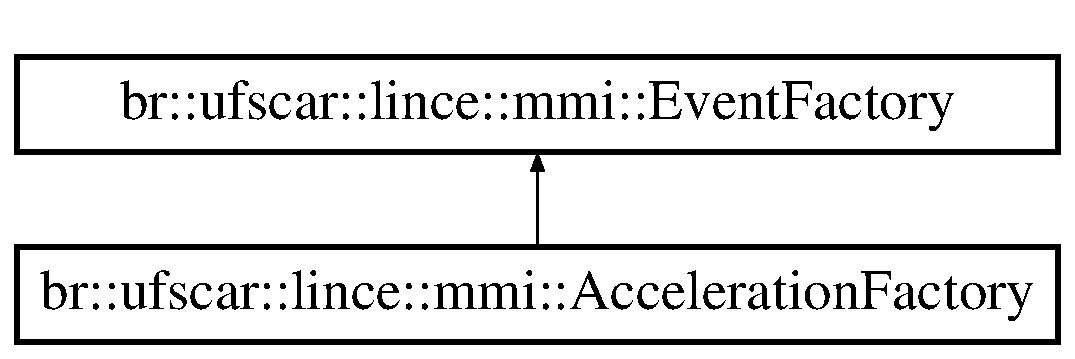
\includegraphics[height=2cm]{classbr_1_1ufscar_1_1lince_1_1mmi_1_1AccelerationFactory}
\end{center}
\end{figure}
\subsection*{Public Member Functions}
\begin{DoxyCompactItemize}
\item 
\hyperlink{classbr_1_1ufscar_1_1lince_1_1mmi_1_1AccelerationFactory_aeba6ded86331f14a169b9e507a0e6531}{AccelerationFactory} ()
\item 
virtual \hyperlink{classbr_1_1ufscar_1_1lince_1_1mmi_1_1AccelerationFactory_a5df5c784ea0f38f5adbd54a213bb0852}{$\sim$AccelerationFactory} ()
\item 
virtual \hyperlink{classbr_1_1ufscar_1_1lince_1_1mmi_1_1MMIEvent}{MMIEvent} $\ast$ \hyperlink{classbr_1_1ufscar_1_1lince_1_1mmi_1_1AccelerationFactory_a5b8858d27f1b956b6c1f27648c010d74}{CreateEvent} (\hyperlink{structbr_1_1ufscar_1_1lince_1_1mmi_1_1XMLData}{XMLData} $\ast$data)
\end{DoxyCompactItemize}


\subsection{Constructor \& Destructor Documentation}
\hypertarget{classbr_1_1ufscar_1_1lince_1_1mmi_1_1AccelerationFactory_aeba6ded86331f14a169b9e507a0e6531}{
\index{br::ufscar::lince::mmi::AccelerationFactory@{br::ufscar::lince::mmi::AccelerationFactory}!AccelerationFactory@{AccelerationFactory}}
\index{AccelerationFactory@{AccelerationFactory}!br::ufscar::lince::mmi::AccelerationFactory@{br::ufscar::lince::mmi::AccelerationFactory}}
\subsubsection[{AccelerationFactory}]{\setlength{\rightskip}{0pt plus 5cm}br::ufscar::lince::mmi::AccelerationFactory::AccelerationFactory ()}}
\label{classbr_1_1ufscar_1_1lince_1_1mmi_1_1AccelerationFactory_aeba6ded86331f14a169b9e507a0e6531}
\hypertarget{classbr_1_1ufscar_1_1lince_1_1mmi_1_1AccelerationFactory_a5df5c784ea0f38f5adbd54a213bb0852}{
\index{br::ufscar::lince::mmi::AccelerationFactory@{br::ufscar::lince::mmi::AccelerationFactory}!$\sim$AccelerationFactory@{$\sim$AccelerationFactory}}
\index{$\sim$AccelerationFactory@{$\sim$AccelerationFactory}!br::ufscar::lince::mmi::AccelerationFactory@{br::ufscar::lince::mmi::AccelerationFactory}}
\subsubsection[{$\sim$AccelerationFactory}]{\setlength{\rightskip}{0pt plus 5cm}virtual br::ufscar::lince::mmi::AccelerationFactory::$\sim$AccelerationFactory ()\hspace{0.3cm}{\ttfamily  \mbox{[}virtual\mbox{]}}}}
\label{classbr_1_1ufscar_1_1lince_1_1mmi_1_1AccelerationFactory_a5df5c784ea0f38f5adbd54a213bb0852}


\subsection{Member Function Documentation}
\hypertarget{classbr_1_1ufscar_1_1lince_1_1mmi_1_1AccelerationFactory_a5b8858d27f1b956b6c1f27648c010d74}{
\index{br::ufscar::lince::mmi::AccelerationFactory@{br::ufscar::lince::mmi::AccelerationFactory}!CreateEvent@{CreateEvent}}
\index{CreateEvent@{CreateEvent}!br::ufscar::lince::mmi::AccelerationFactory@{br::ufscar::lince::mmi::AccelerationFactory}}
\subsubsection[{CreateEvent}]{\setlength{\rightskip}{0pt plus 5cm}virtual {\bf MMIEvent}$\ast$ br::ufscar::lince::mmi::AccelerationFactory::CreateEvent ({\bf XMLData} $\ast$ {\em data})\hspace{0.3cm}{\ttfamily  \mbox{[}virtual\mbox{]}}}}
\label{classbr_1_1ufscar_1_1lince_1_1mmi_1_1AccelerationFactory_a5b8858d27f1b956b6c1f27648c010d74}


Implements \hyperlink{classbr_1_1ufscar_1_1lince_1_1mmi_1_1EventFactory_a19ad2165726a29a55c921f569764290b}{br::ufscar::lince::mmi::EventFactory}.



The documentation for this class was generated from the following file:\begin{DoxyCompactItemize}
\item 
include/\hyperlink{AccelerationFactory_8h}{AccelerationFactory.h}\end{DoxyCompactItemize}

\hypertarget{classbr_1_1ufscar_1_1lince_1_1xpta_1_1mmi_1_1inkmllib_1_1Channel}{
\section{br::ufscar::lince::xpta::mmi::inkmllib::Channel Class Reference}
\label{classbr_1_1ufscar_1_1lince_1_1xpta_1_1mmi_1_1inkmllib_1_1Channel}\index{br::ufscar::lince::xpta::mmi::inkmllib::Channel@{br::ufscar::lince::xpta::mmi::inkmllib::Channel}}
}


Classe que representa um channel de um InkML, responsável por descrever os dados que podem estar codificados em um trace.  




{\ttfamily \#include $<$Channel.h$>$}

\subsection*{Public Member Functions}
\begin{DoxyCompactItemize}
\item 
\hyperlink{classbr_1_1ufscar_1_1lince_1_1xpta_1_1mmi_1_1inkmllib_1_1Channel_a8caba3ff1f520d271fddce9dcc75f7a4}{Channel} (char $\ast$\hyperlink{classbr_1_1ufscar_1_1lince_1_1xpta_1_1mmi_1_1inkmllib_1_1Channel_afb61ee0d3d7834733557c09adf3b6bcb}{name}, long \hyperlink{classbr_1_1ufscar_1_1lince_1_1xpta_1_1mmi_1_1inkmllib_1_1Channel_ac0ca63bd45cff57bd599ea6a74c3e205}{min}, long \hyperlink{classbr_1_1ufscar_1_1lince_1_1xpta_1_1mmi_1_1inkmllib_1_1Channel_a026225dffda8f84b452db591226cee12}{max}, char $\ast$\hyperlink{classbr_1_1ufscar_1_1lince_1_1xpta_1_1mmi_1_1inkmllib_1_1Channel_ade05efe4076717c540529d5b82c81183}{units})
\begin{DoxyCompactList}\small\item\em Cria um channel. \item\end{DoxyCompactList}\item 
\hyperlink{classbr_1_1ufscar_1_1lince_1_1xpta_1_1mmi_1_1inkmllib_1_1Channel_a779790d4eabe0735325b8eb5d9139fff}{Channel} (char $\ast$\hyperlink{classbr_1_1ufscar_1_1lince_1_1xpta_1_1mmi_1_1inkmllib_1_1Channel_afb61ee0d3d7834733557c09adf3b6bcb}{name}, long \hyperlink{classbr_1_1ufscar_1_1lince_1_1xpta_1_1mmi_1_1inkmllib_1_1Channel_ac0ca63bd45cff57bd599ea6a74c3e205}{min}, long \hyperlink{classbr_1_1ufscar_1_1lince_1_1xpta_1_1mmi_1_1inkmllib_1_1Channel_a026225dffda8f84b452db591226cee12}{max}, \hyperlink{namespacebr_1_1ufscar_1_1lince_1_1xpta_1_1mmi_1_1inkmllib_aa20053e417f8d2a79fcdc702e3e23673}{INKML\_\-UNITS} \hyperlink{classbr_1_1ufscar_1_1lince_1_1xpta_1_1mmi_1_1inkmllib_1_1Channel_ade05efe4076717c540529d5b82c81183}{units})
\begin{DoxyCompactList}\small\item\em Cria um channel. \item\end{DoxyCompactList}\item 
\hyperlink{classbr_1_1ufscar_1_1lince_1_1xpta_1_1mmi_1_1inkmllib_1_1Channel_a64137ab8133b3235bc89ab446a94daab}{Channel} (char $\ast$\hyperlink{classbr_1_1ufscar_1_1lince_1_1xpta_1_1mmi_1_1inkmllib_1_1Channel_afb61ee0d3d7834733557c09adf3b6bcb}{name})
\begin{DoxyCompactList}\small\item\em Cria um channel. \item\end{DoxyCompactList}\item 
\hyperlink{namespacebr_1_1ufscar_1_1lince_1_1xpta_1_1mmi_1_1inkmllib_aa20053e417f8d2a79fcdc702e3e23673}{INKML\_\-UNITS} \hyperlink{classbr_1_1ufscar_1_1lince_1_1xpta_1_1mmi_1_1inkmllib_1_1Channel_a961e5ef52b4db4b48ddd1a31441afa37}{getUnit} ()
\begin{DoxyCompactList}\small\item\em Retorna a unidade em que os valores do channel estão expressos. \item\end{DoxyCompactList}\item 
char $\ast$ \hyperlink{classbr_1_1ufscar_1_1lince_1_1xpta_1_1mmi_1_1inkmllib_1_1Channel_a0c8bc29ec3a0bed2c1edcb2a142e3e8d}{getName} ()
\begin{DoxyCompactList}\small\item\em Retorna o nome do channel. \item\end{DoxyCompactList}\end{DoxyCompactItemize}
\subsection*{Data Fields}
\begin{DoxyCompactItemize}
\item 
char $\ast$ \hyperlink{classbr_1_1ufscar_1_1lince_1_1xpta_1_1mmi_1_1inkmllib_1_1Channel_afb61ee0d3d7834733557c09adf3b6bcb}{name}
\begin{DoxyCompactList}\small\item\em to store the 'name' attribute value. It is a mandatory field. \item\end{DoxyCompactList}\item 
long \hyperlink{classbr_1_1ufscar_1_1lince_1_1xpta_1_1mmi_1_1inkmllib_1_1Channel_ac0ca63bd45cff57bd599ea6a74c3e205}{min}
\begin{DoxyCompactList}\small\item\em to store the 'min' attribute value. \item\end{DoxyCompactList}\item 
long \hyperlink{classbr_1_1ufscar_1_1lince_1_1xpta_1_1mmi_1_1inkmllib_1_1Channel_a026225dffda8f84b452db591226cee12}{max}
\begin{DoxyCompactList}\small\item\em to store the 'max' attribute value. \item\end{DoxyCompactList}\item 
\hyperlink{namespacebr_1_1ufscar_1_1lince_1_1xpta_1_1mmi_1_1inkmllib_aa20053e417f8d2a79fcdc702e3e23673}{INKML\_\-UNITS} \hyperlink{classbr_1_1ufscar_1_1lince_1_1xpta_1_1mmi_1_1inkmllib_1_1Channel_ade05efe4076717c540529d5b82c81183}{units}
\begin{DoxyCompactList}\small\item\em If value not given for min and/or max then the channel value is unbounded in either direction to store the 'units' attribute value. \item\end{DoxyCompactList}\end{DoxyCompactItemize}


\subsection{Detailed Description}
Classe que representa um channel de um InkML, responsável por descrever os dados que podem estar codificados em um trace. Mais informações em \href{http://sourceforge.net/apps/trac/inkmltk/wiki/InkMLLib}{\tt http://sourceforge.net/apps/trac/inkmltk/wiki/InkMLLib} 

\subsection{Constructor \& Destructor Documentation}
\hypertarget{classbr_1_1ufscar_1_1lince_1_1xpta_1_1mmi_1_1inkmllib_1_1Channel_a8caba3ff1f520d271fddce9dcc75f7a4}{
\index{br::ufscar::lince::xpta::mmi::inkmllib::Channel@{br::ufscar::lince::xpta::mmi::inkmllib::Channel}!Channel@{Channel}}
\index{Channel@{Channel}!br::ufscar::lince::xpta::mmi::inkmllib::Channel@{br::ufscar::lince::xpta::mmi::inkmllib::Channel}}
\subsubsection[{Channel}]{\setlength{\rightskip}{0pt plus 5cm}br::ufscar::lince::xpta::mmi::inkmllib::Channel::Channel (char $\ast$ {\em name}, \/  long {\em min}, \/  long {\em max}, \/  char $\ast$ {\em units})}}
\label{classbr_1_1ufscar_1_1lince_1_1xpta_1_1mmi_1_1inkmllib_1_1Channel_a8caba3ff1f520d271fddce9dcc75f7a4}


Cria um channel. 


\begin{DoxyParams}{Parameters}
\item[{\em name}]Nome do channel. \item[{\em min}]Limite inferior para os valores do channel \item[{\em max}]Limite superior para os valores do channel \item[{\em units}]Unidade em quem os valores do channel estão expressos. \end{DoxyParams}
\hypertarget{classbr_1_1ufscar_1_1lince_1_1xpta_1_1mmi_1_1inkmllib_1_1Channel_a779790d4eabe0735325b8eb5d9139fff}{
\index{br::ufscar::lince::xpta::mmi::inkmllib::Channel@{br::ufscar::lince::xpta::mmi::inkmllib::Channel}!Channel@{Channel}}
\index{Channel@{Channel}!br::ufscar::lince::xpta::mmi::inkmllib::Channel@{br::ufscar::lince::xpta::mmi::inkmllib::Channel}}
\subsubsection[{Channel}]{\setlength{\rightskip}{0pt plus 5cm}br::ufscar::lince::xpta::mmi::inkmllib::Channel::Channel (char $\ast$ {\em name}, \/  long {\em min}, \/  long {\em max}, \/  {\bf INKML\_\-UNITS} {\em units})}}
\label{classbr_1_1ufscar_1_1lince_1_1xpta_1_1mmi_1_1inkmllib_1_1Channel_a779790d4eabe0735325b8eb5d9139fff}


Cria um channel. 


\begin{DoxyParams}{Parameters}
\item[{\em name}]Nome do channel. \item[{\em min}]Limite inferior para os valores do channel \item[{\em max}]Limite superior para os valores do channel \item[{\em units}]Unidade em quem os valores do channel estão expressos. \end{DoxyParams}
\hypertarget{classbr_1_1ufscar_1_1lince_1_1xpta_1_1mmi_1_1inkmllib_1_1Channel_a64137ab8133b3235bc89ab446a94daab}{
\index{br::ufscar::lince::xpta::mmi::inkmllib::Channel@{br::ufscar::lince::xpta::mmi::inkmllib::Channel}!Channel@{Channel}}
\index{Channel@{Channel}!br::ufscar::lince::xpta::mmi::inkmllib::Channel@{br::ufscar::lince::xpta::mmi::inkmllib::Channel}}
\subsubsection[{Channel}]{\setlength{\rightskip}{0pt plus 5cm}br::ufscar::lince::xpta::mmi::inkmllib::Channel::Channel (char $\ast$ {\em name})}}
\label{classbr_1_1ufscar_1_1lince_1_1xpta_1_1mmi_1_1inkmllib_1_1Channel_a64137ab8133b3235bc89ab446a94daab}


Cria um channel. 


\begin{DoxyParams}{Parameters}
\item[{\em name}]Nome do channel. \end{DoxyParams}


\subsection{Member Function Documentation}
\hypertarget{classbr_1_1ufscar_1_1lince_1_1xpta_1_1mmi_1_1inkmllib_1_1Channel_a0c8bc29ec3a0bed2c1edcb2a142e3e8d}{
\index{br::ufscar::lince::xpta::mmi::inkmllib::Channel@{br::ufscar::lince::xpta::mmi::inkmllib::Channel}!getName@{getName}}
\index{getName@{getName}!br::ufscar::lince::xpta::mmi::inkmllib::Channel@{br::ufscar::lince::xpta::mmi::inkmllib::Channel}}
\subsubsection[{getName}]{\setlength{\rightskip}{0pt plus 5cm}char$\ast$ br::ufscar::lince::xpta::mmi::inkmllib::Channel::getName ()\hspace{0.3cm}{\ttfamily  \mbox{[}inline\mbox{]}}}}
\label{classbr_1_1ufscar_1_1lince_1_1xpta_1_1mmi_1_1inkmllib_1_1Channel_a0c8bc29ec3a0bed2c1edcb2a142e3e8d}


Retorna o nome do channel. 

\begin{DoxyReturn}{Returns}
O nome 
\end{DoxyReturn}
\hypertarget{classbr_1_1ufscar_1_1lince_1_1xpta_1_1mmi_1_1inkmllib_1_1Channel_a961e5ef52b4db4b48ddd1a31441afa37}{
\index{br::ufscar::lince::xpta::mmi::inkmllib::Channel@{br::ufscar::lince::xpta::mmi::inkmllib::Channel}!getUnit@{getUnit}}
\index{getUnit@{getUnit}!br::ufscar::lince::xpta::mmi::inkmllib::Channel@{br::ufscar::lince::xpta::mmi::inkmllib::Channel}}
\subsubsection[{getUnit}]{\setlength{\rightskip}{0pt plus 5cm}{\bf INKML\_\-UNITS} br::ufscar::lince::xpta::mmi::inkmllib::Channel::getUnit ()\hspace{0.3cm}{\ttfamily  \mbox{[}inline\mbox{]}}}}
\label{classbr_1_1ufscar_1_1lince_1_1xpta_1_1mmi_1_1inkmllib_1_1Channel_a961e5ef52b4db4b48ddd1a31441afa37}


Retorna a unidade em que os valores do channel estão expressos. 

\begin{DoxyReturn}{Returns}
A unidade 
\end{DoxyReturn}


\subsection{Field Documentation}
\hypertarget{classbr_1_1ufscar_1_1lince_1_1xpta_1_1mmi_1_1inkmllib_1_1Channel_a026225dffda8f84b452db591226cee12}{
\index{br::ufscar::lince::xpta::mmi::inkmllib::Channel@{br::ufscar::lince::xpta::mmi::inkmllib::Channel}!max@{max}}
\index{max@{max}!br::ufscar::lince::xpta::mmi::inkmllib::Channel@{br::ufscar::lince::xpta::mmi::inkmllib::Channel}}
\subsubsection[{max}]{\setlength{\rightskip}{0pt plus 5cm}long {\bf br::ufscar::lince::xpta::mmi::inkmllib::Channel::max}}}
\label{classbr_1_1ufscar_1_1lince_1_1xpta_1_1mmi_1_1inkmllib_1_1Channel_a026225dffda8f84b452db591226cee12}


to store the 'max' attribute value. 

It gives the max range of channel data value. \hypertarget{classbr_1_1ufscar_1_1lince_1_1xpta_1_1mmi_1_1inkmllib_1_1Channel_ac0ca63bd45cff57bd599ea6a74c3e205}{
\index{br::ufscar::lince::xpta::mmi::inkmllib::Channel@{br::ufscar::lince::xpta::mmi::inkmllib::Channel}!min@{min}}
\index{min@{min}!br::ufscar::lince::xpta::mmi::inkmllib::Channel@{br::ufscar::lince::xpta::mmi::inkmllib::Channel}}
\subsubsection[{min}]{\setlength{\rightskip}{0pt plus 5cm}long {\bf br::ufscar::lince::xpta::mmi::inkmllib::Channel::min}}}
\label{classbr_1_1ufscar_1_1lince_1_1xpta_1_1mmi_1_1inkmllib_1_1Channel_ac0ca63bd45cff57bd599ea6a74c3e205}


to store the 'min' attribute value. 

It gives the min range of channel data value. \hypertarget{classbr_1_1ufscar_1_1lince_1_1xpta_1_1mmi_1_1inkmllib_1_1Channel_afb61ee0d3d7834733557c09adf3b6bcb}{
\index{br::ufscar::lince::xpta::mmi::inkmllib::Channel@{br::ufscar::lince::xpta::mmi::inkmllib::Channel}!name@{name}}
\index{name@{name}!br::ufscar::lince::xpta::mmi::inkmllib::Channel@{br::ufscar::lince::xpta::mmi::inkmllib::Channel}}
\subsubsection[{name}]{\setlength{\rightskip}{0pt plus 5cm}char$\ast$ {\bf br::ufscar::lince::xpta::mmi::inkmllib::Channel::name}}}
\label{classbr_1_1ufscar_1_1lince_1_1xpta_1_1mmi_1_1inkmllib_1_1Channel_afb61ee0d3d7834733557c09adf3b6bcb}


to store the 'name' attribute value. It is a mandatory field. 

\hypertarget{classbr_1_1ufscar_1_1lince_1_1xpta_1_1mmi_1_1inkmllib_1_1Channel_ade05efe4076717c540529d5b82c81183}{
\index{br::ufscar::lince::xpta::mmi::inkmllib::Channel@{br::ufscar::lince::xpta::mmi::inkmllib::Channel}!units@{units}}
\index{units@{units}!br::ufscar::lince::xpta::mmi::inkmllib::Channel@{br::ufscar::lince::xpta::mmi::inkmllib::Channel}}
\subsubsection[{units}]{\setlength{\rightskip}{0pt plus 5cm}{\bf INKML\_\-UNITS} {\bf br::ufscar::lince::xpta::mmi::inkmllib::Channel::units}}}
\label{classbr_1_1ufscar_1_1lince_1_1xpta_1_1mmi_1_1inkmllib_1_1Channel_ade05efe4076717c540529d5b82c81183}


If value not given for min and/or max then the channel value is unbounded in either direction to store the 'units' attribute value. 



The documentation for this class was generated from the following file:\begin{DoxyCompactItemize}
\item 
include/ink/\hyperlink{Channel_8h}{Channel.h}\end{DoxyCompactItemize}

\hypertarget{classbr_1_1ufscar_1_1lince_1_1mmi_1_1zeroconf_1_1CommunicationManager}{
\section{br::ufscar::lince::mmi::zeroconf::CommunicationManager Class Reference}
\label{classbr_1_1ufscar_1_1lince_1_1mmi_1_1zeroconf_1_1CommunicationManager}\index{br::ufscar::lince::mmi::zeroconf::CommunicationManager@{br::ufscar::lince::mmi::zeroconf::CommunicationManager}}
}


Classe responsável pelo recebimento via rede, usando o protocolo ZeroConf, de mensagens XML representando eventos multimodais.  




{\ttfamily \#include $<$CommunicationManager.h$>$}

Inheritance diagram for br::ufscar::lince::mmi::zeroconf::CommunicationManager:\begin{figure}[H]
\begin{center}
\leavevmode
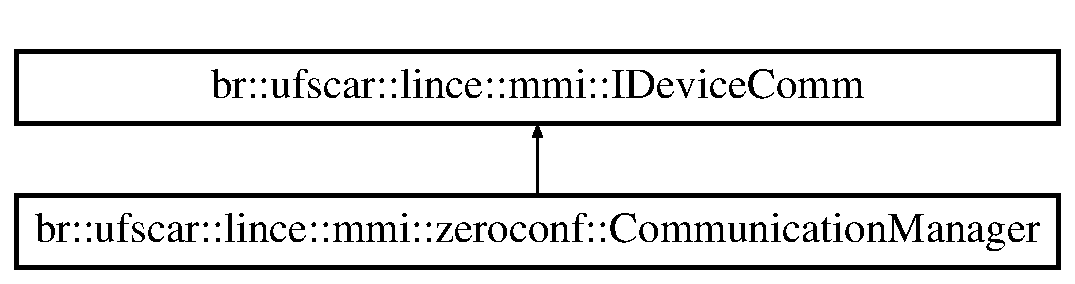
\includegraphics[height=2cm]{classbr_1_1ufscar_1_1lince_1_1mmi_1_1zeroconf_1_1CommunicationManager}
\end{center}
\end{figure}
\subsection*{Public Member Functions}
\begin{DoxyCompactItemize}
\item 
virtual void \hyperlink{classbr_1_1ufscar_1_1lince_1_1mmi_1_1zeroconf_1_1CommunicationManager_a580a75f652a1b1e233b6075f740555e1}{connect} ()
\begin{DoxyCompactList}\small\item\em This method stabilishes a connect between the device and the \hyperlink{classbr_1_1ufscar_1_1lince_1_1mmi_1_1MMIManager}{MMIManager}, allowing the device reports his multimodal events. \item\end{DoxyCompactList}\item 
virtual void \hyperlink{classbr_1_1ufscar_1_1lince_1_1mmi_1_1zeroconf_1_1CommunicationManager_a1c41c5541bf5c02b78f3dc10a045c7f6}{disconnect} ()
\begin{DoxyCompactList}\small\item\em This method finishes the connection between the devica and \hyperlink{classbr_1_1ufscar_1_1lince_1_1mmi_1_1MMIManager}{MMIManager}. \item\end{DoxyCompactList}\item 
virtual void \hyperlink{classbr_1_1ufscar_1_1lince_1_1mmi_1_1zeroconf_1_1CommunicationManager_a40b30969966a6517d21cf9a1cf5c3da8}{sendToDevice} (vector$<$ string $>$ $\ast$args)
\begin{DoxyCompactList}\small\item\em This method allows send a message to the device. \item\end{DoxyCompactList}\item 
virtual string \hyperlink{classbr_1_1ufscar_1_1lince_1_1mmi_1_1zeroconf_1_1CommunicationManager_ac81ba73dafe9e2ca558fad5d46f09e8c}{getDeviceId} ()
\begin{DoxyCompactList}\small\item\em This method return the id of the device. \item\end{DoxyCompactList}\item 
virtual void \hyperlink{classbr_1_1ufscar_1_1lince_1_1mmi_1_1zeroconf_1_1CommunicationManager_aef7bfab9cd63ab8e75fb0782e019574b}{release} ()
\begin{DoxyCompactList}\small\item\em This method make the device reset its internals variables. \item\end{DoxyCompactList}\item 
virtual void \hyperlink{classbr_1_1ufscar_1_1lince_1_1mmi_1_1zeroconf_1_1CommunicationManager_a3f1607eb5807f50ee40882543220d0fb}{run} ()
\begin{DoxyCompactList}\small\item\em Laço infinito em que dados representando um evento são esperados. \item\end{DoxyCompactList}\item 
int \hyperlink{classbr_1_1ufscar_1_1lince_1_1mmi_1_1zeroconf_1_1CommunicationManager_ae914529050d209469d98e2f03e42ce85}{startSocket} ()
\begin{DoxyCompactList}\small\item\em Inicializa um socket e espera por conexões de dispositivos externos. \item\end{DoxyCompactList}\item 
void \hyperlink{classbr_1_1ufscar_1_1lince_1_1mmi_1_1zeroconf_1_1CommunicationManager_a9255db8e4fc96b6cd99b3ba67c4e79e5}{createServices} (AvahiClient $\ast$c)
\begin{DoxyCompactList}\small\item\em Só é chamada \char`\"{}internamente\char`\"{}, mas não pode ser protected porque é chamada pelas funções de callback, que não pertencem a classe. \item\end{DoxyCompactList}\end{DoxyCompactItemize}
\subsection*{Static Public Member Functions}
\begin{DoxyCompactItemize}
\item 
static \hyperlink{classbr_1_1ufscar_1_1lince_1_1mmi_1_1zeroconf_1_1CommunicationManager}{CommunicationManager} $\ast$ \hyperlink{classbr_1_1ufscar_1_1lince_1_1mmi_1_1zeroconf_1_1CommunicationManager_ae9d111bd7e4f269a80deee7bbe9c9fcd}{getInstance} ()
\begin{DoxyCompactList}\small\item\em Acessa a instância única. \item\end{DoxyCompactList}\item 
static void \hyperlink{classbr_1_1ufscar_1_1lince_1_1mmi_1_1zeroconf_1_1CommunicationManager_ac7e195d0638ae6794150c9efb146259c}{clientCallback} (AvahiClient $\ast$c, AvahiClientState state, AVAHI\_\-GCC\_\-UNUSED void $\ast$userdata)
\begin{DoxyCompactList}\small\item\em TODO Comentar. \item\end{DoxyCompactList}\item 
static void \hyperlink{classbr_1_1ufscar_1_1lince_1_1mmi_1_1zeroconf_1_1CommunicationManager_a53b4fbff9b68d1c90d2b6f9da2ec7da9}{entryGroupCallback} (AvahiEntryGroup $\ast$g, AvahiEntryGroupState state, AVAHI\_\-GCC\_\-UNUSED void $\ast$userdata)
\begin{DoxyCompactList}\small\item\em TODO Comentar. \item\end{DoxyCompactList}\end{DoxyCompactItemize}
\subsection*{Protected Member Functions}
\begin{DoxyCompactItemize}
\item 
\hyperlink{classbr_1_1ufscar_1_1lince_1_1mmi_1_1zeroconf_1_1CommunicationManager_a4bb343041bd8a27f7640a3a0405459f7}{CommunicationManager} ()
\begin{DoxyCompactList}\small\item\em Constrói a instância única. \item\end{DoxyCompactList}\item 
\hyperlink{classbr_1_1ufscar_1_1lince_1_1mmi_1_1zeroconf_1_1CommunicationManager_adc5185400454d122aa325f2e79017eba}{$\sim$CommunicationManager} ()
\begin{DoxyCompactList}\small\item\em Destrói o \hyperlink{classbr_1_1ufscar_1_1lince_1_1mmi_1_1zeroconf_1_1CommunicationManager}{CommunicationManager}. \item\end{DoxyCompactList}\end{DoxyCompactItemize}
\subsection*{Protected Attributes}
\begin{DoxyCompactItemize}
\item 
HLoggerPtr \hyperlink{classbr_1_1ufscar_1_1lince_1_1mmi_1_1zeroconf_1_1CommunicationManager_aca59ba5611ac71c96c668a6bad73405a}{logger}
\begin{DoxyCompactList}\small\item\em Responsável pelo controle das mensagens de log. \item\end{DoxyCompactList}\item 
AvahiEntryGroup $\ast$ \hyperlink{classbr_1_1ufscar_1_1lince_1_1mmi_1_1zeroconf_1_1CommunicationManager_a45a446d4698e5e9de6faa0f7c36e5af7}{group}
\begin{DoxyCompactList}\small\item\em TODO Comentar. \item\end{DoxyCompactList}\item 
AvahiSimplePoll $\ast$ \hyperlink{classbr_1_1ufscar_1_1lince_1_1mmi_1_1zeroconf_1_1CommunicationManager_abe4f838b42e69ac6c597c9e83a2962ff}{simplePoll}
\begin{DoxyCompactList}\small\item\em TODO Comentar. \item\end{DoxyCompactList}\item 
char $\ast$ \hyperlink{classbr_1_1ufscar_1_1lince_1_1mmi_1_1zeroconf_1_1CommunicationManager_aed1f1d17b6d93eee2a4b31db0530e9dd}{name}
\begin{DoxyCompactList}\small\item\em TODO Comentar. \item\end{DoxyCompactList}\end{DoxyCompactItemize}
\subsection*{Static Protected Attributes}
\begin{DoxyCompactItemize}
\item 
static \hyperlink{classbr_1_1ufscar_1_1lince_1_1mmi_1_1zeroconf_1_1CommunicationManager}{CommunicationManager} $\ast$ \hyperlink{classbr_1_1ufscar_1_1lince_1_1mmi_1_1zeroconf_1_1CommunicationManager_a661f79b7946162c5954531547e41c619}{\_\-instance}
\begin{DoxyCompactList}\small\item\em Instância única. \item\end{DoxyCompactList}\end{DoxyCompactItemize}


\subsection{Detailed Description}
Classe responsável pelo recebimento via rede, usando o protocolo ZeroConf, de mensagens XML representando eventos multimodais. 

\subsection{Constructor \& Destructor Documentation}
\hypertarget{classbr_1_1ufscar_1_1lince_1_1mmi_1_1zeroconf_1_1CommunicationManager_a4bb343041bd8a27f7640a3a0405459f7}{
\index{br::ufscar::lince::mmi::zeroconf::CommunicationManager@{br::ufscar::lince::mmi::zeroconf::CommunicationManager}!CommunicationManager@{CommunicationManager}}
\index{CommunicationManager@{CommunicationManager}!br::ufscar::lince::mmi::zeroconf::CommunicationManager@{br::ufscar::lince::mmi::zeroconf::CommunicationManager}}
\subsubsection[{CommunicationManager}]{\setlength{\rightskip}{0pt plus 5cm}br::ufscar::lince::mmi::zeroconf::CommunicationManager::CommunicationManager ()\hspace{0.3cm}{\ttfamily  \mbox{[}protected\mbox{]}}}}
\label{classbr_1_1ufscar_1_1lince_1_1mmi_1_1zeroconf_1_1CommunicationManager_a4bb343041bd8a27f7640a3a0405459f7}


Constrói a instância única. 

\hypertarget{classbr_1_1ufscar_1_1lince_1_1mmi_1_1zeroconf_1_1CommunicationManager_adc5185400454d122aa325f2e79017eba}{
\index{br::ufscar::lince::mmi::zeroconf::CommunicationManager@{br::ufscar::lince::mmi::zeroconf::CommunicationManager}!$\sim$CommunicationManager@{$\sim$CommunicationManager}}
\index{$\sim$CommunicationManager@{$\sim$CommunicationManager}!br::ufscar::lince::mmi::zeroconf::CommunicationManager@{br::ufscar::lince::mmi::zeroconf::CommunicationManager}}
\subsubsection[{$\sim$CommunicationManager}]{\setlength{\rightskip}{0pt plus 5cm}br::ufscar::lince::mmi::zeroconf::CommunicationManager::$\sim$CommunicationManager ()\hspace{0.3cm}{\ttfamily  \mbox{[}protected\mbox{]}}}}
\label{classbr_1_1ufscar_1_1lince_1_1mmi_1_1zeroconf_1_1CommunicationManager_adc5185400454d122aa325f2e79017eba}


Destrói o \hyperlink{classbr_1_1ufscar_1_1lince_1_1mmi_1_1zeroconf_1_1CommunicationManager}{CommunicationManager}. 



\subsection{Member Function Documentation}
\hypertarget{classbr_1_1ufscar_1_1lince_1_1mmi_1_1zeroconf_1_1CommunicationManager_ac7e195d0638ae6794150c9efb146259c}{
\index{br::ufscar::lince::mmi::zeroconf::CommunicationManager@{br::ufscar::lince::mmi::zeroconf::CommunicationManager}!clientCallback@{clientCallback}}
\index{clientCallback@{clientCallback}!br::ufscar::lince::mmi::zeroconf::CommunicationManager@{br::ufscar::lince::mmi::zeroconf::CommunicationManager}}
\subsubsection[{clientCallback}]{\setlength{\rightskip}{0pt plus 5cm}static void br::ufscar::lince::mmi::zeroconf::CommunicationManager::clientCallback (AvahiClient $\ast$ {\em c}, \/  AvahiClientState {\em state}, \/  AVAHI\_\-GCC\_\-UNUSED void $\ast$ {\em userdata})\hspace{0.3cm}{\ttfamily  \mbox{[}static\mbox{]}}}}
\label{classbr_1_1ufscar_1_1lince_1_1mmi_1_1zeroconf_1_1CommunicationManager_ac7e195d0638ae6794150c9efb146259c}


TODO Comentar. 

\hypertarget{classbr_1_1ufscar_1_1lince_1_1mmi_1_1zeroconf_1_1CommunicationManager_a580a75f652a1b1e233b6075f740555e1}{
\index{br::ufscar::lince::mmi::zeroconf::CommunicationManager@{br::ufscar::lince::mmi::zeroconf::CommunicationManager}!connect@{connect}}
\index{connect@{connect}!br::ufscar::lince::mmi::zeroconf::CommunicationManager@{br::ufscar::lince::mmi::zeroconf::CommunicationManager}}
\subsubsection[{connect}]{\setlength{\rightskip}{0pt plus 5cm}virtual void br::ufscar::lince::mmi::zeroconf::CommunicationManager::connect ()\hspace{0.3cm}{\ttfamily  \mbox{[}virtual\mbox{]}}}}
\label{classbr_1_1ufscar_1_1lince_1_1mmi_1_1zeroconf_1_1CommunicationManager_a580a75f652a1b1e233b6075f740555e1}


This method stabilishes a connect between the device and the \hyperlink{classbr_1_1ufscar_1_1lince_1_1mmi_1_1MMIManager}{MMIManager}, allowing the device reports his multimodal events. 



Implements \hyperlink{classbr_1_1ufscar_1_1lince_1_1mmi_1_1IDeviceComm_a53f48993f294b9a755125b6ccdb06ad4}{br::ufscar::lince::mmi::IDeviceComm}.

\hypertarget{classbr_1_1ufscar_1_1lince_1_1mmi_1_1zeroconf_1_1CommunicationManager_a9255db8e4fc96b6cd99b3ba67c4e79e5}{
\index{br::ufscar::lince::mmi::zeroconf::CommunicationManager@{br::ufscar::lince::mmi::zeroconf::CommunicationManager}!createServices@{createServices}}
\index{createServices@{createServices}!br::ufscar::lince::mmi::zeroconf::CommunicationManager@{br::ufscar::lince::mmi::zeroconf::CommunicationManager}}
\subsubsection[{createServices}]{\setlength{\rightskip}{0pt plus 5cm}void br::ufscar::lince::mmi::zeroconf::CommunicationManager::createServices (AvahiClient $\ast$ {\em c})}}
\label{classbr_1_1ufscar_1_1lince_1_1mmi_1_1zeroconf_1_1CommunicationManager_a9255db8e4fc96b6cd99b3ba67c4e79e5}


Só é chamada \char`\"{}internamente\char`\"{}, mas não pode ser protected porque é chamada pelas funções de callback, que não pertencem a classe. 

TODO Terminar de comentar \hypertarget{classbr_1_1ufscar_1_1lince_1_1mmi_1_1zeroconf_1_1CommunicationManager_a1c41c5541bf5c02b78f3dc10a045c7f6}{
\index{br::ufscar::lince::mmi::zeroconf::CommunicationManager@{br::ufscar::lince::mmi::zeroconf::CommunicationManager}!disconnect@{disconnect}}
\index{disconnect@{disconnect}!br::ufscar::lince::mmi::zeroconf::CommunicationManager@{br::ufscar::lince::mmi::zeroconf::CommunicationManager}}
\subsubsection[{disconnect}]{\setlength{\rightskip}{0pt plus 5cm}virtual void br::ufscar::lince::mmi::zeroconf::CommunicationManager::disconnect ()\hspace{0.3cm}{\ttfamily  \mbox{[}virtual\mbox{]}}}}
\label{classbr_1_1ufscar_1_1lince_1_1mmi_1_1zeroconf_1_1CommunicationManager_a1c41c5541bf5c02b78f3dc10a045c7f6}


This method finishes the connection between the devica and \hyperlink{classbr_1_1ufscar_1_1lince_1_1mmi_1_1MMIManager}{MMIManager}. 



Implements \hyperlink{classbr_1_1ufscar_1_1lince_1_1mmi_1_1IDeviceComm_ad3791cf1ab234f4a6b464c3f614c78c6}{br::ufscar::lince::mmi::IDeviceComm}.

\hypertarget{classbr_1_1ufscar_1_1lince_1_1mmi_1_1zeroconf_1_1CommunicationManager_a53b4fbff9b68d1c90d2b6f9da2ec7da9}{
\index{br::ufscar::lince::mmi::zeroconf::CommunicationManager@{br::ufscar::lince::mmi::zeroconf::CommunicationManager}!entryGroupCallback@{entryGroupCallback}}
\index{entryGroupCallback@{entryGroupCallback}!br::ufscar::lince::mmi::zeroconf::CommunicationManager@{br::ufscar::lince::mmi::zeroconf::CommunicationManager}}
\subsubsection[{entryGroupCallback}]{\setlength{\rightskip}{0pt plus 5cm}static void br::ufscar::lince::mmi::zeroconf::CommunicationManager::entryGroupCallback (AvahiEntryGroup $\ast$ {\em g}, \/  AvahiEntryGroupState {\em state}, \/  AVAHI\_\-GCC\_\-UNUSED void $\ast$ {\em userdata})\hspace{0.3cm}{\ttfamily  \mbox{[}static\mbox{]}}}}
\label{classbr_1_1ufscar_1_1lince_1_1mmi_1_1zeroconf_1_1CommunicationManager_a53b4fbff9b68d1c90d2b6f9da2ec7da9}


TODO Comentar. 

\hypertarget{classbr_1_1ufscar_1_1lince_1_1mmi_1_1zeroconf_1_1CommunicationManager_ac81ba73dafe9e2ca558fad5d46f09e8c}{
\index{br::ufscar::lince::mmi::zeroconf::CommunicationManager@{br::ufscar::lince::mmi::zeroconf::CommunicationManager}!getDeviceId@{getDeviceId}}
\index{getDeviceId@{getDeviceId}!br::ufscar::lince::mmi::zeroconf::CommunicationManager@{br::ufscar::lince::mmi::zeroconf::CommunicationManager}}
\subsubsection[{getDeviceId}]{\setlength{\rightskip}{0pt plus 5cm}virtual string br::ufscar::lince::mmi::zeroconf::CommunicationManager::getDeviceId ()\hspace{0.3cm}{\ttfamily  \mbox{[}virtual\mbox{]}}}}
\label{classbr_1_1ufscar_1_1lince_1_1mmi_1_1zeroconf_1_1CommunicationManager_ac81ba73dafe9e2ca558fad5d46f09e8c}


This method return the id of the device. 

\begin{DoxyReturn}{Returns}
Device identification. 
\end{DoxyReturn}


Implements \hyperlink{classbr_1_1ufscar_1_1lince_1_1mmi_1_1IDeviceComm_a4ae69c19445713ddc9fda351555c1ac2}{br::ufscar::lince::mmi::IDeviceComm}.

\hypertarget{classbr_1_1ufscar_1_1lince_1_1mmi_1_1zeroconf_1_1CommunicationManager_ae9d111bd7e4f269a80deee7bbe9c9fcd}{
\index{br::ufscar::lince::mmi::zeroconf::CommunicationManager@{br::ufscar::lince::mmi::zeroconf::CommunicationManager}!getInstance@{getInstance}}
\index{getInstance@{getInstance}!br::ufscar::lince::mmi::zeroconf::CommunicationManager@{br::ufscar::lince::mmi::zeroconf::CommunicationManager}}
\subsubsection[{getInstance}]{\setlength{\rightskip}{0pt plus 5cm}static {\bf CommunicationManager}$\ast$ br::ufscar::lince::mmi::zeroconf::CommunicationManager::getInstance ()\hspace{0.3cm}{\ttfamily  \mbox{[}static\mbox{]}}}}
\label{classbr_1_1ufscar_1_1lince_1_1mmi_1_1zeroconf_1_1CommunicationManager_ae9d111bd7e4f269a80deee7bbe9c9fcd}


Acessa a instância única. 

\hypertarget{classbr_1_1ufscar_1_1lince_1_1mmi_1_1zeroconf_1_1CommunicationManager_aef7bfab9cd63ab8e75fb0782e019574b}{
\index{br::ufscar::lince::mmi::zeroconf::CommunicationManager@{br::ufscar::lince::mmi::zeroconf::CommunicationManager}!release@{release}}
\index{release@{release}!br::ufscar::lince::mmi::zeroconf::CommunicationManager@{br::ufscar::lince::mmi::zeroconf::CommunicationManager}}
\subsubsection[{release}]{\setlength{\rightskip}{0pt plus 5cm}virtual void br::ufscar::lince::mmi::zeroconf::CommunicationManager::release ()\hspace{0.3cm}{\ttfamily  \mbox{[}virtual\mbox{]}}}}
\label{classbr_1_1ufscar_1_1lince_1_1mmi_1_1zeroconf_1_1CommunicationManager_aef7bfab9cd63ab8e75fb0782e019574b}


This method make the device reset its internals variables. 



Implements \hyperlink{classbr_1_1ufscar_1_1lince_1_1mmi_1_1IDeviceComm_a9c173ebb83a502e78143a52fc7d87a80}{br::ufscar::lince::mmi::IDeviceComm}.

\hypertarget{classbr_1_1ufscar_1_1lince_1_1mmi_1_1zeroconf_1_1CommunicationManager_a3f1607eb5807f50ee40882543220d0fb}{
\index{br::ufscar::lince::mmi::zeroconf::CommunicationManager@{br::ufscar::lince::mmi::zeroconf::CommunicationManager}!run@{run}}
\index{run@{run}!br::ufscar::lince::mmi::zeroconf::CommunicationManager@{br::ufscar::lince::mmi::zeroconf::CommunicationManager}}
\subsubsection[{run}]{\setlength{\rightskip}{0pt plus 5cm}virtual void br::ufscar::lince::mmi::zeroconf::CommunicationManager::run ()\hspace{0.3cm}{\ttfamily  \mbox{[}virtual\mbox{]}}}}
\label{classbr_1_1ufscar_1_1lince_1_1mmi_1_1zeroconf_1_1CommunicationManager_a3f1607eb5807f50ee40882543220d0fb}


Laço infinito em que dados representando um evento são esperados. 

Sempre que um fluxo de dados com o conteúdo de um xml chega, o método postMultimodalEvent(string xml) é chamado. \hypertarget{classbr_1_1ufscar_1_1lince_1_1mmi_1_1zeroconf_1_1CommunicationManager_a40b30969966a6517d21cf9a1cf5c3da8}{
\index{br::ufscar::lince::mmi::zeroconf::CommunicationManager@{br::ufscar::lince::mmi::zeroconf::CommunicationManager}!sendToDevice@{sendToDevice}}
\index{sendToDevice@{sendToDevice}!br::ufscar::lince::mmi::zeroconf::CommunicationManager@{br::ufscar::lince::mmi::zeroconf::CommunicationManager}}
\subsubsection[{sendToDevice}]{\setlength{\rightskip}{0pt plus 5cm}virtual void br::ufscar::lince::mmi::zeroconf::CommunicationManager::sendToDevice (vector$<$ string $>$ $\ast$ {\em args})\hspace{0.3cm}{\ttfamily  \mbox{[}virtual\mbox{]}}}}
\label{classbr_1_1ufscar_1_1lince_1_1mmi_1_1zeroconf_1_1CommunicationManager_a40b30969966a6517d21cf9a1cf5c3da8}


This method allows send a message to the device. 


\begin{DoxyParams}{Parameters}
\item[{\em args}]A array of strings that will contain the message. \end{DoxyParams}


Implements \hyperlink{classbr_1_1ufscar_1_1lince_1_1mmi_1_1IDeviceComm_a0249a13030b4df9b50778723421375d9}{br::ufscar::lince::mmi::IDeviceComm}.

\hypertarget{classbr_1_1ufscar_1_1lince_1_1mmi_1_1zeroconf_1_1CommunicationManager_ae914529050d209469d98e2f03e42ce85}{
\index{br::ufscar::lince::mmi::zeroconf::CommunicationManager@{br::ufscar::lince::mmi::zeroconf::CommunicationManager}!startSocket@{startSocket}}
\index{startSocket@{startSocket}!br::ufscar::lince::mmi::zeroconf::CommunicationManager@{br::ufscar::lince::mmi::zeroconf::CommunicationManager}}
\subsubsection[{startSocket}]{\setlength{\rightskip}{0pt plus 5cm}int br::ufscar::lince::mmi::zeroconf::CommunicationManager::startSocket ()}}
\label{classbr_1_1ufscar_1_1lince_1_1mmi_1_1zeroconf_1_1CommunicationManager_ae914529050d209469d98e2f03e42ce85}


Inicializa um socket e espera por conexões de dispositivos externos. 

\begin{DoxyReturn}{Returns}
0 em caso de sucesso e um valor diferente em caso de erro. 
\end{DoxyReturn}


\subsection{Field Documentation}
\hypertarget{classbr_1_1ufscar_1_1lince_1_1mmi_1_1zeroconf_1_1CommunicationManager_a661f79b7946162c5954531547e41c619}{
\index{br::ufscar::lince::mmi::zeroconf::CommunicationManager@{br::ufscar::lince::mmi::zeroconf::CommunicationManager}!\_\-instance@{\_\-instance}}
\index{\_\-instance@{\_\-instance}!br::ufscar::lince::mmi::zeroconf::CommunicationManager@{br::ufscar::lince::mmi::zeroconf::CommunicationManager}}
\subsubsection[{\_\-instance}]{\setlength{\rightskip}{0pt plus 5cm}{\bf CommunicationManager}$\ast$ {\bf br::ufscar::lince::mmi::zeroconf::CommunicationManager::\_\-instance}\hspace{0.3cm}{\ttfamily  \mbox{[}static, protected\mbox{]}}}}
\label{classbr_1_1ufscar_1_1lince_1_1mmi_1_1zeroconf_1_1CommunicationManager_a661f79b7946162c5954531547e41c619}


Instância única. 

\hypertarget{classbr_1_1ufscar_1_1lince_1_1mmi_1_1zeroconf_1_1CommunicationManager_a45a446d4698e5e9de6faa0f7c36e5af7}{
\index{br::ufscar::lince::mmi::zeroconf::CommunicationManager@{br::ufscar::lince::mmi::zeroconf::CommunicationManager}!group@{group}}
\index{group@{group}!br::ufscar::lince::mmi::zeroconf::CommunicationManager@{br::ufscar::lince::mmi::zeroconf::CommunicationManager}}
\subsubsection[{group}]{\setlength{\rightskip}{0pt plus 5cm}AvahiEntryGroup$\ast$ {\bf br::ufscar::lince::mmi::zeroconf::CommunicationManager::group}\hspace{0.3cm}{\ttfamily  \mbox{[}protected\mbox{]}}}}
\label{classbr_1_1ufscar_1_1lince_1_1mmi_1_1zeroconf_1_1CommunicationManager_a45a446d4698e5e9de6faa0f7c36e5af7}


TODO Comentar. 

\hypertarget{classbr_1_1ufscar_1_1lince_1_1mmi_1_1zeroconf_1_1CommunicationManager_aca59ba5611ac71c96c668a6bad73405a}{
\index{br::ufscar::lince::mmi::zeroconf::CommunicationManager@{br::ufscar::lince::mmi::zeroconf::CommunicationManager}!logger@{logger}}
\index{logger@{logger}!br::ufscar::lince::mmi::zeroconf::CommunicationManager@{br::ufscar::lince::mmi::zeroconf::CommunicationManager}}
\subsubsection[{logger}]{\setlength{\rightskip}{0pt plus 5cm}HLoggerPtr {\bf br::ufscar::lince::mmi::zeroconf::CommunicationManager::logger}\hspace{0.3cm}{\ttfamily  \mbox{[}protected\mbox{]}}}}
\label{classbr_1_1ufscar_1_1lince_1_1mmi_1_1zeroconf_1_1CommunicationManager_aca59ba5611ac71c96c668a6bad73405a}


Responsável pelo controle das mensagens de log. 

\hypertarget{classbr_1_1ufscar_1_1lince_1_1mmi_1_1zeroconf_1_1CommunicationManager_aed1f1d17b6d93eee2a4b31db0530e9dd}{
\index{br::ufscar::lince::mmi::zeroconf::CommunicationManager@{br::ufscar::lince::mmi::zeroconf::CommunicationManager}!name@{name}}
\index{name@{name}!br::ufscar::lince::mmi::zeroconf::CommunicationManager@{br::ufscar::lince::mmi::zeroconf::CommunicationManager}}
\subsubsection[{name}]{\setlength{\rightskip}{0pt plus 5cm}char$\ast$ {\bf br::ufscar::lince::mmi::zeroconf::CommunicationManager::name}\hspace{0.3cm}{\ttfamily  \mbox{[}protected\mbox{]}}}}
\label{classbr_1_1ufscar_1_1lince_1_1mmi_1_1zeroconf_1_1CommunicationManager_aed1f1d17b6d93eee2a4b31db0530e9dd}


TODO Comentar. 

\hypertarget{classbr_1_1ufscar_1_1lince_1_1mmi_1_1zeroconf_1_1CommunicationManager_abe4f838b42e69ac6c597c9e83a2962ff}{
\index{br::ufscar::lince::mmi::zeroconf::CommunicationManager@{br::ufscar::lince::mmi::zeroconf::CommunicationManager}!simplePoll@{simplePoll}}
\index{simplePoll@{simplePoll}!br::ufscar::lince::mmi::zeroconf::CommunicationManager@{br::ufscar::lince::mmi::zeroconf::CommunicationManager}}
\subsubsection[{simplePoll}]{\setlength{\rightskip}{0pt plus 5cm}AvahiSimplePoll$\ast$ {\bf br::ufscar::lince::mmi::zeroconf::CommunicationManager::simplePoll}\hspace{0.3cm}{\ttfamily  \mbox{[}protected\mbox{]}}}}
\label{classbr_1_1ufscar_1_1lince_1_1mmi_1_1zeroconf_1_1CommunicationManager_abe4f838b42e69ac6c597c9e83a2962ff}


TODO Comentar. 



The documentation for this class was generated from the following file:\begin{DoxyCompactItemize}
\item 
include/zeroconf/\hyperlink{CommunicationManager_8h}{CommunicationManager.h}\end{DoxyCompactItemize}

\hypertarget{classbr_1_1ufscar_1_1lince_1_1xpta_1_1mmi_1_1inkmllib_1_1Context}{
\section{br::ufscar::lince::xpta::mmi::inkmllib::Context Class Reference}
\label{classbr_1_1ufscar_1_1lince_1_1xpta_1_1mmi_1_1inkmllib_1_1Context}\index{br::ufscar::lince::xpta::mmi::inkmllib::Context@{br::ufscar::lince::xpta::mmi::inkmllib::Context}}
}


Classe que representa um context de um InkML.  




{\ttfamily \#include $<$Context.h$>$}

\subsection*{Public Member Functions}
\begin{DoxyCompactItemize}
\item 
\hyperlink{classbr_1_1ufscar_1_1lince_1_1xpta_1_1mmi_1_1inkmllib_1_1Context_a1f3a86710a6cfc23792b3963c88b94a6}{Context} ()
\begin{DoxyCompactList}\small\item\em Desc -\/ constructor. \item\end{DoxyCompactList}\item 
void \hyperlink{classbr_1_1ufscar_1_1lince_1_1xpta_1_1mmi_1_1inkmllib_1_1Context_a573823c9b3f1220a937251f753a9d318}{setTraceFormat} (TraceFormat $\ast$traceFormat)
\begin{DoxyCompactList}\small\item\em Desc -\/ setter method for assigning value to the traceFormat of the context. \item\end{DoxyCompactList}\item 
TraceFormat $\ast$ \hyperlink{classbr_1_1ufscar_1_1lince_1_1xpta_1_1mmi_1_1inkmllib_1_1Context_acf1377bad3c4f3eec7b6c090c5b44232}{getTraceFormat} ()
\begin{DoxyCompactList}\small\item\em Desc -\/ Getter method for getting value of the traceFormat of the context. \item\end{DoxyCompactList}\end{DoxyCompactItemize}
\subsection*{Data Fields}
\begin{DoxyCompactItemize}
\item 
TraceFormat $\ast$ \hyperlink{classbr_1_1ufscar_1_1lince_1_1xpta_1_1mmi_1_1inkmllib_1_1Context_a8dccf5d66bcb8872945e80eab527f6e1}{traceFormatRef}
\begin{DoxyCompactList}\small\item\em Desc -\/ The reference to derive the traceFormat from exiting $<$traceFormat$>$ element other attributes such as brush, canvas, canvasTransForm, inkSource are not yet implimented. \item\end{DoxyCompactList}\end{DoxyCompactItemize}


\subsection{Detailed Description}
Classe que representa um context de um InkML. Mais informações em \href{http://sourceforge.net/apps/trac/inkmltk/wiki/InkMLLib}{\tt http://sourceforge.net/apps/trac/inkmltk/wiki/InkMLLib} 

\subsection{Constructor \& Destructor Documentation}
\hypertarget{classbr_1_1ufscar_1_1lince_1_1xpta_1_1mmi_1_1inkmllib_1_1Context_a1f3a86710a6cfc23792b3963c88b94a6}{
\index{br::ufscar::lince::xpta::mmi::inkmllib::Context@{br::ufscar::lince::xpta::mmi::inkmllib::Context}!Context@{Context}}
\index{Context@{Context}!br::ufscar::lince::xpta::mmi::inkmllib::Context@{br::ufscar::lince::xpta::mmi::inkmllib::Context}}
\subsubsection[{Context}]{\setlength{\rightskip}{0pt plus 5cm}br::ufscar::lince::xpta::mmi::inkmllib::Context::Context ()\hspace{0.3cm}{\ttfamily  \mbox{[}inline\mbox{]}}}}
\label{classbr_1_1ufscar_1_1lince_1_1xpta_1_1mmi_1_1inkmllib_1_1Context_a1f3a86710a6cfc23792b3963c88b94a6}


Desc -\/ constructor. 



\subsection{Member Function Documentation}
\hypertarget{classbr_1_1ufscar_1_1lince_1_1xpta_1_1mmi_1_1inkmllib_1_1Context_acf1377bad3c4f3eec7b6c090c5b44232}{
\index{br::ufscar::lince::xpta::mmi::inkmllib::Context@{br::ufscar::lince::xpta::mmi::inkmllib::Context}!getTraceFormat@{getTraceFormat}}
\index{getTraceFormat@{getTraceFormat}!br::ufscar::lince::xpta::mmi::inkmllib::Context@{br::ufscar::lince::xpta::mmi::inkmllib::Context}}
\subsubsection[{getTraceFormat}]{\setlength{\rightskip}{0pt plus 5cm}TraceFormat$\ast$ br::ufscar::lince::xpta::mmi::inkmllib::Context::getTraceFormat ()\hspace{0.3cm}{\ttfamily  \mbox{[}inline\mbox{]}}}}
\label{classbr_1_1ufscar_1_1lince_1_1xpta_1_1mmi_1_1inkmllib_1_1Context_acf1377bad3c4f3eec7b6c090c5b44232}


Desc -\/ Getter method for getting value of the traceFormat of the context. 

\hypertarget{classbr_1_1ufscar_1_1lince_1_1xpta_1_1mmi_1_1inkmllib_1_1Context_a573823c9b3f1220a937251f753a9d318}{
\index{br::ufscar::lince::xpta::mmi::inkmllib::Context@{br::ufscar::lince::xpta::mmi::inkmllib::Context}!setTraceFormat@{setTraceFormat}}
\index{setTraceFormat@{setTraceFormat}!br::ufscar::lince::xpta::mmi::inkmllib::Context@{br::ufscar::lince::xpta::mmi::inkmllib::Context}}
\subsubsection[{setTraceFormat}]{\setlength{\rightskip}{0pt plus 5cm}void br::ufscar::lince::xpta::mmi::inkmllib::Context::setTraceFormat (TraceFormat $\ast$ {\em traceFormat})\hspace{0.3cm}{\ttfamily  \mbox{[}inline\mbox{]}}}}
\label{classbr_1_1ufscar_1_1lince_1_1xpta_1_1mmi_1_1inkmllib_1_1Context_a573823c9b3f1220a937251f753a9d318}


Desc -\/ setter method for assigning value to the traceFormat of the context. 



\subsection{Field Documentation}
\hypertarget{classbr_1_1ufscar_1_1lince_1_1xpta_1_1mmi_1_1inkmllib_1_1Context_a8dccf5d66bcb8872945e80eab527f6e1}{
\index{br::ufscar::lince::xpta::mmi::inkmllib::Context@{br::ufscar::lince::xpta::mmi::inkmllib::Context}!traceFormatRef@{traceFormatRef}}
\index{traceFormatRef@{traceFormatRef}!br::ufscar::lince::xpta::mmi::inkmllib::Context@{br::ufscar::lince::xpta::mmi::inkmllib::Context}}
\subsubsection[{traceFormatRef}]{\setlength{\rightskip}{0pt plus 5cm}TraceFormat$\ast$ {\bf br::ufscar::lince::xpta::mmi::inkmllib::Context::traceFormatRef}}}
\label{classbr_1_1ufscar_1_1lince_1_1xpta_1_1mmi_1_1inkmllib_1_1Context_a8dccf5d66bcb8872945e80eab527f6e1}


Desc -\/ The reference to derive the traceFormat from exiting $<$traceFormat$>$ element other attributes such as brush, canvas, canvasTransForm, inkSource are not yet implimented. 



The documentation for this class was generated from the following file:\begin{DoxyCompactItemize}
\item 
include/ink/\hyperlink{Context_8h}{Context.h}\end{DoxyCompactItemize}

\hypertarget{classbr_1_1ufscar_1_1lince_1_1mmi_1_1socketconn_1_1DataPayload}{
\section{br::ufscar::lince::mmi::socketconn::DataPayload Class Reference}
\label{classbr_1_1ufscar_1_1lince_1_1mmi_1_1socketconn_1_1DataPayload}\index{br::ufscar::lince::mmi::socketconn::DataPayload@{br::ufscar::lince::mmi::socketconn::DataPayload}}
}


{\ttfamily \#include $<$SocketTCP.h$>$}

\subsection*{Public Member Functions}
\begin{DoxyCompactItemize}
\item 
\hyperlink{classbr_1_1ufscar_1_1lince_1_1mmi_1_1socketconn_1_1DataPayload_a505286f74ce4de188aa2a4766039e59f}{DataPayload} ()
\item 
\hyperlink{classbr_1_1ufscar_1_1lince_1_1mmi_1_1socketconn_1_1DataPayload_aacb1558c005cdbb39a0f935c9767486c}{$\sim$DataPayload} ()
\end{DoxyCompactItemize}
\subsection*{Data Fields}
\begin{DoxyCompactItemize}
\item 
int \hyperlink{classbr_1_1ufscar_1_1lince_1_1mmi_1_1socketconn_1_1DataPayload_a8ad1decf0c882fe9b7037966f60bee2c}{lenght}
\item 
unsigned char $\ast$ \hyperlink{classbr_1_1ufscar_1_1lince_1_1mmi_1_1socketconn_1_1DataPayload_a3395f32c56fd47914fdf6771b507b43f}{data}
\end{DoxyCompactItemize}


\subsection{Constructor \& Destructor Documentation}
\hypertarget{classbr_1_1ufscar_1_1lince_1_1mmi_1_1socketconn_1_1DataPayload_a505286f74ce4de188aa2a4766039e59f}{
\index{br::ufscar::lince::mmi::socketconn::DataPayload@{br::ufscar::lince::mmi::socketconn::DataPayload}!DataPayload@{DataPayload}}
\index{DataPayload@{DataPayload}!br::ufscar::lince::mmi::socketconn::DataPayload@{br::ufscar::lince::mmi::socketconn::DataPayload}}
\subsubsection[{DataPayload}]{\setlength{\rightskip}{0pt plus 5cm}br::ufscar::lince::mmi::socketconn::DataPayload::DataPayload ()}}
\label{classbr_1_1ufscar_1_1lince_1_1mmi_1_1socketconn_1_1DataPayload_a505286f74ce4de188aa2a4766039e59f}
\hypertarget{classbr_1_1ufscar_1_1lince_1_1mmi_1_1socketconn_1_1DataPayload_aacb1558c005cdbb39a0f935c9767486c}{
\index{br::ufscar::lince::mmi::socketconn::DataPayload@{br::ufscar::lince::mmi::socketconn::DataPayload}!$\sim$DataPayload@{$\sim$DataPayload}}
\index{$\sim$DataPayload@{$\sim$DataPayload}!br::ufscar::lince::mmi::socketconn::DataPayload@{br::ufscar::lince::mmi::socketconn::DataPayload}}
\subsubsection[{$\sim$DataPayload}]{\setlength{\rightskip}{0pt plus 5cm}br::ufscar::lince::mmi::socketconn::DataPayload::$\sim$DataPayload ()}}
\label{classbr_1_1ufscar_1_1lince_1_1mmi_1_1socketconn_1_1DataPayload_aacb1558c005cdbb39a0f935c9767486c}


\subsection{Field Documentation}
\hypertarget{classbr_1_1ufscar_1_1lince_1_1mmi_1_1socketconn_1_1DataPayload_a3395f32c56fd47914fdf6771b507b43f}{
\index{br::ufscar::lince::mmi::socketconn::DataPayload@{br::ufscar::lince::mmi::socketconn::DataPayload}!data@{data}}
\index{data@{data}!br::ufscar::lince::mmi::socketconn::DataPayload@{br::ufscar::lince::mmi::socketconn::DataPayload}}
\subsubsection[{data}]{\setlength{\rightskip}{0pt plus 5cm}unsigned char$\ast$ {\bf br::ufscar::lince::mmi::socketconn::DataPayload::data}}}
\label{classbr_1_1ufscar_1_1lince_1_1mmi_1_1socketconn_1_1DataPayload_a3395f32c56fd47914fdf6771b507b43f}
\hypertarget{classbr_1_1ufscar_1_1lince_1_1mmi_1_1socketconn_1_1DataPayload_a8ad1decf0c882fe9b7037966f60bee2c}{
\index{br::ufscar::lince::mmi::socketconn::DataPayload@{br::ufscar::lince::mmi::socketconn::DataPayload}!lenght@{lenght}}
\index{lenght@{lenght}!br::ufscar::lince::mmi::socketconn::DataPayload@{br::ufscar::lince::mmi::socketconn::DataPayload}}
\subsubsection[{lenght}]{\setlength{\rightskip}{0pt plus 5cm}int {\bf br::ufscar::lince::mmi::socketconn::DataPayload::lenght}}}
\label{classbr_1_1ufscar_1_1lince_1_1mmi_1_1socketconn_1_1DataPayload_a8ad1decf0c882fe9b7037966f60bee2c}


The documentation for this class was generated from the following file:\begin{DoxyCompactItemize}
\item 
include/socketconn/\hyperlink{SocketTCP_8h}{SocketTCP.h}\end{DoxyCompactItemize}

\hypertarget{classbr_1_1ufscar_1_1lince_1_1xpta_1_1mmi_1_1inkmllib_1_1Definitions}{
\section{br::ufscar::lince::xpta::mmi::inkmllib::Definitions Class Reference}
\label{classbr_1_1ufscar_1_1lince_1_1xpta_1_1mmi_1_1inkmllib_1_1Definitions}\index{br::ufscar::lince::xpta::mmi::inkmllib::Definitions@{br::ufscar::lince::xpta::mmi::inkmllib::Definitions}}
}


Definições necessárias para a realização do parser do InkML Mais informações em \href{http://sourceforge.net/apps/trac/inkmltk/wiki/InkMLLib.}{\tt http://sourceforge.net/apps/trac/inkmltk/wiki/InkMLLib.}  




{\ttfamily \#include $<$Definitions.h$>$}

\subsection*{Public Member Functions}
\begin{DoxyCompactItemize}
\item 
\hyperlink{classbr_1_1ufscar_1_1lince_1_1xpta_1_1mmi_1_1inkmllib_1_1Definitions_ad775a5baa40c2c83fe2f88ff61ada0ff}{Definitions} ()
\begin{DoxyCompactList}\small\item\em Desc -\/ Constructor. \item\end{DoxyCompactList}\item 
void \hyperlink{classbr_1_1ufscar_1_1lince_1_1xpta_1_1mmi_1_1inkmllib_1_1Definitions_afb1a42b76226bfb4e7bfb57d3a7d814f}{addTraceFormat} (TraceFormat $\ast$traceFormat)
\begin{DoxyCompactList}\small\item\em Adiciona um novo traceFormat. \item\end{DoxyCompactList}\item 
void \hyperlink{classbr_1_1ufscar_1_1lince_1_1xpta_1_1mmi_1_1inkmllib_1_1Definitions_a9121bec3de8b82278e614a2c021c5462}{addInkSource} (InkSource $\ast$inkSource)
\begin{DoxyCompactList}\small\item\em Adiciona um novo inkSource. \item\end{DoxyCompactList}\item 
TraceFormat \hyperlink{classbr_1_1ufscar_1_1lince_1_1xpta_1_1mmi_1_1inkmllib_1_1Definitions_a76515ede42233e9cbbf922c298a7d082}{getTraceFormat} (char $\ast$id)
\begin{DoxyCompactList}\small\item\em Desc -\/ Method returns TraceFormat object with 'id' given in the parameter. \item\end{DoxyCompactList}\end{DoxyCompactItemize}


\subsection{Detailed Description}
Definições necessárias para a realização do parser do InkML Mais informações em \href{http://sourceforge.net/apps/trac/inkmltk/wiki/InkMLLib.}{\tt http://sourceforge.net/apps/trac/inkmltk/wiki/InkMLLib.} 

\subsection{Constructor \& Destructor Documentation}
\hypertarget{classbr_1_1ufscar_1_1lince_1_1xpta_1_1mmi_1_1inkmllib_1_1Definitions_ad775a5baa40c2c83fe2f88ff61ada0ff}{
\index{br::ufscar::lince::xpta::mmi::inkmllib::Definitions@{br::ufscar::lince::xpta::mmi::inkmllib::Definitions}!Definitions@{Definitions}}
\index{Definitions@{Definitions}!br::ufscar::lince::xpta::mmi::inkmllib::Definitions@{br::ufscar::lince::xpta::mmi::inkmllib::Definitions}}
\subsubsection[{Definitions}]{\setlength{\rightskip}{0pt plus 5cm}br::ufscar::lince::xpta::mmi::inkmllib::Definitions::Definitions ()\hspace{0.3cm}{\ttfamily  \mbox{[}inline\mbox{]}}}}
\label{classbr_1_1ufscar_1_1lince_1_1xpta_1_1mmi_1_1inkmllib_1_1Definitions_ad775a5baa40c2c83fe2f88ff61ada0ff}


Desc -\/ Constructor. 



\subsection{Member Function Documentation}
\hypertarget{classbr_1_1ufscar_1_1lince_1_1xpta_1_1mmi_1_1inkmllib_1_1Definitions_a9121bec3de8b82278e614a2c021c5462}{
\index{br::ufscar::lince::xpta::mmi::inkmllib::Definitions@{br::ufscar::lince::xpta::mmi::inkmllib::Definitions}!addInkSource@{addInkSource}}
\index{addInkSource@{addInkSource}!br::ufscar::lince::xpta::mmi::inkmllib::Definitions@{br::ufscar::lince::xpta::mmi::inkmllib::Definitions}}
\subsubsection[{addInkSource}]{\setlength{\rightskip}{0pt plus 5cm}void br::ufscar::lince::xpta::mmi::inkmllib::Definitions::addInkSource (InkSource $\ast$ {\em inkSource})\hspace{0.3cm}{\ttfamily  \mbox{[}inline\mbox{]}}}}
\label{classbr_1_1ufscar_1_1lince_1_1xpta_1_1mmi_1_1inkmllib_1_1Definitions_a9121bec3de8b82278e614a2c021c5462}


Adiciona um novo inkSource. 


\begin{DoxyParams}{Parameters}
\item[{\em inkSource}]a ser adicionado. \end{DoxyParams}
\hypertarget{classbr_1_1ufscar_1_1lince_1_1xpta_1_1mmi_1_1inkmllib_1_1Definitions_afb1a42b76226bfb4e7bfb57d3a7d814f}{
\index{br::ufscar::lince::xpta::mmi::inkmllib::Definitions@{br::ufscar::lince::xpta::mmi::inkmllib::Definitions}!addTraceFormat@{addTraceFormat}}
\index{addTraceFormat@{addTraceFormat}!br::ufscar::lince::xpta::mmi::inkmllib::Definitions@{br::ufscar::lince::xpta::mmi::inkmllib::Definitions}}
\subsubsection[{addTraceFormat}]{\setlength{\rightskip}{0pt plus 5cm}void br::ufscar::lince::xpta::mmi::inkmllib::Definitions::addTraceFormat (TraceFormat $\ast$ {\em traceFormat})\hspace{0.3cm}{\ttfamily  \mbox{[}inline\mbox{]}}}}
\label{classbr_1_1ufscar_1_1lince_1_1xpta_1_1mmi_1_1inkmllib_1_1Definitions_afb1a42b76226bfb4e7bfb57d3a7d814f}


Adiciona um novo traceFormat. 


\begin{DoxyParams}{Parameters}
\item[{\em traceFormat}]a ser adicionado. \end{DoxyParams}
\hypertarget{classbr_1_1ufscar_1_1lince_1_1xpta_1_1mmi_1_1inkmllib_1_1Definitions_a76515ede42233e9cbbf922c298a7d082}{
\index{br::ufscar::lince::xpta::mmi::inkmllib::Definitions@{br::ufscar::lince::xpta::mmi::inkmllib::Definitions}!getTraceFormat@{getTraceFormat}}
\index{getTraceFormat@{getTraceFormat}!br::ufscar::lince::xpta::mmi::inkmllib::Definitions@{br::ufscar::lince::xpta::mmi::inkmllib::Definitions}}
\subsubsection[{getTraceFormat}]{\setlength{\rightskip}{0pt plus 5cm}TraceFormat br::ufscar::lince::xpta::mmi::inkmllib::Definitions::getTraceFormat (char $\ast$ {\em id})\hspace{0.3cm}{\ttfamily  \mbox{[}inline\mbox{]}}}}
\label{classbr_1_1ufscar_1_1lince_1_1xpta_1_1mmi_1_1inkmllib_1_1Definitions_a76515ede42233e9cbbf922c298a7d082}


Desc -\/ Method returns TraceFormat object with 'id' given in the parameter. 



The documentation for this class was generated from the following file:\begin{DoxyCompactItemize}
\item 
include/ink/\hyperlink{Definitions_8h}{Definitions.h}\end{DoxyCompactItemize}

\hypertarget{classbr_1_1ufscar_1_1lince_1_1mmi_1_1EventBuffer}{
\section{br::ufscar::lince::mmi::EventBuffer Class Reference}
\label{classbr_1_1ufscar_1_1lince_1_1mmi_1_1EventBuffer}\index{br::ufscar::lince::mmi::EventBuffer@{br::ufscar::lince::mmi::EventBuffer}}
}


{\ttfamily \#include $<$EventBuffer.h$>$}

\subsection*{Public Member Functions}
\begin{DoxyCompactItemize}
\item 
\hyperlink{classbr_1_1ufscar_1_1lince_1_1mmi_1_1EventBuffer_ad56636c9a70bd3ee6c81d8a15dfb7c82}{EventBuffer} ()
\item 
\hyperlink{classbr_1_1ufscar_1_1lince_1_1mmi_1_1EventBuffer_a9d3d15129e46525a9399216b9b6d02eb}{$\sim$EventBuffer} ()
\item 
void \hyperlink{classbr_1_1ufscar_1_1lince_1_1mmi_1_1EventBuffer_a82e03358c8b7323ba743feb2b242d327}{wakeUp} ()
\item 
void \hyperlink{classbr_1_1ufscar_1_1lince_1_1mmi_1_1EventBuffer_a082c7953dc3c98ce8304ce27e8c7a8fc}{postEvent} (\hyperlink{classbr_1_1ufscar_1_1lince_1_1mmi_1_1MMIEvent}{MMIEvent} $\ast$event)
\item 
void \hyperlink{classbr_1_1ufscar_1_1lince_1_1mmi_1_1EventBuffer_afea99cb30dcb0a6cdbca2c7902a2fa55}{waitEvent} ()
\item 
\hyperlink{classbr_1_1ufscar_1_1lince_1_1mmi_1_1MMIEvent}{MMIEvent} $\ast$ \hyperlink{classbr_1_1ufscar_1_1lince_1_1mmi_1_1EventBuffer_a9e497a0f2baf03f32c0df8222a4e5f90}{getNextEvent} ()
\end{DoxyCompactItemize}
\subsection*{Protected Member Functions}
\begin{DoxyCompactItemize}
\item 
void \hyperlink{classbr_1_1ufscar_1_1lince_1_1mmi_1_1EventBuffer_af7ee2f11f7e65ab0394040f579132596}{lock} ()
\item 
void \hyperlink{classbr_1_1ufscar_1_1lince_1_1mmi_1_1EventBuffer_a3b3a81b43ed99f201d6b70246dc83587}{unlock} ()
\end{DoxyCompactItemize}


\subsection{Constructor \& Destructor Documentation}
\hypertarget{classbr_1_1ufscar_1_1lince_1_1mmi_1_1EventBuffer_ad56636c9a70bd3ee6c81d8a15dfb7c82}{
\index{br::ufscar::lince::mmi::EventBuffer@{br::ufscar::lince::mmi::EventBuffer}!EventBuffer@{EventBuffer}}
\index{EventBuffer@{EventBuffer}!br::ufscar::lince::mmi::EventBuffer@{br::ufscar::lince::mmi::EventBuffer}}
\subsubsection[{EventBuffer}]{\setlength{\rightskip}{0pt plus 5cm}br::ufscar::lince::mmi::EventBuffer::EventBuffer ()}}
\label{classbr_1_1ufscar_1_1lince_1_1mmi_1_1EventBuffer_ad56636c9a70bd3ee6c81d8a15dfb7c82}
\hypertarget{classbr_1_1ufscar_1_1lince_1_1mmi_1_1EventBuffer_a9d3d15129e46525a9399216b9b6d02eb}{
\index{br::ufscar::lince::mmi::EventBuffer@{br::ufscar::lince::mmi::EventBuffer}!$\sim$EventBuffer@{$\sim$EventBuffer}}
\index{$\sim$EventBuffer@{$\sim$EventBuffer}!br::ufscar::lince::mmi::EventBuffer@{br::ufscar::lince::mmi::EventBuffer}}
\subsubsection[{$\sim$EventBuffer}]{\setlength{\rightskip}{0pt plus 5cm}br::ufscar::lince::mmi::EventBuffer::$\sim$EventBuffer ()}}
\label{classbr_1_1ufscar_1_1lince_1_1mmi_1_1EventBuffer_a9d3d15129e46525a9399216b9b6d02eb}


\subsection{Member Function Documentation}
\hypertarget{classbr_1_1ufscar_1_1lince_1_1mmi_1_1EventBuffer_a9e497a0f2baf03f32c0df8222a4e5f90}{
\index{br::ufscar::lince::mmi::EventBuffer@{br::ufscar::lince::mmi::EventBuffer}!getNextEvent@{getNextEvent}}
\index{getNextEvent@{getNextEvent}!br::ufscar::lince::mmi::EventBuffer@{br::ufscar::lince::mmi::EventBuffer}}
\subsubsection[{getNextEvent}]{\setlength{\rightskip}{0pt plus 5cm}{\bf MMIEvent}$\ast$ br::ufscar::lince::mmi::EventBuffer::getNextEvent ()}}
\label{classbr_1_1ufscar_1_1lince_1_1mmi_1_1EventBuffer_a9e497a0f2baf03f32c0df8222a4e5f90}
\hypertarget{classbr_1_1ufscar_1_1lince_1_1mmi_1_1EventBuffer_af7ee2f11f7e65ab0394040f579132596}{
\index{br::ufscar::lince::mmi::EventBuffer@{br::ufscar::lince::mmi::EventBuffer}!lock@{lock}}
\index{lock@{lock}!br::ufscar::lince::mmi::EventBuffer@{br::ufscar::lince::mmi::EventBuffer}}
\subsubsection[{lock}]{\setlength{\rightskip}{0pt plus 5cm}void br::ufscar::lince::mmi::EventBuffer::lock ()\hspace{0.3cm}{\ttfamily  \mbox{[}protected\mbox{]}}}}
\label{classbr_1_1ufscar_1_1lince_1_1mmi_1_1EventBuffer_af7ee2f11f7e65ab0394040f579132596}
\hypertarget{classbr_1_1ufscar_1_1lince_1_1mmi_1_1EventBuffer_a082c7953dc3c98ce8304ce27e8c7a8fc}{
\index{br::ufscar::lince::mmi::EventBuffer@{br::ufscar::lince::mmi::EventBuffer}!postEvent@{postEvent}}
\index{postEvent@{postEvent}!br::ufscar::lince::mmi::EventBuffer@{br::ufscar::lince::mmi::EventBuffer}}
\subsubsection[{postEvent}]{\setlength{\rightskip}{0pt plus 5cm}void br::ufscar::lince::mmi::EventBuffer::postEvent ({\bf MMIEvent} $\ast$ {\em event})}}
\label{classbr_1_1ufscar_1_1lince_1_1mmi_1_1EventBuffer_a082c7953dc3c98ce8304ce27e8c7a8fc}
\hypertarget{classbr_1_1ufscar_1_1lince_1_1mmi_1_1EventBuffer_a3b3a81b43ed99f201d6b70246dc83587}{
\index{br::ufscar::lince::mmi::EventBuffer@{br::ufscar::lince::mmi::EventBuffer}!unlock@{unlock}}
\index{unlock@{unlock}!br::ufscar::lince::mmi::EventBuffer@{br::ufscar::lince::mmi::EventBuffer}}
\subsubsection[{unlock}]{\setlength{\rightskip}{0pt plus 5cm}void br::ufscar::lince::mmi::EventBuffer::unlock ()\hspace{0.3cm}{\ttfamily  \mbox{[}protected\mbox{]}}}}
\label{classbr_1_1ufscar_1_1lince_1_1mmi_1_1EventBuffer_a3b3a81b43ed99f201d6b70246dc83587}
\hypertarget{classbr_1_1ufscar_1_1lince_1_1mmi_1_1EventBuffer_afea99cb30dcb0a6cdbca2c7902a2fa55}{
\index{br::ufscar::lince::mmi::EventBuffer@{br::ufscar::lince::mmi::EventBuffer}!waitEvent@{waitEvent}}
\index{waitEvent@{waitEvent}!br::ufscar::lince::mmi::EventBuffer@{br::ufscar::lince::mmi::EventBuffer}}
\subsubsection[{waitEvent}]{\setlength{\rightskip}{0pt plus 5cm}void br::ufscar::lince::mmi::EventBuffer::waitEvent ()}}
\label{classbr_1_1ufscar_1_1lince_1_1mmi_1_1EventBuffer_afea99cb30dcb0a6cdbca2c7902a2fa55}
\hypertarget{classbr_1_1ufscar_1_1lince_1_1mmi_1_1EventBuffer_a82e03358c8b7323ba743feb2b242d327}{
\index{br::ufscar::lince::mmi::EventBuffer@{br::ufscar::lince::mmi::EventBuffer}!wakeUp@{wakeUp}}
\index{wakeUp@{wakeUp}!br::ufscar::lince::mmi::EventBuffer@{br::ufscar::lince::mmi::EventBuffer}}
\subsubsection[{wakeUp}]{\setlength{\rightskip}{0pt plus 5cm}void br::ufscar::lince::mmi::EventBuffer::wakeUp ()}}
\label{classbr_1_1ufscar_1_1lince_1_1mmi_1_1EventBuffer_a82e03358c8b7323ba743feb2b242d327}


The documentation for this class was generated from the following file:\begin{DoxyCompactItemize}
\item 
include/\hyperlink{EventBuffer_8h}{EventBuffer.h}\end{DoxyCompactItemize}

\hypertarget{classbr_1_1ufscar_1_1lince_1_1mmi_1_1EventFactory}{
\section{br::ufscar::lince::mmi::EventFactory Class Reference}
\label{classbr_1_1ufscar_1_1lince_1_1mmi_1_1EventFactory}\index{br::ufscar::lince::mmi::EventFactory@{br::ufscar::lince::mmi::EventFactory}}
}


{\ttfamily \#include $<$EventFactory.h$>$}

Inheritance diagram for br::ufscar::lince::mmi::EventFactory:\begin{figure}[H]
\begin{center}
\leavevmode
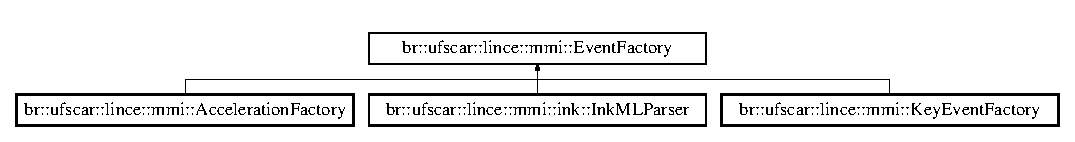
\includegraphics[height=1.45833cm]{classbr_1_1ufscar_1_1lince_1_1mmi_1_1EventFactory}
\end{center}
\end{figure}
\subsection*{Public Member Functions}
\begin{DoxyCompactItemize}
\item 
virtual \hyperlink{classbr_1_1ufscar_1_1lince_1_1mmi_1_1EventFactory_aeee49ee717f13144e6b1458e73c2a0b2}{$\sim$EventFactory} ()
\item 
virtual \hyperlink{classbr_1_1ufscar_1_1lince_1_1mmi_1_1MMIEvent}{MMIEvent} $\ast$ \hyperlink{classbr_1_1ufscar_1_1lince_1_1mmi_1_1EventFactory_a19ad2165726a29a55c921f569764290b}{CreateEvent} (\hyperlink{structbr_1_1ufscar_1_1lince_1_1mmi_1_1XMLData}{XMLData} $\ast$data)=0
\end{DoxyCompactItemize}


\subsection{Constructor \& Destructor Documentation}
\hypertarget{classbr_1_1ufscar_1_1lince_1_1mmi_1_1EventFactory_aeee49ee717f13144e6b1458e73c2a0b2}{
\index{br::ufscar::lince::mmi::EventFactory@{br::ufscar::lince::mmi::EventFactory}!$\sim$EventFactory@{$\sim$EventFactory}}
\index{$\sim$EventFactory@{$\sim$EventFactory}!br::ufscar::lince::mmi::EventFactory@{br::ufscar::lince::mmi::EventFactory}}
\subsubsection[{$\sim$EventFactory}]{\setlength{\rightskip}{0pt plus 5cm}virtual br::ufscar::lince::mmi::EventFactory::$\sim$EventFactory ()\hspace{0.3cm}{\ttfamily  \mbox{[}inline, virtual\mbox{]}}}}
\label{classbr_1_1ufscar_1_1lince_1_1mmi_1_1EventFactory_aeee49ee717f13144e6b1458e73c2a0b2}


\subsection{Member Function Documentation}
\hypertarget{classbr_1_1ufscar_1_1lince_1_1mmi_1_1EventFactory_a19ad2165726a29a55c921f569764290b}{
\index{br::ufscar::lince::mmi::EventFactory@{br::ufscar::lince::mmi::EventFactory}!CreateEvent@{CreateEvent}}
\index{CreateEvent@{CreateEvent}!br::ufscar::lince::mmi::EventFactory@{br::ufscar::lince::mmi::EventFactory}}
\subsubsection[{CreateEvent}]{\setlength{\rightskip}{0pt plus 5cm}virtual {\bf MMIEvent}$\ast$ br::ufscar::lince::mmi::EventFactory::CreateEvent ({\bf XMLData} $\ast$ {\em data})\hspace{0.3cm}{\ttfamily  \mbox{[}pure virtual\mbox{]}}}}
\label{classbr_1_1ufscar_1_1lince_1_1mmi_1_1EventFactory_a19ad2165726a29a55c921f569764290b}


Implemented in \hyperlink{classbr_1_1ufscar_1_1lince_1_1mmi_1_1AccelerationFactory_a5b8858d27f1b956b6c1f27648c010d74}{br::ufscar::lince::mmi::AccelerationFactory}, \hyperlink{classbr_1_1ufscar_1_1lince_1_1mmi_1_1ink_1_1InkMLParser_aeb533c915bd5909319e3195f14993afa}{br::ufscar::lince::mmi::ink::InkMLParser}, and \hyperlink{classbr_1_1ufscar_1_1lince_1_1mmi_1_1KeyEventFactory_a838221bf5491967315a7475691e72103}{br::ufscar::lince::mmi::KeyEventFactory}.



The documentation for this class was generated from the following file:\begin{DoxyCompactItemize}
\item 
include/\hyperlink{EventFactory_8h}{EventFactory.h}\end{DoxyCompactItemize}

\hypertarget{classbr_1_1ufscar_1_1lince_1_1mmi_1_1EventParser}{
\section{br::ufscar::lince::mmi::EventParser Class Reference}
\label{classbr_1_1ufscar_1_1lince_1_1mmi_1_1EventParser}\index{br::ufscar::lince::mmi::EventParser@{br::ufscar::lince::mmi::EventParser}}
}


{\ttfamily \#include $<$EventParser.h$>$}

\subsection*{Public Member Functions}
\begin{DoxyCompactItemize}
\item 
\hyperlink{classbr_1_1ufscar_1_1lince_1_1mmi_1_1MMIEvent}{MMIEvent} $\ast$ \hyperlink{classbr_1_1ufscar_1_1lince_1_1mmi_1_1EventParser_a1af73dd394ee69726f59893cf44fd6cb}{ParseXMLEvent} (\hyperlink{structbr_1_1ufscar_1_1lince_1_1mmi_1_1XMLData}{XMLData} $\ast$data)
\end{DoxyCompactItemize}
\subsection*{Static Public Member Functions}
\begin{DoxyCompactItemize}
\item 
static \hyperlink{classbr_1_1ufscar_1_1lince_1_1mmi_1_1EventParser}{EventParser} $\ast$ \hyperlink{classbr_1_1ufscar_1_1lince_1_1mmi_1_1EventParser_a83a5e79fec5383e011c86a04cc1be477}{getInstance} ()
\end{DoxyCompactItemize}


\subsection{Member Function Documentation}
\hypertarget{classbr_1_1ufscar_1_1lince_1_1mmi_1_1EventParser_a83a5e79fec5383e011c86a04cc1be477}{
\index{br::ufscar::lince::mmi::EventParser@{br::ufscar::lince::mmi::EventParser}!getInstance@{getInstance}}
\index{getInstance@{getInstance}!br::ufscar::lince::mmi::EventParser@{br::ufscar::lince::mmi::EventParser}}
\subsubsection[{getInstance}]{\setlength{\rightskip}{0pt plus 5cm}static {\bf EventParser}$\ast$ br::ufscar::lince::mmi::EventParser::getInstance ()\hspace{0.3cm}{\ttfamily  \mbox{[}static\mbox{]}}}}
\label{classbr_1_1ufscar_1_1lince_1_1mmi_1_1EventParser_a83a5e79fec5383e011c86a04cc1be477}
\hypertarget{classbr_1_1ufscar_1_1lince_1_1mmi_1_1EventParser_a1af73dd394ee69726f59893cf44fd6cb}{
\index{br::ufscar::lince::mmi::EventParser@{br::ufscar::lince::mmi::EventParser}!ParseXMLEvent@{ParseXMLEvent}}
\index{ParseXMLEvent@{ParseXMLEvent}!br::ufscar::lince::mmi::EventParser@{br::ufscar::lince::mmi::EventParser}}
\subsubsection[{ParseXMLEvent}]{\setlength{\rightskip}{0pt plus 5cm}{\bf MMIEvent}$\ast$ br::ufscar::lince::mmi::EventParser::ParseXMLEvent ({\bf XMLData} $\ast$ {\em data})}}
\label{classbr_1_1ufscar_1_1lince_1_1mmi_1_1EventParser_a1af73dd394ee69726f59893cf44fd6cb}


The documentation for this class was generated from the following file:\begin{DoxyCompactItemize}
\item 
include/\hyperlink{EventParser_8h}{EventParser.h}\end{DoxyCompactItemize}

\hypertarget{classbr_1_1ufscar_1_1lince_1_1mmi_1_1ink_1_1GlobalFunction}{
\section{br::ufscar::lince::mmi::ink::GlobalFunction Class Reference}
\label{classbr_1_1ufscar_1_1lince_1_1mmi_1_1ink_1_1GlobalFunction}\index{br::ufscar::lince::mmi::ink::GlobalFunction@{br::ufscar::lince::mmi::ink::GlobalFunction}}
}


Classe que possui métodos úteis para a realização do parser de um InkML.  




{\ttfamily \#include $<$Utility.h$>$}

\subsection*{Static Public Member Functions}
\begin{DoxyCompactItemize}
\item 
static char $\ast$ \hyperlink{classbr_1_1ufscar_1_1lince_1_1mmi_1_1ink_1_1GlobalFunction_a0ef032da8c546e4d12c460efecdffd92}{checkAndRemoveHash} (char $\ast$str)
\item 
static char $\ast$ \hyperlink{classbr_1_1ufscar_1_1lince_1_1mmi_1_1ink_1_1GlobalFunction_a210632b3793a4a8d29cb11eb694548ea}{removeVelocity} (char $\ast$str)
\item 
static char $\ast$ \hyperlink{classbr_1_1ufscar_1_1lince_1_1mmi_1_1ink_1_1GlobalFunction_a05274945e1682ee836877acc4dbab7f8}{decodeError} (\hyperlink{namespacebr_1_1ufscar_1_1lince_1_1mmi_1_1ink_a682c285834346cbf7587dd58c9832fe4}{InkMLError} errorNo)
\item 
static char $\ast$ \hyperlink{classbr_1_1ufscar_1_1lince_1_1mmi_1_1ink_1_1GlobalFunction_ac28d7d2119005e2f55cfa28ec1efce13}{toLower} (char $\ast$s)
\end{DoxyCompactItemize}


\subsection{Detailed Description}
Classe que possui métodos úteis para a realização do parser de um InkML. Mais informações em \href{http://sourceforge.net/apps/trac/inkmltk/wiki/InkMLLib}{\tt http://sourceforge.net/apps/trac/inkmltk/wiki/InkMLLib} 

\subsection{Member Function Documentation}
\hypertarget{classbr_1_1ufscar_1_1lince_1_1mmi_1_1ink_1_1GlobalFunction_a0ef032da8c546e4d12c460efecdffd92}{
\index{br::ufscar::lince::mmi::ink::GlobalFunction@{br::ufscar::lince::mmi::ink::GlobalFunction}!checkAndRemoveHash@{checkAndRemoveHash}}
\index{checkAndRemoveHash@{checkAndRemoveHash}!br::ufscar::lince::mmi::ink::GlobalFunction@{br::ufscar::lince::mmi::ink::GlobalFunction}}
\subsubsection[{checkAndRemoveHash}]{\setlength{\rightskip}{0pt plus 5cm}static char$\ast$ br::ufscar::lince::mmi::ink::GlobalFunction::checkAndRemoveHash (char $\ast$ {\em str})\hspace{0.3cm}{\ttfamily  \mbox{[}static\mbox{]}}}}
\label{classbr_1_1ufscar_1_1lince_1_1mmi_1_1ink_1_1GlobalFunction_a0ef032da8c546e4d12c460efecdffd92}
\hypertarget{classbr_1_1ufscar_1_1lince_1_1mmi_1_1ink_1_1GlobalFunction_a05274945e1682ee836877acc4dbab7f8}{
\index{br::ufscar::lince::mmi::ink::GlobalFunction@{br::ufscar::lince::mmi::ink::GlobalFunction}!decodeError@{decodeError}}
\index{decodeError@{decodeError}!br::ufscar::lince::mmi::ink::GlobalFunction@{br::ufscar::lince::mmi::ink::GlobalFunction}}
\subsubsection[{decodeError}]{\setlength{\rightskip}{0pt plus 5cm}static char$\ast$ br::ufscar::lince::mmi::ink::GlobalFunction::decodeError ({\bf InkMLError} {\em errorNo})\hspace{0.3cm}{\ttfamily  \mbox{[}static\mbox{]}}}}
\label{classbr_1_1ufscar_1_1lince_1_1mmi_1_1ink_1_1GlobalFunction_a05274945e1682ee836877acc4dbab7f8}
\hypertarget{classbr_1_1ufscar_1_1lince_1_1mmi_1_1ink_1_1GlobalFunction_a210632b3793a4a8d29cb11eb694548ea}{
\index{br::ufscar::lince::mmi::ink::GlobalFunction@{br::ufscar::lince::mmi::ink::GlobalFunction}!removeVelocity@{removeVelocity}}
\index{removeVelocity@{removeVelocity}!br::ufscar::lince::mmi::ink::GlobalFunction@{br::ufscar::lince::mmi::ink::GlobalFunction}}
\subsubsection[{removeVelocity}]{\setlength{\rightskip}{0pt plus 5cm}static char$\ast$ br::ufscar::lince::mmi::ink::GlobalFunction::removeVelocity (char $\ast$ {\em str})\hspace{0.3cm}{\ttfamily  \mbox{[}static\mbox{]}}}}
\label{classbr_1_1ufscar_1_1lince_1_1mmi_1_1ink_1_1GlobalFunction_a210632b3793a4a8d29cb11eb694548ea}
\hypertarget{classbr_1_1ufscar_1_1lince_1_1mmi_1_1ink_1_1GlobalFunction_ac28d7d2119005e2f55cfa28ec1efce13}{
\index{br::ufscar::lince::mmi::ink::GlobalFunction@{br::ufscar::lince::mmi::ink::GlobalFunction}!toLower@{toLower}}
\index{toLower@{toLower}!br::ufscar::lince::mmi::ink::GlobalFunction@{br::ufscar::lince::mmi::ink::GlobalFunction}}
\subsubsection[{toLower}]{\setlength{\rightskip}{0pt plus 5cm}static char$\ast$ br::ufscar::lince::mmi::ink::GlobalFunction::toLower (char $\ast$ {\em s})\hspace{0.3cm}{\ttfamily  \mbox{[}static\mbox{]}}}}
\label{classbr_1_1ufscar_1_1lince_1_1mmi_1_1ink_1_1GlobalFunction_ac28d7d2119005e2f55cfa28ec1efce13}


The documentation for this class was generated from the following file:\begin{DoxyCompactItemize}
\item 
include/ink/\hyperlink{Utility_8h}{Utility.h}\end{DoxyCompactItemize}

\hypertarget{classbr_1_1ufscar_1_1lince_1_1mmi_1_1IDeviceComm}{
\section{br::ufscar::lince::mmi::IDeviceComm Class Reference}
\label{classbr_1_1ufscar_1_1lince_1_1mmi_1_1IDeviceComm}\index{br::ufscar::lince::mmi::IDeviceComm@{br::ufscar::lince::mmi::IDeviceComm}}
}


This abstract class represents a device that can generate multimodal events.  




{\ttfamily \#include $<$IDeviceComm.h$>$}

Inheritance diagram for br::ufscar::lince::mmi::IDeviceComm:\begin{figure}[H]
\begin{center}
\leavevmode
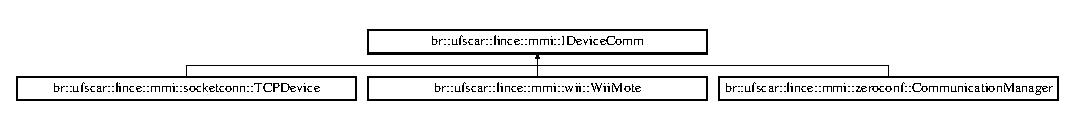
\includegraphics[height=1.1245cm]{classbr_1_1ufscar_1_1lince_1_1mmi_1_1IDeviceComm}
\end{center}
\end{figure}
\subsection*{Public Member Functions}
\begin{DoxyCompactItemize}
\item 
virtual void \hyperlink{classbr_1_1ufscar_1_1lince_1_1mmi_1_1IDeviceComm_a53f48993f294b9a755125b6ccdb06ad4}{connect} ()=0
\begin{DoxyCompactList}\small\item\em This method stabilishes a connect between the device and the \hyperlink{classbr_1_1ufscar_1_1lince_1_1mmi_1_1MMIManager}{MMIManager}, allowing the device reports his multimodal events. \item\end{DoxyCompactList}\item 
virtual void \hyperlink{classbr_1_1ufscar_1_1lince_1_1mmi_1_1IDeviceComm_ad3791cf1ab234f4a6b464c3f614c78c6}{disconnect} ()=0
\begin{DoxyCompactList}\small\item\em This method finishes the connection between the devica and \hyperlink{classbr_1_1ufscar_1_1lince_1_1mmi_1_1MMIManager}{MMIManager}. \item\end{DoxyCompactList}\item 
virtual void \hyperlink{classbr_1_1ufscar_1_1lince_1_1mmi_1_1IDeviceComm_a0249a13030b4df9b50778723421375d9}{sendToDevice} (vector$<$ string $>$ $\ast$args)=0
\begin{DoxyCompactList}\small\item\em This method allows send a message to the device. \item\end{DoxyCompactList}\item 
virtual string \hyperlink{classbr_1_1ufscar_1_1lince_1_1mmi_1_1IDeviceComm_a4ae69c19445713ddc9fda351555c1ac2}{getDeviceId} ()=0
\begin{DoxyCompactList}\small\item\em This method return the id of the device. \item\end{DoxyCompactList}\item 
virtual void \hyperlink{classbr_1_1ufscar_1_1lince_1_1mmi_1_1IDeviceComm_a9c173ebb83a502e78143a52fc7d87a80}{release} ()=0
\begin{DoxyCompactList}\small\item\em This method make the device reset its internals variables. \item\end{DoxyCompactList}\end{DoxyCompactItemize}
\subsection*{Protected Member Functions}
\begin{DoxyCompactItemize}
\item 
virtual \hyperlink{classbr_1_1ufscar_1_1lince_1_1mmi_1_1IDeviceComm_a413107eeac6c3141af8908d601a8de4a}{$\sim$IDeviceComm} ()
\begin{DoxyCompactList}\small\item\em Generic Destructor. \item\end{DoxyCompactList}\end{DoxyCompactItemize}


\subsection{Detailed Description}
This abstract class represents a device that can generate multimodal events. 

\subsection{Constructor \& Destructor Documentation}
\hypertarget{classbr_1_1ufscar_1_1lince_1_1mmi_1_1IDeviceComm_a413107eeac6c3141af8908d601a8de4a}{
\index{br::ufscar::lince::mmi::IDeviceComm@{br::ufscar::lince::mmi::IDeviceComm}!$\sim$IDeviceComm@{$\sim$IDeviceComm}}
\index{$\sim$IDeviceComm@{$\sim$IDeviceComm}!br::ufscar::lince::mmi::IDeviceComm@{br::ufscar::lince::mmi::IDeviceComm}}
\subsubsection[{$\sim$IDeviceComm}]{\setlength{\rightskip}{0pt plus 5cm}virtual br::ufscar::lince::mmi::IDeviceComm::$\sim$IDeviceComm ()\hspace{0.3cm}{\ttfamily  \mbox{[}inline, protected, virtual\mbox{]}}}}
\label{classbr_1_1ufscar_1_1lince_1_1mmi_1_1IDeviceComm_a413107eeac6c3141af8908d601a8de4a}


Generic Destructor. 



\subsection{Member Function Documentation}
\hypertarget{classbr_1_1ufscar_1_1lince_1_1mmi_1_1IDeviceComm_a53f48993f294b9a755125b6ccdb06ad4}{
\index{br::ufscar::lince::mmi::IDeviceComm@{br::ufscar::lince::mmi::IDeviceComm}!connect@{connect}}
\index{connect@{connect}!br::ufscar::lince::mmi::IDeviceComm@{br::ufscar::lince::mmi::IDeviceComm}}
\subsubsection[{connect}]{\setlength{\rightskip}{0pt plus 5cm}virtual void br::ufscar::lince::mmi::IDeviceComm::connect ()\hspace{0.3cm}{\ttfamily  \mbox{[}pure virtual\mbox{]}}}}
\label{classbr_1_1ufscar_1_1lince_1_1mmi_1_1IDeviceComm_a53f48993f294b9a755125b6ccdb06ad4}


This method stabilishes a connect between the device and the \hyperlink{classbr_1_1ufscar_1_1lince_1_1mmi_1_1MMIManager}{MMIManager}, allowing the device reports his multimodal events. 



Implemented in \hyperlink{classbr_1_1ufscar_1_1lince_1_1mmi_1_1socketconn_1_1TCPDevice_a2a474f7f39371460268525b0a840cd4f}{br::ufscar::lince::mmi::socketconn::TCPDevice}, \hyperlink{classbr_1_1ufscar_1_1lince_1_1mmi_1_1wii_1_1WiiMote_a15e0d1b2ac9fde887e870aeb597c0dc8}{br::ufscar::lince::mmi::wii::WiiMote}, and \hyperlink{classbr_1_1ufscar_1_1lince_1_1mmi_1_1zeroconf_1_1CommunicationManager_a580a75f652a1b1e233b6075f740555e1}{br::ufscar::lince::mmi::zeroconf::CommunicationManager}.

\hypertarget{classbr_1_1ufscar_1_1lince_1_1mmi_1_1IDeviceComm_ad3791cf1ab234f4a6b464c3f614c78c6}{
\index{br::ufscar::lince::mmi::IDeviceComm@{br::ufscar::lince::mmi::IDeviceComm}!disconnect@{disconnect}}
\index{disconnect@{disconnect}!br::ufscar::lince::mmi::IDeviceComm@{br::ufscar::lince::mmi::IDeviceComm}}
\subsubsection[{disconnect}]{\setlength{\rightskip}{0pt plus 5cm}virtual void br::ufscar::lince::mmi::IDeviceComm::disconnect ()\hspace{0.3cm}{\ttfamily  \mbox{[}pure virtual\mbox{]}}}}
\label{classbr_1_1ufscar_1_1lince_1_1mmi_1_1IDeviceComm_ad3791cf1ab234f4a6b464c3f614c78c6}


This method finishes the connection between the devica and \hyperlink{classbr_1_1ufscar_1_1lince_1_1mmi_1_1MMIManager}{MMIManager}. 



Implemented in \hyperlink{classbr_1_1ufscar_1_1lince_1_1mmi_1_1socketconn_1_1TCPDevice_a5b1eca485752195ce49f03475229ca1f}{br::ufscar::lince::mmi::socketconn::TCPDevice}, \hyperlink{classbr_1_1ufscar_1_1lince_1_1mmi_1_1wii_1_1WiiMote_a44aa8cf98660392a91045e4892a9e65a}{br::ufscar::lince::mmi::wii::WiiMote}, and \hyperlink{classbr_1_1ufscar_1_1lince_1_1mmi_1_1zeroconf_1_1CommunicationManager_a1c41c5541bf5c02b78f3dc10a045c7f6}{br::ufscar::lince::mmi::zeroconf::CommunicationManager}.

\hypertarget{classbr_1_1ufscar_1_1lince_1_1mmi_1_1IDeviceComm_a4ae69c19445713ddc9fda351555c1ac2}{
\index{br::ufscar::lince::mmi::IDeviceComm@{br::ufscar::lince::mmi::IDeviceComm}!getDeviceId@{getDeviceId}}
\index{getDeviceId@{getDeviceId}!br::ufscar::lince::mmi::IDeviceComm@{br::ufscar::lince::mmi::IDeviceComm}}
\subsubsection[{getDeviceId}]{\setlength{\rightskip}{0pt plus 5cm}virtual string br::ufscar::lince::mmi::IDeviceComm::getDeviceId ()\hspace{0.3cm}{\ttfamily  \mbox{[}pure virtual\mbox{]}}}}
\label{classbr_1_1ufscar_1_1lince_1_1mmi_1_1IDeviceComm_a4ae69c19445713ddc9fda351555c1ac2}


This method return the id of the device. 

\begin{DoxyReturn}{Returns}
Device identification. 
\end{DoxyReturn}


Implemented in \hyperlink{classbr_1_1ufscar_1_1lince_1_1mmi_1_1socketconn_1_1TCPDevice_aa45bb0937e02c3d58c9923c369408e5a}{br::ufscar::lince::mmi::socketconn::TCPDevice}, \hyperlink{classbr_1_1ufscar_1_1lince_1_1mmi_1_1wii_1_1WiiMote_a125dc3805711f4b5fa9327ebf719e035}{br::ufscar::lince::mmi::wii::WiiMote}, and \hyperlink{classbr_1_1ufscar_1_1lince_1_1mmi_1_1zeroconf_1_1CommunicationManager_ac81ba73dafe9e2ca558fad5d46f09e8c}{br::ufscar::lince::mmi::zeroconf::CommunicationManager}.

\hypertarget{classbr_1_1ufscar_1_1lince_1_1mmi_1_1IDeviceComm_a9c173ebb83a502e78143a52fc7d87a80}{
\index{br::ufscar::lince::mmi::IDeviceComm@{br::ufscar::lince::mmi::IDeviceComm}!release@{release}}
\index{release@{release}!br::ufscar::lince::mmi::IDeviceComm@{br::ufscar::lince::mmi::IDeviceComm}}
\subsubsection[{release}]{\setlength{\rightskip}{0pt plus 5cm}virtual void br::ufscar::lince::mmi::IDeviceComm::release ()\hspace{0.3cm}{\ttfamily  \mbox{[}pure virtual\mbox{]}}}}
\label{classbr_1_1ufscar_1_1lince_1_1mmi_1_1IDeviceComm_a9c173ebb83a502e78143a52fc7d87a80}


This method make the device reset its internals variables. 



Implemented in \hyperlink{classbr_1_1ufscar_1_1lince_1_1mmi_1_1socketconn_1_1TCPDevice_a4004f2bdb8466c2613654469d0863f78}{br::ufscar::lince::mmi::socketconn::TCPDevice}, \hyperlink{classbr_1_1ufscar_1_1lince_1_1mmi_1_1wii_1_1WiiMote_a4d17da2514583aa3787a1d9fda1cd74c}{br::ufscar::lince::mmi::wii::WiiMote}, and \hyperlink{classbr_1_1ufscar_1_1lince_1_1mmi_1_1zeroconf_1_1CommunicationManager_aef7bfab9cd63ab8e75fb0782e019574b}{br::ufscar::lince::mmi::zeroconf::CommunicationManager}.

\hypertarget{classbr_1_1ufscar_1_1lince_1_1mmi_1_1IDeviceComm_a0249a13030b4df9b50778723421375d9}{
\index{br::ufscar::lince::mmi::IDeviceComm@{br::ufscar::lince::mmi::IDeviceComm}!sendToDevice@{sendToDevice}}
\index{sendToDevice@{sendToDevice}!br::ufscar::lince::mmi::IDeviceComm@{br::ufscar::lince::mmi::IDeviceComm}}
\subsubsection[{sendToDevice}]{\setlength{\rightskip}{0pt plus 5cm}virtual void br::ufscar::lince::mmi::IDeviceComm::sendToDevice (vector$<$ string $>$ $\ast$ {\em args})\hspace{0.3cm}{\ttfamily  \mbox{[}pure virtual\mbox{]}}}}
\label{classbr_1_1ufscar_1_1lince_1_1mmi_1_1IDeviceComm_a0249a13030b4df9b50778723421375d9}


This method allows send a message to the device. 


\begin{DoxyParams}{Parameters}
\item[{\em args}]A array of strings that will contain the message. \end{DoxyParams}


Implemented in \hyperlink{classbr_1_1ufscar_1_1lince_1_1mmi_1_1socketconn_1_1TCPDevice_a533e8c0d49d2418a244e46242dc70d99}{br::ufscar::lince::mmi::socketconn::TCPDevice}, \hyperlink{classbr_1_1ufscar_1_1lince_1_1mmi_1_1wii_1_1WiiMote_acd1fe851dd5909ee3cbd0fa23a070f0e}{br::ufscar::lince::mmi::wii::WiiMote}, and \hyperlink{classbr_1_1ufscar_1_1lince_1_1mmi_1_1zeroconf_1_1CommunicationManager_a40b30969966a6517d21cf9a1cf5c3da8}{br::ufscar::lince::mmi::zeroconf::CommunicationManager}.



The documentation for this class was generated from the following file:\begin{DoxyCompactItemize}
\item 
include/\hyperlink{IDeviceComm_8h}{IDeviceComm.h}\end{DoxyCompactItemize}

\hypertarget{classbr_1_1ufscar_1_1lince_1_1mmi_1_1ink_1_1Ink}{
\section{br::ufscar::lince::mmi::ink::Ink Class Reference}
\label{classbr_1_1ufscar_1_1lince_1_1mmi_1_1ink_1_1Ink}\index{br::ufscar::lince::mmi::ink::Ink@{br::ufscar::lince::mmi::ink::Ink}}
}


Classe que representa dados de tinta contidos em um MultimodalInputEvent.  




{\ttfamily \#include $<$Ink.h$>$}

Inheritance diagram for br::ufscar::lince::mmi::ink::Ink:\begin{figure}[H]
\begin{center}
\leavevmode
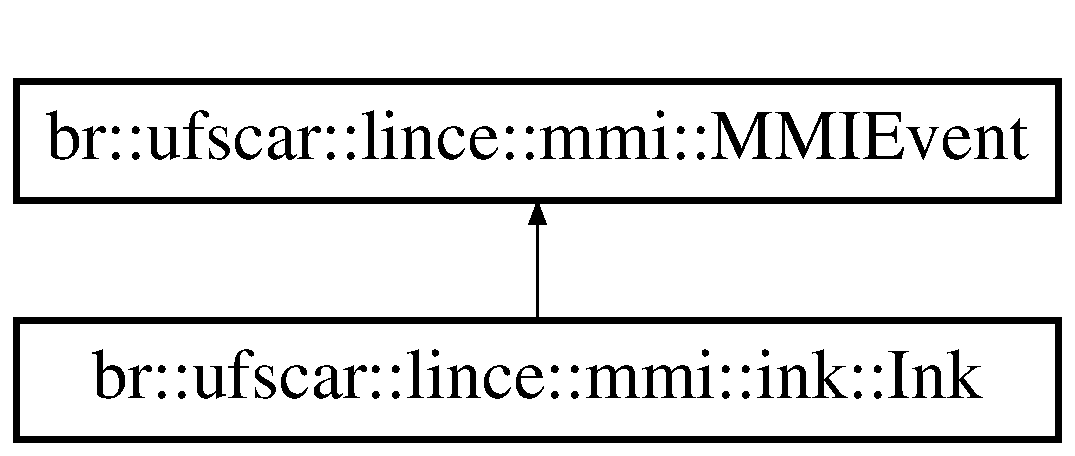
\includegraphics[height=2cm]{classbr_1_1ufscar_1_1lince_1_1mmi_1_1ink_1_1Ink}
\end{center}
\end{figure}
\subsection*{Public Member Functions}
\begin{DoxyCompactItemize}
\item 
\hyperlink{classbr_1_1ufscar_1_1lince_1_1mmi_1_1ink_1_1Ink_ada758b5f8c862e96b3bc0ab8ab5c305e}{Ink} ()
\begin{DoxyCompactList}\small\item\em Desc -\/ constructor to create an ink document. \item\end{DoxyCompactList}\item 
void \hyperlink{classbr_1_1ufscar_1_1lince_1_1mmi_1_1ink_1_1Ink_a020076b1bfae4c76a9fa42f87aa618a7}{addDefinitions} (Definitions $\ast$definitions)
\begin{DoxyCompactList}\small\item\em Desc -\/ assign the definitions state of this ink document. \item\end{DoxyCompactList}\item 
Definitions $\ast$ \hyperlink{classbr_1_1ufscar_1_1lince_1_1mmi_1_1ink_1_1Ink_a1a6e44946dd40a11af964dabc129d11c}{getDefinitions} ()
\begin{DoxyCompactList}\small\item\em Desc -\/ function to get the definitions state of this ink document. \item\end{DoxyCompactList}\item 
void \hyperlink{classbr_1_1ufscar_1_1lince_1_1mmi_1_1ink_1_1Ink_a9fdefbe3184e360412b74675b853ad16}{addTrace} (\hyperlink{classbr_1_1ufscar_1_1lince_1_1mmi_1_1ink_1_1Trace}{Trace} trace)
\begin{DoxyCompactList}\small\item\em Desc -\/ function to add a \hyperlink{classbr_1_1ufscar_1_1lince_1_1mmi_1_1ink_1_1Trace}{Trace} to this ink document. \item\end{DoxyCompactList}\item 
void \hyperlink{classbr_1_1ufscar_1_1lince_1_1mmi_1_1ink_1_1Ink_a6f102e2395f0ebac1d4044291389cbf2}{normalizeTracePoint} (long width, long height)
\begin{DoxyCompactList}\small\item\em Desc -\/ function to normalize trace sample point data to fit within the given boundary box for rendering. \item\end{DoxyCompactList}\end{DoxyCompactItemize}
\subsection*{Data Fields}
\begin{DoxyCompactItemize}
\item 
\hyperlink{structbr_1_1ufscar_1_1lince_1_1mmi_1_1ink_1_1structBoundingBox}{BoundingBox} $\ast$ \hyperlink{classbr_1_1ufscar_1_1lince_1_1mmi_1_1ink_1_1Ink_aba7f2aa5e6398319ff07182898bc21a8}{boundingBox}
\begin{DoxyCompactList}\small\item\em Desc -\/ To capture the boundary of the rectangle inside whice the traces of this ink document would be rendered. \item\end{DoxyCompactList}\item 
vector$<$ \hyperlink{classbr_1_1ufscar_1_1lince_1_1mmi_1_1ink_1_1Trace}{Trace} $>$ $\ast$ \hyperlink{classbr_1_1ufscar_1_1lince_1_1mmi_1_1ink_1_1Ink_a9dee6cfd152a6de770ac10b40e761ef8}{vectTrace}
\begin{DoxyCompactList}\small\item\em Desc -\/ To hold all traces of this ink document. \item\end{DoxyCompactList}\item 
Context $\ast$ \hyperlink{classbr_1_1ufscar_1_1lince_1_1mmi_1_1ink_1_1Ink_a13e685700da2ba95fa84c48b7aa339f9}{currentContext}
\begin{DoxyCompactList}\small\item\em Desc -\/ handle to the current context of this ink document. \item\end{DoxyCompactList}\end{DoxyCompactItemize}


\subsection{Detailed Description}
Classe que representa dados de tinta contidos em um MultimodalInputEvent. Mais informações em \href{http://sourceforge.net/apps/trac/inkmltk/wiki/InkMLLib}{\tt http://sourceforge.net/apps/trac/inkmltk/wiki/InkMLLib} 

\subsection{Constructor \& Destructor Documentation}
\hypertarget{classbr_1_1ufscar_1_1lince_1_1mmi_1_1ink_1_1Ink_ada758b5f8c862e96b3bc0ab8ab5c305e}{
\index{br::ufscar::lince::mmi::ink::Ink@{br::ufscar::lince::mmi::ink::Ink}!Ink@{Ink}}
\index{Ink@{Ink}!br::ufscar::lince::mmi::ink::Ink@{br::ufscar::lince::mmi::ink::Ink}}
\subsubsection[{Ink}]{\setlength{\rightskip}{0pt plus 5cm}br::ufscar::lince::mmi::ink::Ink::Ink ()}}
\label{classbr_1_1ufscar_1_1lince_1_1mmi_1_1ink_1_1Ink_ada758b5f8c862e96b3bc0ab8ab5c305e}


Desc -\/ constructor to create an ink document. 



\subsection{Member Function Documentation}
\hypertarget{classbr_1_1ufscar_1_1lince_1_1mmi_1_1ink_1_1Ink_a020076b1bfae4c76a9fa42f87aa618a7}{
\index{br::ufscar::lince::mmi::ink::Ink@{br::ufscar::lince::mmi::ink::Ink}!addDefinitions@{addDefinitions}}
\index{addDefinitions@{addDefinitions}!br::ufscar::lince::mmi::ink::Ink@{br::ufscar::lince::mmi::ink::Ink}}
\subsubsection[{addDefinitions}]{\setlength{\rightskip}{0pt plus 5cm}void br::ufscar::lince::mmi::ink::Ink::addDefinitions (Definitions $\ast$ {\em definitions})\hspace{0.3cm}{\ttfamily  \mbox{[}inline\mbox{]}}}}
\label{classbr_1_1ufscar_1_1lince_1_1mmi_1_1ink_1_1Ink_a020076b1bfae4c76a9fa42f87aa618a7}


Desc -\/ assign the definitions state of this ink document. 

\hypertarget{classbr_1_1ufscar_1_1lince_1_1mmi_1_1ink_1_1Ink_a9fdefbe3184e360412b74675b853ad16}{
\index{br::ufscar::lince::mmi::ink::Ink@{br::ufscar::lince::mmi::ink::Ink}!addTrace@{addTrace}}
\index{addTrace@{addTrace}!br::ufscar::lince::mmi::ink::Ink@{br::ufscar::lince::mmi::ink::Ink}}
\subsubsection[{addTrace}]{\setlength{\rightskip}{0pt plus 5cm}void br::ufscar::lince::mmi::ink::Ink::addTrace ({\bf Trace} {\em trace})\hspace{0.3cm}{\ttfamily  \mbox{[}inline\mbox{]}}}}
\label{classbr_1_1ufscar_1_1lince_1_1mmi_1_1ink_1_1Ink_a9fdefbe3184e360412b74675b853ad16}


Desc -\/ function to add a \hyperlink{classbr_1_1ufscar_1_1lince_1_1mmi_1_1ink_1_1Trace}{Trace} to this ink document. 

\hypertarget{classbr_1_1ufscar_1_1lince_1_1mmi_1_1ink_1_1Ink_a1a6e44946dd40a11af964dabc129d11c}{
\index{br::ufscar::lince::mmi::ink::Ink@{br::ufscar::lince::mmi::ink::Ink}!getDefinitions@{getDefinitions}}
\index{getDefinitions@{getDefinitions}!br::ufscar::lince::mmi::ink::Ink@{br::ufscar::lince::mmi::ink::Ink}}
\subsubsection[{getDefinitions}]{\setlength{\rightskip}{0pt plus 5cm}Definitions$\ast$ br::ufscar::lince::mmi::ink::Ink::getDefinitions ()\hspace{0.3cm}{\ttfamily  \mbox{[}inline\mbox{]}}}}
\label{classbr_1_1ufscar_1_1lince_1_1mmi_1_1ink_1_1Ink_a1a6e44946dd40a11af964dabc129d11c}


Desc -\/ function to get the definitions state of this ink document. 

\hypertarget{classbr_1_1ufscar_1_1lince_1_1mmi_1_1ink_1_1Ink_a6f102e2395f0ebac1d4044291389cbf2}{
\index{br::ufscar::lince::mmi::ink::Ink@{br::ufscar::lince::mmi::ink::Ink}!normalizeTracePoint@{normalizeTracePoint}}
\index{normalizeTracePoint@{normalizeTracePoint}!br::ufscar::lince::mmi::ink::Ink@{br::ufscar::lince::mmi::ink::Ink}}
\subsubsection[{normalizeTracePoint}]{\setlength{\rightskip}{0pt plus 5cm}void br::ufscar::lince::mmi::ink::Ink::normalizeTracePoint (long {\em width}, \/  long {\em height})}}
\label{classbr_1_1ufscar_1_1lince_1_1mmi_1_1ink_1_1Ink_a6f102e2395f0ebac1d4044291389cbf2}


Desc -\/ function to normalize trace sample point data to fit within the given boundary box for rendering. 



\subsection{Field Documentation}
\hypertarget{classbr_1_1ufscar_1_1lince_1_1mmi_1_1ink_1_1Ink_aba7f2aa5e6398319ff07182898bc21a8}{
\index{br::ufscar::lince::mmi::ink::Ink@{br::ufscar::lince::mmi::ink::Ink}!boundingBox@{boundingBox}}
\index{boundingBox@{boundingBox}!br::ufscar::lince::mmi::ink::Ink@{br::ufscar::lince::mmi::ink::Ink}}
\subsubsection[{boundingBox}]{\setlength{\rightskip}{0pt plus 5cm}{\bf BoundingBox}$\ast$ {\bf br::ufscar::lince::mmi::ink::Ink::boundingBox}}}
\label{classbr_1_1ufscar_1_1lince_1_1mmi_1_1ink_1_1Ink_aba7f2aa5e6398319ff07182898bc21a8}


Desc -\/ To capture the boundary of the rectangle inside whice the traces of this ink document would be rendered. 

\hypertarget{classbr_1_1ufscar_1_1lince_1_1mmi_1_1ink_1_1Ink_a13e685700da2ba95fa84c48b7aa339f9}{
\index{br::ufscar::lince::mmi::ink::Ink@{br::ufscar::lince::mmi::ink::Ink}!currentContext@{currentContext}}
\index{currentContext@{currentContext}!br::ufscar::lince::mmi::ink::Ink@{br::ufscar::lince::mmi::ink::Ink}}
\subsubsection[{currentContext}]{\setlength{\rightskip}{0pt plus 5cm}Context$\ast$ {\bf br::ufscar::lince::mmi::ink::Ink::currentContext}}}
\label{classbr_1_1ufscar_1_1lince_1_1mmi_1_1ink_1_1Ink_a13e685700da2ba95fa84c48b7aa339f9}


Desc -\/ handle to the current context of this ink document. 

\hypertarget{classbr_1_1ufscar_1_1lince_1_1mmi_1_1ink_1_1Ink_a9dee6cfd152a6de770ac10b40e761ef8}{
\index{br::ufscar::lince::mmi::ink::Ink@{br::ufscar::lince::mmi::ink::Ink}!vectTrace@{vectTrace}}
\index{vectTrace@{vectTrace}!br::ufscar::lince::mmi::ink::Ink@{br::ufscar::lince::mmi::ink::Ink}}
\subsubsection[{vectTrace}]{\setlength{\rightskip}{0pt plus 5cm}vector$<${\bf Trace}$>$$\ast$ {\bf br::ufscar::lince::mmi::ink::Ink::vectTrace}}}
\label{classbr_1_1ufscar_1_1lince_1_1mmi_1_1ink_1_1Ink_a9dee6cfd152a6de770ac10b40e761ef8}


Desc -\/ To hold all traces of this ink document. 



The documentation for this class was generated from the following file:\begin{DoxyCompactItemize}
\item 
include/ink/\hyperlink{Ink_8h}{Ink.h}\end{DoxyCompactItemize}

\hypertarget{classbr_1_1ufscar_1_1lince_1_1mmi_1_1ink_1_1InkMLParser}{
\section{br::ufscar::lince::mmi::ink::InkMLParser Class Reference}
\label{classbr_1_1ufscar_1_1lince_1_1mmi_1_1ink_1_1InkMLParser}\index{br::ufscar::lince::mmi::ink::InkMLParser@{br::ufscar::lince::mmi::ink::InkMLParser}}
}


Classe responsável por realizar o parser de um InkML, utilizando a biblioteca xerces.  




{\ttfamily \#include $<$InkMLParser.h$>$}

Inheritance diagram for br::ufscar::lince::mmi::ink::InkMLParser:\begin{figure}[H]
\begin{center}
\leavevmode
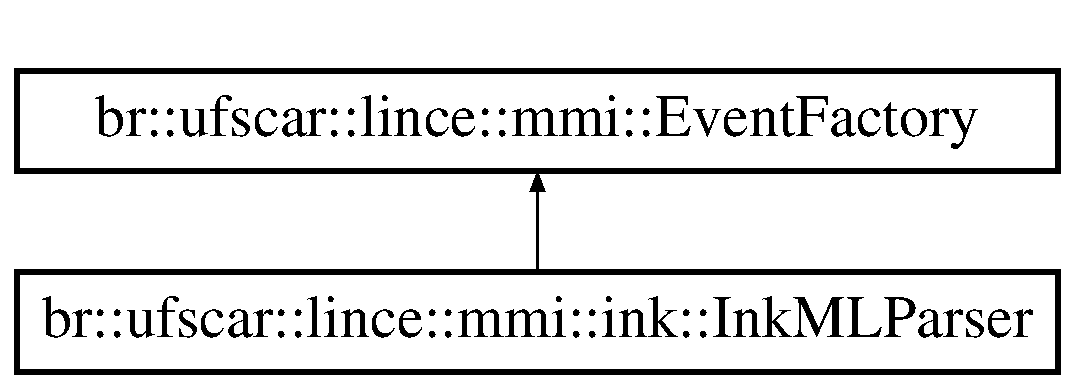
\includegraphics[height=2cm]{classbr_1_1ufscar_1_1lince_1_1mmi_1_1ink_1_1InkMLParser}
\end{center}
\end{figure}
\subsection*{Public Member Functions}
\begin{DoxyCompactItemize}
\item 
\hyperlink{classbr_1_1ufscar_1_1lince_1_1mmi_1_1ink_1_1InkMLParser_a53b502493d849cc8244d5a831c0afe13}{InkMLParser} ()
\begin{DoxyCompactList}\small\item\em Construtor da classe InKMLParser. \item\end{DoxyCompactList}\item 
virtual \hyperlink{classbr_1_1ufscar_1_1lince_1_1mmi_1_1MMIEvent}{MMIEvent} $\ast$ \hyperlink{classbr_1_1ufscar_1_1lince_1_1mmi_1_1ink_1_1InkMLParser_aeb533c915bd5909319e3195f14993afa}{CreateEvent} (\hyperlink{structbr_1_1ufscar_1_1lince_1_1mmi_1_1XMLData}{XMLData} $\ast$data)
\end{DoxyCompactItemize}
\subsection*{Protected Member Functions}
\begin{DoxyCompactItemize}
\item 
void \hyperlink{classbr_1_1ufscar_1_1lince_1_1mmi_1_1ink_1_1InkMLParser_afa63df2f41822c11e28762f3c17b1b43}{parseDefinitions} (DOMElement $\ast$e, \hyperlink{classbr_1_1ufscar_1_1lince_1_1mmi_1_1ink_1_1Ink}{Ink} $\ast$objInk)
\begin{DoxyCompactList}\small\item\em Faz o parser de uma tag \char`\"{}definitions\char`\"{} e acrescenta os dados no objeto da Classe \hyperlink{classbr_1_1ufscar_1_1lince_1_1mmi_1_1ink_1_1Ink}{Ink} recebido. \item\end{DoxyCompactList}\item 
\hyperlink{classbr_1_1ufscar_1_1lince_1_1mmi_1_1ink_1_1Ink}{Ink} $\ast$ \hyperlink{classbr_1_1ufscar_1_1lince_1_1mmi_1_1ink_1_1InkMLParser_a77a83c6281e610f692254e0e2e96f956}{parse} (DOMElement $\ast$inkMLData, \hyperlink{namespacebr_1_1ufscar_1_1lince_1_1mmi_1_1ink_a682c285834346cbf7587dd58c9832fe4}{InkMLError} $\ast$retCode)
\begin{DoxyCompactList}\small\item\em Faz o parser de uma tag \char`\"{}ink\char`\"{} e retorna um objeto da Classe \hyperlink{classbr_1_1ufscar_1_1lince_1_1mmi_1_1ink_1_1Ink}{Ink}. \item\end{DoxyCompactList}\item 
void \hyperlink{classbr_1_1ufscar_1_1lince_1_1mmi_1_1ink_1_1InkMLParser_ab2fdfc15cb9334ff037f2e49dd41fe42}{insertTrace} (DOMElement $\ast$child, \hyperlink{classbr_1_1ufscar_1_1lince_1_1mmi_1_1ink_1_1Ink}{Ink} $\ast$objInk)
\begin{DoxyCompactList}\small\item\em Faz o parser de uma tag \char`\"{}trace\char`\"{} e acrescenta os dados no objeto da Classe \hyperlink{classbr_1_1ufscar_1_1lince_1_1mmi_1_1ink_1_1Ink}{Ink} recebido. \item\end{DoxyCompactList}\end{DoxyCompactItemize}
\subsection*{Protected Attributes}
\begin{DoxyCompactItemize}
\item 
HLoggerPtr \hyperlink{classbr_1_1ufscar_1_1lince_1_1mmi_1_1ink_1_1InkMLParser_aab8a422c5f6b431865f0b848b96f5e35}{logger}
\begin{DoxyCompactList}\small\item\em Responsável pelo controle das mensagens de log. \item\end{DoxyCompactList}\end{DoxyCompactItemize}


\subsection{Detailed Description}
Classe responsável por realizar o parser de um InkML, utilizando a biblioteca xerces. Mais informações em \href{http://sourceforge.net/apps/trac/inkmltk/wiki/InkMLLib}{\tt http://sourceforge.net/apps/trac/inkmltk/wiki/InkMLLib} 

\subsection{Constructor \& Destructor Documentation}
\hypertarget{classbr_1_1ufscar_1_1lince_1_1mmi_1_1ink_1_1InkMLParser_a53b502493d849cc8244d5a831c0afe13}{
\index{br::ufscar::lince::mmi::ink::InkMLParser@{br::ufscar::lince::mmi::ink::InkMLParser}!InkMLParser@{InkMLParser}}
\index{InkMLParser@{InkMLParser}!br::ufscar::lince::mmi::ink::InkMLParser@{br::ufscar::lince::mmi::ink::InkMLParser}}
\subsubsection[{InkMLParser}]{\setlength{\rightskip}{0pt plus 5cm}br::ufscar::lince::mmi::ink::InkMLParser::InkMLParser ()}}
\label{classbr_1_1ufscar_1_1lince_1_1mmi_1_1ink_1_1InkMLParser_a53b502493d849cc8244d5a831c0afe13}


Construtor da classe InKMLParser. 



\subsection{Member Function Documentation}
\hypertarget{classbr_1_1ufscar_1_1lince_1_1mmi_1_1ink_1_1InkMLParser_aeb533c915bd5909319e3195f14993afa}{
\index{br::ufscar::lince::mmi::ink::InkMLParser@{br::ufscar::lince::mmi::ink::InkMLParser}!CreateEvent@{CreateEvent}}
\index{CreateEvent@{CreateEvent}!br::ufscar::lince::mmi::ink::InkMLParser@{br::ufscar::lince::mmi::ink::InkMLParser}}
\subsubsection[{CreateEvent}]{\setlength{\rightskip}{0pt plus 5cm}virtual {\bf MMIEvent}$\ast$ br::ufscar::lince::mmi::ink::InkMLParser::CreateEvent ({\bf XMLData} $\ast$ {\em data})\hspace{0.3cm}{\ttfamily  \mbox{[}virtual\mbox{]}}}}
\label{classbr_1_1ufscar_1_1lince_1_1mmi_1_1ink_1_1InkMLParser_aeb533c915bd5909319e3195f14993afa}


Implements \hyperlink{classbr_1_1ufscar_1_1lince_1_1mmi_1_1EventFactory_a19ad2165726a29a55c921f569764290b}{br::ufscar::lince::mmi::EventFactory}.

\hypertarget{classbr_1_1ufscar_1_1lince_1_1mmi_1_1ink_1_1InkMLParser_ab2fdfc15cb9334ff037f2e49dd41fe42}{
\index{br::ufscar::lince::mmi::ink::InkMLParser@{br::ufscar::lince::mmi::ink::InkMLParser}!insertTrace@{insertTrace}}
\index{insertTrace@{insertTrace}!br::ufscar::lince::mmi::ink::InkMLParser@{br::ufscar::lince::mmi::ink::InkMLParser}}
\subsubsection[{insertTrace}]{\setlength{\rightskip}{0pt plus 5cm}void br::ufscar::lince::mmi::ink::InkMLParser::insertTrace (DOMElement $\ast$ {\em child}, \/  {\bf Ink} $\ast$ {\em objInk})\hspace{0.3cm}{\ttfamily  \mbox{[}protected\mbox{]}}}}
\label{classbr_1_1ufscar_1_1lince_1_1mmi_1_1ink_1_1InkMLParser_ab2fdfc15cb9334ff037f2e49dd41fe42}


Faz o parser de uma tag \char`\"{}trace\char`\"{} e acrescenta os dados no objeto da Classe \hyperlink{classbr_1_1ufscar_1_1lince_1_1mmi_1_1ink_1_1Ink}{Ink} recebido. 


\begin{DoxyParams}{Parameters}
\item[{\em child}]DOMElement a ser parseado \item[{\em objInk}]Instância de \hyperlink{classbr_1_1ufscar_1_1lince_1_1mmi_1_1ink_1_1Ink}{Ink} que receberá os dados parseados \end{DoxyParams}
\hypertarget{classbr_1_1ufscar_1_1lince_1_1mmi_1_1ink_1_1InkMLParser_a77a83c6281e610f692254e0e2e96f956}{
\index{br::ufscar::lince::mmi::ink::InkMLParser@{br::ufscar::lince::mmi::ink::InkMLParser}!parse@{parse}}
\index{parse@{parse}!br::ufscar::lince::mmi::ink::InkMLParser@{br::ufscar::lince::mmi::ink::InkMLParser}}
\subsubsection[{parse}]{\setlength{\rightskip}{0pt plus 5cm}{\bf Ink}$\ast$ br::ufscar::lince::mmi::ink::InkMLParser::parse (DOMElement $\ast$ {\em inkMLData}, \/  {\bf InkMLError} $\ast$ {\em retCode})\hspace{0.3cm}{\ttfamily  \mbox{[}protected\mbox{]}}}}
\label{classbr_1_1ufscar_1_1lince_1_1mmi_1_1ink_1_1InkMLParser_a77a83c6281e610f692254e0e2e96f956}


Faz o parser de uma tag \char`\"{}ink\char`\"{} e retorna um objeto da Classe \hyperlink{classbr_1_1ufscar_1_1lince_1_1mmi_1_1ink_1_1Ink}{Ink}. 


\begin{DoxyParams}{Parameters}
\item[{\em inkMLData}]DOMElement a ser parseado \item[{\em retCode}]Código de erro, caso ocorra, ou NoError em caso de sucesso \end{DoxyParams}
\hypertarget{classbr_1_1ufscar_1_1lince_1_1mmi_1_1ink_1_1InkMLParser_afa63df2f41822c11e28762f3c17b1b43}{
\index{br::ufscar::lince::mmi::ink::InkMLParser@{br::ufscar::lince::mmi::ink::InkMLParser}!parseDefinitions@{parseDefinitions}}
\index{parseDefinitions@{parseDefinitions}!br::ufscar::lince::mmi::ink::InkMLParser@{br::ufscar::lince::mmi::ink::InkMLParser}}
\subsubsection[{parseDefinitions}]{\setlength{\rightskip}{0pt plus 5cm}void br::ufscar::lince::mmi::ink::InkMLParser::parseDefinitions (DOMElement $\ast$ {\em e}, \/  {\bf Ink} $\ast$ {\em objInk})\hspace{0.3cm}{\ttfamily  \mbox{[}protected\mbox{]}}}}
\label{classbr_1_1ufscar_1_1lince_1_1mmi_1_1ink_1_1InkMLParser_afa63df2f41822c11e28762f3c17b1b43}


Faz o parser de uma tag \char`\"{}definitions\char`\"{} e acrescenta os dados no objeto da Classe \hyperlink{classbr_1_1ufscar_1_1lince_1_1mmi_1_1ink_1_1Ink}{Ink} recebido. 


\begin{DoxyParams}{Parameters}
\item[{\em e}]DOMElement a ser parseado \item[{\em objInk}]Instância de \hyperlink{classbr_1_1ufscar_1_1lince_1_1mmi_1_1ink_1_1Ink}{Ink} que receberá os dados parseados \end{DoxyParams}


\subsection{Field Documentation}
\hypertarget{classbr_1_1ufscar_1_1lince_1_1mmi_1_1ink_1_1InkMLParser_aab8a422c5f6b431865f0b848b96f5e35}{
\index{br::ufscar::lince::mmi::ink::InkMLParser@{br::ufscar::lince::mmi::ink::InkMLParser}!logger@{logger}}
\index{logger@{logger}!br::ufscar::lince::mmi::ink::InkMLParser@{br::ufscar::lince::mmi::ink::InkMLParser}}
\subsubsection[{logger}]{\setlength{\rightskip}{0pt plus 5cm}HLoggerPtr {\bf br::ufscar::lince::mmi::ink::InkMLParser::logger}\hspace{0.3cm}{\ttfamily  \mbox{[}protected\mbox{]}}}}
\label{classbr_1_1ufscar_1_1lince_1_1mmi_1_1ink_1_1InkMLParser_aab8a422c5f6b431865f0b848b96f5e35}


Responsável pelo controle das mensagens de log. 



The documentation for this class was generated from the following file:\begin{DoxyCompactItemize}
\item 
include/ink/\hyperlink{InkMLParser_8h}{InkMLParser.h}\end{DoxyCompactItemize}

\hypertarget{classbr_1_1ufscar_1_1lince_1_1mmi_1_1ink_1_1InkSource}{
\section{br::ufscar::lince::mmi::ink::InkSource Class Reference}
\label{classbr_1_1ufscar_1_1lince_1_1mmi_1_1ink_1_1InkSource}\index{br::ufscar::lince::mmi::ink::InkSource@{br::ufscar::lince::mmi::ink::InkSource}}
}


Clase que representa a \hyperlink{classbr_1_1ufscar_1_1lince_1_1mmi_1_1ink_1_1InkSource}{InkSource} de um InkML.  




{\ttfamily \#include $<$InkSource.h$>$}

\subsection*{Public Member Functions}
\begin{DoxyCompactItemize}
\item 
\hyperlink{classbr_1_1ufscar_1_1lince_1_1mmi_1_1ink_1_1InkSource_a5888d2b6cd9e1dde2aafa26c006e7f2a}{InkSource} ()
\begin{DoxyCompactList}\small\item\em Construtor. \item\end{DoxyCompactList}\item 
void \hyperlink{classbr_1_1ufscar_1_1lince_1_1mmi_1_1ink_1_1InkSource_a304b6c7e9ef21b86db8a5eb54d3728cc}{addTraceFormat} (\hyperlink{classbr_1_1ufscar_1_1lince_1_1mmi_1_1ink_1_1TraceFormat}{TraceFormat} $\ast$traceFormat)
\begin{DoxyCompactList}\small\item\em Adiciona um traceFormat. \item\end{DoxyCompactList}\end{DoxyCompactItemize}


\subsection{Detailed Description}
Clase que representa a \hyperlink{classbr_1_1ufscar_1_1lince_1_1mmi_1_1ink_1_1InkSource}{InkSource} de um InkML. Mais informações em \href{http://sourceforge.net/apps/trac/inkmltk/wiki/InkMLLib}{\tt http://sourceforge.net/apps/trac/inkmltk/wiki/InkMLLib} 

\subsection{Constructor \& Destructor Documentation}
\hypertarget{classbr_1_1ufscar_1_1lince_1_1mmi_1_1ink_1_1InkSource_a5888d2b6cd9e1dde2aafa26c006e7f2a}{
\index{br::ufscar::lince::mmi::ink::InkSource@{br::ufscar::lince::mmi::ink::InkSource}!InkSource@{InkSource}}
\index{InkSource@{InkSource}!br::ufscar::lince::mmi::ink::InkSource@{br::ufscar::lince::mmi::ink::InkSource}}
\subsubsection[{InkSource}]{\setlength{\rightskip}{0pt plus 5cm}br::ufscar::lince::mmi::ink::InkSource::InkSource ()\hspace{0.3cm}{\ttfamily  \mbox{[}inline\mbox{]}}}}
\label{classbr_1_1ufscar_1_1lince_1_1mmi_1_1ink_1_1InkSource_a5888d2b6cd9e1dde2aafa26c006e7f2a}


Construtor. 



\subsection{Member Function Documentation}
\hypertarget{classbr_1_1ufscar_1_1lince_1_1mmi_1_1ink_1_1InkSource_a304b6c7e9ef21b86db8a5eb54d3728cc}{
\index{br::ufscar::lince::mmi::ink::InkSource@{br::ufscar::lince::mmi::ink::InkSource}!addTraceFormat@{addTraceFormat}}
\index{addTraceFormat@{addTraceFormat}!br::ufscar::lince::mmi::ink::InkSource@{br::ufscar::lince::mmi::ink::InkSource}}
\subsubsection[{addTraceFormat}]{\setlength{\rightskip}{0pt plus 5cm}void br::ufscar::lince::mmi::ink::InkSource::addTraceFormat ({\bf TraceFormat} $\ast$ {\em traceFormat})\hspace{0.3cm}{\ttfamily  \mbox{[}inline\mbox{]}}}}
\label{classbr_1_1ufscar_1_1lince_1_1mmi_1_1ink_1_1InkSource_a304b6c7e9ef21b86db8a5eb54d3728cc}


Adiciona um traceFormat. 


\begin{DoxyParams}{Parameters}
\item[{\em traceFormat}]a ser adicionado. \end{DoxyParams}


The documentation for this class was generated from the following file:\begin{DoxyCompactItemize}
\item 
include/ink/\hyperlink{InkSource_8h}{InkSource.h}\end{DoxyCompactItemize}

\hypertarget{classbr_1_1ufscar_1_1lince_1_1mmi_1_1KeyEvent}{
\section{br::ufscar::lince::mmi::KeyEvent Class Reference}
\label{classbr_1_1ufscar_1_1lince_1_1mmi_1_1KeyEvent}\index{br::ufscar::lince::mmi::KeyEvent@{br::ufscar::lince::mmi::KeyEvent}}
}


This class represent a event of type key.  




{\ttfamily \#include $<$KeyEvent.h$>$}

Inheritance diagram for br::ufscar::lince::mmi::KeyEvent:\begin{figure}[H]
\begin{center}
\leavevmode
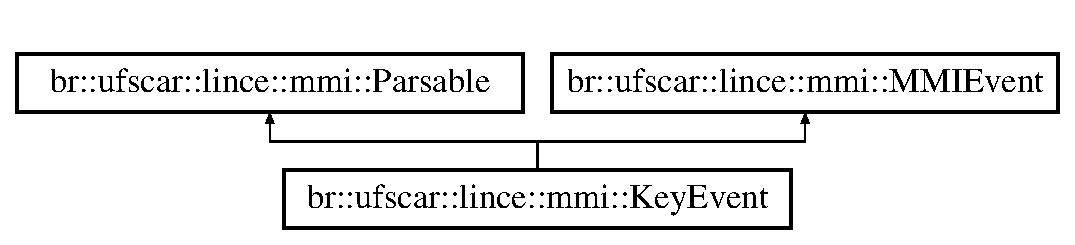
\includegraphics[height=2cm]{classbr_1_1ufscar_1_1lince_1_1mmi_1_1KeyEvent}
\end{center}
\end{figure}
\subsection*{Public Member Functions}
\begin{DoxyCompactItemize}
\item 
\hyperlink{classbr_1_1ufscar_1_1lince_1_1mmi_1_1KeyEvent_a6a6e61334c0e04dd3b43562dce2a107f}{KeyEvent} (string \hyperlink{classbr_1_1ufscar_1_1lince_1_1mmi_1_1MMIEvent_ab49d18c433659ed8e7dbdaa9004839d5}{deviceId}, string buttonId)
\begin{DoxyCompactList}\small\item\em Contrutor. \item\end{DoxyCompactList}\item 
virtual \hyperlink{classbr_1_1ufscar_1_1lince_1_1mmi_1_1KeyEvent_aadcb079c5602a9bc98dfdbc2f90bd500}{$\sim$KeyEvent} ()
\begin{DoxyCompactList}\small\item\em Destructor. \item\end{DoxyCompactList}\item 
string \hyperlink{classbr_1_1ufscar_1_1lince_1_1mmi_1_1KeyEvent_a4277d9938693821db5db50942f98fcb5}{getKeyId} ()
\begin{DoxyCompactList}\small\item\em This method returns the identificator of the key. \item\end{DoxyCompactList}\end{DoxyCompactItemize}
\subsection*{Friends}
\begin{DoxyCompactItemize}
\item 
class \hyperlink{classbr_1_1ufscar_1_1lince_1_1mmi_1_1KeyEvent_a2dd856aac914cf1b3eca999c688da31a}{KeyEventFactory}
\end{DoxyCompactItemize}


\subsection{Detailed Description}
This class represent a event of type key. Key Events are event generate when the user press a virtual or physical key or button. 

\subsection{Constructor \& Destructor Documentation}
\hypertarget{classbr_1_1ufscar_1_1lince_1_1mmi_1_1KeyEvent_a6a6e61334c0e04dd3b43562dce2a107f}{
\index{br::ufscar::lince::mmi::KeyEvent@{br::ufscar::lince::mmi::KeyEvent}!KeyEvent@{KeyEvent}}
\index{KeyEvent@{KeyEvent}!br::ufscar::lince::mmi::KeyEvent@{br::ufscar::lince::mmi::KeyEvent}}
\subsubsection[{KeyEvent}]{\setlength{\rightskip}{0pt plus 5cm}br::ufscar::lince::mmi::KeyEvent::KeyEvent (string {\em deviceId}, \/  string {\em buttonId})}}
\label{classbr_1_1ufscar_1_1lince_1_1mmi_1_1KeyEvent_a6a6e61334c0e04dd3b43562dce2a107f}


Contrutor. 


\begin{DoxyParams}{Parameters}
\item[{\em deviceId}]Name of the device that generate the event. \item[{\em eventType}]Type od the event. \end{DoxyParams}
\hypertarget{classbr_1_1ufscar_1_1lince_1_1mmi_1_1KeyEvent_aadcb079c5602a9bc98dfdbc2f90bd500}{
\index{br::ufscar::lince::mmi::KeyEvent@{br::ufscar::lince::mmi::KeyEvent}!$\sim$KeyEvent@{$\sim$KeyEvent}}
\index{$\sim$KeyEvent@{$\sim$KeyEvent}!br::ufscar::lince::mmi::KeyEvent@{br::ufscar::lince::mmi::KeyEvent}}
\subsubsection[{$\sim$KeyEvent}]{\setlength{\rightskip}{0pt plus 5cm}virtual br::ufscar::lince::mmi::KeyEvent::$\sim$KeyEvent ()\hspace{0.3cm}{\ttfamily  \mbox{[}virtual\mbox{]}}}}
\label{classbr_1_1ufscar_1_1lince_1_1mmi_1_1KeyEvent_aadcb079c5602a9bc98dfdbc2f90bd500}


Destructor. 



\subsection{Member Function Documentation}
\hypertarget{classbr_1_1ufscar_1_1lince_1_1mmi_1_1KeyEvent_a4277d9938693821db5db50942f98fcb5}{
\index{br::ufscar::lince::mmi::KeyEvent@{br::ufscar::lince::mmi::KeyEvent}!getKeyId@{getKeyId}}
\index{getKeyId@{getKeyId}!br::ufscar::lince::mmi::KeyEvent@{br::ufscar::lince::mmi::KeyEvent}}
\subsubsection[{getKeyId}]{\setlength{\rightskip}{0pt plus 5cm}string br::ufscar::lince::mmi::KeyEvent::getKeyId ()}}
\label{classbr_1_1ufscar_1_1lince_1_1mmi_1_1KeyEvent_a4277d9938693821db5db50942f98fcb5}


This method returns the identificator of the key. 

\begin{DoxyReturn}{Returns}
The key Id. 
\end{DoxyReturn}


\subsection{Friends And Related Function Documentation}
\hypertarget{classbr_1_1ufscar_1_1lince_1_1mmi_1_1KeyEvent_a2dd856aac914cf1b3eca999c688da31a}{
\index{br::ufscar::lince::mmi::KeyEvent@{br::ufscar::lince::mmi::KeyEvent}!KeyEventFactory@{KeyEventFactory}}
\index{KeyEventFactory@{KeyEventFactory}!br::ufscar::lince::mmi::KeyEvent@{br::ufscar::lince::mmi::KeyEvent}}
\subsubsection[{KeyEventFactory}]{\setlength{\rightskip}{0pt plus 5cm}friend class {\bf KeyEventFactory}\hspace{0.3cm}{\ttfamily  \mbox{[}friend\mbox{]}}}}
\label{classbr_1_1ufscar_1_1lince_1_1mmi_1_1KeyEvent_a2dd856aac914cf1b3eca999c688da31a}


The documentation for this class was generated from the following file:\begin{DoxyCompactItemize}
\item 
include/\hyperlink{KeyEvent_8h}{KeyEvent.h}\end{DoxyCompactItemize}

\hypertarget{classbr_1_1ufscar_1_1lince_1_1mmi_1_1KeyEventFactory}{
\section{br::ufscar::lince::mmi::KeyEventFactory Class Reference}
\label{classbr_1_1ufscar_1_1lince_1_1mmi_1_1KeyEventFactory}\index{br::ufscar::lince::mmi::KeyEventFactory@{br::ufscar::lince::mmi::KeyEventFactory}}
}


{\ttfamily \#include $<$KeyEventFactory.h$>$}

Inheritance diagram for br::ufscar::lince::mmi::KeyEventFactory:\begin{figure}[H]
\begin{center}
\leavevmode
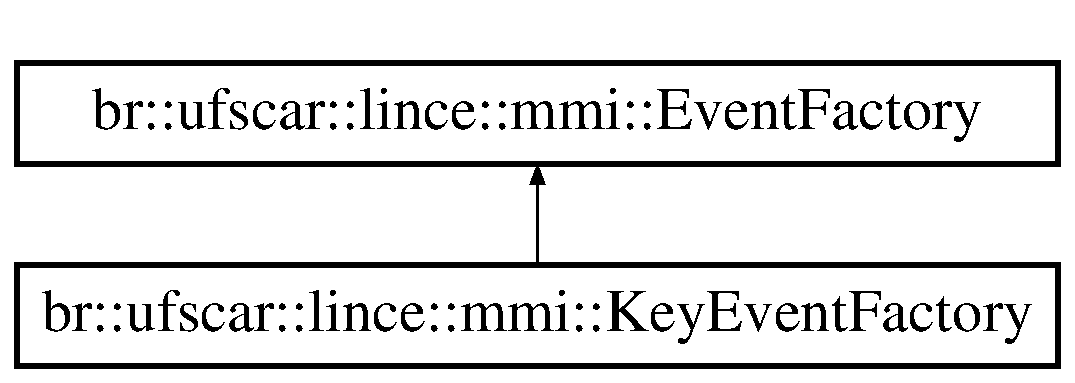
\includegraphics[height=2cm]{classbr_1_1ufscar_1_1lince_1_1mmi_1_1KeyEventFactory}
\end{center}
\end{figure}
\subsection*{Public Member Functions}
\begin{DoxyCompactItemize}
\item 
\hyperlink{classbr_1_1ufscar_1_1lince_1_1mmi_1_1KeyEventFactory_ab4158dc9066513f282ee670c3f98d716}{KeyEventFactory} ()
\item 
\hyperlink{classbr_1_1ufscar_1_1lince_1_1mmi_1_1KeyEventFactory_afbe72c85a1c20525aa60055b4de36f12}{$\sim$KeyEventFactory} ()
\item 
\hyperlink{classbr_1_1ufscar_1_1lince_1_1mmi_1_1MMIEvent}{MMIEvent} $\ast$ \hyperlink{classbr_1_1ufscar_1_1lince_1_1mmi_1_1KeyEventFactory_a838221bf5491967315a7475691e72103}{CreateEvent} (\hyperlink{structbr_1_1ufscar_1_1lince_1_1mmi_1_1XMLData}{XMLData} $\ast$data)
\end{DoxyCompactItemize}
\subsection*{Data Fields}
\begin{DoxyCompactItemize}
\item 
string \hyperlink{classbr_1_1ufscar_1_1lince_1_1mmi_1_1KeyEventFactory_a34a7fe739dd5ed97ee418df3c99c2e2c}{buttonId}
\end{DoxyCompactItemize}


\subsection{Constructor \& Destructor Documentation}
\hypertarget{classbr_1_1ufscar_1_1lince_1_1mmi_1_1KeyEventFactory_ab4158dc9066513f282ee670c3f98d716}{
\index{br::ufscar::lince::mmi::KeyEventFactory@{br::ufscar::lince::mmi::KeyEventFactory}!KeyEventFactory@{KeyEventFactory}}
\index{KeyEventFactory@{KeyEventFactory}!br::ufscar::lince::mmi::KeyEventFactory@{br::ufscar::lince::mmi::KeyEventFactory}}
\subsubsection[{KeyEventFactory}]{\setlength{\rightskip}{0pt plus 5cm}br::ufscar::lince::mmi::KeyEventFactory::KeyEventFactory ()}}
\label{classbr_1_1ufscar_1_1lince_1_1mmi_1_1KeyEventFactory_ab4158dc9066513f282ee670c3f98d716}
\hypertarget{classbr_1_1ufscar_1_1lince_1_1mmi_1_1KeyEventFactory_afbe72c85a1c20525aa60055b4de36f12}{
\index{br::ufscar::lince::mmi::KeyEventFactory@{br::ufscar::lince::mmi::KeyEventFactory}!$\sim$KeyEventFactory@{$\sim$KeyEventFactory}}
\index{$\sim$KeyEventFactory@{$\sim$KeyEventFactory}!br::ufscar::lince::mmi::KeyEventFactory@{br::ufscar::lince::mmi::KeyEventFactory}}
\subsubsection[{$\sim$KeyEventFactory}]{\setlength{\rightskip}{0pt plus 5cm}br::ufscar::lince::mmi::KeyEventFactory::$\sim$KeyEventFactory ()}}
\label{classbr_1_1ufscar_1_1lince_1_1mmi_1_1KeyEventFactory_afbe72c85a1c20525aa60055b4de36f12}


\subsection{Member Function Documentation}
\hypertarget{classbr_1_1ufscar_1_1lince_1_1mmi_1_1KeyEventFactory_a838221bf5491967315a7475691e72103}{
\index{br::ufscar::lince::mmi::KeyEventFactory@{br::ufscar::lince::mmi::KeyEventFactory}!CreateEvent@{CreateEvent}}
\index{CreateEvent@{CreateEvent}!br::ufscar::lince::mmi::KeyEventFactory@{br::ufscar::lince::mmi::KeyEventFactory}}
\subsubsection[{CreateEvent}]{\setlength{\rightskip}{0pt plus 5cm}{\bf MMIEvent}$\ast$ br::ufscar::lince::mmi::KeyEventFactory::CreateEvent ({\bf XMLData} $\ast$ {\em data})\hspace{0.3cm}{\ttfamily  \mbox{[}virtual\mbox{]}}}}
\label{classbr_1_1ufscar_1_1lince_1_1mmi_1_1KeyEventFactory_a838221bf5491967315a7475691e72103}


Implements \hyperlink{classbr_1_1ufscar_1_1lince_1_1mmi_1_1EventFactory_a19ad2165726a29a55c921f569764290b}{br::ufscar::lince::mmi::EventFactory}.



\subsection{Field Documentation}
\hypertarget{classbr_1_1ufscar_1_1lince_1_1mmi_1_1KeyEventFactory_a34a7fe739dd5ed97ee418df3c99c2e2c}{
\index{br::ufscar::lince::mmi::KeyEventFactory@{br::ufscar::lince::mmi::KeyEventFactory}!buttonId@{buttonId}}
\index{buttonId@{buttonId}!br::ufscar::lince::mmi::KeyEventFactory@{br::ufscar::lince::mmi::KeyEventFactory}}
\subsubsection[{buttonId}]{\setlength{\rightskip}{0pt plus 5cm}string {\bf br::ufscar::lince::mmi::KeyEventFactory::buttonId}}}
\label{classbr_1_1ufscar_1_1lince_1_1mmi_1_1KeyEventFactory_a34a7fe739dd5ed97ee418df3c99c2e2c}


The documentation for this class was generated from the following file:\begin{DoxyCompactItemize}
\item 
include/\hyperlink{KeyEventFactory_8h}{KeyEventFactory.h}\end{DoxyCompactItemize}

\hypertarget{structbr_1_1ufscar_1_1lince_1_1mmi_1_1LockedMultimodalAction}{
\section{br::ufscar::lince::mmi::LockedMultimodalAction Struct Reference}
\label{structbr_1_1ufscar_1_1lince_1_1mmi_1_1LockedMultimodalAction}\index{br::ufscar::lince::mmi::LockedMultimodalAction@{br::ufscar::lince::mmi::LockedMultimodalAction}}
}


{\ttfamily \#include $<$MMIManager.h$>$}

\subsection*{Data Fields}
\begin{DoxyCompactItemize}
\item 
::\hyperlink{classbr_1_1ufscar_1_1lince_1_1mmi_1_1MMIEventListener}{br::ufscar::lince::mmi::MMIEventListener} $\ast$ \hyperlink{structbr_1_1ufscar_1_1lince_1_1mmi_1_1LockedMultimodalAction_a290d66a9a01a9a81283860247eeaff10}{l}
\item 
::std::set$<$ string $>$ $\ast$ \hyperlink{structbr_1_1ufscar_1_1lince_1_1mmi_1_1LockedMultimodalAction_a3d8d1c55eacb7747c1e7d60fcb34a170}{eventTypes}
\item 
bool \hyperlink{structbr_1_1ufscar_1_1lince_1_1mmi_1_1LockedMultimodalAction_aaa42425599862561ea84845c72405b64}{isAdd}
\end{DoxyCompactItemize}


\subsection{Field Documentation}
\hypertarget{structbr_1_1ufscar_1_1lince_1_1mmi_1_1LockedMultimodalAction_a3d8d1c55eacb7747c1e7d60fcb34a170}{
\index{br::ufscar::lince::mmi::LockedMultimodalAction@{br::ufscar::lince::mmi::LockedMultimodalAction}!eventTypes@{eventTypes}}
\index{eventTypes@{eventTypes}!br::ufscar::lince::mmi::LockedMultimodalAction@{br::ufscar::lince::mmi::LockedMultimodalAction}}
\subsubsection[{eventTypes}]{\setlength{\rightskip}{0pt plus 5cm}::std::set$<$string$>$$\ast$ {\bf br::ufscar::lince::mmi::LockedMultimodalAction::eventTypes}}}
\label{structbr_1_1ufscar_1_1lince_1_1mmi_1_1LockedMultimodalAction_a3d8d1c55eacb7747c1e7d60fcb34a170}
\hypertarget{structbr_1_1ufscar_1_1lince_1_1mmi_1_1LockedMultimodalAction_aaa42425599862561ea84845c72405b64}{
\index{br::ufscar::lince::mmi::LockedMultimodalAction@{br::ufscar::lince::mmi::LockedMultimodalAction}!isAdd@{isAdd}}
\index{isAdd@{isAdd}!br::ufscar::lince::mmi::LockedMultimodalAction@{br::ufscar::lince::mmi::LockedMultimodalAction}}
\subsubsection[{isAdd}]{\setlength{\rightskip}{0pt plus 5cm}bool {\bf br::ufscar::lince::mmi::LockedMultimodalAction::isAdd}}}
\label{structbr_1_1ufscar_1_1lince_1_1mmi_1_1LockedMultimodalAction_aaa42425599862561ea84845c72405b64}
\hypertarget{structbr_1_1ufscar_1_1lince_1_1mmi_1_1LockedMultimodalAction_a290d66a9a01a9a81283860247eeaff10}{
\index{br::ufscar::lince::mmi::LockedMultimodalAction@{br::ufscar::lince::mmi::LockedMultimodalAction}!l@{l}}
\index{l@{l}!br::ufscar::lince::mmi::LockedMultimodalAction@{br::ufscar::lince::mmi::LockedMultimodalAction}}
\subsubsection[{l}]{\setlength{\rightskip}{0pt plus 5cm}::{\bf br::ufscar::lince::mmi::MMIEventListener}$\ast$ {\bf br::ufscar::lince::mmi::LockedMultimodalAction::l}}}
\label{structbr_1_1ufscar_1_1lince_1_1mmi_1_1LockedMultimodalAction_a290d66a9a01a9a81283860247eeaff10}


The documentation for this struct was generated from the following file:\begin{DoxyCompactItemize}
\item 
include/\hyperlink{MMIManager_8h}{MMIManager.h}\end{DoxyCompactItemize}

\hypertarget{classbr_1_1ufscar_1_1lince_1_1mmi_1_1MMIEvent}{
\section{br::ufscar::lince::mmi::MMIEvent Class Reference}
\label{classbr_1_1ufscar_1_1lince_1_1mmi_1_1MMIEvent}\index{br::ufscar::lince::mmi::MMIEvent@{br::ufscar::lince::mmi::MMIEvent}}
}


This class represent a generic Multimodal Event.  




{\ttfamily \#include $<$MMIEvent.h$>$}

Inheritance diagram for br::ufscar::lince::mmi::MMIEvent:\begin{figure}[H]
\begin{center}
\leavevmode
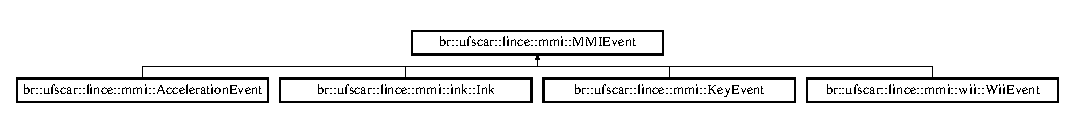
\includegraphics[height=1.14754cm]{classbr_1_1ufscar_1_1lince_1_1mmi_1_1MMIEvent}
\end{center}
\end{figure}
\subsection*{Public Member Functions}
\begin{DoxyCompactItemize}
\item 
\hyperlink{classbr_1_1ufscar_1_1lince_1_1mmi_1_1MMIEvent_ad2930762ec9b524bfe2824b2acc3b655}{MMIEvent} (string \hyperlink{classbr_1_1ufscar_1_1lince_1_1mmi_1_1MMIEvent_ab49d18c433659ed8e7dbdaa9004839d5}{deviceId}, string \hyperlink{classbr_1_1ufscar_1_1lince_1_1mmi_1_1MMIEvent_af26d77edf2187a0536c4365a3aaaf531}{eventType})
\begin{DoxyCompactList}\small\item\em Contrutor. \item\end{DoxyCompactList}\item 
virtual \hyperlink{classbr_1_1ufscar_1_1lince_1_1mmi_1_1MMIEvent_a657edd3701e56a3ab7901bcbe3f492ad}{$\sim$MMIEvent} ()
\begin{DoxyCompactList}\small\item\em Destructor. \item\end{DoxyCompactList}\item 
string \hyperlink{classbr_1_1ufscar_1_1lince_1_1mmi_1_1MMIEvent_a3bef1a44ba5335235b90dd89450d2b5c}{getDeviceId} ()
\begin{DoxyCompactList}\small\item\em This method returns the id of the device that generate the event. \item\end{DoxyCompactList}\item 
string \hyperlink{classbr_1_1ufscar_1_1lince_1_1mmi_1_1MMIEvent_a57aeaad0d4209139079bbc1314818c6a}{getEventType} ()
\begin{DoxyCompactList}\small\item\em This method returns the type of event. \item\end{DoxyCompactList}\end{DoxyCompactItemize}
\subsection*{Protected Attributes}
\begin{DoxyCompactItemize}
\item 
string \hyperlink{classbr_1_1ufscar_1_1lince_1_1mmi_1_1MMIEvent_ab49d18c433659ed8e7dbdaa9004839d5}{deviceId}
\item 
string \hyperlink{classbr_1_1ufscar_1_1lince_1_1mmi_1_1MMIEvent_af26d77edf2187a0536c4365a3aaaf531}{eventType}
\end{DoxyCompactItemize}


\subsection{Detailed Description}
This class represent a generic Multimodal Event. All multimodal event types must implement a specialization of this class. 

\subsection{Constructor \& Destructor Documentation}
\hypertarget{classbr_1_1ufscar_1_1lince_1_1mmi_1_1MMIEvent_ad2930762ec9b524bfe2824b2acc3b655}{
\index{br::ufscar::lince::mmi::MMIEvent@{br::ufscar::lince::mmi::MMIEvent}!MMIEvent@{MMIEvent}}
\index{MMIEvent@{MMIEvent}!br::ufscar::lince::mmi::MMIEvent@{br::ufscar::lince::mmi::MMIEvent}}
\subsubsection[{MMIEvent}]{\setlength{\rightskip}{0pt plus 5cm}br::ufscar::lince::mmi::MMIEvent::MMIEvent (string {\em deviceId}, \/  string {\em eventType})}}
\label{classbr_1_1ufscar_1_1lince_1_1mmi_1_1MMIEvent_ad2930762ec9b524bfe2824b2acc3b655}


Contrutor. 


\begin{DoxyParams}{Parameters}
\item[{\em deviceId}]Name of the device that generate the event. \item[{\em eventType}]Type od the event. \end{DoxyParams}
\hypertarget{classbr_1_1ufscar_1_1lince_1_1mmi_1_1MMIEvent_a657edd3701e56a3ab7901bcbe3f492ad}{
\index{br::ufscar::lince::mmi::MMIEvent@{br::ufscar::lince::mmi::MMIEvent}!$\sim$MMIEvent@{$\sim$MMIEvent}}
\index{$\sim$MMIEvent@{$\sim$MMIEvent}!br::ufscar::lince::mmi::MMIEvent@{br::ufscar::lince::mmi::MMIEvent}}
\subsubsection[{$\sim$MMIEvent}]{\setlength{\rightskip}{0pt plus 5cm}virtual br::ufscar::lince::mmi::MMIEvent::$\sim$MMIEvent ()\hspace{0.3cm}{\ttfamily  \mbox{[}virtual\mbox{]}}}}
\label{classbr_1_1ufscar_1_1lince_1_1mmi_1_1MMIEvent_a657edd3701e56a3ab7901bcbe3f492ad}


Destructor. 



\subsection{Member Function Documentation}
\hypertarget{classbr_1_1ufscar_1_1lince_1_1mmi_1_1MMIEvent_a3bef1a44ba5335235b90dd89450d2b5c}{
\index{br::ufscar::lince::mmi::MMIEvent@{br::ufscar::lince::mmi::MMIEvent}!getDeviceId@{getDeviceId}}
\index{getDeviceId@{getDeviceId}!br::ufscar::lince::mmi::MMIEvent@{br::ufscar::lince::mmi::MMIEvent}}
\subsubsection[{getDeviceId}]{\setlength{\rightskip}{0pt plus 5cm}string br::ufscar::lince::mmi::MMIEvent::getDeviceId ()}}
\label{classbr_1_1ufscar_1_1lince_1_1mmi_1_1MMIEvent_a3bef1a44ba5335235b90dd89450d2b5c}


This method returns the id of the device that generate the event. 

\begin{DoxyReturn}{Returns}
Device id. 
\end{DoxyReturn}
\hypertarget{classbr_1_1ufscar_1_1lince_1_1mmi_1_1MMIEvent_a57aeaad0d4209139079bbc1314818c6a}{
\index{br::ufscar::lince::mmi::MMIEvent@{br::ufscar::lince::mmi::MMIEvent}!getEventType@{getEventType}}
\index{getEventType@{getEventType}!br::ufscar::lince::mmi::MMIEvent@{br::ufscar::lince::mmi::MMIEvent}}
\subsubsection[{getEventType}]{\setlength{\rightskip}{0pt plus 5cm}string br::ufscar::lince::mmi::MMIEvent::getEventType ()}}
\label{classbr_1_1ufscar_1_1lince_1_1mmi_1_1MMIEvent_a57aeaad0d4209139079bbc1314818c6a}


This method returns the type of event. 

\begin{DoxyReturn}{Returns}
Event type. 
\end{DoxyReturn}


\subsection{Field Documentation}
\hypertarget{classbr_1_1ufscar_1_1lince_1_1mmi_1_1MMIEvent_ab49d18c433659ed8e7dbdaa9004839d5}{
\index{br::ufscar::lince::mmi::MMIEvent@{br::ufscar::lince::mmi::MMIEvent}!deviceId@{deviceId}}
\index{deviceId@{deviceId}!br::ufscar::lince::mmi::MMIEvent@{br::ufscar::lince::mmi::MMIEvent}}
\subsubsection[{deviceId}]{\setlength{\rightskip}{0pt plus 5cm}string {\bf br::ufscar::lince::mmi::MMIEvent::deviceId}\hspace{0.3cm}{\ttfamily  \mbox{[}protected\mbox{]}}}}
\label{classbr_1_1ufscar_1_1lince_1_1mmi_1_1MMIEvent_ab49d18c433659ed8e7dbdaa9004839d5}
\hypertarget{classbr_1_1ufscar_1_1lince_1_1mmi_1_1MMIEvent_af26d77edf2187a0536c4365a3aaaf531}{
\index{br::ufscar::lince::mmi::MMIEvent@{br::ufscar::lince::mmi::MMIEvent}!eventType@{eventType}}
\index{eventType@{eventType}!br::ufscar::lince::mmi::MMIEvent@{br::ufscar::lince::mmi::MMIEvent}}
\subsubsection[{eventType}]{\setlength{\rightskip}{0pt plus 5cm}string {\bf br::ufscar::lince::mmi::MMIEvent::eventType}\hspace{0.3cm}{\ttfamily  \mbox{[}protected\mbox{]}}}}
\label{classbr_1_1ufscar_1_1lince_1_1mmi_1_1MMIEvent_af26d77edf2187a0536c4365a3aaaf531}


The documentation for this class was generated from the following file:\begin{DoxyCompactItemize}
\item 
include/\hyperlink{MMIEvent_8h}{MMIEvent.h}\end{DoxyCompactItemize}

\hypertarget{classbr_1_1ufscar_1_1lince_1_1mmi_1_1MMIEventListener}{
\section{br::ufscar::lince::mmi::MMIEventListener Class Reference}
\label{classbr_1_1ufscar_1_1lince_1_1mmi_1_1MMIEventListener}\index{br::ufscar::lince::mmi::MMIEventListener@{br::ufscar::lince::mmi::MMIEventListener}}
}


This abstract class represents a instance that can listen to MultimodalE vents.  




{\ttfamily \#include $<$MMIEventListener.h$>$}

\subsection*{Public Member Functions}
\begin{DoxyCompactItemize}
\item 
virtual \hyperlink{classbr_1_1ufscar_1_1lince_1_1mmi_1_1MMIEventListener_a49dad88c24782f8d123289aea725e73e}{$\sim$MMIEventListener} ()
\begin{DoxyCompactList}\small\item\em Generic Destructor. \item\end{DoxyCompactList}\item 
virtual bool \hyperlink{classbr_1_1ufscar_1_1lince_1_1mmi_1_1MMIEventListener_a2b7631e7ed09e2235b021fb2b5ba3b66}{receiveEvent} (\hyperlink{classbr_1_1ufscar_1_1lince_1_1mmi_1_1MMIEvent}{MMIEvent} $\ast$event)=0
\begin{DoxyCompactList}\small\item\em This method receives multimodal events when they occurs. \item\end{DoxyCompactList}\end{DoxyCompactItemize}


\subsection{Detailed Description}
This abstract class represents a instance that can listen to MultimodalE vents. Any application that wish be notified when a Multimodal Events occurs must implement this class and register a instance in the \hyperlink{classbr_1_1ufscar_1_1lince_1_1mmi_1_1MMIManager}{MMIManager}. Everytime a Multimodal Event occurs, the methods receiveEvent of that instance will be called by the MIIManager. 

\subsection{Constructor \& Destructor Documentation}
\hypertarget{classbr_1_1ufscar_1_1lince_1_1mmi_1_1MMIEventListener_a49dad88c24782f8d123289aea725e73e}{
\index{br::ufscar::lince::mmi::MMIEventListener@{br::ufscar::lince::mmi::MMIEventListener}!$\sim$MMIEventListener@{$\sim$MMIEventListener}}
\index{$\sim$MMIEventListener@{$\sim$MMIEventListener}!br::ufscar::lince::mmi::MMIEventListener@{br::ufscar::lince::mmi::MMIEventListener}}
\subsubsection[{$\sim$MMIEventListener}]{\setlength{\rightskip}{0pt plus 5cm}virtual br::ufscar::lince::mmi::MMIEventListener::$\sim$MMIEventListener ()\hspace{0.3cm}{\ttfamily  \mbox{[}inline, virtual\mbox{]}}}}
\label{classbr_1_1ufscar_1_1lince_1_1mmi_1_1MMIEventListener_a49dad88c24782f8d123289aea725e73e}


Generic Destructor. 



\subsection{Member Function Documentation}
\hypertarget{classbr_1_1ufscar_1_1lince_1_1mmi_1_1MMIEventListener_a2b7631e7ed09e2235b021fb2b5ba3b66}{
\index{br::ufscar::lince::mmi::MMIEventListener@{br::ufscar::lince::mmi::MMIEventListener}!receiveEvent@{receiveEvent}}
\index{receiveEvent@{receiveEvent}!br::ufscar::lince::mmi::MMIEventListener@{br::ufscar::lince::mmi::MMIEventListener}}
\subsubsection[{receiveEvent}]{\setlength{\rightskip}{0pt plus 5cm}virtual bool br::ufscar::lince::mmi::MMIEventListener::receiveEvent ({\bf MMIEvent} $\ast$ {\em event})\hspace{0.3cm}{\ttfamily  \mbox{[}pure virtual\mbox{]}}}}
\label{classbr_1_1ufscar_1_1lince_1_1mmi_1_1MMIEventListener_a2b7631e7ed09e2235b021fb2b5ba3b66}


This method receives multimodal events when they occurs. 


\begin{DoxyParams}{Parameters}
\item[{\em event}]The multimodal event that occurs. \end{DoxyParams}


The documentation for this class was generated from the following file:\begin{DoxyCompactItemize}
\item 
include/\hyperlink{MMIEventListener_8h}{MMIEventListener.h}\end{DoxyCompactItemize}

\hypertarget{classbr_1_1ufscar_1_1lince_1_1mmi_1_1MMIManager}{
\section{br::ufscar::lince::mmi::MMIManager Class Reference}
\label{classbr_1_1ufscar_1_1lince_1_1mmi_1_1MMIManager}\index{br::ufscar::lince::mmi::MMIManager@{br::ufscar::lince::mmi::MMIManager}}
}


This class control the multimodal interactions.  




{\ttfamily \#include $<$MMIManager.h$>$}

\subsection*{Public Member Functions}
\begin{DoxyCompactItemize}
\item 
virtual void \hyperlink{classbr_1_1ufscar_1_1lince_1_1mmi_1_1MMIManager_a2e9b5dd15d1c2bd1f34192193c840365}{release} ()
\begin{DoxyCompactList}\small\item\em This method release the internal variabels of the \hyperlink{classbr_1_1ufscar_1_1lince_1_1mmi_1_1MMIManager}{MMIManager}. \item\end{DoxyCompactList}\item 
void \hyperlink{classbr_1_1ufscar_1_1lince_1_1mmi_1_1MMIManager_a140389a1e17ba07406d79a427039ab1b}{postEvent} (\hyperlink{classbr_1_1ufscar_1_1lince_1_1mmi_1_1MMIEvent}{MMIEvent} $\ast$event)
\begin{DoxyCompactList}\small\item\em This method allow a device driver post Multimodal events generateds. \item\end{DoxyCompactList}\item 
void \hyperlink{classbr_1_1ufscar_1_1lince_1_1mmi_1_1MMIManager_ac9208d28d50a1f9e727c34f79d7e23f0}{postXMLEvent} (\hyperlink{structbr_1_1ufscar_1_1lince_1_1mmi_1_1XMLData}{XMLData} $\ast$event)
\begin{DoxyCompactList}\small\item\em This method allow the network services post XML Documents that represents a Multimodal Event. \item\end{DoxyCompactList}\item 
void \hyperlink{classbr_1_1ufscar_1_1lince_1_1mmi_1_1MMIManager_a724f0254692c6dddf2adea7e87286bf5}{registerDevice} (\hyperlink{classbr_1_1ufscar_1_1lince_1_1mmi_1_1IDeviceComm}{IDeviceComm} $\ast$device, string deviceId)
\begin{DoxyCompactList}\small\item\em This method allows devices register themselves in the \hyperlink{classbr_1_1ufscar_1_1lince_1_1mmi_1_1MMIManager}{MMIManager}. \item\end{DoxyCompactList}\item 
void \hyperlink{classbr_1_1ufscar_1_1lince_1_1mmi_1_1MMIManager_a67dfd0985484c895eb0081521835dd7b}{unregisterDevice} (string deviceId)
\begin{DoxyCompactList}\small\item\em This method allow devices unregister. \item\end{DoxyCompactList}\item 
void \hyperlink{classbr_1_1ufscar_1_1lince_1_1mmi_1_1MMIManager_a6cd07df71e304c7257c91ce145ada8f5}{addEventListener} (\hyperlink{classbr_1_1ufscar_1_1lince_1_1mmi_1_1MMIEventListener}{MMIEventListener} $\ast$listener, set$<$ string $>$ $\ast$eventTypes)
\begin{DoxyCompactList}\small\item\em This method allow the registration of objects that wish receive multimodal events. \item\end{DoxyCompactList}\item 
void \hyperlink{classbr_1_1ufscar_1_1lince_1_1mmi_1_1MMIManager_af301df4426b81e014b718a0a9cfb398f}{removeEventListener} (\hyperlink{classbr_1_1ufscar_1_1lince_1_1mmi_1_1MMIEventListener}{MMIEventListener} $\ast$listener)
\begin{DoxyCompactList}\small\item\em This method remove objets of the list of multimodal event listeners. \item\end{DoxyCompactList}\item 
vector$<$ string $>$ $\ast$ \hyperlink{classbr_1_1ufscar_1_1lince_1_1mmi_1_1MMIManager_a10ea6c549e2381748e8f6dbab2181942}{getDevicesName} ()
\begin{DoxyCompactList}\small\item\em This method returns the id of all devices registred. \item\end{DoxyCompactList}\item 
void \hyperlink{classbr_1_1ufscar_1_1lince_1_1mmi_1_1MMIManager_afaf755202a19c63ec903ff1d70362126}{callDeviceService} (string deviceId, vector$<$ string $>$ $\ast$args)
\begin{DoxyCompactList}\small\item\em This method allow applications send message to devices. \item\end{DoxyCompactList}\item 
virtual void \hyperlink{classbr_1_1ufscar_1_1lince_1_1mmi_1_1MMIManager_a1b1bf42389517969c28bfc0062e05f91}{waitForUnlockCondition} ()
\end{DoxyCompactItemize}
\subsection*{Static Public Member Functions}
\begin{DoxyCompactItemize}
\item 
static \hyperlink{classbr_1_1ufscar_1_1lince_1_1mmi_1_1MMIManager}{MMIManager} $\ast$ \hyperlink{classbr_1_1ufscar_1_1lince_1_1mmi_1_1MMIManager_ab14c6d4285139f01cc5d67a5e650b9c4}{getInstance} ()
\begin{DoxyCompactList}\small\item\em This method allow getting the unique instance of \hyperlink{classbr_1_1ufscar_1_1lince_1_1mmi_1_1MMIManager}{MMIManager}. \item\end{DoxyCompactList}\end{DoxyCompactItemize}


\subsection{Detailed Description}
This class control the multimodal interactions. The application must register themselves in the instance of \hyperlink{classbr_1_1ufscar_1_1lince_1_1mmi_1_1MMIManager}{MMIManager} to receive the MMIEvents that occurs. 

\subsection{Member Function Documentation}
\hypertarget{classbr_1_1ufscar_1_1lince_1_1mmi_1_1MMIManager_a6cd07df71e304c7257c91ce145ada8f5}{
\index{br::ufscar::lince::mmi::MMIManager@{br::ufscar::lince::mmi::MMIManager}!addEventListener@{addEventListener}}
\index{addEventListener@{addEventListener}!br::ufscar::lince::mmi::MMIManager@{br::ufscar::lince::mmi::MMIManager}}
\subsubsection[{addEventListener}]{\setlength{\rightskip}{0pt plus 5cm}void br::ufscar::lince::mmi::MMIManager::addEventListener ({\bf MMIEventListener} $\ast$ {\em listener}, \/  set$<$ string $>$ $\ast$ {\em eventTypes})}}
\label{classbr_1_1ufscar_1_1lince_1_1mmi_1_1MMIManager_a6cd07df71e304c7257c91ce145ada8f5}


This method allow the registration of objects that wish receive multimodal events. 


\begin{DoxyParams}{Parameters}
\item[{\em The}]instance of object that wish receive multimodal events \item[{\em eventTypes}]a set of eventTypes that the object wish receive. \end{DoxyParams}
\hypertarget{classbr_1_1ufscar_1_1lince_1_1mmi_1_1MMIManager_afaf755202a19c63ec903ff1d70362126}{
\index{br::ufscar::lince::mmi::MMIManager@{br::ufscar::lince::mmi::MMIManager}!callDeviceService@{callDeviceService}}
\index{callDeviceService@{callDeviceService}!br::ufscar::lince::mmi::MMIManager@{br::ufscar::lince::mmi::MMIManager}}
\subsubsection[{callDeviceService}]{\setlength{\rightskip}{0pt plus 5cm}void br::ufscar::lince::mmi::MMIManager::callDeviceService (string {\em deviceId}, \/  vector$<$ string $>$ $\ast$ {\em args})}}
\label{classbr_1_1ufscar_1_1lince_1_1mmi_1_1MMIManager_afaf755202a19c63ec903ff1d70362126}


This method allow applications send message to devices. 


\begin{DoxyParams}{Parameters}
\item[{\em deviceId}]The deviceId that will receive the message. \item[{\em args}]A vector with the message that will be send. \end{DoxyParams}
\hypertarget{classbr_1_1ufscar_1_1lince_1_1mmi_1_1MMIManager_a10ea6c549e2381748e8f6dbab2181942}{
\index{br::ufscar::lince::mmi::MMIManager@{br::ufscar::lince::mmi::MMIManager}!getDevicesName@{getDevicesName}}
\index{getDevicesName@{getDevicesName}!br::ufscar::lince::mmi::MMIManager@{br::ufscar::lince::mmi::MMIManager}}
\subsubsection[{getDevicesName}]{\setlength{\rightskip}{0pt plus 5cm}vector$<$string$>$$\ast$ br::ufscar::lince::mmi::MMIManager::getDevicesName ()}}
\label{classbr_1_1ufscar_1_1lince_1_1mmi_1_1MMIManager_a10ea6c549e2381748e8f6dbab2181942}


This method returns the id of all devices registred. 


\begin{DoxyParams}{Parameters}
\item[{\em A}]Vector with the id of all devices. \end{DoxyParams}
\hypertarget{classbr_1_1ufscar_1_1lince_1_1mmi_1_1MMIManager_ab14c6d4285139f01cc5d67a5e650b9c4}{
\index{br::ufscar::lince::mmi::MMIManager@{br::ufscar::lince::mmi::MMIManager}!getInstance@{getInstance}}
\index{getInstance@{getInstance}!br::ufscar::lince::mmi::MMIManager@{br::ufscar::lince::mmi::MMIManager}}
\subsubsection[{getInstance}]{\setlength{\rightskip}{0pt plus 5cm}static {\bf MMIManager}$\ast$ br::ufscar::lince::mmi::MMIManager::getInstance ()\hspace{0.3cm}{\ttfamily  \mbox{[}static\mbox{]}}}}
\label{classbr_1_1ufscar_1_1lince_1_1mmi_1_1MMIManager_ab14c6d4285139f01cc5d67a5e650b9c4}


This method allow getting the unique instance of \hyperlink{classbr_1_1ufscar_1_1lince_1_1mmi_1_1MMIManager}{MMIManager}. 


\begin{DoxyParams}{Parameters}
\item[{\em Unique}]instance of \hyperlink{classbr_1_1ufscar_1_1lince_1_1mmi_1_1MMIManager}{MMIManager}. \end{DoxyParams}
\hypertarget{classbr_1_1ufscar_1_1lince_1_1mmi_1_1MMIManager_a140389a1e17ba07406d79a427039ab1b}{
\index{br::ufscar::lince::mmi::MMIManager@{br::ufscar::lince::mmi::MMIManager}!postEvent@{postEvent}}
\index{postEvent@{postEvent}!br::ufscar::lince::mmi::MMIManager@{br::ufscar::lince::mmi::MMIManager}}
\subsubsection[{postEvent}]{\setlength{\rightskip}{0pt plus 5cm}void br::ufscar::lince::mmi::MMIManager::postEvent ({\bf MMIEvent} $\ast$ {\em event})}}
\label{classbr_1_1ufscar_1_1lince_1_1mmi_1_1MMIManager_a140389a1e17ba07406d79a427039ab1b}


This method allow a device driver post Multimodal events generateds. 


\begin{DoxyParams}{Parameters}
\item[{\em event}]The Multimodal event. \end{DoxyParams}
\hypertarget{classbr_1_1ufscar_1_1lince_1_1mmi_1_1MMIManager_ac9208d28d50a1f9e727c34f79d7e23f0}{
\index{br::ufscar::lince::mmi::MMIManager@{br::ufscar::lince::mmi::MMIManager}!postXMLEvent@{postXMLEvent}}
\index{postXMLEvent@{postXMLEvent}!br::ufscar::lince::mmi::MMIManager@{br::ufscar::lince::mmi::MMIManager}}
\subsubsection[{postXMLEvent}]{\setlength{\rightskip}{0pt plus 5cm}void br::ufscar::lince::mmi::MMIManager::postXMLEvent ({\bf XMLData} $\ast$ {\em event})}}
\label{classbr_1_1ufscar_1_1lince_1_1mmi_1_1MMIManager_ac9208d28d50a1f9e727c34f79d7e23f0}


This method allow the network services post XML Documents that represents a Multimodal Event. 

The XML Documents will be parsed and reposted as a instance of \hyperlink{classbr_1_1ufscar_1_1lince_1_1mmi_1_1MMIEvent}{MMIEvent}. 
\begin{DoxyParams}{Parameters}
\item[{\em event}]The XML Document Representation. \end{DoxyParams}
\hypertarget{classbr_1_1ufscar_1_1lince_1_1mmi_1_1MMIManager_a724f0254692c6dddf2adea7e87286bf5}{
\index{br::ufscar::lince::mmi::MMIManager@{br::ufscar::lince::mmi::MMIManager}!registerDevice@{registerDevice}}
\index{registerDevice@{registerDevice}!br::ufscar::lince::mmi::MMIManager@{br::ufscar::lince::mmi::MMIManager}}
\subsubsection[{registerDevice}]{\setlength{\rightskip}{0pt plus 5cm}void br::ufscar::lince::mmi::MMIManager::registerDevice ({\bf IDeviceComm} $\ast$ {\em device}, \/  string {\em deviceId})}}
\label{classbr_1_1ufscar_1_1lince_1_1mmi_1_1MMIManager_a724f0254692c6dddf2adea7e87286bf5}


This method allows devices register themselves in the \hyperlink{classbr_1_1ufscar_1_1lince_1_1mmi_1_1MMIManager}{MMIManager}. 


\begin{DoxyParams}{Parameters}
\item[{\em device}]The Device instance representation. \item[{\em deviceId}]The identification of the device. \end{DoxyParams}
\hypertarget{classbr_1_1ufscar_1_1lince_1_1mmi_1_1MMIManager_a2e9b5dd15d1c2bd1f34192193c840365}{
\index{br::ufscar::lince::mmi::MMIManager@{br::ufscar::lince::mmi::MMIManager}!release@{release}}
\index{release@{release}!br::ufscar::lince::mmi::MMIManager@{br::ufscar::lince::mmi::MMIManager}}
\subsubsection[{release}]{\setlength{\rightskip}{0pt plus 5cm}virtual void br::ufscar::lince::mmi::MMIManager::release ()\hspace{0.3cm}{\ttfamily  \mbox{[}virtual\mbox{]}}}}
\label{classbr_1_1ufscar_1_1lince_1_1mmi_1_1MMIManager_a2e9b5dd15d1c2bd1f34192193c840365}


This method release the internal variabels of the \hyperlink{classbr_1_1ufscar_1_1lince_1_1mmi_1_1MMIManager}{MMIManager}. 

\hypertarget{classbr_1_1ufscar_1_1lince_1_1mmi_1_1MMIManager_af301df4426b81e014b718a0a9cfb398f}{
\index{br::ufscar::lince::mmi::MMIManager@{br::ufscar::lince::mmi::MMIManager}!removeEventListener@{removeEventListener}}
\index{removeEventListener@{removeEventListener}!br::ufscar::lince::mmi::MMIManager@{br::ufscar::lince::mmi::MMIManager}}
\subsubsection[{removeEventListener}]{\setlength{\rightskip}{0pt plus 5cm}void br::ufscar::lince::mmi::MMIManager::removeEventListener ({\bf MMIEventListener} $\ast$ {\em listener})}}
\label{classbr_1_1ufscar_1_1lince_1_1mmi_1_1MMIManager_af301df4426b81e014b718a0a9cfb398f}


This method remove objets of the list of multimodal event listeners. 


\begin{DoxyParams}{Parameters}
\item[{\em listener}]The object that will be removed of the list. \end{DoxyParams}
\hypertarget{classbr_1_1ufscar_1_1lince_1_1mmi_1_1MMIManager_a67dfd0985484c895eb0081521835dd7b}{
\index{br::ufscar::lince::mmi::MMIManager@{br::ufscar::lince::mmi::MMIManager}!unregisterDevice@{unregisterDevice}}
\index{unregisterDevice@{unregisterDevice}!br::ufscar::lince::mmi::MMIManager@{br::ufscar::lince::mmi::MMIManager}}
\subsubsection[{unregisterDevice}]{\setlength{\rightskip}{0pt plus 5cm}void br::ufscar::lince::mmi::MMIManager::unregisterDevice (string {\em deviceId})}}
\label{classbr_1_1ufscar_1_1lince_1_1mmi_1_1MMIManager_a67dfd0985484c895eb0081521835dd7b}


This method allow devices unregister. 


\begin{DoxyParams}{Parameters}
\item[{\em deviceId}]The deviceId that will be unregistred. \end{DoxyParams}
\hypertarget{classbr_1_1ufscar_1_1lince_1_1mmi_1_1MMIManager_a1b1bf42389517969c28bfc0062e05f91}{
\index{br::ufscar::lince::mmi::MMIManager@{br::ufscar::lince::mmi::MMIManager}!waitForUnlockCondition@{waitForUnlockCondition}}
\index{waitForUnlockCondition@{waitForUnlockCondition}!br::ufscar::lince::mmi::MMIManager@{br::ufscar::lince::mmi::MMIManager}}
\subsubsection[{waitForUnlockCondition}]{\setlength{\rightskip}{0pt plus 5cm}virtual void br::ufscar::lince::mmi::MMIManager::waitForUnlockCondition ()\hspace{0.3cm}{\ttfamily  \mbox{[}virtual\mbox{]}}}}
\label{classbr_1_1ufscar_1_1lince_1_1mmi_1_1MMIManager_a1b1bf42389517969c28bfc0062e05f91}


The documentation for this class was generated from the following file:\begin{DoxyCompactItemize}
\item 
include/\hyperlink{MMIManager_8h}{MMIManager.h}\end{DoxyCompactItemize}

\hypertarget{classbr_1_1ufscar_1_1lince_1_1mmi_1_1upnp_1_1MMIService}{
\section{br::ufscar::lince::mmi::upnp::MMIService Class Reference}
\label{classbr_1_1ufscar_1_1lince_1_1mmi_1_1upnp_1_1MMIService}\index{br::ufscar::lince::mmi::upnp::MMIService@{br::ufscar::lince::mmi::upnp::MMIService}}
}


Esta classe representa um dispositivo e seu serviços.  




{\ttfamily \#include $<$MMIService.h$>$}

\subsection*{Public Member Functions}
\begin{DoxyCompactItemize}
\item 
bool \hyperlink{classbr_1_1ufscar_1_1lince_1_1mmi_1_1upnp_1_1MMIService_a34c70b44f4b7491dc2e9a398423ef974}{start} ()
\begin{DoxyCompactList}\small\item\em Inicia os serviços. \item\end{DoxyCompactList}\item 
bool \hyperlink{classbr_1_1ufscar_1_1lince_1_1mmi_1_1upnp_1_1MMIService_a0687c9dbf5bbbaa2b490e19bb88a1a51}{stop} ()
\begin{DoxyCompactList}\small\item\em Pára os serviços. \item\end{DoxyCompactList}\item 
void \hyperlink{classbr_1_1ufscar_1_1lince_1_1mmi_1_1upnp_1_1MMIService_a0163a8a90ce5a43daad480795d323f5c}{initializeUPnPStateVariables} ()
\begin{DoxyCompactList}\small\item\em Inicializa as variáveis de estado necessárias ao funcionamento do serviço. \item\end{DoxyCompactList}\item 
UPnPService $\ast$ \hyperlink{classbr_1_1ufscar_1_1lince_1_1mmi_1_1upnp_1_1MMIService_aadd21fd9892177f42ca1e002b5dc6432}{getService} ()
\begin{DoxyCompactList}\small\item\em Retorna a instância do serviço UPnP. \item\end{DoxyCompactList}\item 
bool \hyperlink{classbr_1_1ufscar_1_1lince_1_1mmi_1_1upnp_1_1MMIService_a7fb929d5234cabe8bccffcbace4a97dc}{actionRequest} (UPnPAction $\ast$action)
\begin{DoxyCompactList}\small\item\em Recebe solicitações de ações a serem executadas. \item\end{DoxyCompactList}\item 
bool \hyperlink{classbr_1_1ufscar_1_1lince_1_1mmi_1_1upnp_1_1MMIService_a1e6559d7dbe7372d8f60e451ac157935}{variableRequest} (UPnPStateVariable $\ast$stateVar)
\begin{DoxyCompactList}\small\item\em Envia o estado atual de uma variável do serviço. \item\end{DoxyCompactList}\item 
bool \hyperlink{classbr_1_1ufscar_1_1lince_1_1mmi_1_1upnp_1_1MMIService_abd5a9ef1a311388d61cfe7c1a8380f56}{actionPostEvent} (UPnPAction $\ast$action)
\begin{DoxyCompactList}\small\item\em Recebe uma mensagem (texto) de um dispositivo remoto. \item\end{DoxyCompactList}\end{DoxyCompactItemize}
\subsection*{Static Public Member Functions}
\begin{DoxyCompactItemize}
\item 
static \hyperlink{classbr_1_1ufscar_1_1lince_1_1mmi_1_1upnp_1_1MMIService}{MMIService} $\ast$ \hyperlink{classbr_1_1ufscar_1_1lince_1_1mmi_1_1upnp_1_1MMIService_a369cf8700f091154c446028e26c65cce}{getInstance} ()
\begin{DoxyCompactList}\small\item\em Acessa a instância única. \item\end{DoxyCompactList}\end{DoxyCompactItemize}
\subsection*{Protected Member Functions}
\begin{DoxyCompactItemize}
\item 
\hyperlink{classbr_1_1ufscar_1_1lince_1_1mmi_1_1upnp_1_1MMIService_a02cbbb28a8831c5c5d535fc76111eb96}{MMIService} ()
\begin{DoxyCompactList}\small\item\em Construtor. \item\end{DoxyCompactList}\item 
\hyperlink{classbr_1_1ufscar_1_1lince_1_1mmi_1_1upnp_1_1MMIService_a549825fd03af5db240df7435e66fe9fb}{$\sim$MMIService} ()
\begin{DoxyCompactList}\small\item\em Destrutor. \item\end{DoxyCompactList}\end{DoxyCompactItemize}


\subsection{Detailed Description}
Esta classe representa um dispositivo e seu serviços. Cada dispositivo possui sua descrição e os serviços que disponibiliza. Recebe as chamadas de métodos (ações), faz o tratamento e devolve o resultado para o dispositivo que o invocou. 

\subsection{Constructor \& Destructor Documentation}
\hypertarget{classbr_1_1ufscar_1_1lince_1_1mmi_1_1upnp_1_1MMIService_a02cbbb28a8831c5c5d535fc76111eb96}{
\index{br::ufscar::lince::mmi::upnp::MMIService@{br::ufscar::lince::mmi::upnp::MMIService}!MMIService@{MMIService}}
\index{MMIService@{MMIService}!br::ufscar::lince::mmi::upnp::MMIService@{br::ufscar::lince::mmi::upnp::MMIService}}
\subsubsection[{MMIService}]{\setlength{\rightskip}{0pt plus 5cm}br::ufscar::lince::mmi::upnp::MMIService::MMIService ()\hspace{0.3cm}{\ttfamily  \mbox{[}protected\mbox{]}}}}
\label{classbr_1_1ufscar_1_1lince_1_1mmi_1_1upnp_1_1MMIService_a02cbbb28a8831c5c5d535fc76111eb96}


Construtor. 

\hypertarget{classbr_1_1ufscar_1_1lince_1_1mmi_1_1upnp_1_1MMIService_a549825fd03af5db240df7435e66fe9fb}{
\index{br::ufscar::lince::mmi::upnp::MMIService@{br::ufscar::lince::mmi::upnp::MMIService}!$\sim$MMIService@{$\sim$MMIService}}
\index{$\sim$MMIService@{$\sim$MMIService}!br::ufscar::lince::mmi::upnp::MMIService@{br::ufscar::lince::mmi::upnp::MMIService}}
\subsubsection[{$\sim$MMIService}]{\setlength{\rightskip}{0pt plus 5cm}br::ufscar::lince::mmi::upnp::MMIService::$\sim$MMIService ()\hspace{0.3cm}{\ttfamily  \mbox{[}protected\mbox{]}}}}
\label{classbr_1_1ufscar_1_1lince_1_1mmi_1_1upnp_1_1MMIService_a549825fd03af5db240df7435e66fe9fb}


Destrutor. 



\subsection{Member Function Documentation}
\hypertarget{classbr_1_1ufscar_1_1lince_1_1mmi_1_1upnp_1_1MMIService_abd5a9ef1a311388d61cfe7c1a8380f56}{
\index{br::ufscar::lince::mmi::upnp::MMIService@{br::ufscar::lince::mmi::upnp::MMIService}!actionPostEvent@{actionPostEvent}}
\index{actionPostEvent@{actionPostEvent}!br::ufscar::lince::mmi::upnp::MMIService@{br::ufscar::lince::mmi::upnp::MMIService}}
\subsubsection[{actionPostEvent}]{\setlength{\rightskip}{0pt plus 5cm}bool br::ufscar::lince::mmi::upnp::MMIService::actionPostEvent (UPnPAction $\ast$ {\em action})}}
\label{classbr_1_1ufscar_1_1lince_1_1mmi_1_1upnp_1_1MMIService_abd5a9ef1a311388d61cfe7c1a8380f56}


Recebe uma mensagem (texto) de um dispositivo remoto. 


\begin{DoxyParams}{Parameters}
\item[{\em action}]ação a ser executada. \end{DoxyParams}
\begin{DoxyReturn}{Returns}
true, caso a ação seja executada com sucesso, ou false, caso contrário. 
\end{DoxyReturn}
\hypertarget{classbr_1_1ufscar_1_1lince_1_1mmi_1_1upnp_1_1MMIService_a7fb929d5234cabe8bccffcbace4a97dc}{
\index{br::ufscar::lince::mmi::upnp::MMIService@{br::ufscar::lince::mmi::upnp::MMIService}!actionRequest@{actionRequest}}
\index{actionRequest@{actionRequest}!br::ufscar::lince::mmi::upnp::MMIService@{br::ufscar::lince::mmi::upnp::MMIService}}
\subsubsection[{actionRequest}]{\setlength{\rightskip}{0pt plus 5cm}bool br::ufscar::lince::mmi::upnp::MMIService::actionRequest (UPnPAction $\ast$ {\em action})}}
\label{classbr_1_1ufscar_1_1lince_1_1mmi_1_1upnp_1_1MMIService_a7fb929d5234cabe8bccffcbace4a97dc}


Recebe solicitações de ações a serem executadas. 


\begin{DoxyParams}{Parameters}
\item[{\em action}]ação a ser executada. \end{DoxyParams}
\begin{DoxyReturn}{Returns}
true, caso a ação seja executada com sucesso, ou false, caso contrário. 
\end{DoxyReturn}
\hypertarget{classbr_1_1ufscar_1_1lince_1_1mmi_1_1upnp_1_1MMIService_a369cf8700f091154c446028e26c65cce}{
\index{br::ufscar::lince::mmi::upnp::MMIService@{br::ufscar::lince::mmi::upnp::MMIService}!getInstance@{getInstance}}
\index{getInstance@{getInstance}!br::ufscar::lince::mmi::upnp::MMIService@{br::ufscar::lince::mmi::upnp::MMIService}}
\subsubsection[{getInstance}]{\setlength{\rightskip}{0pt plus 5cm}static {\bf MMIService}$\ast$ br::ufscar::lince::mmi::upnp::MMIService::getInstance ()\hspace{0.3cm}{\ttfamily  \mbox{[}static\mbox{]}}}}
\label{classbr_1_1ufscar_1_1lince_1_1mmi_1_1upnp_1_1MMIService_a369cf8700f091154c446028e26c65cce}


Acessa a instância única. 

\hypertarget{classbr_1_1ufscar_1_1lince_1_1mmi_1_1upnp_1_1MMIService_aadd21fd9892177f42ca1e002b5dc6432}{
\index{br::ufscar::lince::mmi::upnp::MMIService@{br::ufscar::lince::mmi::upnp::MMIService}!getService@{getService}}
\index{getService@{getService}!br::ufscar::lince::mmi::upnp::MMIService@{br::ufscar::lince::mmi::upnp::MMIService}}
\subsubsection[{getService}]{\setlength{\rightskip}{0pt plus 5cm}UPnPService$\ast$ br::ufscar::lince::mmi::upnp::MMIService::getService ()}}
\label{classbr_1_1ufscar_1_1lince_1_1mmi_1_1upnp_1_1MMIService_aadd21fd9892177f42ca1e002b5dc6432}


Retorna a instância do serviço UPnP. 

\begin{DoxyReturn}{Returns}
serviço \hyperlink{classbr_1_1ufscar_1_1lince_1_1mmi_1_1upnp_1_1MMIService}{MMIService}. 
\end{DoxyReturn}
\hypertarget{classbr_1_1ufscar_1_1lince_1_1mmi_1_1upnp_1_1MMIService_a0163a8a90ce5a43daad480795d323f5c}{
\index{br::ufscar::lince::mmi::upnp::MMIService@{br::ufscar::lince::mmi::upnp::MMIService}!initializeUPnPStateVariables@{initializeUPnPStateVariables}}
\index{initializeUPnPStateVariables@{initializeUPnPStateVariables}!br::ufscar::lince::mmi::upnp::MMIService@{br::ufscar::lince::mmi::upnp::MMIService}}
\subsubsection[{initializeUPnPStateVariables}]{\setlength{\rightskip}{0pt plus 5cm}void br::ufscar::lince::mmi::upnp::MMIService::initializeUPnPStateVariables ()}}
\label{classbr_1_1ufscar_1_1lince_1_1mmi_1_1upnp_1_1MMIService_a0163a8a90ce5a43daad480795d323f5c}


Inicializa as variáveis de estado necessárias ao funcionamento do serviço. 

\hypertarget{classbr_1_1ufscar_1_1lince_1_1mmi_1_1upnp_1_1MMIService_a34c70b44f4b7491dc2e9a398423ef974}{
\index{br::ufscar::lince::mmi::upnp::MMIService@{br::ufscar::lince::mmi::upnp::MMIService}!start@{start}}
\index{start@{start}!br::ufscar::lince::mmi::upnp::MMIService@{br::ufscar::lince::mmi::upnp::MMIService}}
\subsubsection[{start}]{\setlength{\rightskip}{0pt plus 5cm}bool br::ufscar::lince::mmi::upnp::MMIService::start ()}}
\label{classbr_1_1ufscar_1_1lince_1_1mmi_1_1upnp_1_1MMIService_a34c70b44f4b7491dc2e9a398423ef974}


Inicia os serviços. 

\begin{DoxyReturn}{Returns}
true, caso obtena sucesso na operação, ou false, caso contrário. 
\end{DoxyReturn}
\hypertarget{classbr_1_1ufscar_1_1lince_1_1mmi_1_1upnp_1_1MMIService_a0687c9dbf5bbbaa2b490e19bb88a1a51}{
\index{br::ufscar::lince::mmi::upnp::MMIService@{br::ufscar::lince::mmi::upnp::MMIService}!stop@{stop}}
\index{stop@{stop}!br::ufscar::lince::mmi::upnp::MMIService@{br::ufscar::lince::mmi::upnp::MMIService}}
\subsubsection[{stop}]{\setlength{\rightskip}{0pt plus 5cm}bool br::ufscar::lince::mmi::upnp::MMIService::stop ()}}
\label{classbr_1_1ufscar_1_1lince_1_1mmi_1_1upnp_1_1MMIService_a0687c9dbf5bbbaa2b490e19bb88a1a51}


Pára os serviços. 

\begin{DoxyReturn}{Returns}
true, caso obtena sucesso na operação, ou false, caso contrário. 
\end{DoxyReturn}
\hypertarget{classbr_1_1ufscar_1_1lince_1_1mmi_1_1upnp_1_1MMIService_a1e6559d7dbe7372d8f60e451ac157935}{
\index{br::ufscar::lince::mmi::upnp::MMIService@{br::ufscar::lince::mmi::upnp::MMIService}!variableRequest@{variableRequest}}
\index{variableRequest@{variableRequest}!br::ufscar::lince::mmi::upnp::MMIService@{br::ufscar::lince::mmi::upnp::MMIService}}
\subsubsection[{variableRequest}]{\setlength{\rightskip}{0pt plus 5cm}bool br::ufscar::lince::mmi::upnp::MMIService::variableRequest (UPnPStateVariable $\ast$ {\em stateVar})}}
\label{classbr_1_1ufscar_1_1lince_1_1mmi_1_1upnp_1_1MMIService_a1e6559d7dbe7372d8f60e451ac157935}


Envia o estado atual de uma variável do serviço. 


\begin{DoxyParams}{Parameters}
\item[{\em stateVar}]variável solicitada. \end{DoxyParams}
\begin{DoxyReturn}{Returns}
true, caso a ação seja executada com sucesso, ou false, caso contrário. 
\end{DoxyReturn}


The documentation for this class was generated from the following file:\begin{DoxyCompactItemize}
\item 
include/\hyperlink{MMIService_8h}{MMIService.h}\end{DoxyCompactItemize}

\hypertarget{classbr_1_1ufscar_1_1lince_1_1mmi_1_1Parsable}{
\section{br::ufscar::lince::mmi::Parsable Class Reference}
\label{classbr_1_1ufscar_1_1lince_1_1mmi_1_1Parsable}\index{br::ufscar::lince::mmi::Parsable@{br::ufscar::lince::mmi::Parsable}}
}


{\ttfamily \#include $<$Parsable.h$>$}

Inheritance diagram for br::ufscar::lince::mmi::Parsable:\begin{figure}[H]
\begin{center}
\leavevmode
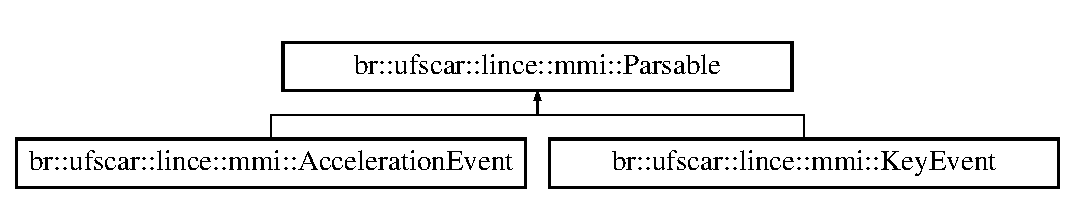
\includegraphics[height=2cm]{classbr_1_1ufscar_1_1lince_1_1mmi_1_1Parsable}
\end{center}
\end{figure}
\subsection*{Public Member Functions}
\begin{DoxyCompactItemize}
\item 
virtual \hyperlink{classbr_1_1ufscar_1_1lince_1_1mmi_1_1Parsable_ab2537805eb3b5fd91436a72edd4a3805}{$\sim$Parsable} ()
\begin{DoxyCompactList}\small\item\em Destructor. \item\end{DoxyCompactList}\item 
virtual void \hyperlink{classbr_1_1ufscar_1_1lince_1_1mmi_1_1Parsable_a6524a0a77abb3865e5d255e466b6159e}{parseXMLData} (\hyperlink{structbr_1_1ufscar_1_1lince_1_1mmi_1_1XMLData}{XMLData} $\ast$data)=0
\begin{DoxyCompactList}\small\item\em This methods realize the parse of a event represented by a XML Document. \item\end{DoxyCompactList}\item 
\hyperlink{classbr_1_1ufscar_1_1lince_1_1mmi_1_1Parsable_ade12a0d0cab87281461cca1c4bee7afd}{Parsable} ()
\begin{DoxyCompactList}\small\item\em Generic Contructor. \item\end{DoxyCompactList}\end{DoxyCompactItemize}


\subsection{Constructor \& Destructor Documentation}
\hypertarget{classbr_1_1ufscar_1_1lince_1_1mmi_1_1Parsable_ab2537805eb3b5fd91436a72edd4a3805}{
\index{br::ufscar::lince::mmi::Parsable@{br::ufscar::lince::mmi::Parsable}!$\sim$Parsable@{$\sim$Parsable}}
\index{$\sim$Parsable@{$\sim$Parsable}!br::ufscar::lince::mmi::Parsable@{br::ufscar::lince::mmi::Parsable}}
\subsubsection[{$\sim$Parsable}]{\setlength{\rightskip}{0pt plus 5cm}virtual br::ufscar::lince::mmi::Parsable::$\sim$Parsable ()\hspace{0.3cm}{\ttfamily  \mbox{[}inline, virtual\mbox{]}}}}
\label{classbr_1_1ufscar_1_1lince_1_1mmi_1_1Parsable_ab2537805eb3b5fd91436a72edd4a3805}


Destructor. 

\hypertarget{classbr_1_1ufscar_1_1lince_1_1mmi_1_1Parsable_ade12a0d0cab87281461cca1c4bee7afd}{
\index{br::ufscar::lince::mmi::Parsable@{br::ufscar::lince::mmi::Parsable}!Parsable@{Parsable}}
\index{Parsable@{Parsable}!br::ufscar::lince::mmi::Parsable@{br::ufscar::lince::mmi::Parsable}}
\subsubsection[{Parsable}]{\setlength{\rightskip}{0pt plus 5cm}br::ufscar::lince::mmi::Parsable::Parsable ()\hspace{0.3cm}{\ttfamily  \mbox{[}inline\mbox{]}}}}
\label{classbr_1_1ufscar_1_1lince_1_1mmi_1_1Parsable_ade12a0d0cab87281461cca1c4bee7afd}


Generic Contructor. 



\subsection{Member Function Documentation}
\hypertarget{classbr_1_1ufscar_1_1lince_1_1mmi_1_1Parsable_a6524a0a77abb3865e5d255e466b6159e}{
\index{br::ufscar::lince::mmi::Parsable@{br::ufscar::lince::mmi::Parsable}!parseXMLData@{parseXMLData}}
\index{parseXMLData@{parseXMLData}!br::ufscar::lince::mmi::Parsable@{br::ufscar::lince::mmi::Parsable}}
\subsubsection[{parseXMLData}]{\setlength{\rightskip}{0pt plus 5cm}virtual void br::ufscar::lince::mmi::Parsable::parseXMLData ({\bf XMLData} $\ast$ {\em data})\hspace{0.3cm}{\ttfamily  \mbox{[}pure virtual\mbox{]}}}}
\label{classbr_1_1ufscar_1_1lince_1_1mmi_1_1Parsable_a6524a0a77abb3865e5d255e466b6159e}


This methods realize the parse of a event represented by a XML Document. 


\begin{DoxyParams}{Parameters}
\item[{\em data}]A instance of \hyperlink{structbr_1_1ufscar_1_1lince_1_1mmi_1_1XMLData}{XMLData} that contains the XML Document information. \end{DoxyParams}


Implemented in \hyperlink{classbr_1_1ufscar_1_1lince_1_1mmi_1_1AccelerationEvent_a5ad5b14f13e40450e619ce08e4ba9937}{br::ufscar::lince::mmi::AccelerationEvent}.



The documentation for this class was generated from the following file:\begin{DoxyCompactItemize}
\item 
include/\hyperlink{Parsable_8h}{Parsable.h}\end{DoxyCompactItemize}

\hypertarget{classbr_1_1ufscar_1_1lince_1_1mmi_1_1socketconn_1_1ServerSocketTCP}{
\section{br::ufscar::lince::mmi::socketconn::ServerSocketTCP Class Reference}
\label{classbr_1_1ufscar_1_1lince_1_1mmi_1_1socketconn_1_1ServerSocketTCP}\index{br::ufscar::lince::mmi::socketconn::ServerSocketTCP@{br::ufscar::lince::mmi::socketconn::ServerSocketTCP}}
}


{\ttfamily \#include $<$ServerSocketTCP.h$>$}

\subsection*{Public Member Functions}
\begin{DoxyCompactItemize}
\item 
\hyperlink{classbr_1_1ufscar_1_1lince_1_1mmi_1_1socketconn_1_1ServerSocketTCP_a333eaf37843a6b92be8409057c0912d4}{ServerSocketTCP} (unsigned short port)
\item 
\hyperlink{classbr_1_1ufscar_1_1lince_1_1mmi_1_1socketconn_1_1ServerSocketTCP_a5fe635a8624663152769239eb15bb32d}{$\sim$ServerSocketTCP} ()
\item 
void \hyperlink{classbr_1_1ufscar_1_1lince_1_1mmi_1_1socketconn_1_1ServerSocketTCP_a178273f9acb926091d947e8824499c39}{bindPort} ()
\item 
void \hyperlink{classbr_1_1ufscar_1_1lince_1_1mmi_1_1socketconn_1_1ServerSocketTCP_a62f72f6e9e59f52bb2166dfe24b96404}{startListen} ()
\item 
void \hyperlink{classbr_1_1ufscar_1_1lince_1_1mmi_1_1socketconn_1_1ServerSocketTCP_a04a980f7cc35bd2c962db3959af74cbe}{startListen} (unsigned int max)
\item 
\hyperlink{classbr_1_1ufscar_1_1lince_1_1mmi_1_1socketconn_1_1SocketTCP}{SocketTCP} $\ast$ \hyperlink{classbr_1_1ufscar_1_1lince_1_1mmi_1_1socketconn_1_1ServerSocketTCP_ae47a3a55c453925c7925787487b0d80b}{acceptConnection} ()
\item 
void \hyperlink{classbr_1_1ufscar_1_1lince_1_1mmi_1_1socketconn_1_1ServerSocketTCP_a1f1be1ca0f733cf4caee8bd93b6a00eb}{releasePort} ()
\end{DoxyCompactItemize}
\subsection*{Protected Attributes}
\begin{DoxyCompactItemize}
\item 
unsigned short \hyperlink{classbr_1_1ufscar_1_1lince_1_1mmi_1_1socketconn_1_1ServerSocketTCP_ac8243d57e2882ed374c0b5c27109ec5e}{portNumber}
\end{DoxyCompactItemize}


\subsection{Constructor \& Destructor Documentation}
\hypertarget{classbr_1_1ufscar_1_1lince_1_1mmi_1_1socketconn_1_1ServerSocketTCP_a333eaf37843a6b92be8409057c0912d4}{
\index{br::ufscar::lince::mmi::socketconn::ServerSocketTCP@{br::ufscar::lince::mmi::socketconn::ServerSocketTCP}!ServerSocketTCP@{ServerSocketTCP}}
\index{ServerSocketTCP@{ServerSocketTCP}!br::ufscar::lince::mmi::socketconn::ServerSocketTCP@{br::ufscar::lince::mmi::socketconn::ServerSocketTCP}}
\subsubsection[{ServerSocketTCP}]{\setlength{\rightskip}{0pt plus 5cm}br::ufscar::lince::mmi::socketconn::ServerSocketTCP::ServerSocketTCP (unsigned short {\em port})}}
\label{classbr_1_1ufscar_1_1lince_1_1mmi_1_1socketconn_1_1ServerSocketTCP_a333eaf37843a6b92be8409057c0912d4}
\hypertarget{classbr_1_1ufscar_1_1lince_1_1mmi_1_1socketconn_1_1ServerSocketTCP_a5fe635a8624663152769239eb15bb32d}{
\index{br::ufscar::lince::mmi::socketconn::ServerSocketTCP@{br::ufscar::lince::mmi::socketconn::ServerSocketTCP}!$\sim$ServerSocketTCP@{$\sim$ServerSocketTCP}}
\index{$\sim$ServerSocketTCP@{$\sim$ServerSocketTCP}!br::ufscar::lince::mmi::socketconn::ServerSocketTCP@{br::ufscar::lince::mmi::socketconn::ServerSocketTCP}}
\subsubsection[{$\sim$ServerSocketTCP}]{\setlength{\rightskip}{0pt plus 5cm}br::ufscar::lince::mmi::socketconn::ServerSocketTCP::$\sim$ServerSocketTCP ()}}
\label{classbr_1_1ufscar_1_1lince_1_1mmi_1_1socketconn_1_1ServerSocketTCP_a5fe635a8624663152769239eb15bb32d}


\subsection{Member Function Documentation}
\hypertarget{classbr_1_1ufscar_1_1lince_1_1mmi_1_1socketconn_1_1ServerSocketTCP_ae47a3a55c453925c7925787487b0d80b}{
\index{br::ufscar::lince::mmi::socketconn::ServerSocketTCP@{br::ufscar::lince::mmi::socketconn::ServerSocketTCP}!acceptConnection@{acceptConnection}}
\index{acceptConnection@{acceptConnection}!br::ufscar::lince::mmi::socketconn::ServerSocketTCP@{br::ufscar::lince::mmi::socketconn::ServerSocketTCP}}
\subsubsection[{acceptConnection}]{\setlength{\rightskip}{0pt plus 5cm}{\bf SocketTCP}$\ast$ br::ufscar::lince::mmi::socketconn::ServerSocketTCP::acceptConnection ()}}
\label{classbr_1_1ufscar_1_1lince_1_1mmi_1_1socketconn_1_1ServerSocketTCP_ae47a3a55c453925c7925787487b0d80b}
\hypertarget{classbr_1_1ufscar_1_1lince_1_1mmi_1_1socketconn_1_1ServerSocketTCP_a178273f9acb926091d947e8824499c39}{
\index{br::ufscar::lince::mmi::socketconn::ServerSocketTCP@{br::ufscar::lince::mmi::socketconn::ServerSocketTCP}!bindPort@{bindPort}}
\index{bindPort@{bindPort}!br::ufscar::lince::mmi::socketconn::ServerSocketTCP@{br::ufscar::lince::mmi::socketconn::ServerSocketTCP}}
\subsubsection[{bindPort}]{\setlength{\rightskip}{0pt plus 5cm}void br::ufscar::lince::mmi::socketconn::ServerSocketTCP::bindPort ()}}
\label{classbr_1_1ufscar_1_1lince_1_1mmi_1_1socketconn_1_1ServerSocketTCP_a178273f9acb926091d947e8824499c39}
\hypertarget{classbr_1_1ufscar_1_1lince_1_1mmi_1_1socketconn_1_1ServerSocketTCP_a1f1be1ca0f733cf4caee8bd93b6a00eb}{
\index{br::ufscar::lince::mmi::socketconn::ServerSocketTCP@{br::ufscar::lince::mmi::socketconn::ServerSocketTCP}!releasePort@{releasePort}}
\index{releasePort@{releasePort}!br::ufscar::lince::mmi::socketconn::ServerSocketTCP@{br::ufscar::lince::mmi::socketconn::ServerSocketTCP}}
\subsubsection[{releasePort}]{\setlength{\rightskip}{0pt plus 5cm}void br::ufscar::lince::mmi::socketconn::ServerSocketTCP::releasePort ()}}
\label{classbr_1_1ufscar_1_1lince_1_1mmi_1_1socketconn_1_1ServerSocketTCP_a1f1be1ca0f733cf4caee8bd93b6a00eb}
\hypertarget{classbr_1_1ufscar_1_1lince_1_1mmi_1_1socketconn_1_1ServerSocketTCP_a04a980f7cc35bd2c962db3959af74cbe}{
\index{br::ufscar::lince::mmi::socketconn::ServerSocketTCP@{br::ufscar::lince::mmi::socketconn::ServerSocketTCP}!startListen@{startListen}}
\index{startListen@{startListen}!br::ufscar::lince::mmi::socketconn::ServerSocketTCP@{br::ufscar::lince::mmi::socketconn::ServerSocketTCP}}
\subsubsection[{startListen}]{\setlength{\rightskip}{0pt plus 5cm}void br::ufscar::lince::mmi::socketconn::ServerSocketTCP::startListen (unsigned int {\em max})}}
\label{classbr_1_1ufscar_1_1lince_1_1mmi_1_1socketconn_1_1ServerSocketTCP_a04a980f7cc35bd2c962db3959af74cbe}
\hypertarget{classbr_1_1ufscar_1_1lince_1_1mmi_1_1socketconn_1_1ServerSocketTCP_a62f72f6e9e59f52bb2166dfe24b96404}{
\index{br::ufscar::lince::mmi::socketconn::ServerSocketTCP@{br::ufscar::lince::mmi::socketconn::ServerSocketTCP}!startListen@{startListen}}
\index{startListen@{startListen}!br::ufscar::lince::mmi::socketconn::ServerSocketTCP@{br::ufscar::lince::mmi::socketconn::ServerSocketTCP}}
\subsubsection[{startListen}]{\setlength{\rightskip}{0pt plus 5cm}void br::ufscar::lince::mmi::socketconn::ServerSocketTCP::startListen ()}}
\label{classbr_1_1ufscar_1_1lince_1_1mmi_1_1socketconn_1_1ServerSocketTCP_a62f72f6e9e59f52bb2166dfe24b96404}


\subsection{Field Documentation}
\hypertarget{classbr_1_1ufscar_1_1lince_1_1mmi_1_1socketconn_1_1ServerSocketTCP_ac8243d57e2882ed374c0b5c27109ec5e}{
\index{br::ufscar::lince::mmi::socketconn::ServerSocketTCP@{br::ufscar::lince::mmi::socketconn::ServerSocketTCP}!portNumber@{portNumber}}
\index{portNumber@{portNumber}!br::ufscar::lince::mmi::socketconn::ServerSocketTCP@{br::ufscar::lince::mmi::socketconn::ServerSocketTCP}}
\subsubsection[{portNumber}]{\setlength{\rightskip}{0pt plus 5cm}unsigned short {\bf br::ufscar::lince::mmi::socketconn::ServerSocketTCP::portNumber}\hspace{0.3cm}{\ttfamily  \mbox{[}protected\mbox{]}}}}
\label{classbr_1_1ufscar_1_1lince_1_1mmi_1_1socketconn_1_1ServerSocketTCP_ac8243d57e2882ed374c0b5c27109ec5e}


The documentation for this class was generated from the following file:\begin{DoxyCompactItemize}
\item 
include/socketconn/\hyperlink{ServerSocketTCP_8h}{ServerSocketTCP.h}\end{DoxyCompactItemize}

\hypertarget{classbr_1_1ufscar_1_1lince_1_1mmi_1_1socketconn_1_1SocketTCP}{
\section{br::ufscar::lince::mmi::socketconn::SocketTCP Class Reference}
\label{classbr_1_1ufscar_1_1lince_1_1mmi_1_1socketconn_1_1SocketTCP}\index{br::ufscar::lince::mmi::socketconn::SocketTCP@{br::ufscar::lince::mmi::socketconn::SocketTCP}}
}


{\ttfamily \#include $<$SocketTCP.h$>$}

\subsection*{Public Member Functions}
\begin{DoxyCompactItemize}
\item 
\hyperlink{classbr_1_1ufscar_1_1lince_1_1mmi_1_1socketconn_1_1SocketTCP_a98f391c314ca7210a8cdcfc666307540}{SocketTCP} (string ip, unsigned short port)
\item 
void \hyperlink{classbr_1_1ufscar_1_1lince_1_1mmi_1_1socketconn_1_1SocketTCP_a02b9574bbf468265f8781bd0ed2ea913}{connectSocket} ()
\item 
\hyperlink{classbr_1_1ufscar_1_1lince_1_1mmi_1_1socketconn_1_1DataPayload}{DataPayload} $\ast$ \hyperlink{classbr_1_1ufscar_1_1lince_1_1mmi_1_1socketconn_1_1SocketTCP_a2b577c784c4b34867851108230c5dedd}{reciveData} ()
\item 
int \hyperlink{classbr_1_1ufscar_1_1lince_1_1mmi_1_1socketconn_1_1SocketTCP_ae677b051d5e7a83bd0e3b7b947c5256b}{sendData} (\hyperlink{classbr_1_1ufscar_1_1lince_1_1mmi_1_1socketconn_1_1DataPayload}{DataPayload} $\ast$data)
\item 
void \hyperlink{classbr_1_1ufscar_1_1lince_1_1mmi_1_1socketconn_1_1SocketTCP_a109ecde95cef2c487193e5c256fef695}{closeConnection} ()
\item 
string \hyperlink{classbr_1_1ufscar_1_1lince_1_1mmi_1_1socketconn_1_1SocketTCP_a414912f61f221d793a2d9db8e919e2d5}{getIPAddress} ()
\item 
unsigned short \hyperlink{classbr_1_1ufscar_1_1lince_1_1mmi_1_1socketconn_1_1SocketTCP_a242631145b3bab7c7d6c08c5b76eb39a}{getPortNumber} ()
\end{DoxyCompactItemize}
\subsection*{Protected Member Functions}
\begin{DoxyCompactItemize}
\item 
\hyperlink{classbr_1_1ufscar_1_1lince_1_1mmi_1_1socketconn_1_1SocketTCP_a9df5b18236cbacc41a53d9d4fc320a8a}{SocketTCP} (int clientSocket, sockaddr\_\-in clientAddres)
\end{DoxyCompactItemize}
\subsection*{Friends}
\begin{DoxyCompactItemize}
\item 
class \hyperlink{classbr_1_1ufscar_1_1lince_1_1mmi_1_1socketconn_1_1SocketTCP_a1fb2b529851e5c95e720a67fbc1aaaa1}{ServerSocketTCP}
\end{DoxyCompactItemize}


\subsection{Constructor \& Destructor Documentation}
\hypertarget{classbr_1_1ufscar_1_1lince_1_1mmi_1_1socketconn_1_1SocketTCP_a98f391c314ca7210a8cdcfc666307540}{
\index{br::ufscar::lince::mmi::socketconn::SocketTCP@{br::ufscar::lince::mmi::socketconn::SocketTCP}!SocketTCP@{SocketTCP}}
\index{SocketTCP@{SocketTCP}!br::ufscar::lince::mmi::socketconn::SocketTCP@{br::ufscar::lince::mmi::socketconn::SocketTCP}}
\subsubsection[{SocketTCP}]{\setlength{\rightskip}{0pt plus 5cm}br::ufscar::lince::mmi::socketconn::SocketTCP::SocketTCP (string {\em ip}, \/  unsigned short {\em port})}}
\label{classbr_1_1ufscar_1_1lince_1_1mmi_1_1socketconn_1_1SocketTCP_a98f391c314ca7210a8cdcfc666307540}
\hypertarget{classbr_1_1ufscar_1_1lince_1_1mmi_1_1socketconn_1_1SocketTCP_a9df5b18236cbacc41a53d9d4fc320a8a}{
\index{br::ufscar::lince::mmi::socketconn::SocketTCP@{br::ufscar::lince::mmi::socketconn::SocketTCP}!SocketTCP@{SocketTCP}}
\index{SocketTCP@{SocketTCP}!br::ufscar::lince::mmi::socketconn::SocketTCP@{br::ufscar::lince::mmi::socketconn::SocketTCP}}
\subsubsection[{SocketTCP}]{\setlength{\rightskip}{0pt plus 5cm}br::ufscar::lince::mmi::socketconn::SocketTCP::SocketTCP (int {\em clientSocket}, \/  sockaddr\_\-in {\em clientAddres})\hspace{0.3cm}{\ttfamily  \mbox{[}protected\mbox{]}}}}
\label{classbr_1_1ufscar_1_1lince_1_1mmi_1_1socketconn_1_1SocketTCP_a9df5b18236cbacc41a53d9d4fc320a8a}


\subsection{Member Function Documentation}
\hypertarget{classbr_1_1ufscar_1_1lince_1_1mmi_1_1socketconn_1_1SocketTCP_a109ecde95cef2c487193e5c256fef695}{
\index{br::ufscar::lince::mmi::socketconn::SocketTCP@{br::ufscar::lince::mmi::socketconn::SocketTCP}!closeConnection@{closeConnection}}
\index{closeConnection@{closeConnection}!br::ufscar::lince::mmi::socketconn::SocketTCP@{br::ufscar::lince::mmi::socketconn::SocketTCP}}
\subsubsection[{closeConnection}]{\setlength{\rightskip}{0pt plus 5cm}void br::ufscar::lince::mmi::socketconn::SocketTCP::closeConnection ()}}
\label{classbr_1_1ufscar_1_1lince_1_1mmi_1_1socketconn_1_1SocketTCP_a109ecde95cef2c487193e5c256fef695}
\hypertarget{classbr_1_1ufscar_1_1lince_1_1mmi_1_1socketconn_1_1SocketTCP_a02b9574bbf468265f8781bd0ed2ea913}{
\index{br::ufscar::lince::mmi::socketconn::SocketTCP@{br::ufscar::lince::mmi::socketconn::SocketTCP}!connectSocket@{connectSocket}}
\index{connectSocket@{connectSocket}!br::ufscar::lince::mmi::socketconn::SocketTCP@{br::ufscar::lince::mmi::socketconn::SocketTCP}}
\subsubsection[{connectSocket}]{\setlength{\rightskip}{0pt plus 5cm}void br::ufscar::lince::mmi::socketconn::SocketTCP::connectSocket ()}}
\label{classbr_1_1ufscar_1_1lince_1_1mmi_1_1socketconn_1_1SocketTCP_a02b9574bbf468265f8781bd0ed2ea913}
\hypertarget{classbr_1_1ufscar_1_1lince_1_1mmi_1_1socketconn_1_1SocketTCP_a414912f61f221d793a2d9db8e919e2d5}{
\index{br::ufscar::lince::mmi::socketconn::SocketTCP@{br::ufscar::lince::mmi::socketconn::SocketTCP}!getIPAddress@{getIPAddress}}
\index{getIPAddress@{getIPAddress}!br::ufscar::lince::mmi::socketconn::SocketTCP@{br::ufscar::lince::mmi::socketconn::SocketTCP}}
\subsubsection[{getIPAddress}]{\setlength{\rightskip}{0pt plus 5cm}string br::ufscar::lince::mmi::socketconn::SocketTCP::getIPAddress ()}}
\label{classbr_1_1ufscar_1_1lince_1_1mmi_1_1socketconn_1_1SocketTCP_a414912f61f221d793a2d9db8e919e2d5}
\hypertarget{classbr_1_1ufscar_1_1lince_1_1mmi_1_1socketconn_1_1SocketTCP_a242631145b3bab7c7d6c08c5b76eb39a}{
\index{br::ufscar::lince::mmi::socketconn::SocketTCP@{br::ufscar::lince::mmi::socketconn::SocketTCP}!getPortNumber@{getPortNumber}}
\index{getPortNumber@{getPortNumber}!br::ufscar::lince::mmi::socketconn::SocketTCP@{br::ufscar::lince::mmi::socketconn::SocketTCP}}
\subsubsection[{getPortNumber}]{\setlength{\rightskip}{0pt plus 5cm}unsigned short br::ufscar::lince::mmi::socketconn::SocketTCP::getPortNumber ()}}
\label{classbr_1_1ufscar_1_1lince_1_1mmi_1_1socketconn_1_1SocketTCP_a242631145b3bab7c7d6c08c5b76eb39a}
\hypertarget{classbr_1_1ufscar_1_1lince_1_1mmi_1_1socketconn_1_1SocketTCP_a2b577c784c4b34867851108230c5dedd}{
\index{br::ufscar::lince::mmi::socketconn::SocketTCP@{br::ufscar::lince::mmi::socketconn::SocketTCP}!reciveData@{reciveData}}
\index{reciveData@{reciveData}!br::ufscar::lince::mmi::socketconn::SocketTCP@{br::ufscar::lince::mmi::socketconn::SocketTCP}}
\subsubsection[{reciveData}]{\setlength{\rightskip}{0pt plus 5cm}{\bf DataPayload}$\ast$ br::ufscar::lince::mmi::socketconn::SocketTCP::reciveData ()}}
\label{classbr_1_1ufscar_1_1lince_1_1mmi_1_1socketconn_1_1SocketTCP_a2b577c784c4b34867851108230c5dedd}
\hypertarget{classbr_1_1ufscar_1_1lince_1_1mmi_1_1socketconn_1_1SocketTCP_ae677b051d5e7a83bd0e3b7b947c5256b}{
\index{br::ufscar::lince::mmi::socketconn::SocketTCP@{br::ufscar::lince::mmi::socketconn::SocketTCP}!sendData@{sendData}}
\index{sendData@{sendData}!br::ufscar::lince::mmi::socketconn::SocketTCP@{br::ufscar::lince::mmi::socketconn::SocketTCP}}
\subsubsection[{sendData}]{\setlength{\rightskip}{0pt plus 5cm}int br::ufscar::lince::mmi::socketconn::SocketTCP::sendData ({\bf DataPayload} $\ast$ {\em data})}}
\label{classbr_1_1ufscar_1_1lince_1_1mmi_1_1socketconn_1_1SocketTCP_ae677b051d5e7a83bd0e3b7b947c5256b}


\subsection{Friends And Related Function Documentation}
\hypertarget{classbr_1_1ufscar_1_1lince_1_1mmi_1_1socketconn_1_1SocketTCP_a1fb2b529851e5c95e720a67fbc1aaaa1}{
\index{br::ufscar::lince::mmi::socketconn::SocketTCP@{br::ufscar::lince::mmi::socketconn::SocketTCP}!ServerSocketTCP@{ServerSocketTCP}}
\index{ServerSocketTCP@{ServerSocketTCP}!br::ufscar::lince::mmi::socketconn::SocketTCP@{br::ufscar::lince::mmi::socketconn::SocketTCP}}
\subsubsection[{ServerSocketTCP}]{\setlength{\rightskip}{0pt plus 5cm}friend class {\bf ServerSocketTCP}\hspace{0.3cm}{\ttfamily  \mbox{[}friend\mbox{]}}}}
\label{classbr_1_1ufscar_1_1lince_1_1mmi_1_1socketconn_1_1SocketTCP_a1fb2b529851e5c95e720a67fbc1aaaa1}


The documentation for this class was generated from the following file:\begin{DoxyCompactItemize}
\item 
include/socketconn/\hyperlink{SocketTCP_8h}{SocketTCP.h}\end{DoxyCompactItemize}

\hypertarget{classbr_1_1ufscar_1_1lince_1_1mmi_1_1wii_1_1StateCircularBuffer}{
\section{br::ufscar::lince::mmi::wii::StateCircularBuffer Class Reference}
\label{classbr_1_1ufscar_1_1lince_1_1mmi_1_1wii_1_1StateCircularBuffer}\index{br::ufscar::lince::mmi::wii::StateCircularBuffer@{br::ufscar::lince::mmi::wii::StateCircularBuffer}}
}


{\ttfamily \#include $<$StateCircularBuffer.h$>$}

\subsection*{Public Member Functions}
\begin{DoxyCompactItemize}
\item 
\hyperlink{classbr_1_1ufscar_1_1lince_1_1mmi_1_1wii_1_1StateCircularBuffer_a33314840ca4d71cf5d391e292ca9bc3e}{StateCircularBuffer} (int size=10)
\item 
virtual \hyperlink{classbr_1_1ufscar_1_1lince_1_1mmi_1_1wii_1_1StateCircularBuffer_a9152c8d7c2692a46c07f7e57b5683d72}{$\sim$StateCircularBuffer} ()
\item 
int \hyperlink{classbr_1_1ufscar_1_1lince_1_1mmi_1_1wii_1_1StateCircularBuffer_a8a445af0ab01386fb42cfb2523472ddf}{getCurrentSize} ()
\item 
int \hyperlink{classbr_1_1ufscar_1_1lince_1_1mmi_1_1wii_1_1StateCircularBuffer_a3b762c90ccda72c94da995d8c6d5cac6}{getMaxSize} ()
\item 
void \hyperlink{classbr_1_1ufscar_1_1lince_1_1mmi_1_1wii_1_1StateCircularBuffer_a8d4ed07d00ae3cd16e56c8dbe42c0334}{insert} (\hyperlink{classbr_1_1ufscar_1_1lince_1_1mmi_1_1wii_1_1WiiState}{WiiState} $\ast$state)
\item 
\hyperlink{classbr_1_1ufscar_1_1lince_1_1mmi_1_1wii_1_1WiiState}{WiiState} $\ast$ \hyperlink{classbr_1_1ufscar_1_1lince_1_1mmi_1_1wii_1_1StateCircularBuffer_a41bb3dd2846d5038b69fce4d65ba907a}{remove} ()
\item 
\hyperlink{classbr_1_1ufscar_1_1lince_1_1mmi_1_1wii_1_1WiiState}{WiiState} $\ast$ \hyperlink{classbr_1_1ufscar_1_1lince_1_1mmi_1_1wii_1_1StateCircularBuffer_a369047a3b4e1d99e0a997b8ab7e1a476}{take} ()
\item 
bool \hyperlink{classbr_1_1ufscar_1_1lince_1_1mmi_1_1wii_1_1StateCircularBuffer_a4beeb8af8698021f10d719b77d5c4427}{isEmpty} ()
\item 
void \hyperlink{classbr_1_1ufscar_1_1lince_1_1mmi_1_1wii_1_1StateCircularBuffer_ad5e7282be7550aaa267eea85c4f569a2}{showAllStates} ()
\item 
\hyperlink{classbr_1_1ufscar_1_1lince_1_1mmi_1_1wii_1_1WiiState}{WiiState} $\ast$ \hyperlink{classbr_1_1ufscar_1_1lince_1_1mmi_1_1wii_1_1StateCircularBuffer_aaf271d9993fd69eaff64a6b31bb6173f}{getBegin} ()
\item 
\hyperlink{classbr_1_1ufscar_1_1lince_1_1mmi_1_1wii_1_1WiiState}{WiiState} $\ast$ \hyperlink{classbr_1_1ufscar_1_1lince_1_1mmi_1_1wii_1_1StateCircularBuffer_ae29b35bd8e817d3dfb8c10b51c920e1a}{getNext} ()
\end{DoxyCompactItemize}


\subsection{Constructor \& Destructor Documentation}
\hypertarget{classbr_1_1ufscar_1_1lince_1_1mmi_1_1wii_1_1StateCircularBuffer_a33314840ca4d71cf5d391e292ca9bc3e}{
\index{br::ufscar::lince::mmi::wii::StateCircularBuffer@{br::ufscar::lince::mmi::wii::StateCircularBuffer}!StateCircularBuffer@{StateCircularBuffer}}
\index{StateCircularBuffer@{StateCircularBuffer}!br::ufscar::lince::mmi::wii::StateCircularBuffer@{br::ufscar::lince::mmi::wii::StateCircularBuffer}}
\subsubsection[{StateCircularBuffer}]{\setlength{\rightskip}{0pt plus 5cm}br::ufscar::lince::mmi::wii::StateCircularBuffer::StateCircularBuffer (int {\em size} = {\ttfamily 10})}}
\label{classbr_1_1ufscar_1_1lince_1_1mmi_1_1wii_1_1StateCircularBuffer_a33314840ca4d71cf5d391e292ca9bc3e}
\hypertarget{classbr_1_1ufscar_1_1lince_1_1mmi_1_1wii_1_1StateCircularBuffer_a9152c8d7c2692a46c07f7e57b5683d72}{
\index{br::ufscar::lince::mmi::wii::StateCircularBuffer@{br::ufscar::lince::mmi::wii::StateCircularBuffer}!$\sim$StateCircularBuffer@{$\sim$StateCircularBuffer}}
\index{$\sim$StateCircularBuffer@{$\sim$StateCircularBuffer}!br::ufscar::lince::mmi::wii::StateCircularBuffer@{br::ufscar::lince::mmi::wii::StateCircularBuffer}}
\subsubsection[{$\sim$StateCircularBuffer}]{\setlength{\rightskip}{0pt plus 5cm}virtual br::ufscar::lince::mmi::wii::StateCircularBuffer::$\sim$StateCircularBuffer ()\hspace{0.3cm}{\ttfamily  \mbox{[}virtual\mbox{]}}}}
\label{classbr_1_1ufscar_1_1lince_1_1mmi_1_1wii_1_1StateCircularBuffer_a9152c8d7c2692a46c07f7e57b5683d72}


\subsection{Member Function Documentation}
\hypertarget{classbr_1_1ufscar_1_1lince_1_1mmi_1_1wii_1_1StateCircularBuffer_aaf271d9993fd69eaff64a6b31bb6173f}{
\index{br::ufscar::lince::mmi::wii::StateCircularBuffer@{br::ufscar::lince::mmi::wii::StateCircularBuffer}!getBegin@{getBegin}}
\index{getBegin@{getBegin}!br::ufscar::lince::mmi::wii::StateCircularBuffer@{br::ufscar::lince::mmi::wii::StateCircularBuffer}}
\subsubsection[{getBegin}]{\setlength{\rightskip}{0pt plus 5cm}{\bf WiiState}$\ast$ br::ufscar::lince::mmi::wii::StateCircularBuffer::getBegin ()}}
\label{classbr_1_1ufscar_1_1lince_1_1mmi_1_1wii_1_1StateCircularBuffer_aaf271d9993fd69eaff64a6b31bb6173f}
\hypertarget{classbr_1_1ufscar_1_1lince_1_1mmi_1_1wii_1_1StateCircularBuffer_a8a445af0ab01386fb42cfb2523472ddf}{
\index{br::ufscar::lince::mmi::wii::StateCircularBuffer@{br::ufscar::lince::mmi::wii::StateCircularBuffer}!getCurrentSize@{getCurrentSize}}
\index{getCurrentSize@{getCurrentSize}!br::ufscar::lince::mmi::wii::StateCircularBuffer@{br::ufscar::lince::mmi::wii::StateCircularBuffer}}
\subsubsection[{getCurrentSize}]{\setlength{\rightskip}{0pt plus 5cm}int br::ufscar::lince::mmi::wii::StateCircularBuffer::getCurrentSize ()}}
\label{classbr_1_1ufscar_1_1lince_1_1mmi_1_1wii_1_1StateCircularBuffer_a8a445af0ab01386fb42cfb2523472ddf}
\hypertarget{classbr_1_1ufscar_1_1lince_1_1mmi_1_1wii_1_1StateCircularBuffer_a3b762c90ccda72c94da995d8c6d5cac6}{
\index{br::ufscar::lince::mmi::wii::StateCircularBuffer@{br::ufscar::lince::mmi::wii::StateCircularBuffer}!getMaxSize@{getMaxSize}}
\index{getMaxSize@{getMaxSize}!br::ufscar::lince::mmi::wii::StateCircularBuffer@{br::ufscar::lince::mmi::wii::StateCircularBuffer}}
\subsubsection[{getMaxSize}]{\setlength{\rightskip}{0pt plus 5cm}int br::ufscar::lince::mmi::wii::StateCircularBuffer::getMaxSize ()}}
\label{classbr_1_1ufscar_1_1lince_1_1mmi_1_1wii_1_1StateCircularBuffer_a3b762c90ccda72c94da995d8c6d5cac6}
\hypertarget{classbr_1_1ufscar_1_1lince_1_1mmi_1_1wii_1_1StateCircularBuffer_ae29b35bd8e817d3dfb8c10b51c920e1a}{
\index{br::ufscar::lince::mmi::wii::StateCircularBuffer@{br::ufscar::lince::mmi::wii::StateCircularBuffer}!getNext@{getNext}}
\index{getNext@{getNext}!br::ufscar::lince::mmi::wii::StateCircularBuffer@{br::ufscar::lince::mmi::wii::StateCircularBuffer}}
\subsubsection[{getNext}]{\setlength{\rightskip}{0pt plus 5cm}{\bf WiiState}$\ast$ br::ufscar::lince::mmi::wii::StateCircularBuffer::getNext ()}}
\label{classbr_1_1ufscar_1_1lince_1_1mmi_1_1wii_1_1StateCircularBuffer_ae29b35bd8e817d3dfb8c10b51c920e1a}
\hypertarget{classbr_1_1ufscar_1_1lince_1_1mmi_1_1wii_1_1StateCircularBuffer_a8d4ed07d00ae3cd16e56c8dbe42c0334}{
\index{br::ufscar::lince::mmi::wii::StateCircularBuffer@{br::ufscar::lince::mmi::wii::StateCircularBuffer}!insert@{insert}}
\index{insert@{insert}!br::ufscar::lince::mmi::wii::StateCircularBuffer@{br::ufscar::lince::mmi::wii::StateCircularBuffer}}
\subsubsection[{insert}]{\setlength{\rightskip}{0pt plus 5cm}void br::ufscar::lince::mmi::wii::StateCircularBuffer::insert ({\bf WiiState} $\ast$ {\em state})}}
\label{classbr_1_1ufscar_1_1lince_1_1mmi_1_1wii_1_1StateCircularBuffer_a8d4ed07d00ae3cd16e56c8dbe42c0334}
\hypertarget{classbr_1_1ufscar_1_1lince_1_1mmi_1_1wii_1_1StateCircularBuffer_a4beeb8af8698021f10d719b77d5c4427}{
\index{br::ufscar::lince::mmi::wii::StateCircularBuffer@{br::ufscar::lince::mmi::wii::StateCircularBuffer}!isEmpty@{isEmpty}}
\index{isEmpty@{isEmpty}!br::ufscar::lince::mmi::wii::StateCircularBuffer@{br::ufscar::lince::mmi::wii::StateCircularBuffer}}
\subsubsection[{isEmpty}]{\setlength{\rightskip}{0pt plus 5cm}bool br::ufscar::lince::mmi::wii::StateCircularBuffer::isEmpty ()}}
\label{classbr_1_1ufscar_1_1lince_1_1mmi_1_1wii_1_1StateCircularBuffer_a4beeb8af8698021f10d719b77d5c4427}
\hypertarget{classbr_1_1ufscar_1_1lince_1_1mmi_1_1wii_1_1StateCircularBuffer_a41bb3dd2846d5038b69fce4d65ba907a}{
\index{br::ufscar::lince::mmi::wii::StateCircularBuffer@{br::ufscar::lince::mmi::wii::StateCircularBuffer}!remove@{remove}}
\index{remove@{remove}!br::ufscar::lince::mmi::wii::StateCircularBuffer@{br::ufscar::lince::mmi::wii::StateCircularBuffer}}
\subsubsection[{remove}]{\setlength{\rightskip}{0pt plus 5cm}{\bf WiiState}$\ast$ br::ufscar::lince::mmi::wii::StateCircularBuffer::remove ()}}
\label{classbr_1_1ufscar_1_1lince_1_1mmi_1_1wii_1_1StateCircularBuffer_a41bb3dd2846d5038b69fce4d65ba907a}
\hypertarget{classbr_1_1ufscar_1_1lince_1_1mmi_1_1wii_1_1StateCircularBuffer_ad5e7282be7550aaa267eea85c4f569a2}{
\index{br::ufscar::lince::mmi::wii::StateCircularBuffer@{br::ufscar::lince::mmi::wii::StateCircularBuffer}!showAllStates@{showAllStates}}
\index{showAllStates@{showAllStates}!br::ufscar::lince::mmi::wii::StateCircularBuffer@{br::ufscar::lince::mmi::wii::StateCircularBuffer}}
\subsubsection[{showAllStates}]{\setlength{\rightskip}{0pt plus 5cm}void br::ufscar::lince::mmi::wii::StateCircularBuffer::showAllStates ()}}
\label{classbr_1_1ufscar_1_1lince_1_1mmi_1_1wii_1_1StateCircularBuffer_ad5e7282be7550aaa267eea85c4f569a2}
\hypertarget{classbr_1_1ufscar_1_1lince_1_1mmi_1_1wii_1_1StateCircularBuffer_a369047a3b4e1d99e0a997b8ab7e1a476}{
\index{br::ufscar::lince::mmi::wii::StateCircularBuffer@{br::ufscar::lince::mmi::wii::StateCircularBuffer}!take@{take}}
\index{take@{take}!br::ufscar::lince::mmi::wii::StateCircularBuffer@{br::ufscar::lince::mmi::wii::StateCircularBuffer}}
\subsubsection[{take}]{\setlength{\rightskip}{0pt plus 5cm}{\bf WiiState}$\ast$ br::ufscar::lince::mmi::wii::StateCircularBuffer::take ()}}
\label{classbr_1_1ufscar_1_1lince_1_1mmi_1_1wii_1_1StateCircularBuffer_a369047a3b4e1d99e0a997b8ab7e1a476}


The documentation for this class was generated from the following file:\begin{DoxyCompactItemize}
\item 
include/wii/\hyperlink{StateCircularBuffer_8h}{StateCircularBuffer.h}\end{DoxyCompactItemize}

\hypertarget{structbr_1_1ufscar_1_1lince_1_1mmi_1_1ink_1_1structBoundingBox}{
\section{br::ufscar::lince::mmi::ink::structBoundingBox Struct Reference}
\label{structbr_1_1ufscar_1_1lince_1_1mmi_1_1ink_1_1structBoundingBox}\index{br::ufscar::lince::mmi::ink::structBoundingBox@{br::ufscar::lince::mmi::ink::structBoundingBox}}
}


Desc -\/ structure to define the BoundingBox of the trace data and hence helps in normalizing trace co-\/ordinate data to fit in the rendering area co-\/ordinate.  




{\ttfamily \#include $<$Utility.h$>$}

\subsection*{Data Fields}
\begin{DoxyCompactItemize}
\item 
long \hyperlink{structbr_1_1ufscar_1_1lince_1_1mmi_1_1ink_1_1structBoundingBox_a0ee9f3312a600d5e18864edff981aff2}{minX}
\begin{DoxyCompactList}\small\item\em Limite inferior horizontal. \item\end{DoxyCompactList}\item 
long \hyperlink{structbr_1_1ufscar_1_1lince_1_1mmi_1_1ink_1_1structBoundingBox_a45f3a13363b8016024e8ccc5c39eae70}{minY}
\begin{DoxyCompactList}\small\item\em Limite superior vertical. \item\end{DoxyCompactList}\item 
long \hyperlink{structbr_1_1ufscar_1_1lince_1_1mmi_1_1ink_1_1structBoundingBox_a65a9d52b3d44834668ec591c9593af24}{maxX}
\begin{DoxyCompactList}\small\item\em Limite superior horizontal. \item\end{DoxyCompactList}\item 
long \hyperlink{structbr_1_1ufscar_1_1lince_1_1mmi_1_1ink_1_1structBoundingBox_ae63289fbb7f7a17ac4e44837edf362d0}{maxY}
\begin{DoxyCompactList}\small\item\em Limite inferior vertical. \item\end{DoxyCompactList}\end{DoxyCompactItemize}


\subsection{Detailed Description}
Desc -\/ structure to define the BoundingBox of the trace data and hence helps in normalizing trace co-\/ordinate data to fit in the rendering area co-\/ordinate. 

\subsection{Field Documentation}
\hypertarget{structbr_1_1ufscar_1_1lince_1_1mmi_1_1ink_1_1structBoundingBox_a65a9d52b3d44834668ec591c9593af24}{
\index{br::ufscar::lince::mmi::ink::structBoundingBox@{br::ufscar::lince::mmi::ink::structBoundingBox}!maxX@{maxX}}
\index{maxX@{maxX}!br::ufscar::lince::mmi::ink::structBoundingBox@{br::ufscar::lince::mmi::ink::structBoundingBox}}
\subsubsection[{maxX}]{\setlength{\rightskip}{0pt plus 5cm}long {\bf br::ufscar::lince::mmi::ink::structBoundingBox::maxX}}}
\label{structbr_1_1ufscar_1_1lince_1_1mmi_1_1ink_1_1structBoundingBox_a65a9d52b3d44834668ec591c9593af24}


Limite superior horizontal. 

\hypertarget{structbr_1_1ufscar_1_1lince_1_1mmi_1_1ink_1_1structBoundingBox_ae63289fbb7f7a17ac4e44837edf362d0}{
\index{br::ufscar::lince::mmi::ink::structBoundingBox@{br::ufscar::lince::mmi::ink::structBoundingBox}!maxY@{maxY}}
\index{maxY@{maxY}!br::ufscar::lince::mmi::ink::structBoundingBox@{br::ufscar::lince::mmi::ink::structBoundingBox}}
\subsubsection[{maxY}]{\setlength{\rightskip}{0pt plus 5cm}long {\bf br::ufscar::lince::mmi::ink::structBoundingBox::maxY}}}
\label{structbr_1_1ufscar_1_1lince_1_1mmi_1_1ink_1_1structBoundingBox_ae63289fbb7f7a17ac4e44837edf362d0}


Limite inferior vertical. 

\hypertarget{structbr_1_1ufscar_1_1lince_1_1mmi_1_1ink_1_1structBoundingBox_a0ee9f3312a600d5e18864edff981aff2}{
\index{br::ufscar::lince::mmi::ink::structBoundingBox@{br::ufscar::lince::mmi::ink::structBoundingBox}!minX@{minX}}
\index{minX@{minX}!br::ufscar::lince::mmi::ink::structBoundingBox@{br::ufscar::lince::mmi::ink::structBoundingBox}}
\subsubsection[{minX}]{\setlength{\rightskip}{0pt plus 5cm}long {\bf br::ufscar::lince::mmi::ink::structBoundingBox::minX}}}
\label{structbr_1_1ufscar_1_1lince_1_1mmi_1_1ink_1_1structBoundingBox_a0ee9f3312a600d5e18864edff981aff2}


Limite inferior horizontal. 

\hypertarget{structbr_1_1ufscar_1_1lince_1_1mmi_1_1ink_1_1structBoundingBox_a45f3a13363b8016024e8ccc5c39eae70}{
\index{br::ufscar::lince::mmi::ink::structBoundingBox@{br::ufscar::lince::mmi::ink::structBoundingBox}!minY@{minY}}
\index{minY@{minY}!br::ufscar::lince::mmi::ink::structBoundingBox@{br::ufscar::lince::mmi::ink::structBoundingBox}}
\subsubsection[{minY}]{\setlength{\rightskip}{0pt plus 5cm}long {\bf br::ufscar::lince::mmi::ink::structBoundingBox::minY}}}
\label{structbr_1_1ufscar_1_1lince_1_1mmi_1_1ink_1_1structBoundingBox_a45f3a13363b8016024e8ccc5c39eae70}


Limite superior vertical. 



The documentation for this struct was generated from the following file:\begin{DoxyCompactItemize}
\item 
include/ink/\hyperlink{Utility_8h}{Utility.h}\end{DoxyCompactItemize}

\hypertarget{classbr_1_1ufscar_1_1lince_1_1mmi_1_1socketconn_1_1TCPCommServer}{
\section{br::ufscar::lince::mmi::socketconn::TCPCommServer Class Reference}
\label{classbr_1_1ufscar_1_1lince_1_1mmi_1_1socketconn_1_1TCPCommServer}\index{br::ufscar::lince::mmi::socketconn::TCPCommServer@{br::ufscar::lince::mmi::socketconn::TCPCommServer}}
}


{\ttfamily \#include $<$TCPCommServer.h$>$}

\subsection*{Public Member Functions}
\begin{DoxyCompactItemize}
\item 
\hyperlink{classbr_1_1ufscar_1_1lince_1_1mmi_1_1socketconn_1_1TCPCommServer_a3f53b0b1078c2b1c3bf6975eddcc2bd2}{TCPCommServer} (int portnumber=DEFAULT\_\-PORT)
\item 
\hyperlink{classbr_1_1ufscar_1_1lince_1_1mmi_1_1socketconn_1_1TCPCommServer_a528689c5a4c14f578cfdc659a03f4c99}{$\sim$TCPCommServer} ()
\item 
void \hyperlink{classbr_1_1ufscar_1_1lince_1_1mmi_1_1socketconn_1_1TCPCommServer_ad34949969d9e206c46e71d5f9c86c44d}{release} ()
\end{DoxyCompactItemize}


\subsection{Constructor \& Destructor Documentation}
\hypertarget{classbr_1_1ufscar_1_1lince_1_1mmi_1_1socketconn_1_1TCPCommServer_a3f53b0b1078c2b1c3bf6975eddcc2bd2}{
\index{br::ufscar::lince::mmi::socketconn::TCPCommServer@{br::ufscar::lince::mmi::socketconn::TCPCommServer}!TCPCommServer@{TCPCommServer}}
\index{TCPCommServer@{TCPCommServer}!br::ufscar::lince::mmi::socketconn::TCPCommServer@{br::ufscar::lince::mmi::socketconn::TCPCommServer}}
\subsubsection[{TCPCommServer}]{\setlength{\rightskip}{0pt plus 5cm}br::ufscar::lince::mmi::socketconn::TCPCommServer::TCPCommServer (int {\em portnumber} = {\ttfamily DEFAULT\_\-PORT})}}
\label{classbr_1_1ufscar_1_1lince_1_1mmi_1_1socketconn_1_1TCPCommServer_a3f53b0b1078c2b1c3bf6975eddcc2bd2}
\hypertarget{classbr_1_1ufscar_1_1lince_1_1mmi_1_1socketconn_1_1TCPCommServer_a528689c5a4c14f578cfdc659a03f4c99}{
\index{br::ufscar::lince::mmi::socketconn::TCPCommServer@{br::ufscar::lince::mmi::socketconn::TCPCommServer}!$\sim$TCPCommServer@{$\sim$TCPCommServer}}
\index{$\sim$TCPCommServer@{$\sim$TCPCommServer}!br::ufscar::lince::mmi::socketconn::TCPCommServer@{br::ufscar::lince::mmi::socketconn::TCPCommServer}}
\subsubsection[{$\sim$TCPCommServer}]{\setlength{\rightskip}{0pt plus 5cm}br::ufscar::lince::mmi::socketconn::TCPCommServer::$\sim$TCPCommServer ()}}
\label{classbr_1_1ufscar_1_1lince_1_1mmi_1_1socketconn_1_1TCPCommServer_a528689c5a4c14f578cfdc659a03f4c99}


\subsection{Member Function Documentation}
\hypertarget{classbr_1_1ufscar_1_1lince_1_1mmi_1_1socketconn_1_1TCPCommServer_ad34949969d9e206c46e71d5f9c86c44d}{
\index{br::ufscar::lince::mmi::socketconn::TCPCommServer@{br::ufscar::lince::mmi::socketconn::TCPCommServer}!release@{release}}
\index{release@{release}!br::ufscar::lince::mmi::socketconn::TCPCommServer@{br::ufscar::lince::mmi::socketconn::TCPCommServer}}
\subsubsection[{release}]{\setlength{\rightskip}{0pt plus 5cm}void br::ufscar::lince::mmi::socketconn::TCPCommServer::release ()}}
\label{classbr_1_1ufscar_1_1lince_1_1mmi_1_1socketconn_1_1TCPCommServer_ad34949969d9e206c46e71d5f9c86c44d}


The documentation for this class was generated from the following file:\begin{DoxyCompactItemize}
\item 
include/socketconn/\hyperlink{TCPCommServer_8h}{TCPCommServer.h}\end{DoxyCompactItemize}

\hypertarget{classbr_1_1ufscar_1_1lince_1_1mmi_1_1socketconn_1_1TCPDevice}{
\section{br::ufscar::lince::mmi::socketconn::TCPDevice Class Reference}
\label{classbr_1_1ufscar_1_1lince_1_1mmi_1_1socketconn_1_1TCPDevice}\index{br::ufscar::lince::mmi::socketconn::TCPDevice@{br::ufscar::lince::mmi::socketconn::TCPDevice}}
}


{\ttfamily \#include $<$TCPDevice.h$>$}

Inheritance diagram for br::ufscar::lince::mmi::socketconn::TCPDevice:\begin{figure}[H]
\begin{center}
\leavevmode
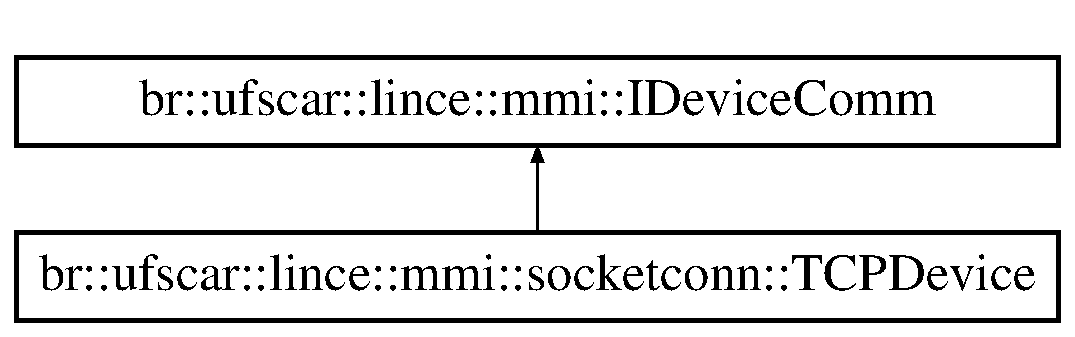
\includegraphics[height=2cm]{classbr_1_1ufscar_1_1lince_1_1mmi_1_1socketconn_1_1TCPDevice}
\end{center}
\end{figure}
\subsection*{Public Member Functions}
\begin{DoxyCompactItemize}
\item 
\hyperlink{classbr_1_1ufscar_1_1lince_1_1mmi_1_1socketconn_1_1TCPDevice_abad8a6e03c83f08d453c45802dbf5d24}{TCPDevice} (\hyperlink{classbr_1_1ufscar_1_1lince_1_1mmi_1_1socketconn_1_1SocketTCP}{SocketTCP} $\ast$socket)
\item 
\hyperlink{classbr_1_1ufscar_1_1lince_1_1mmi_1_1socketconn_1_1TCPDevice_a54143d24714fe38957c7f3432d7f4ddf}{$\sim$TCPDevice} ()
\item 
void \hyperlink{classbr_1_1ufscar_1_1lince_1_1mmi_1_1socketconn_1_1TCPDevice_a2a474f7f39371460268525b0a840cd4f}{connect} ()
\begin{DoxyCompactList}\small\item\em This method stabilishes a connect between the device and the \hyperlink{classbr_1_1ufscar_1_1lince_1_1mmi_1_1MMIManager}{MMIManager}, allowing the device reports his multimodal events. \item\end{DoxyCompactList}\item 
void \hyperlink{classbr_1_1ufscar_1_1lince_1_1mmi_1_1socketconn_1_1TCPDevice_a5b1eca485752195ce49f03475229ca1f}{disconnect} ()
\begin{DoxyCompactList}\small\item\em This method finishes the connection between the devica and \hyperlink{classbr_1_1ufscar_1_1lince_1_1mmi_1_1MMIManager}{MMIManager}. \item\end{DoxyCompactList}\item 
void \hyperlink{classbr_1_1ufscar_1_1lince_1_1mmi_1_1socketconn_1_1TCPDevice_a533e8c0d49d2418a244e46242dc70d99}{sendToDevice} (vector$<$ string $>$ $\ast$args)
\begin{DoxyCompactList}\small\item\em This method allows send a message to the device. \item\end{DoxyCompactList}\item 
string \hyperlink{classbr_1_1ufscar_1_1lince_1_1mmi_1_1socketconn_1_1TCPDevice_aa45bb0937e02c3d58c9923c369408e5a}{getDeviceId} ()
\begin{DoxyCompactList}\small\item\em This method return the id of the device. \item\end{DoxyCompactList}\item 
void \hyperlink{classbr_1_1ufscar_1_1lince_1_1mmi_1_1socketconn_1_1TCPDevice_a4004f2bdb8466c2613654469d0863f78}{release} ()
\begin{DoxyCompactList}\small\item\em This method make the device reset its internals variables. \item\end{DoxyCompactList}\item 
string \hyperlink{classbr_1_1ufscar_1_1lince_1_1mmi_1_1socketconn_1_1TCPDevice_a3d899beea9a5d297ee21931be41684ec}{getDeviceIP} ()
\item 
unsigned short \hyperlink{classbr_1_1ufscar_1_1lince_1_1mmi_1_1socketconn_1_1TCPDevice_a163fd810dccd2682328735a02699372d}{getDevicePort} ()
\end{DoxyCompactItemize}


\subsection{Constructor \& Destructor Documentation}
\hypertarget{classbr_1_1ufscar_1_1lince_1_1mmi_1_1socketconn_1_1TCPDevice_abad8a6e03c83f08d453c45802dbf5d24}{
\index{br::ufscar::lince::mmi::socketconn::TCPDevice@{br::ufscar::lince::mmi::socketconn::TCPDevice}!TCPDevice@{TCPDevice}}
\index{TCPDevice@{TCPDevice}!br::ufscar::lince::mmi::socketconn::TCPDevice@{br::ufscar::lince::mmi::socketconn::TCPDevice}}
\subsubsection[{TCPDevice}]{\setlength{\rightskip}{0pt plus 5cm}br::ufscar::lince::mmi::socketconn::TCPDevice::TCPDevice ({\bf SocketTCP} $\ast$ {\em socket})}}
\label{classbr_1_1ufscar_1_1lince_1_1mmi_1_1socketconn_1_1TCPDevice_abad8a6e03c83f08d453c45802dbf5d24}
\hypertarget{classbr_1_1ufscar_1_1lince_1_1mmi_1_1socketconn_1_1TCPDevice_a54143d24714fe38957c7f3432d7f4ddf}{
\index{br::ufscar::lince::mmi::socketconn::TCPDevice@{br::ufscar::lince::mmi::socketconn::TCPDevice}!$\sim$TCPDevice@{$\sim$TCPDevice}}
\index{$\sim$TCPDevice@{$\sim$TCPDevice}!br::ufscar::lince::mmi::socketconn::TCPDevice@{br::ufscar::lince::mmi::socketconn::TCPDevice}}
\subsubsection[{$\sim$TCPDevice}]{\setlength{\rightskip}{0pt plus 5cm}br::ufscar::lince::mmi::socketconn::TCPDevice::$\sim$TCPDevice ()}}
\label{classbr_1_1ufscar_1_1lince_1_1mmi_1_1socketconn_1_1TCPDevice_a54143d24714fe38957c7f3432d7f4ddf}


\subsection{Member Function Documentation}
\hypertarget{classbr_1_1ufscar_1_1lince_1_1mmi_1_1socketconn_1_1TCPDevice_a2a474f7f39371460268525b0a840cd4f}{
\index{br::ufscar::lince::mmi::socketconn::TCPDevice@{br::ufscar::lince::mmi::socketconn::TCPDevice}!connect@{connect}}
\index{connect@{connect}!br::ufscar::lince::mmi::socketconn::TCPDevice@{br::ufscar::lince::mmi::socketconn::TCPDevice}}
\subsubsection[{connect}]{\setlength{\rightskip}{0pt plus 5cm}void br::ufscar::lince::mmi::socketconn::TCPDevice::connect ()\hspace{0.3cm}{\ttfamily  \mbox{[}virtual\mbox{]}}}}
\label{classbr_1_1ufscar_1_1lince_1_1mmi_1_1socketconn_1_1TCPDevice_a2a474f7f39371460268525b0a840cd4f}


This method stabilishes a connect between the device and the \hyperlink{classbr_1_1ufscar_1_1lince_1_1mmi_1_1MMIManager}{MMIManager}, allowing the device reports his multimodal events. 



Implements \hyperlink{classbr_1_1ufscar_1_1lince_1_1mmi_1_1IDeviceComm_a53f48993f294b9a755125b6ccdb06ad4}{br::ufscar::lince::mmi::IDeviceComm}.

\hypertarget{classbr_1_1ufscar_1_1lince_1_1mmi_1_1socketconn_1_1TCPDevice_a5b1eca485752195ce49f03475229ca1f}{
\index{br::ufscar::lince::mmi::socketconn::TCPDevice@{br::ufscar::lince::mmi::socketconn::TCPDevice}!disconnect@{disconnect}}
\index{disconnect@{disconnect}!br::ufscar::lince::mmi::socketconn::TCPDevice@{br::ufscar::lince::mmi::socketconn::TCPDevice}}
\subsubsection[{disconnect}]{\setlength{\rightskip}{0pt plus 5cm}void br::ufscar::lince::mmi::socketconn::TCPDevice::disconnect ()\hspace{0.3cm}{\ttfamily  \mbox{[}virtual\mbox{]}}}}
\label{classbr_1_1ufscar_1_1lince_1_1mmi_1_1socketconn_1_1TCPDevice_a5b1eca485752195ce49f03475229ca1f}


This method finishes the connection between the devica and \hyperlink{classbr_1_1ufscar_1_1lince_1_1mmi_1_1MMIManager}{MMIManager}. 



Implements \hyperlink{classbr_1_1ufscar_1_1lince_1_1mmi_1_1IDeviceComm_ad3791cf1ab234f4a6b464c3f614c78c6}{br::ufscar::lince::mmi::IDeviceComm}.

\hypertarget{classbr_1_1ufscar_1_1lince_1_1mmi_1_1socketconn_1_1TCPDevice_aa45bb0937e02c3d58c9923c369408e5a}{
\index{br::ufscar::lince::mmi::socketconn::TCPDevice@{br::ufscar::lince::mmi::socketconn::TCPDevice}!getDeviceId@{getDeviceId}}
\index{getDeviceId@{getDeviceId}!br::ufscar::lince::mmi::socketconn::TCPDevice@{br::ufscar::lince::mmi::socketconn::TCPDevice}}
\subsubsection[{getDeviceId}]{\setlength{\rightskip}{0pt plus 5cm}string br::ufscar::lince::mmi::socketconn::TCPDevice::getDeviceId ()\hspace{0.3cm}{\ttfamily  \mbox{[}virtual\mbox{]}}}}
\label{classbr_1_1ufscar_1_1lince_1_1mmi_1_1socketconn_1_1TCPDevice_aa45bb0937e02c3d58c9923c369408e5a}


This method return the id of the device. 

\begin{DoxyReturn}{Returns}
Device identification. 
\end{DoxyReturn}


Implements \hyperlink{classbr_1_1ufscar_1_1lince_1_1mmi_1_1IDeviceComm_a4ae69c19445713ddc9fda351555c1ac2}{br::ufscar::lince::mmi::IDeviceComm}.

\hypertarget{classbr_1_1ufscar_1_1lince_1_1mmi_1_1socketconn_1_1TCPDevice_a3d899beea9a5d297ee21931be41684ec}{
\index{br::ufscar::lince::mmi::socketconn::TCPDevice@{br::ufscar::lince::mmi::socketconn::TCPDevice}!getDeviceIP@{getDeviceIP}}
\index{getDeviceIP@{getDeviceIP}!br::ufscar::lince::mmi::socketconn::TCPDevice@{br::ufscar::lince::mmi::socketconn::TCPDevice}}
\subsubsection[{getDeviceIP}]{\setlength{\rightskip}{0pt plus 5cm}string br::ufscar::lince::mmi::socketconn::TCPDevice::getDeviceIP ()}}
\label{classbr_1_1ufscar_1_1lince_1_1mmi_1_1socketconn_1_1TCPDevice_a3d899beea9a5d297ee21931be41684ec}
\hypertarget{classbr_1_1ufscar_1_1lince_1_1mmi_1_1socketconn_1_1TCPDevice_a163fd810dccd2682328735a02699372d}{
\index{br::ufscar::lince::mmi::socketconn::TCPDevice@{br::ufscar::lince::mmi::socketconn::TCPDevice}!getDevicePort@{getDevicePort}}
\index{getDevicePort@{getDevicePort}!br::ufscar::lince::mmi::socketconn::TCPDevice@{br::ufscar::lince::mmi::socketconn::TCPDevice}}
\subsubsection[{getDevicePort}]{\setlength{\rightskip}{0pt plus 5cm}unsigned short br::ufscar::lince::mmi::socketconn::TCPDevice::getDevicePort ()}}
\label{classbr_1_1ufscar_1_1lince_1_1mmi_1_1socketconn_1_1TCPDevice_a163fd810dccd2682328735a02699372d}
\hypertarget{classbr_1_1ufscar_1_1lince_1_1mmi_1_1socketconn_1_1TCPDevice_a4004f2bdb8466c2613654469d0863f78}{
\index{br::ufscar::lince::mmi::socketconn::TCPDevice@{br::ufscar::lince::mmi::socketconn::TCPDevice}!release@{release}}
\index{release@{release}!br::ufscar::lince::mmi::socketconn::TCPDevice@{br::ufscar::lince::mmi::socketconn::TCPDevice}}
\subsubsection[{release}]{\setlength{\rightskip}{0pt plus 5cm}void br::ufscar::lince::mmi::socketconn::TCPDevice::release ()\hspace{0.3cm}{\ttfamily  \mbox{[}virtual\mbox{]}}}}
\label{classbr_1_1ufscar_1_1lince_1_1mmi_1_1socketconn_1_1TCPDevice_a4004f2bdb8466c2613654469d0863f78}


This method make the device reset its internals variables. 



Implements \hyperlink{classbr_1_1ufscar_1_1lince_1_1mmi_1_1IDeviceComm_a9c173ebb83a502e78143a52fc7d87a80}{br::ufscar::lince::mmi::IDeviceComm}.

\hypertarget{classbr_1_1ufscar_1_1lince_1_1mmi_1_1socketconn_1_1TCPDevice_a533e8c0d49d2418a244e46242dc70d99}{
\index{br::ufscar::lince::mmi::socketconn::TCPDevice@{br::ufscar::lince::mmi::socketconn::TCPDevice}!sendToDevice@{sendToDevice}}
\index{sendToDevice@{sendToDevice}!br::ufscar::lince::mmi::socketconn::TCPDevice@{br::ufscar::lince::mmi::socketconn::TCPDevice}}
\subsubsection[{sendToDevice}]{\setlength{\rightskip}{0pt plus 5cm}void br::ufscar::lince::mmi::socketconn::TCPDevice::sendToDevice (vector$<$ string $>$ $\ast$ {\em args})\hspace{0.3cm}{\ttfamily  \mbox{[}virtual\mbox{]}}}}
\label{classbr_1_1ufscar_1_1lince_1_1mmi_1_1socketconn_1_1TCPDevice_a533e8c0d49d2418a244e46242dc70d99}


This method allows send a message to the device. 


\begin{DoxyParams}{Parameters}
\item[{\em args}]A array of strings that will contain the message. \end{DoxyParams}


Implements \hyperlink{classbr_1_1ufscar_1_1lince_1_1mmi_1_1IDeviceComm_a0249a13030b4df9b50778723421375d9}{br::ufscar::lince::mmi::IDeviceComm}.



The documentation for this class was generated from the following file:\begin{DoxyCompactItemize}
\item 
include/socketconn/\hyperlink{TCPDevice_8h}{TCPDevice.h}\end{DoxyCompactItemize}

\hypertarget{classbr_1_1ufscar_1_1lince_1_1mmi_1_1ink_1_1Trace}{
\section{br::ufscar::lince::mmi::ink::Trace Class Reference}
\label{classbr_1_1ufscar_1_1lince_1_1mmi_1_1ink_1_1Trace}\index{br::ufscar::lince::mmi::ink::Trace@{br::ufscar::lince::mmi::ink::Trace}}
}


Classe que representa um trace de um InkML.  




{\ttfamily \#include $<$Trace.h$>$}

\subsection*{Public Member Functions}
\begin{DoxyCompactItemize}
\item 
\hyperlink{classbr_1_1ufscar_1_1lince_1_1mmi_1_1ink_1_1Trace_a87eb33bfb0d672cb8b15e05596c2d185}{Trace} ()
\begin{DoxyCompactList}\small\item\em Desc -\/ constructor. \item\end{DoxyCompactList}\item 
void \hyperlink{classbr_1_1ufscar_1_1lince_1_1mmi_1_1ink_1_1Trace_a2a65005bfc41352c9c9253eef966e8e7}{setTraceFormatRef} (\hyperlink{classbr_1_1ufscar_1_1lince_1_1mmi_1_1ink_1_1TraceFormat}{TraceFormat} $\ast$\hyperlink{classbr_1_1ufscar_1_1lince_1_1mmi_1_1ink_1_1Trace_a87c33c99c915d0ae5808adf580554c42}{traceFormatRef})
\begin{DoxyCompactList}\small\item\em Desc -\/ assign traceFormat of this trace. \item\end{DoxyCompactList}\item 
void \hyperlink{classbr_1_1ufscar_1_1lince_1_1mmi_1_1ink_1_1Trace_aec507a4fd35f2fd65dedc3a4cd168064}{parseTraceData} (char $\ast$data, \hyperlink{structbr_1_1ufscar_1_1lince_1_1mmi_1_1ink_1_1structBoundingBox}{BoundingBox} $\ast$boundingBox)
\end{DoxyCompactItemize}
\subsection*{Data Fields}
\begin{DoxyCompactItemize}
\item 
\hyperlink{classbr_1_1ufscar_1_1lince_1_1mmi_1_1ink_1_1TraceFormat}{TraceFormat} $\ast$ \hyperlink{classbr_1_1ufscar_1_1lince_1_1mmi_1_1ink_1_1Trace_a87c33c99c915d0ae5808adf580554c42}{traceFormatRef}
\begin{DoxyCompactList}\small\item\em Desc -\/ Reference to the associated \hyperlink{classbr_1_1ufscar_1_1lince_1_1mmi_1_1ink_1_1TraceFormat}{TraceFormat}. \item\end{DoxyCompactList}\item 
vector$<$ long $>$ $\ast$ \hyperlink{classbr_1_1ufscar_1_1lince_1_1mmi_1_1ink_1_1Trace_a9a8d9f9bbffdd49af980bdd7c80ee4ae}{vectX}
\begin{DoxyCompactList}\small\item\em Desc -\/ To hold channel X data (i.e. \item\end{DoxyCompactList}\item 
vector$<$ long $>$ $\ast$ \hyperlink{classbr_1_1ufscar_1_1lince_1_1mmi_1_1ink_1_1Trace_a6914065da435b344151f55f6d60a7fdd}{vectY}
\begin{DoxyCompactList}\small\item\em Desc -\/ To hold channel Y data (i.e. \item\end{DoxyCompactList}\item 
vector$<$ int $>$ $\ast$ \hyperlink{classbr_1_1ufscar_1_1lince_1_1mmi_1_1ink_1_1Trace_ab73af23278fce63da5defb36a2bc5cea}{vectF}
\begin{DoxyCompactList}\small\item\em Desc -\/ To hold channel F data (i.e. \item\end{DoxyCompactList}\end{DoxyCompactItemize}


\subsection{Detailed Description}
Classe que representa um trace de um InkML. Mais informações em \href{http://sourceforge.net/apps/trac/inkmltk/wiki/InkMLLib}{\tt http://sourceforge.net/apps/trac/inkmltk/wiki/InkMLLib} 

\subsection{Constructor \& Destructor Documentation}
\hypertarget{classbr_1_1ufscar_1_1lince_1_1mmi_1_1ink_1_1Trace_a87eb33bfb0d672cb8b15e05596c2d185}{
\index{br::ufscar::lince::mmi::ink::Trace@{br::ufscar::lince::mmi::ink::Trace}!Trace@{Trace}}
\index{Trace@{Trace}!br::ufscar::lince::mmi::ink::Trace@{br::ufscar::lince::mmi::ink::Trace}}
\subsubsection[{Trace}]{\setlength{\rightskip}{0pt plus 5cm}br::ufscar::lince::mmi::ink::Trace::Trace ()}}
\label{classbr_1_1ufscar_1_1lince_1_1mmi_1_1ink_1_1Trace_a87eb33bfb0d672cb8b15e05596c2d185}


Desc -\/ constructor. 



\subsection{Member Function Documentation}
\hypertarget{classbr_1_1ufscar_1_1lince_1_1mmi_1_1ink_1_1Trace_aec507a4fd35f2fd65dedc3a4cd168064}{
\index{br::ufscar::lince::mmi::ink::Trace@{br::ufscar::lince::mmi::ink::Trace}!parseTraceData@{parseTraceData}}
\index{parseTraceData@{parseTraceData}!br::ufscar::lince::mmi::ink::Trace@{br::ufscar::lince::mmi::ink::Trace}}
\subsubsection[{parseTraceData}]{\setlength{\rightskip}{0pt plus 5cm}void br::ufscar::lince::mmi::ink::Trace::parseTraceData (char $\ast$ {\em data}, \/  {\bf BoundingBox} $\ast$ {\em boundingBox})}}
\label{classbr_1_1ufscar_1_1lince_1_1mmi_1_1ink_1_1Trace_aec507a4fd35f2fd65dedc3a4cd168064}
\hypertarget{classbr_1_1ufscar_1_1lince_1_1mmi_1_1ink_1_1Trace_a2a65005bfc41352c9c9253eef966e8e7}{
\index{br::ufscar::lince::mmi::ink::Trace@{br::ufscar::lince::mmi::ink::Trace}!setTraceFormatRef@{setTraceFormatRef}}
\index{setTraceFormatRef@{setTraceFormatRef}!br::ufscar::lince::mmi::ink::Trace@{br::ufscar::lince::mmi::ink::Trace}}
\subsubsection[{setTraceFormatRef}]{\setlength{\rightskip}{0pt plus 5cm}void br::ufscar::lince::mmi::ink::Trace::setTraceFormatRef ({\bf TraceFormat} $\ast$ {\em traceFormatRef})\hspace{0.3cm}{\ttfamily  \mbox{[}inline\mbox{]}}}}
\label{classbr_1_1ufscar_1_1lince_1_1mmi_1_1ink_1_1Trace_a2a65005bfc41352c9c9253eef966e8e7}


Desc -\/ assign traceFormat of this trace. 



\subsection{Field Documentation}
\hypertarget{classbr_1_1ufscar_1_1lince_1_1mmi_1_1ink_1_1Trace_a87c33c99c915d0ae5808adf580554c42}{
\index{br::ufscar::lince::mmi::ink::Trace@{br::ufscar::lince::mmi::ink::Trace}!traceFormatRef@{traceFormatRef}}
\index{traceFormatRef@{traceFormatRef}!br::ufscar::lince::mmi::ink::Trace@{br::ufscar::lince::mmi::ink::Trace}}
\subsubsection[{traceFormatRef}]{\setlength{\rightskip}{0pt plus 5cm}{\bf TraceFormat}$\ast$ {\bf br::ufscar::lince::mmi::ink::Trace::traceFormatRef}}}
\label{classbr_1_1ufscar_1_1lince_1_1mmi_1_1ink_1_1Trace_a87c33c99c915d0ae5808adf580554c42}


Desc -\/ Reference to the associated \hyperlink{classbr_1_1ufscar_1_1lince_1_1mmi_1_1ink_1_1TraceFormat}{TraceFormat}. 

\hypertarget{classbr_1_1ufscar_1_1lince_1_1mmi_1_1ink_1_1Trace_ab73af23278fce63da5defb36a2bc5cea}{
\index{br::ufscar::lince::mmi::ink::Trace@{br::ufscar::lince::mmi::ink::Trace}!vectF@{vectF}}
\index{vectF@{vectF}!br::ufscar::lince::mmi::ink::Trace@{br::ufscar::lince::mmi::ink::Trace}}
\subsubsection[{vectF}]{\setlength{\rightskip}{0pt plus 5cm}vector$<$int$>$$\ast$ {\bf br::ufscar::lince::mmi::ink::Trace::vectF}}}
\label{classbr_1_1ufscar_1_1lince_1_1mmi_1_1ink_1_1Trace_ab73af23278fce63da5defb36a2bc5cea}


Desc -\/ To hold channel F data (i.e. 

Pressure/Force co-\/ordinate data). \hypertarget{classbr_1_1ufscar_1_1lince_1_1mmi_1_1ink_1_1Trace_a9a8d9f9bbffdd49af980bdd7c80ee4ae}{
\index{br::ufscar::lince::mmi::ink::Trace@{br::ufscar::lince::mmi::ink::Trace}!vectX@{vectX}}
\index{vectX@{vectX}!br::ufscar::lince::mmi::ink::Trace@{br::ufscar::lince::mmi::ink::Trace}}
\subsubsection[{vectX}]{\setlength{\rightskip}{0pt plus 5cm}vector$<$long$>$$\ast$ {\bf br::ufscar::lince::mmi::ink::Trace::vectX}}}
\label{classbr_1_1ufscar_1_1lince_1_1mmi_1_1ink_1_1Trace_a9a8d9f9bbffdd49af980bdd7c80ee4ae}


Desc -\/ To hold channel X data (i.e. 

X co-\/ordinate data). \hypertarget{classbr_1_1ufscar_1_1lince_1_1mmi_1_1ink_1_1Trace_a6914065da435b344151f55f6d60a7fdd}{
\index{br::ufscar::lince::mmi::ink::Trace@{br::ufscar::lince::mmi::ink::Trace}!vectY@{vectY}}
\index{vectY@{vectY}!br::ufscar::lince::mmi::ink::Trace@{br::ufscar::lince::mmi::ink::Trace}}
\subsubsection[{vectY}]{\setlength{\rightskip}{0pt plus 5cm}vector$<$long$>$$\ast$ {\bf br::ufscar::lince::mmi::ink::Trace::vectY}}}
\label{classbr_1_1ufscar_1_1lince_1_1mmi_1_1ink_1_1Trace_a6914065da435b344151f55f6d60a7fdd}


Desc -\/ To hold channel Y data (i.e. 

Y co-\/ordinate data). 

The documentation for this class was generated from the following file:\begin{DoxyCompactItemize}
\item 
include/ink/\hyperlink{Trace_8h}{Trace.h}\end{DoxyCompactItemize}

\hypertarget{classbr_1_1ufscar_1_1lince_1_1mmi_1_1ink_1_1TraceFormat}{
\section{br::ufscar::lince::mmi::ink::TraceFormat Class Reference}
\label{classbr_1_1ufscar_1_1lince_1_1mmi_1_1ink_1_1TraceFormat}\index{br::ufscar::lince::mmi::ink::TraceFormat@{br::ufscar::lince::mmi::ink::TraceFormat}}
}


Classe que representa o formato de um trace de um InkML.  




{\ttfamily \#include $<$TraceFormat.h$>$}

\subsection*{Public Member Functions}
\begin{DoxyCompactItemize}
\item 
\hyperlink{classbr_1_1ufscar_1_1lince_1_1mmi_1_1ink_1_1TraceFormat_a94ab4a2d743d17fb14c2af98a62b0550}{TraceFormat} ()
\begin{DoxyCompactList}\small\item\em Desc -\/ Constructor. \item\end{DoxyCompactList}\item 
\hyperlink{classbr_1_1ufscar_1_1lince_1_1mmi_1_1ink_1_1TraceFormat_ae3d05ea0cfd71e7af419ddc36b05cdc8}{TraceFormat} (char $\ast$\hyperlink{classbr_1_1ufscar_1_1lince_1_1mmi_1_1ink_1_1TraceFormat_ad89fcbbb40fb5691df020fa57b325f44}{id})
\begin{DoxyCompactList}\small\item\em Construtor. \item\end{DoxyCompactList}\item 
void \hyperlink{classbr_1_1ufscar_1_1lince_1_1mmi_1_1ink_1_1TraceFormat_a4f21a24e009159e4062f2a2a47cc68fc}{addChannelOrder} (\hyperlink{namespacebr_1_1ufscar_1_1lince_1_1mmi_1_1ink_a857f7b80c5d28f256c70d78cacf91dab}{CHANNEL} c)
\begin{DoxyCompactList}\small\item\em Adiciona um channel. \item\end{DoxyCompactList}\item 
char $\ast$ \hyperlink{classbr_1_1ufscar_1_1lince_1_1mmi_1_1ink_1_1TraceFormat_afc72b9eb02901fb2a58c159b73231c6a}{getID} ()
\begin{DoxyCompactList}\small\item\em Acessa o ID do traceFormat. \item\end{DoxyCompactList}\item 
\hyperlink{namespacebr_1_1ufscar_1_1lince_1_1mmi_1_1ink_a857f7b80c5d28f256c70d78cacf91dab}{CHANNEL} \hyperlink{classbr_1_1ufscar_1_1lince_1_1mmi_1_1ink_1_1TraceFormat_af6c038f7182928e11aedafe61a7f1af0}{getChannelAtIndex} (int index)
\begin{DoxyCompactList}\small\item\em Acessa um determinado channel. \item\end{DoxyCompactList}\item 
void \hyperlink{classbr_1_1ufscar_1_1lince_1_1mmi_1_1ink_1_1TraceFormat_a5427bd1c07566f405591f38dfd2ec5f9}{addChannelOrder} (char $\ast$c)
\begin{DoxyCompactList}\small\item\em Adiciona um channel. \item\end{DoxyCompactList}\end{DoxyCompactItemize}
\subsection*{Data Fields}
\begin{DoxyCompactItemize}
\item 
char $\ast$ \hyperlink{classbr_1_1ufscar_1_1lince_1_1mmi_1_1ink_1_1TraceFormat_ad89fcbbb40fb5691df020fa57b325f44}{id}
\begin{DoxyCompactList}\small\item\em Id do traceFormat. \item\end{DoxyCompactList}\item 
bool \hyperlink{classbr_1_1ufscar_1_1lince_1_1mmi_1_1ink_1_1TraceFormat_ab503ce06d24067ab5f7611793116160e}{channelFPresent}
\begin{DoxyCompactList}\small\item\em Desc -\/ By default only X and Y channels are present This flag is to know whether pressure is present or not. \item\end{DoxyCompactList}\item 
vector$<$ Channel $>$ $\ast$ \hyperlink{classbr_1_1ufscar_1_1lince_1_1mmi_1_1ink_1_1TraceFormat_a7a441396c4a7f0d3a0d05bff74495f37}{vectChannel}
\begin{DoxyCompactList}\small\item\em Lista de channels. \item\end{DoxyCompactList}\item 
vector$<$ \hyperlink{namespacebr_1_1ufscar_1_1lince_1_1mmi_1_1ink_a857f7b80c5d28f256c70d78cacf91dab}{CHANNEL} $>$ $\ast$ \hyperlink{classbr_1_1ufscar_1_1lince_1_1mmi_1_1ink_1_1TraceFormat_ab69e1f7711dde259cb5ef481d025f556}{vectChannelOrder}
\begin{DoxyCompactList}\small\item\em Lista de channels. \item\end{DoxyCompactList}\end{DoxyCompactItemize}


\subsection{Detailed Description}
Classe que representa o formato de um trace de um InkML. Mais informações em \href{http://sourceforge.net/apps/trac/inkmltk/wiki/InkMLLib}{\tt http://sourceforge.net/apps/trac/inkmltk/wiki/InkMLLib} 

\subsection{Constructor \& Destructor Documentation}
\hypertarget{classbr_1_1ufscar_1_1lince_1_1mmi_1_1ink_1_1TraceFormat_a94ab4a2d743d17fb14c2af98a62b0550}{
\index{br::ufscar::lince::mmi::ink::TraceFormat@{br::ufscar::lince::mmi::ink::TraceFormat}!TraceFormat@{TraceFormat}}
\index{TraceFormat@{TraceFormat}!br::ufscar::lince::mmi::ink::TraceFormat@{br::ufscar::lince::mmi::ink::TraceFormat}}
\subsubsection[{TraceFormat}]{\setlength{\rightskip}{0pt plus 5cm}br::ufscar::lince::mmi::ink::TraceFormat::TraceFormat ()}}
\label{classbr_1_1ufscar_1_1lince_1_1mmi_1_1ink_1_1TraceFormat_a94ab4a2d743d17fb14c2af98a62b0550}


Desc -\/ Constructor. 

\hypertarget{classbr_1_1ufscar_1_1lince_1_1mmi_1_1ink_1_1TraceFormat_ae3d05ea0cfd71e7af419ddc36b05cdc8}{
\index{br::ufscar::lince::mmi::ink::TraceFormat@{br::ufscar::lince::mmi::ink::TraceFormat}!TraceFormat@{TraceFormat}}
\index{TraceFormat@{TraceFormat}!br::ufscar::lince::mmi::ink::TraceFormat@{br::ufscar::lince::mmi::ink::TraceFormat}}
\subsubsection[{TraceFormat}]{\setlength{\rightskip}{0pt plus 5cm}br::ufscar::lince::mmi::ink::TraceFormat::TraceFormat (char $\ast$ {\em id})}}
\label{classbr_1_1ufscar_1_1lince_1_1mmi_1_1ink_1_1TraceFormat_ae3d05ea0cfd71e7af419ddc36b05cdc8}


Construtor. 


\begin{DoxyParams}{Parameters}
\item[{\em id}]do traceFormat. \end{DoxyParams}


\subsection{Member Function Documentation}
\hypertarget{classbr_1_1ufscar_1_1lince_1_1mmi_1_1ink_1_1TraceFormat_a5427bd1c07566f405591f38dfd2ec5f9}{
\index{br::ufscar::lince::mmi::ink::TraceFormat@{br::ufscar::lince::mmi::ink::TraceFormat}!addChannelOrder@{addChannelOrder}}
\index{addChannelOrder@{addChannelOrder}!br::ufscar::lince::mmi::ink::TraceFormat@{br::ufscar::lince::mmi::ink::TraceFormat}}
\subsubsection[{addChannelOrder}]{\setlength{\rightskip}{0pt plus 5cm}void br::ufscar::lince::mmi::ink::TraceFormat::addChannelOrder (char $\ast$ {\em c})}}
\label{classbr_1_1ufscar_1_1lince_1_1mmi_1_1ink_1_1TraceFormat_a5427bd1c07566f405591f38dfd2ec5f9}


Adiciona um channel. 


\begin{DoxyParams}{Parameters}
\item[{\em c}]Channel a ser adicionado. \end{DoxyParams}
\hypertarget{classbr_1_1ufscar_1_1lince_1_1mmi_1_1ink_1_1TraceFormat_a4f21a24e009159e4062f2a2a47cc68fc}{
\index{br::ufscar::lince::mmi::ink::TraceFormat@{br::ufscar::lince::mmi::ink::TraceFormat}!addChannelOrder@{addChannelOrder}}
\index{addChannelOrder@{addChannelOrder}!br::ufscar::lince::mmi::ink::TraceFormat@{br::ufscar::lince::mmi::ink::TraceFormat}}
\subsubsection[{addChannelOrder}]{\setlength{\rightskip}{0pt plus 5cm}void br::ufscar::lince::mmi::ink::TraceFormat::addChannelOrder ({\bf CHANNEL} {\em c})\hspace{0.3cm}{\ttfamily  \mbox{[}inline\mbox{]}}}}
\label{classbr_1_1ufscar_1_1lince_1_1mmi_1_1ink_1_1TraceFormat_a4f21a24e009159e4062f2a2a47cc68fc}


Adiciona um channel. 


\begin{DoxyParams}{Parameters}
\item[{\em c}]Channel a ser adicionado. \end{DoxyParams}
\hypertarget{classbr_1_1ufscar_1_1lince_1_1mmi_1_1ink_1_1TraceFormat_af6c038f7182928e11aedafe61a7f1af0}{
\index{br::ufscar::lince::mmi::ink::TraceFormat@{br::ufscar::lince::mmi::ink::TraceFormat}!getChannelAtIndex@{getChannelAtIndex}}
\index{getChannelAtIndex@{getChannelAtIndex}!br::ufscar::lince::mmi::ink::TraceFormat@{br::ufscar::lince::mmi::ink::TraceFormat}}
\subsubsection[{getChannelAtIndex}]{\setlength{\rightskip}{0pt plus 5cm}{\bf CHANNEL} br::ufscar::lince::mmi::ink::TraceFormat::getChannelAtIndex (int {\em index})}}
\label{classbr_1_1ufscar_1_1lince_1_1mmi_1_1ink_1_1TraceFormat_af6c038f7182928e11aedafe61a7f1af0}


Acessa um determinado channel. 


\begin{DoxyParams}{Parameters}
\item[{\em index}]Índice do channel a ser acessado \end{DoxyParams}
\begin{DoxyReturn}{Returns}
O channel 
\end{DoxyReturn}
\hypertarget{classbr_1_1ufscar_1_1lince_1_1mmi_1_1ink_1_1TraceFormat_afc72b9eb02901fb2a58c159b73231c6a}{
\index{br::ufscar::lince::mmi::ink::TraceFormat@{br::ufscar::lince::mmi::ink::TraceFormat}!getID@{getID}}
\index{getID@{getID}!br::ufscar::lince::mmi::ink::TraceFormat@{br::ufscar::lince::mmi::ink::TraceFormat}}
\subsubsection[{getID}]{\setlength{\rightskip}{0pt plus 5cm}char$\ast$ br::ufscar::lince::mmi::ink::TraceFormat::getID ()\hspace{0.3cm}{\ttfamily  \mbox{[}inline\mbox{]}}}}
\label{classbr_1_1ufscar_1_1lince_1_1mmi_1_1ink_1_1TraceFormat_afc72b9eb02901fb2a58c159b73231c6a}


Acessa o ID do traceFormat. 

\begin{DoxyReturn}{Returns}
id do traceFormat. 
\end{DoxyReturn}


\subsection{Field Documentation}
\hypertarget{classbr_1_1ufscar_1_1lince_1_1mmi_1_1ink_1_1TraceFormat_ab503ce06d24067ab5f7611793116160e}{
\index{br::ufscar::lince::mmi::ink::TraceFormat@{br::ufscar::lince::mmi::ink::TraceFormat}!channelFPresent@{channelFPresent}}
\index{channelFPresent@{channelFPresent}!br::ufscar::lince::mmi::ink::TraceFormat@{br::ufscar::lince::mmi::ink::TraceFormat}}
\subsubsection[{channelFPresent}]{\setlength{\rightskip}{0pt plus 5cm}bool {\bf br::ufscar::lince::mmi::ink::TraceFormat::channelFPresent}}}
\label{classbr_1_1ufscar_1_1lince_1_1mmi_1_1ink_1_1TraceFormat_ab503ce06d24067ab5f7611793116160e}


Desc -\/ By default only X and Y channels are present This flag is to know whether pressure is present or not. 

\hypertarget{classbr_1_1ufscar_1_1lince_1_1mmi_1_1ink_1_1TraceFormat_ad89fcbbb40fb5691df020fa57b325f44}{
\index{br::ufscar::lince::mmi::ink::TraceFormat@{br::ufscar::lince::mmi::ink::TraceFormat}!id@{id}}
\index{id@{id}!br::ufscar::lince::mmi::ink::TraceFormat@{br::ufscar::lince::mmi::ink::TraceFormat}}
\subsubsection[{id}]{\setlength{\rightskip}{0pt plus 5cm}char$\ast$ {\bf br::ufscar::lince::mmi::ink::TraceFormat::id}}}
\label{classbr_1_1ufscar_1_1lince_1_1mmi_1_1ink_1_1TraceFormat_ad89fcbbb40fb5691df020fa57b325f44}


Id do traceFormat. 

\hypertarget{classbr_1_1ufscar_1_1lince_1_1mmi_1_1ink_1_1TraceFormat_a7a441396c4a7f0d3a0d05bff74495f37}{
\index{br::ufscar::lince::mmi::ink::TraceFormat@{br::ufscar::lince::mmi::ink::TraceFormat}!vectChannel@{vectChannel}}
\index{vectChannel@{vectChannel}!br::ufscar::lince::mmi::ink::TraceFormat@{br::ufscar::lince::mmi::ink::TraceFormat}}
\subsubsection[{vectChannel}]{\setlength{\rightskip}{0pt plus 5cm}vector$<$Channel$>$$\ast$ {\bf br::ufscar::lince::mmi::ink::TraceFormat::vectChannel}}}
\label{classbr_1_1ufscar_1_1lince_1_1mmi_1_1ink_1_1TraceFormat_a7a441396c4a7f0d3a0d05bff74495f37}


Lista de channels. 

\hypertarget{classbr_1_1ufscar_1_1lince_1_1mmi_1_1ink_1_1TraceFormat_ab69e1f7711dde259cb5ef481d025f556}{
\index{br::ufscar::lince::mmi::ink::TraceFormat@{br::ufscar::lince::mmi::ink::TraceFormat}!vectChannelOrder@{vectChannelOrder}}
\index{vectChannelOrder@{vectChannelOrder}!br::ufscar::lince::mmi::ink::TraceFormat@{br::ufscar::lince::mmi::ink::TraceFormat}}
\subsubsection[{vectChannelOrder}]{\setlength{\rightskip}{0pt plus 5cm}vector$<${\bf CHANNEL}$>$$\ast$ {\bf br::ufscar::lince::mmi::ink::TraceFormat::vectChannelOrder}}}
\label{classbr_1_1ufscar_1_1lince_1_1mmi_1_1ink_1_1TraceFormat_ab69e1f7711dde259cb5ef481d025f556}


Lista de channels. 



The documentation for this class was generated from the following file:\begin{DoxyCompactItemize}
\item 
include/ink/\hyperlink{TraceFormat_8h}{TraceFormat.h}\end{DoxyCompactItemize}

\hypertarget{classbr_1_1ufscar_1_1lince_1_1mmi_1_1wii_1_1WiiButtonReport}{
\section{br::ufscar::lince::mmi::wii::WiiButtonReport Class Reference}
\label{classbr_1_1ufscar_1_1lince_1_1mmi_1_1wii_1_1WiiButtonReport}\index{br::ufscar::lince::mmi::wii::WiiButtonReport@{br::ufscar::lince::mmi::wii::WiiButtonReport}}
}


{\ttfamily \#include $<$WiiButtonReport.h$>$}

\subsection*{Public Member Functions}
\begin{DoxyCompactItemize}
\item 
\hyperlink{classbr_1_1ufscar_1_1lince_1_1mmi_1_1wii_1_1WiiButtonReport_a7e958fef164118ccacbe8cd4eb7d3708}{WiiButtonReport} (string deviceId, \hyperlink{classbr_1_1ufscar_1_1lince_1_1mmi_1_1wii_1_1WiiEventHandler}{WiiEventHandler} $\ast$handler, \hyperlink{classbr_1_1ufscar_1_1lince_1_1mmi_1_1wii_1_1WiiDriver}{WiiDriver} $\ast$wiiDriver)
\item 
\hyperlink{classbr_1_1ufscar_1_1lince_1_1mmi_1_1wii_1_1WiiButtonReport_a381456e6d72e3bf8503af0be300c7087}{$\sim$WiiButtonReport} ()
\item 
virtual void \hyperlink{classbr_1_1ufscar_1_1lince_1_1mmi_1_1wii_1_1WiiButtonReport_a18c5cdabeb267b938b289249cb134016}{run} ()
\end{DoxyCompactItemize}


\subsection{Constructor \& Destructor Documentation}
\hypertarget{classbr_1_1ufscar_1_1lince_1_1mmi_1_1wii_1_1WiiButtonReport_a7e958fef164118ccacbe8cd4eb7d3708}{
\index{br::ufscar::lince::mmi::wii::WiiButtonReport@{br::ufscar::lince::mmi::wii::WiiButtonReport}!WiiButtonReport@{WiiButtonReport}}
\index{WiiButtonReport@{WiiButtonReport}!br::ufscar::lince::mmi::wii::WiiButtonReport@{br::ufscar::lince::mmi::wii::WiiButtonReport}}
\subsubsection[{WiiButtonReport}]{\setlength{\rightskip}{0pt plus 5cm}br::ufscar::lince::mmi::wii::WiiButtonReport::WiiButtonReport (string {\em deviceId}, \/  {\bf WiiEventHandler} $\ast$ {\em handler}, \/  {\bf WiiDriver} $\ast$ {\em wiiDriver})}}
\label{classbr_1_1ufscar_1_1lince_1_1mmi_1_1wii_1_1WiiButtonReport_a7e958fef164118ccacbe8cd4eb7d3708}
\hypertarget{classbr_1_1ufscar_1_1lince_1_1mmi_1_1wii_1_1WiiButtonReport_a381456e6d72e3bf8503af0be300c7087}{
\index{br::ufscar::lince::mmi::wii::WiiButtonReport@{br::ufscar::lince::mmi::wii::WiiButtonReport}!$\sim$WiiButtonReport@{$\sim$WiiButtonReport}}
\index{$\sim$WiiButtonReport@{$\sim$WiiButtonReport}!br::ufscar::lince::mmi::wii::WiiButtonReport@{br::ufscar::lince::mmi::wii::WiiButtonReport}}
\subsubsection[{$\sim$WiiButtonReport}]{\setlength{\rightskip}{0pt plus 5cm}br::ufscar::lince::mmi::wii::WiiButtonReport::$\sim$WiiButtonReport ()}}
\label{classbr_1_1ufscar_1_1lince_1_1mmi_1_1wii_1_1WiiButtonReport_a381456e6d72e3bf8503af0be300c7087}


\subsection{Member Function Documentation}
\hypertarget{classbr_1_1ufscar_1_1lince_1_1mmi_1_1wii_1_1WiiButtonReport_a18c5cdabeb267b938b289249cb134016}{
\index{br::ufscar::lince::mmi::wii::WiiButtonReport@{br::ufscar::lince::mmi::wii::WiiButtonReport}!run@{run}}
\index{run@{run}!br::ufscar::lince::mmi::wii::WiiButtonReport@{br::ufscar::lince::mmi::wii::WiiButtonReport}}
\subsubsection[{run}]{\setlength{\rightskip}{0pt plus 5cm}virtual void br::ufscar::lince::mmi::wii::WiiButtonReport::run ()\hspace{0.3cm}{\ttfamily  \mbox{[}virtual\mbox{]}}}}
\label{classbr_1_1ufscar_1_1lince_1_1mmi_1_1wii_1_1WiiButtonReport_a18c5cdabeb267b938b289249cb134016}


The documentation for this class was generated from the following file:\begin{DoxyCompactItemize}
\item 
include/wii/\hyperlink{WiiButtonReport_8h}{WiiButtonReport.h}\end{DoxyCompactItemize}

\hypertarget{classbr_1_1ufscar_1_1lince_1_1mmi_1_1wii_1_1WiiDriver}{
\section{br::ufscar::lince::mmi::wii::WiiDriver Class Reference}
\label{classbr_1_1ufscar_1_1lince_1_1mmi_1_1wii_1_1WiiDriver}\index{br::ufscar::lince::mmi::wii::WiiDriver@{br::ufscar::lince::mmi::wii::WiiDriver}}
}


{\ttfamily \#include $<$WiiDriver.h$>$}

\subsection*{Public Member Functions}
\begin{DoxyCompactItemize}
\item 
\hyperlink{classbr_1_1ufscar_1_1lince_1_1mmi_1_1wii_1_1WiiDriver_aab5fa49a7f90c20ea316a912c5b335fc}{WiiDriver} ()
\item 
virtual \hyperlink{classbr_1_1ufscar_1_1lince_1_1mmi_1_1wii_1_1WiiDriver_afec30a49896ecbfdef96b7043fa2a799}{$\sim$WiiDriver} ()
\item 
\hyperlink{classbr_1_1ufscar_1_1lince_1_1mmi_1_1wii_1_1WiiState}{WiiState} $\ast$ \hyperlink{classbr_1_1ufscar_1_1lince_1_1mmi_1_1wii_1_1WiiDriver_ad1fbb26cfd5009f792d7ad7f23b42523}{getCurrentState} ()
\item 
bool \hyperlink{classbr_1_1ufscar_1_1lince_1_1mmi_1_1wii_1_1WiiDriver_ad1fb0372f607385c3b20391eb005212d}{isButtonsSetted} ()
\item 
bool \hyperlink{classbr_1_1ufscar_1_1lince_1_1mmi_1_1wii_1_1WiiDriver_a8f54679e95645ad0284d77c51987ab98}{isAccelerometerSetted} ()
\item 
bool \hyperlink{classbr_1_1ufscar_1_1lince_1_1mmi_1_1wii_1_1WiiDriver_a419b13cbd01d04d9399287ce643c7b04}{isInfraredSetted} ()
\item 
void \hyperlink{classbr_1_1ufscar_1_1lince_1_1mmi_1_1wii_1_1WiiDriver_a24c5e0a9b6067419be8c08e8519b698f}{setButtons} (bool b)
\item 
void \hyperlink{classbr_1_1ufscar_1_1lince_1_1mmi_1_1wii_1_1WiiDriver_a98c084d2c015c259c252e72958afc986}{setAccelerometer} (bool b)
\item 
void \hyperlink{classbr_1_1ufscar_1_1lince_1_1mmi_1_1wii_1_1WiiDriver_a71196f296c892a1d8874da0d8eef9734}{setInfrared} (bool b)
\item 
void \hyperlink{classbr_1_1ufscar_1_1lince_1_1mmi_1_1wii_1_1WiiDriver_af383ae86791787d26b0bc3f817fb4146}{connect} ()
\end{DoxyCompactItemize}


\subsection{Constructor \& Destructor Documentation}
\hypertarget{classbr_1_1ufscar_1_1lince_1_1mmi_1_1wii_1_1WiiDriver_aab5fa49a7f90c20ea316a912c5b335fc}{
\index{br::ufscar::lince::mmi::wii::WiiDriver@{br::ufscar::lince::mmi::wii::WiiDriver}!WiiDriver@{WiiDriver}}
\index{WiiDriver@{WiiDriver}!br::ufscar::lince::mmi::wii::WiiDriver@{br::ufscar::lince::mmi::wii::WiiDriver}}
\subsubsection[{WiiDriver}]{\setlength{\rightskip}{0pt plus 5cm}br::ufscar::lince::mmi::wii::WiiDriver::WiiDriver ()}}
\label{classbr_1_1ufscar_1_1lince_1_1mmi_1_1wii_1_1WiiDriver_aab5fa49a7f90c20ea316a912c5b335fc}
\hypertarget{classbr_1_1ufscar_1_1lince_1_1mmi_1_1wii_1_1WiiDriver_afec30a49896ecbfdef96b7043fa2a799}{
\index{br::ufscar::lince::mmi::wii::WiiDriver@{br::ufscar::lince::mmi::wii::WiiDriver}!$\sim$WiiDriver@{$\sim$WiiDriver}}
\index{$\sim$WiiDriver@{$\sim$WiiDriver}!br::ufscar::lince::mmi::wii::WiiDriver@{br::ufscar::lince::mmi::wii::WiiDriver}}
\subsubsection[{$\sim$WiiDriver}]{\setlength{\rightskip}{0pt plus 5cm}virtual br::ufscar::lince::mmi::wii::WiiDriver::$\sim$WiiDriver ()\hspace{0.3cm}{\ttfamily  \mbox{[}virtual\mbox{]}}}}
\label{classbr_1_1ufscar_1_1lince_1_1mmi_1_1wii_1_1WiiDriver_afec30a49896ecbfdef96b7043fa2a799}


\subsection{Member Function Documentation}
\hypertarget{classbr_1_1ufscar_1_1lince_1_1mmi_1_1wii_1_1WiiDriver_af383ae86791787d26b0bc3f817fb4146}{
\index{br::ufscar::lince::mmi::wii::WiiDriver@{br::ufscar::lince::mmi::wii::WiiDriver}!connect@{connect}}
\index{connect@{connect}!br::ufscar::lince::mmi::wii::WiiDriver@{br::ufscar::lince::mmi::wii::WiiDriver}}
\subsubsection[{connect}]{\setlength{\rightskip}{0pt plus 5cm}void br::ufscar::lince::mmi::wii::WiiDriver::connect ()}}
\label{classbr_1_1ufscar_1_1lince_1_1mmi_1_1wii_1_1WiiDriver_af383ae86791787d26b0bc3f817fb4146}
\hypertarget{classbr_1_1ufscar_1_1lince_1_1mmi_1_1wii_1_1WiiDriver_ad1fbb26cfd5009f792d7ad7f23b42523}{
\index{br::ufscar::lince::mmi::wii::WiiDriver@{br::ufscar::lince::mmi::wii::WiiDriver}!getCurrentState@{getCurrentState}}
\index{getCurrentState@{getCurrentState}!br::ufscar::lince::mmi::wii::WiiDriver@{br::ufscar::lince::mmi::wii::WiiDriver}}
\subsubsection[{getCurrentState}]{\setlength{\rightskip}{0pt plus 5cm}{\bf WiiState}$\ast$ br::ufscar::lince::mmi::wii::WiiDriver::getCurrentState ()}}
\label{classbr_1_1ufscar_1_1lince_1_1mmi_1_1wii_1_1WiiDriver_ad1fbb26cfd5009f792d7ad7f23b42523}
\hypertarget{classbr_1_1ufscar_1_1lince_1_1mmi_1_1wii_1_1WiiDriver_a8f54679e95645ad0284d77c51987ab98}{
\index{br::ufscar::lince::mmi::wii::WiiDriver@{br::ufscar::lince::mmi::wii::WiiDriver}!isAccelerometerSetted@{isAccelerometerSetted}}
\index{isAccelerometerSetted@{isAccelerometerSetted}!br::ufscar::lince::mmi::wii::WiiDriver@{br::ufscar::lince::mmi::wii::WiiDriver}}
\subsubsection[{isAccelerometerSetted}]{\setlength{\rightskip}{0pt plus 5cm}bool br::ufscar::lince::mmi::wii::WiiDriver::isAccelerometerSetted ()}}
\label{classbr_1_1ufscar_1_1lince_1_1mmi_1_1wii_1_1WiiDriver_a8f54679e95645ad0284d77c51987ab98}
\hypertarget{classbr_1_1ufscar_1_1lince_1_1mmi_1_1wii_1_1WiiDriver_ad1fb0372f607385c3b20391eb005212d}{
\index{br::ufscar::lince::mmi::wii::WiiDriver@{br::ufscar::lince::mmi::wii::WiiDriver}!isButtonsSetted@{isButtonsSetted}}
\index{isButtonsSetted@{isButtonsSetted}!br::ufscar::lince::mmi::wii::WiiDriver@{br::ufscar::lince::mmi::wii::WiiDriver}}
\subsubsection[{isButtonsSetted}]{\setlength{\rightskip}{0pt plus 5cm}bool br::ufscar::lince::mmi::wii::WiiDriver::isButtonsSetted ()}}
\label{classbr_1_1ufscar_1_1lince_1_1mmi_1_1wii_1_1WiiDriver_ad1fb0372f607385c3b20391eb005212d}
\hypertarget{classbr_1_1ufscar_1_1lince_1_1mmi_1_1wii_1_1WiiDriver_a419b13cbd01d04d9399287ce643c7b04}{
\index{br::ufscar::lince::mmi::wii::WiiDriver@{br::ufscar::lince::mmi::wii::WiiDriver}!isInfraredSetted@{isInfraredSetted}}
\index{isInfraredSetted@{isInfraredSetted}!br::ufscar::lince::mmi::wii::WiiDriver@{br::ufscar::lince::mmi::wii::WiiDriver}}
\subsubsection[{isInfraredSetted}]{\setlength{\rightskip}{0pt plus 5cm}bool br::ufscar::lince::mmi::wii::WiiDriver::isInfraredSetted ()}}
\label{classbr_1_1ufscar_1_1lince_1_1mmi_1_1wii_1_1WiiDriver_a419b13cbd01d04d9399287ce643c7b04}
\hypertarget{classbr_1_1ufscar_1_1lince_1_1mmi_1_1wii_1_1WiiDriver_a98c084d2c015c259c252e72958afc986}{
\index{br::ufscar::lince::mmi::wii::WiiDriver@{br::ufscar::lince::mmi::wii::WiiDriver}!setAccelerometer@{setAccelerometer}}
\index{setAccelerometer@{setAccelerometer}!br::ufscar::lince::mmi::wii::WiiDriver@{br::ufscar::lince::mmi::wii::WiiDriver}}
\subsubsection[{setAccelerometer}]{\setlength{\rightskip}{0pt plus 5cm}void br::ufscar::lince::mmi::wii::WiiDriver::setAccelerometer (bool {\em b})}}
\label{classbr_1_1ufscar_1_1lince_1_1mmi_1_1wii_1_1WiiDriver_a98c084d2c015c259c252e72958afc986}
\hypertarget{classbr_1_1ufscar_1_1lince_1_1mmi_1_1wii_1_1WiiDriver_a24c5e0a9b6067419be8c08e8519b698f}{
\index{br::ufscar::lince::mmi::wii::WiiDriver@{br::ufscar::lince::mmi::wii::WiiDriver}!setButtons@{setButtons}}
\index{setButtons@{setButtons}!br::ufscar::lince::mmi::wii::WiiDriver@{br::ufscar::lince::mmi::wii::WiiDriver}}
\subsubsection[{setButtons}]{\setlength{\rightskip}{0pt plus 5cm}void br::ufscar::lince::mmi::wii::WiiDriver::setButtons (bool {\em b})}}
\label{classbr_1_1ufscar_1_1lince_1_1mmi_1_1wii_1_1WiiDriver_a24c5e0a9b6067419be8c08e8519b698f}
\hypertarget{classbr_1_1ufscar_1_1lince_1_1mmi_1_1wii_1_1WiiDriver_a71196f296c892a1d8874da0d8eef9734}{
\index{br::ufscar::lince::mmi::wii::WiiDriver@{br::ufscar::lince::mmi::wii::WiiDriver}!setInfrared@{setInfrared}}
\index{setInfrared@{setInfrared}!br::ufscar::lince::mmi::wii::WiiDriver@{br::ufscar::lince::mmi::wii::WiiDriver}}
\subsubsection[{setInfrared}]{\setlength{\rightskip}{0pt plus 5cm}void br::ufscar::lince::mmi::wii::WiiDriver::setInfrared (bool {\em b})}}
\label{classbr_1_1ufscar_1_1lince_1_1mmi_1_1wii_1_1WiiDriver_a71196f296c892a1d8874da0d8eef9734}


The documentation for this class was generated from the following file:\begin{DoxyCompactItemize}
\item 
include/wii/\hyperlink{WiiDriver_8h}{WiiDriver.h}\end{DoxyCompactItemize}

\hypertarget{classbr_1_1ufscar_1_1lince_1_1mmi_1_1wii_1_1WiiEvent}{
\section{br::ufscar::lince::mmi::wii::WiiEvent Class Reference}
\label{classbr_1_1ufscar_1_1lince_1_1mmi_1_1wii_1_1WiiEvent}\index{br::ufscar::lince::mmi::wii::WiiEvent@{br::ufscar::lince::mmi::wii::WiiEvent}}
}


This class represents a interaction realized with the \hyperlink{classbr_1_1ufscar_1_1lince_1_1mmi_1_1wii_1_1WiiMote}{WiiMote}.  




{\ttfamily \#include $<$WiiEvent.h$>$}

Inheritance diagram for br::ufscar::lince::mmi::wii::WiiEvent:\begin{figure}[H]
\begin{center}
\leavevmode
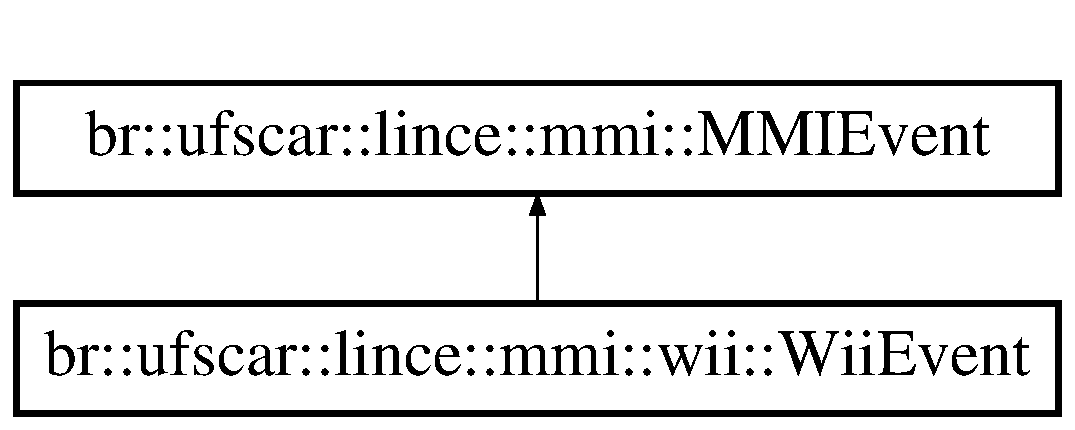
\includegraphics[height=2cm]{classbr_1_1ufscar_1_1lince_1_1mmi_1_1wii_1_1WiiEvent}
\end{center}
\end{figure}
\subsection*{Public Member Functions}
\begin{DoxyCompactItemize}
\item 
\hyperlink{classbr_1_1ufscar_1_1lince_1_1mmi_1_1wii_1_1WiiEvent_a19e75f8059636771751af5a60ecd3e32}{WiiEvent} (string \hyperlink{classbr_1_1ufscar_1_1lince_1_1mmi_1_1MMIEvent_ab49d18c433659ed8e7dbdaa9004839d5}{deviceId}, \hyperlink{namespacebr_1_1ufscar_1_1lince_1_1mmi_1_1wii_ac3b3ecd83aff16881b7c4749768d6145}{MoveAction} moveType)
\begin{DoxyCompactList}\small\item\em Construtor. \item\end{DoxyCompactList}\item 
virtual \hyperlink{classbr_1_1ufscar_1_1lince_1_1mmi_1_1wii_1_1WiiEvent_ace3a3623e886671767522e4c7d28e2bb}{$\sim$WiiEvent} ()
\begin{DoxyCompactList}\small\item\em Destructor. \item\end{DoxyCompactList}\item 
\hyperlink{namespacebr_1_1ufscar_1_1lince_1_1mmi_1_1wii_ac3b3ecd83aff16881b7c4749768d6145}{MoveAction} \hyperlink{classbr_1_1ufscar_1_1lince_1_1mmi_1_1wii_1_1WiiEvent_a1bd7fdbcc56be18c294108041f8d65ee}{getMoveAction} ()
\begin{DoxyCompactList}\small\item\em This methods returns the movement associate with the \hyperlink{classbr_1_1ufscar_1_1lince_1_1mmi_1_1wii_1_1WiiEvent}{WiiEvent}. \item\end{DoxyCompactList}\end{DoxyCompactItemize}


\subsection{Detailed Description}
This class represents a interaction realized with the \hyperlink{classbr_1_1ufscar_1_1lince_1_1mmi_1_1wii_1_1WiiMote}{WiiMote}. 

\subsection{Constructor \& Destructor Documentation}
\hypertarget{classbr_1_1ufscar_1_1lince_1_1mmi_1_1wii_1_1WiiEvent_a19e75f8059636771751af5a60ecd3e32}{
\index{br::ufscar::lince::mmi::wii::WiiEvent@{br::ufscar::lince::mmi::wii::WiiEvent}!WiiEvent@{WiiEvent}}
\index{WiiEvent@{WiiEvent}!br::ufscar::lince::mmi::wii::WiiEvent@{br::ufscar::lince::mmi::wii::WiiEvent}}
\subsubsection[{WiiEvent}]{\setlength{\rightskip}{0pt plus 5cm}br::ufscar::lince::mmi::wii::WiiEvent::WiiEvent (string {\em deviceId}, \/  {\bf MoveAction} {\em moveType})}}
\label{classbr_1_1ufscar_1_1lince_1_1mmi_1_1wii_1_1WiiEvent_a19e75f8059636771751af5a60ecd3e32}


Construtor. 


\begin{DoxyParams}{Parameters}
\item[{\em deviceId}]The id of the \hyperlink{classbr_1_1ufscar_1_1lince_1_1mmi_1_1wii_1_1WiiMote}{WiiMote} that generate the event \item[{\em moveType}]A representation of the movement recognized by the \hyperlink{classbr_1_1ufscar_1_1lince_1_1mmi_1_1wii_1_1WiiDriver}{WiiDriver}, \end{DoxyParams}
\hypertarget{classbr_1_1ufscar_1_1lince_1_1mmi_1_1wii_1_1WiiEvent_ace3a3623e886671767522e4c7d28e2bb}{
\index{br::ufscar::lince::mmi::wii::WiiEvent@{br::ufscar::lince::mmi::wii::WiiEvent}!$\sim$WiiEvent@{$\sim$WiiEvent}}
\index{$\sim$WiiEvent@{$\sim$WiiEvent}!br::ufscar::lince::mmi::wii::WiiEvent@{br::ufscar::lince::mmi::wii::WiiEvent}}
\subsubsection[{$\sim$WiiEvent}]{\setlength{\rightskip}{0pt plus 5cm}virtual br::ufscar::lince::mmi::wii::WiiEvent::$\sim$WiiEvent ()\hspace{0.3cm}{\ttfamily  \mbox{[}virtual\mbox{]}}}}
\label{classbr_1_1ufscar_1_1lince_1_1mmi_1_1wii_1_1WiiEvent_ace3a3623e886671767522e4c7d28e2bb}


Destructor. 



\subsection{Member Function Documentation}
\hypertarget{classbr_1_1ufscar_1_1lince_1_1mmi_1_1wii_1_1WiiEvent_a1bd7fdbcc56be18c294108041f8d65ee}{
\index{br::ufscar::lince::mmi::wii::WiiEvent@{br::ufscar::lince::mmi::wii::WiiEvent}!getMoveAction@{getMoveAction}}
\index{getMoveAction@{getMoveAction}!br::ufscar::lince::mmi::wii::WiiEvent@{br::ufscar::lince::mmi::wii::WiiEvent}}
\subsubsection[{getMoveAction}]{\setlength{\rightskip}{0pt plus 5cm}{\bf MoveAction} br::ufscar::lince::mmi::wii::WiiEvent::getMoveAction ()}}
\label{classbr_1_1ufscar_1_1lince_1_1mmi_1_1wii_1_1WiiEvent_a1bd7fdbcc56be18c294108041f8d65ee}


This methods returns the movement associate with the \hyperlink{classbr_1_1ufscar_1_1lince_1_1mmi_1_1wii_1_1WiiEvent}{WiiEvent}. 

\begin{DoxyReturn}{Returns}
A representation of the movement associate with the \hyperlink{classbr_1_1ufscar_1_1lince_1_1mmi_1_1wii_1_1WiiEvent}{WiiEvent} instance. 
\end{DoxyReturn}


The documentation for this class was generated from the following file:\begin{DoxyCompactItemize}
\item 
include/wii/\hyperlink{WiiEvent_8h}{WiiEvent.h}\end{DoxyCompactItemize}

\hypertarget{classbr_1_1ufscar_1_1lince_1_1mmi_1_1wii_1_1WiiEventHandler}{
\section{br::ufscar::lince::mmi::wii::WiiEventHandler Class Reference}
\label{classbr_1_1ufscar_1_1lince_1_1mmi_1_1wii_1_1WiiEventHandler}\index{br::ufscar::lince::mmi::wii::WiiEventHandler@{br::ufscar::lince::mmi::wii::WiiEventHandler}}
}


{\ttfamily \#include $<$WiiEventHandler.h$>$}

Inheritance diagram for br::ufscar::lince::mmi::wii::WiiEventHandler:\begin{figure}[H]
\begin{center}
\leavevmode
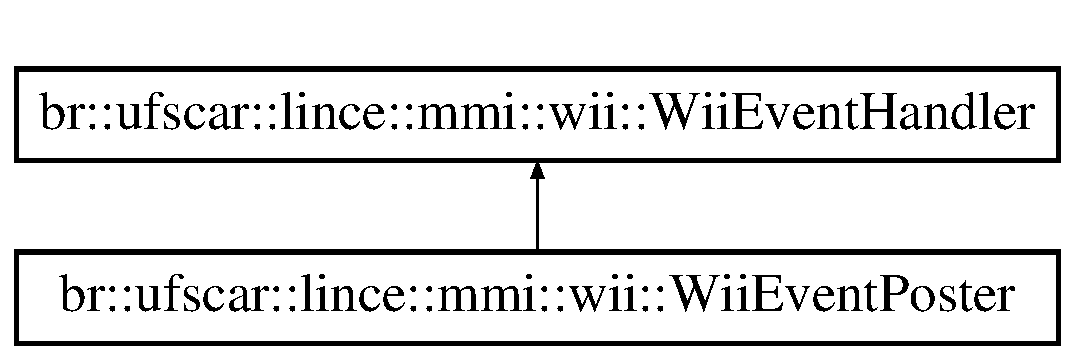
\includegraphics[height=2cm]{classbr_1_1ufscar_1_1lince_1_1mmi_1_1wii_1_1WiiEventHandler}
\end{center}
\end{figure}
\subsection*{Public Member Functions}
\begin{DoxyCompactItemize}
\item 
virtual void \hyperlink{classbr_1_1ufscar_1_1lince_1_1mmi_1_1wii_1_1WiiEventHandler_a7e94bf7dc7fa2dd0552ff2c97faf9f41}{sendEvent} (\hyperlink{classbr_1_1ufscar_1_1lince_1_1mmi_1_1MMIEvent}{MMIEvent} $\ast$event)=0
\item 
virtual \hyperlink{classbr_1_1ufscar_1_1lince_1_1mmi_1_1wii_1_1WiiEventHandler_ab2407ecc0060c55e9b89241c3abc4eb4}{$\sim$WiiEventHandler} ()
\end{DoxyCompactItemize}


\subsection{Constructor \& Destructor Documentation}
\hypertarget{classbr_1_1ufscar_1_1lince_1_1mmi_1_1wii_1_1WiiEventHandler_ab2407ecc0060c55e9b89241c3abc4eb4}{
\index{br::ufscar::lince::mmi::wii::WiiEventHandler@{br::ufscar::lince::mmi::wii::WiiEventHandler}!$\sim$WiiEventHandler@{$\sim$WiiEventHandler}}
\index{$\sim$WiiEventHandler@{$\sim$WiiEventHandler}!br::ufscar::lince::mmi::wii::WiiEventHandler@{br::ufscar::lince::mmi::wii::WiiEventHandler}}
\subsubsection[{$\sim$WiiEventHandler}]{\setlength{\rightskip}{0pt plus 5cm}virtual br::ufscar::lince::mmi::wii::WiiEventHandler::$\sim$WiiEventHandler ()\hspace{0.3cm}{\ttfamily  \mbox{[}inline, virtual\mbox{]}}}}
\label{classbr_1_1ufscar_1_1lince_1_1mmi_1_1wii_1_1WiiEventHandler_ab2407ecc0060c55e9b89241c3abc4eb4}


\subsection{Member Function Documentation}
\hypertarget{classbr_1_1ufscar_1_1lince_1_1mmi_1_1wii_1_1WiiEventHandler_a7e94bf7dc7fa2dd0552ff2c97faf9f41}{
\index{br::ufscar::lince::mmi::wii::WiiEventHandler@{br::ufscar::lince::mmi::wii::WiiEventHandler}!sendEvent@{sendEvent}}
\index{sendEvent@{sendEvent}!br::ufscar::lince::mmi::wii::WiiEventHandler@{br::ufscar::lince::mmi::wii::WiiEventHandler}}
\subsubsection[{sendEvent}]{\setlength{\rightskip}{0pt plus 5cm}virtual void br::ufscar::lince::mmi::wii::WiiEventHandler::sendEvent ({\bf MMIEvent} $\ast$ {\em event})\hspace{0.3cm}{\ttfamily  \mbox{[}pure virtual\mbox{]}}}}
\label{classbr_1_1ufscar_1_1lince_1_1mmi_1_1wii_1_1WiiEventHandler_a7e94bf7dc7fa2dd0552ff2c97faf9f41}


Implemented in \hyperlink{classbr_1_1ufscar_1_1lince_1_1mmi_1_1wii_1_1WiiEventPoster_a5e1eb67b8afb4324be1899a043ee92c4}{br::ufscar::lince::mmi::wii::WiiEventPoster}.



The documentation for this class was generated from the following file:\begin{DoxyCompactItemize}
\item 
include/wii/\hyperlink{WiiEventHandler_8h}{WiiEventHandler.h}\end{DoxyCompactItemize}

\hypertarget{classbr_1_1ufscar_1_1lince_1_1mmi_1_1wii_1_1WiiEventPoster}{
\section{br::ufscar::lince::mmi::wii::WiiEventPoster Class Reference}
\label{classbr_1_1ufscar_1_1lince_1_1mmi_1_1wii_1_1WiiEventPoster}\index{br::ufscar::lince::mmi::wii::WiiEventPoster@{br::ufscar::lince::mmi::wii::WiiEventPoster}}
}


{\ttfamily \#include $<$WiiEventPoster.h$>$}

Inheritance diagram for br::ufscar::lince::mmi::wii::WiiEventPoster:\begin{figure}[H]
\begin{center}
\leavevmode
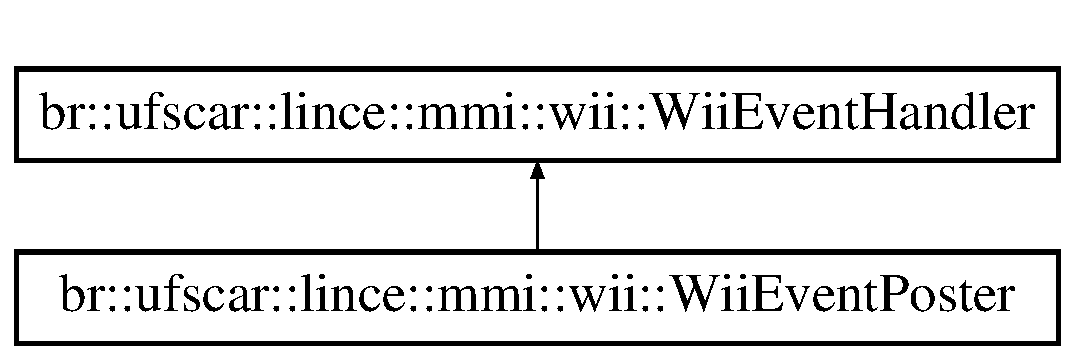
\includegraphics[height=2cm]{classbr_1_1ufscar_1_1lince_1_1mmi_1_1wii_1_1WiiEventPoster}
\end{center}
\end{figure}
\subsection*{Public Member Functions}
\begin{DoxyCompactItemize}
\item 
\hyperlink{classbr_1_1ufscar_1_1lince_1_1mmi_1_1wii_1_1WiiEventPoster_a36425c0fcb515ff86f97cb68b2bd70e7}{WiiEventPoster} ()
\item 
virtual \hyperlink{classbr_1_1ufscar_1_1lince_1_1mmi_1_1wii_1_1WiiEventPoster_aef8a15c7fc7e8d3b02673cd08e799fd1}{$\sim$WiiEventPoster} ()
\item 
void \hyperlink{classbr_1_1ufscar_1_1lince_1_1mmi_1_1wii_1_1WiiEventPoster_a5e1eb67b8afb4324be1899a043ee92c4}{sendEvent} (\hyperlink{classbr_1_1ufscar_1_1lince_1_1mmi_1_1MMIEvent}{MMIEvent} $\ast$event)
\end{DoxyCompactItemize}


\subsection{Constructor \& Destructor Documentation}
\hypertarget{classbr_1_1ufscar_1_1lince_1_1mmi_1_1wii_1_1WiiEventPoster_a36425c0fcb515ff86f97cb68b2bd70e7}{
\index{br::ufscar::lince::mmi::wii::WiiEventPoster@{br::ufscar::lince::mmi::wii::WiiEventPoster}!WiiEventPoster@{WiiEventPoster}}
\index{WiiEventPoster@{WiiEventPoster}!br::ufscar::lince::mmi::wii::WiiEventPoster@{br::ufscar::lince::mmi::wii::WiiEventPoster}}
\subsubsection[{WiiEventPoster}]{\setlength{\rightskip}{0pt plus 5cm}br::ufscar::lince::mmi::wii::WiiEventPoster::WiiEventPoster ()}}
\label{classbr_1_1ufscar_1_1lince_1_1mmi_1_1wii_1_1WiiEventPoster_a36425c0fcb515ff86f97cb68b2bd70e7}
\hypertarget{classbr_1_1ufscar_1_1lince_1_1mmi_1_1wii_1_1WiiEventPoster_aef8a15c7fc7e8d3b02673cd08e799fd1}{
\index{br::ufscar::lince::mmi::wii::WiiEventPoster@{br::ufscar::lince::mmi::wii::WiiEventPoster}!$\sim$WiiEventPoster@{$\sim$WiiEventPoster}}
\index{$\sim$WiiEventPoster@{$\sim$WiiEventPoster}!br::ufscar::lince::mmi::wii::WiiEventPoster@{br::ufscar::lince::mmi::wii::WiiEventPoster}}
\subsubsection[{$\sim$WiiEventPoster}]{\setlength{\rightskip}{0pt plus 5cm}virtual br::ufscar::lince::mmi::wii::WiiEventPoster::$\sim$WiiEventPoster ()\hspace{0.3cm}{\ttfamily  \mbox{[}virtual\mbox{]}}}}
\label{classbr_1_1ufscar_1_1lince_1_1mmi_1_1wii_1_1WiiEventPoster_aef8a15c7fc7e8d3b02673cd08e799fd1}


\subsection{Member Function Documentation}
\hypertarget{classbr_1_1ufscar_1_1lince_1_1mmi_1_1wii_1_1WiiEventPoster_a5e1eb67b8afb4324be1899a043ee92c4}{
\index{br::ufscar::lince::mmi::wii::WiiEventPoster@{br::ufscar::lince::mmi::wii::WiiEventPoster}!sendEvent@{sendEvent}}
\index{sendEvent@{sendEvent}!br::ufscar::lince::mmi::wii::WiiEventPoster@{br::ufscar::lince::mmi::wii::WiiEventPoster}}
\subsubsection[{sendEvent}]{\setlength{\rightskip}{0pt plus 5cm}void br::ufscar::lince::mmi::wii::WiiEventPoster::sendEvent ({\bf MMIEvent} $\ast$ {\em event})\hspace{0.3cm}{\ttfamily  \mbox{[}virtual\mbox{]}}}}
\label{classbr_1_1ufscar_1_1lince_1_1mmi_1_1wii_1_1WiiEventPoster_a5e1eb67b8afb4324be1899a043ee92c4}


Implements \hyperlink{classbr_1_1ufscar_1_1lince_1_1mmi_1_1wii_1_1WiiEventHandler_a7e94bf7dc7fa2dd0552ff2c97faf9f41}{br::ufscar::lince::mmi::wii::WiiEventHandler}.



The documentation for this class was generated from the following file:\begin{DoxyCompactItemize}
\item 
include/wii/\hyperlink{WiiEventPoster_8h}{WiiEventPoster.h}\end{DoxyCompactItemize}

\hypertarget{classbr_1_1ufscar_1_1lince_1_1mmi_1_1wii_1_1WiiMote}{
\section{br::ufscar::lince::mmi::wii::WiiMote Class Reference}
\label{classbr_1_1ufscar_1_1lince_1_1mmi_1_1wii_1_1WiiMote}\index{br::ufscar::lince::mmi::wii::WiiMote@{br::ufscar::lince::mmi::wii::WiiMote}}
}


{\ttfamily \#include $<$WiiMote.h$>$}

Inheritance diagram for br::ufscar::lince::mmi::wii::WiiMote:\begin{figure}[H]
\begin{center}
\leavevmode
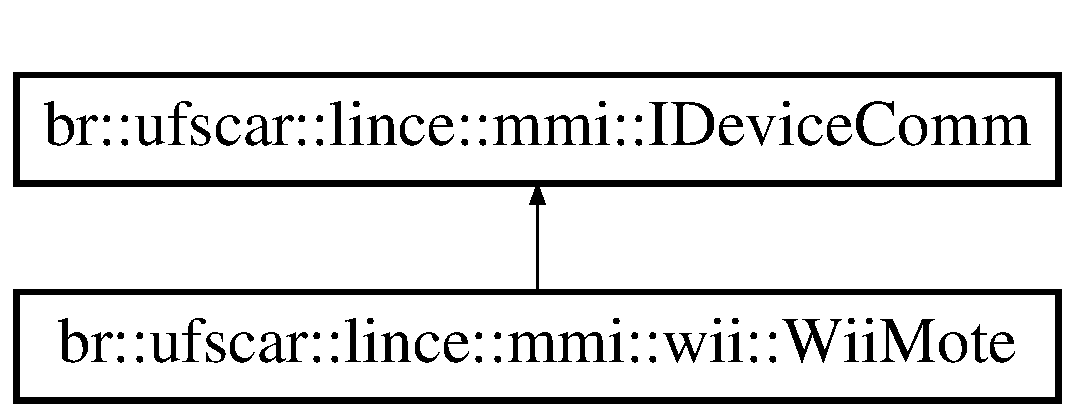
\includegraphics[height=2cm]{classbr_1_1ufscar_1_1lince_1_1mmi_1_1wii_1_1WiiMote}
\end{center}
\end{figure}
\subsection*{Public Member Functions}
\begin{DoxyCompactItemize}
\item 
\hyperlink{classbr_1_1ufscar_1_1lince_1_1mmi_1_1wii_1_1WiiMote_a286176220d743bd02ee02b35970916a3}{WiiMote} (\hyperlink{classbr_1_1ufscar_1_1lince_1_1mmi_1_1wii_1_1WiiEventHandler}{WiiEventHandler} $\ast$handler, unsigned char reportEvents=\hyperlink{classbr_1_1ufscar_1_1lince_1_1mmi_1_1wii_1_1WiiMote_a96872905a37ca4eb5902ea220217a54f}{REPORT\_\-ALL})
\item 
virtual \hyperlink{classbr_1_1ufscar_1_1lince_1_1mmi_1_1wii_1_1WiiMote_aa0a674eed3f5c4cebf761682dbcdf6e8}{$\sim$WiiMote} ()
\item 
virtual void \hyperlink{classbr_1_1ufscar_1_1lince_1_1mmi_1_1wii_1_1WiiMote_a15e0d1b2ac9fde887e870aeb597c0dc8}{connect} ()
\begin{DoxyCompactList}\small\item\em This method stabilishes a connect between the device and the \hyperlink{classbr_1_1ufscar_1_1lince_1_1mmi_1_1MMIManager}{MMIManager}, allowing the device reports his multimodal events. \item\end{DoxyCompactList}\item 
virtual void \hyperlink{classbr_1_1ufscar_1_1lince_1_1mmi_1_1wii_1_1WiiMote_a44aa8cf98660392a91045e4892a9e65a}{disconnect} ()
\begin{DoxyCompactList}\small\item\em This method finishes the connection between the devica and \hyperlink{classbr_1_1ufscar_1_1lince_1_1mmi_1_1MMIManager}{MMIManager}. \item\end{DoxyCompactList}\item 
virtual void \hyperlink{classbr_1_1ufscar_1_1lince_1_1mmi_1_1wii_1_1WiiMote_acd1fe851dd5909ee3cbd0fa23a070f0e}{sendToDevice} (vector$<$ string $>$ $\ast$args)
\begin{DoxyCompactList}\small\item\em This method allows send a message to the device. \item\end{DoxyCompactList}\item 
virtual string \hyperlink{classbr_1_1ufscar_1_1lince_1_1mmi_1_1wii_1_1WiiMote_a125dc3805711f4b5fa9327ebf719e035}{getDeviceId} ()
\begin{DoxyCompactList}\small\item\em This method return the id of the device. \item\end{DoxyCompactList}\item 
virtual void \hyperlink{classbr_1_1ufscar_1_1lince_1_1mmi_1_1wii_1_1WiiMote_a4d17da2514583aa3787a1d9fda1cd74c}{release} ()
\begin{DoxyCompactList}\small\item\em This method make the device reset its internals variables. \item\end{DoxyCompactList}\item 
bool \hyperlink{classbr_1_1ufscar_1_1lince_1_1mmi_1_1wii_1_1WiiMote_aa3b9e2935b6f0fc39b1a08260f3da66d}{isReportingButtons} ()
\item 
bool \hyperlink{classbr_1_1ufscar_1_1lince_1_1mmi_1_1wii_1_1WiiMote_a969959e1b25dd2660e54d1e3acd520a4}{isReportingAcceleration} ()
\item 
bool \hyperlink{classbr_1_1ufscar_1_1lince_1_1mmi_1_1wii_1_1WiiMote_a1eeed1b89ee5cd55fedf9f8c75561ed0}{isReportingMoves} ()
\end{DoxyCompactItemize}
\subsection*{Static Public Attributes}
\begin{DoxyCompactItemize}
\item 
static const unsigned char \hyperlink{classbr_1_1ufscar_1_1lince_1_1mmi_1_1wii_1_1WiiMote_af1e2bc7d7054d1b4dab67e9b278017ce}{REPORT\_\-BUTTONS}
\item 
static const unsigned char \hyperlink{classbr_1_1ufscar_1_1lince_1_1mmi_1_1wii_1_1WiiMote_a31e84ef1eebb0340545dcd1b3bb3a0fc}{REPORT\_\-ACCELERATION}
\item 
static const unsigned char \hyperlink{classbr_1_1ufscar_1_1lince_1_1mmi_1_1wii_1_1WiiMote_a95ac41c7b1b12e770e2adf6f12f48143}{REPORT\_\-MOVES}
\item 
static const unsigned char \hyperlink{classbr_1_1ufscar_1_1lince_1_1mmi_1_1wii_1_1WiiMote_a96872905a37ca4eb5902ea220217a54f}{REPORT\_\-ALL}
\end{DoxyCompactItemize}
\subsection*{Protected Member Functions}
\begin{DoxyCompactItemize}
\item 
int \hyperlink{classbr_1_1ufscar_1_1lince_1_1mmi_1_1wii_1_1WiiMote_aafcb4ce9fbe1af60e2dcc3a4baca239e}{evalueMassCenterAccX} ()
\item 
int \hyperlink{classbr_1_1ufscar_1_1lince_1_1mmi_1_1wii_1_1WiiMote_aa6b36913433189b48dc26595bb0f91dc}{evalueMassCenterAccY} ()
\item 
int \hyperlink{classbr_1_1ufscar_1_1lince_1_1mmi_1_1wii_1_1WiiMote_a0c49aa47a11e98f20fa720603a20c14f}{evalueMassCenterAccZ} ()
\item 
virtual void \hyperlink{classbr_1_1ufscar_1_1lince_1_1mmi_1_1wii_1_1WiiMote_ae0f3e542c2d18e7a09c2beb09562a7d4}{run} ()
\end{DoxyCompactItemize}


\subsection{Constructor \& Destructor Documentation}
\hypertarget{classbr_1_1ufscar_1_1lince_1_1mmi_1_1wii_1_1WiiMote_a286176220d743bd02ee02b35970916a3}{
\index{br::ufscar::lince::mmi::wii::WiiMote@{br::ufscar::lince::mmi::wii::WiiMote}!WiiMote@{WiiMote}}
\index{WiiMote@{WiiMote}!br::ufscar::lince::mmi::wii::WiiMote@{br::ufscar::lince::mmi::wii::WiiMote}}
\subsubsection[{WiiMote}]{\setlength{\rightskip}{0pt plus 5cm}br::ufscar::lince::mmi::wii::WiiMote::WiiMote ({\bf WiiEventHandler} $\ast$ {\em handler}, \/  unsigned char {\em reportEvents} = {\ttfamily {\bf REPORT\_\-ALL}})}}
\label{classbr_1_1ufscar_1_1lince_1_1mmi_1_1wii_1_1WiiMote_a286176220d743bd02ee02b35970916a3}
\hypertarget{classbr_1_1ufscar_1_1lince_1_1mmi_1_1wii_1_1WiiMote_aa0a674eed3f5c4cebf761682dbcdf6e8}{
\index{br::ufscar::lince::mmi::wii::WiiMote@{br::ufscar::lince::mmi::wii::WiiMote}!$\sim$WiiMote@{$\sim$WiiMote}}
\index{$\sim$WiiMote@{$\sim$WiiMote}!br::ufscar::lince::mmi::wii::WiiMote@{br::ufscar::lince::mmi::wii::WiiMote}}
\subsubsection[{$\sim$WiiMote}]{\setlength{\rightskip}{0pt plus 5cm}virtual br::ufscar::lince::mmi::wii::WiiMote::$\sim$WiiMote ()\hspace{0.3cm}{\ttfamily  \mbox{[}virtual\mbox{]}}}}
\label{classbr_1_1ufscar_1_1lince_1_1mmi_1_1wii_1_1WiiMote_aa0a674eed3f5c4cebf761682dbcdf6e8}


\subsection{Member Function Documentation}
\hypertarget{classbr_1_1ufscar_1_1lince_1_1mmi_1_1wii_1_1WiiMote_a15e0d1b2ac9fde887e870aeb597c0dc8}{
\index{br::ufscar::lince::mmi::wii::WiiMote@{br::ufscar::lince::mmi::wii::WiiMote}!connect@{connect}}
\index{connect@{connect}!br::ufscar::lince::mmi::wii::WiiMote@{br::ufscar::lince::mmi::wii::WiiMote}}
\subsubsection[{connect}]{\setlength{\rightskip}{0pt plus 5cm}virtual void br::ufscar::lince::mmi::wii::WiiMote::connect ()\hspace{0.3cm}{\ttfamily  \mbox{[}virtual\mbox{]}}}}
\label{classbr_1_1ufscar_1_1lince_1_1mmi_1_1wii_1_1WiiMote_a15e0d1b2ac9fde887e870aeb597c0dc8}


This method stabilishes a connect between the device and the \hyperlink{classbr_1_1ufscar_1_1lince_1_1mmi_1_1MMIManager}{MMIManager}, allowing the device reports his multimodal events. 



Implements \hyperlink{classbr_1_1ufscar_1_1lince_1_1mmi_1_1IDeviceComm_a53f48993f294b9a755125b6ccdb06ad4}{br::ufscar::lince::mmi::IDeviceComm}.

\hypertarget{classbr_1_1ufscar_1_1lince_1_1mmi_1_1wii_1_1WiiMote_a44aa8cf98660392a91045e4892a9e65a}{
\index{br::ufscar::lince::mmi::wii::WiiMote@{br::ufscar::lince::mmi::wii::WiiMote}!disconnect@{disconnect}}
\index{disconnect@{disconnect}!br::ufscar::lince::mmi::wii::WiiMote@{br::ufscar::lince::mmi::wii::WiiMote}}
\subsubsection[{disconnect}]{\setlength{\rightskip}{0pt plus 5cm}virtual void br::ufscar::lince::mmi::wii::WiiMote::disconnect ()\hspace{0.3cm}{\ttfamily  \mbox{[}virtual\mbox{]}}}}
\label{classbr_1_1ufscar_1_1lince_1_1mmi_1_1wii_1_1WiiMote_a44aa8cf98660392a91045e4892a9e65a}


This method finishes the connection between the devica and \hyperlink{classbr_1_1ufscar_1_1lince_1_1mmi_1_1MMIManager}{MMIManager}. 



Implements \hyperlink{classbr_1_1ufscar_1_1lince_1_1mmi_1_1IDeviceComm_ad3791cf1ab234f4a6b464c3f614c78c6}{br::ufscar::lince::mmi::IDeviceComm}.

\hypertarget{classbr_1_1ufscar_1_1lince_1_1mmi_1_1wii_1_1WiiMote_aafcb4ce9fbe1af60e2dcc3a4baca239e}{
\index{br::ufscar::lince::mmi::wii::WiiMote@{br::ufscar::lince::mmi::wii::WiiMote}!evalueMassCenterAccX@{evalueMassCenterAccX}}
\index{evalueMassCenterAccX@{evalueMassCenterAccX}!br::ufscar::lince::mmi::wii::WiiMote@{br::ufscar::lince::mmi::wii::WiiMote}}
\subsubsection[{evalueMassCenterAccX}]{\setlength{\rightskip}{0pt plus 5cm}int br::ufscar::lince::mmi::wii::WiiMote::evalueMassCenterAccX ()\hspace{0.3cm}{\ttfamily  \mbox{[}protected\mbox{]}}}}
\label{classbr_1_1ufscar_1_1lince_1_1mmi_1_1wii_1_1WiiMote_aafcb4ce9fbe1af60e2dcc3a4baca239e}
\hypertarget{classbr_1_1ufscar_1_1lince_1_1mmi_1_1wii_1_1WiiMote_aa6b36913433189b48dc26595bb0f91dc}{
\index{br::ufscar::lince::mmi::wii::WiiMote@{br::ufscar::lince::mmi::wii::WiiMote}!evalueMassCenterAccY@{evalueMassCenterAccY}}
\index{evalueMassCenterAccY@{evalueMassCenterAccY}!br::ufscar::lince::mmi::wii::WiiMote@{br::ufscar::lince::mmi::wii::WiiMote}}
\subsubsection[{evalueMassCenterAccY}]{\setlength{\rightskip}{0pt plus 5cm}int br::ufscar::lince::mmi::wii::WiiMote::evalueMassCenterAccY ()\hspace{0.3cm}{\ttfamily  \mbox{[}protected\mbox{]}}}}
\label{classbr_1_1ufscar_1_1lince_1_1mmi_1_1wii_1_1WiiMote_aa6b36913433189b48dc26595bb0f91dc}
\hypertarget{classbr_1_1ufscar_1_1lince_1_1mmi_1_1wii_1_1WiiMote_a0c49aa47a11e98f20fa720603a20c14f}{
\index{br::ufscar::lince::mmi::wii::WiiMote@{br::ufscar::lince::mmi::wii::WiiMote}!evalueMassCenterAccZ@{evalueMassCenterAccZ}}
\index{evalueMassCenterAccZ@{evalueMassCenterAccZ}!br::ufscar::lince::mmi::wii::WiiMote@{br::ufscar::lince::mmi::wii::WiiMote}}
\subsubsection[{evalueMassCenterAccZ}]{\setlength{\rightskip}{0pt plus 5cm}int br::ufscar::lince::mmi::wii::WiiMote::evalueMassCenterAccZ ()\hspace{0.3cm}{\ttfamily  \mbox{[}protected\mbox{]}}}}
\label{classbr_1_1ufscar_1_1lince_1_1mmi_1_1wii_1_1WiiMote_a0c49aa47a11e98f20fa720603a20c14f}
\hypertarget{classbr_1_1ufscar_1_1lince_1_1mmi_1_1wii_1_1WiiMote_a125dc3805711f4b5fa9327ebf719e035}{
\index{br::ufscar::lince::mmi::wii::WiiMote@{br::ufscar::lince::mmi::wii::WiiMote}!getDeviceId@{getDeviceId}}
\index{getDeviceId@{getDeviceId}!br::ufscar::lince::mmi::wii::WiiMote@{br::ufscar::lince::mmi::wii::WiiMote}}
\subsubsection[{getDeviceId}]{\setlength{\rightskip}{0pt plus 5cm}virtual string br::ufscar::lince::mmi::wii::WiiMote::getDeviceId ()\hspace{0.3cm}{\ttfamily  \mbox{[}virtual\mbox{]}}}}
\label{classbr_1_1ufscar_1_1lince_1_1mmi_1_1wii_1_1WiiMote_a125dc3805711f4b5fa9327ebf719e035}


This method return the id of the device. 

\begin{DoxyReturn}{Returns}
Device identification. 
\end{DoxyReturn}


Implements \hyperlink{classbr_1_1ufscar_1_1lince_1_1mmi_1_1IDeviceComm_a4ae69c19445713ddc9fda351555c1ac2}{br::ufscar::lince::mmi::IDeviceComm}.

\hypertarget{classbr_1_1ufscar_1_1lince_1_1mmi_1_1wii_1_1WiiMote_a969959e1b25dd2660e54d1e3acd520a4}{
\index{br::ufscar::lince::mmi::wii::WiiMote@{br::ufscar::lince::mmi::wii::WiiMote}!isReportingAcceleration@{isReportingAcceleration}}
\index{isReportingAcceleration@{isReportingAcceleration}!br::ufscar::lince::mmi::wii::WiiMote@{br::ufscar::lince::mmi::wii::WiiMote}}
\subsubsection[{isReportingAcceleration}]{\setlength{\rightskip}{0pt plus 5cm}bool br::ufscar::lince::mmi::wii::WiiMote::isReportingAcceleration ()\hspace{0.3cm}{\ttfamily  \mbox{[}inline\mbox{]}}}}
\label{classbr_1_1ufscar_1_1lince_1_1mmi_1_1wii_1_1WiiMote_a969959e1b25dd2660e54d1e3acd520a4}
\hypertarget{classbr_1_1ufscar_1_1lince_1_1mmi_1_1wii_1_1WiiMote_aa3b9e2935b6f0fc39b1a08260f3da66d}{
\index{br::ufscar::lince::mmi::wii::WiiMote@{br::ufscar::lince::mmi::wii::WiiMote}!isReportingButtons@{isReportingButtons}}
\index{isReportingButtons@{isReportingButtons}!br::ufscar::lince::mmi::wii::WiiMote@{br::ufscar::lince::mmi::wii::WiiMote}}
\subsubsection[{isReportingButtons}]{\setlength{\rightskip}{0pt plus 5cm}bool br::ufscar::lince::mmi::wii::WiiMote::isReportingButtons ()\hspace{0.3cm}{\ttfamily  \mbox{[}inline\mbox{]}}}}
\label{classbr_1_1ufscar_1_1lince_1_1mmi_1_1wii_1_1WiiMote_aa3b9e2935b6f0fc39b1a08260f3da66d}
\hypertarget{classbr_1_1ufscar_1_1lince_1_1mmi_1_1wii_1_1WiiMote_a1eeed1b89ee5cd55fedf9f8c75561ed0}{
\index{br::ufscar::lince::mmi::wii::WiiMote@{br::ufscar::lince::mmi::wii::WiiMote}!isReportingMoves@{isReportingMoves}}
\index{isReportingMoves@{isReportingMoves}!br::ufscar::lince::mmi::wii::WiiMote@{br::ufscar::lince::mmi::wii::WiiMote}}
\subsubsection[{isReportingMoves}]{\setlength{\rightskip}{0pt plus 5cm}bool br::ufscar::lince::mmi::wii::WiiMote::isReportingMoves ()\hspace{0.3cm}{\ttfamily  \mbox{[}inline\mbox{]}}}}
\label{classbr_1_1ufscar_1_1lince_1_1mmi_1_1wii_1_1WiiMote_a1eeed1b89ee5cd55fedf9f8c75561ed0}
\hypertarget{classbr_1_1ufscar_1_1lince_1_1mmi_1_1wii_1_1WiiMote_a4d17da2514583aa3787a1d9fda1cd74c}{
\index{br::ufscar::lince::mmi::wii::WiiMote@{br::ufscar::lince::mmi::wii::WiiMote}!release@{release}}
\index{release@{release}!br::ufscar::lince::mmi::wii::WiiMote@{br::ufscar::lince::mmi::wii::WiiMote}}
\subsubsection[{release}]{\setlength{\rightskip}{0pt plus 5cm}virtual void br::ufscar::lince::mmi::wii::WiiMote::release ()\hspace{0.3cm}{\ttfamily  \mbox{[}virtual\mbox{]}}}}
\label{classbr_1_1ufscar_1_1lince_1_1mmi_1_1wii_1_1WiiMote_a4d17da2514583aa3787a1d9fda1cd74c}


This method make the device reset its internals variables. 



Implements \hyperlink{classbr_1_1ufscar_1_1lince_1_1mmi_1_1IDeviceComm_a9c173ebb83a502e78143a52fc7d87a80}{br::ufscar::lince::mmi::IDeviceComm}.

\hypertarget{classbr_1_1ufscar_1_1lince_1_1mmi_1_1wii_1_1WiiMote_ae0f3e542c2d18e7a09c2beb09562a7d4}{
\index{br::ufscar::lince::mmi::wii::WiiMote@{br::ufscar::lince::mmi::wii::WiiMote}!run@{run}}
\index{run@{run}!br::ufscar::lince::mmi::wii::WiiMote@{br::ufscar::lince::mmi::wii::WiiMote}}
\subsubsection[{run}]{\setlength{\rightskip}{0pt plus 5cm}virtual void br::ufscar::lince::mmi::wii::WiiMote::run ()\hspace{0.3cm}{\ttfamily  \mbox{[}protected, virtual\mbox{]}}}}
\label{classbr_1_1ufscar_1_1lince_1_1mmi_1_1wii_1_1WiiMote_ae0f3e542c2d18e7a09c2beb09562a7d4}
\hypertarget{classbr_1_1ufscar_1_1lince_1_1mmi_1_1wii_1_1WiiMote_acd1fe851dd5909ee3cbd0fa23a070f0e}{
\index{br::ufscar::lince::mmi::wii::WiiMote@{br::ufscar::lince::mmi::wii::WiiMote}!sendToDevice@{sendToDevice}}
\index{sendToDevice@{sendToDevice}!br::ufscar::lince::mmi::wii::WiiMote@{br::ufscar::lince::mmi::wii::WiiMote}}
\subsubsection[{sendToDevice}]{\setlength{\rightskip}{0pt plus 5cm}virtual void br::ufscar::lince::mmi::wii::WiiMote::sendToDevice (vector$<$ string $>$ $\ast$ {\em args})\hspace{0.3cm}{\ttfamily  \mbox{[}virtual\mbox{]}}}}
\label{classbr_1_1ufscar_1_1lince_1_1mmi_1_1wii_1_1WiiMote_acd1fe851dd5909ee3cbd0fa23a070f0e}


This method allows send a message to the device. 


\begin{DoxyParams}{Parameters}
\item[{\em args}]A array of strings that will contain the message. \end{DoxyParams}


Implements \hyperlink{classbr_1_1ufscar_1_1lince_1_1mmi_1_1IDeviceComm_a0249a13030b4df9b50778723421375d9}{br::ufscar::lince::mmi::IDeviceComm}.



\subsection{Field Documentation}
\hypertarget{classbr_1_1ufscar_1_1lince_1_1mmi_1_1wii_1_1WiiMote_a31e84ef1eebb0340545dcd1b3bb3a0fc}{
\index{br::ufscar::lince::mmi::wii::WiiMote@{br::ufscar::lince::mmi::wii::WiiMote}!REPORT\_\-ACCELERATION@{REPORT\_\-ACCELERATION}}
\index{REPORT\_\-ACCELERATION@{REPORT\_\-ACCELERATION}!br::ufscar::lince::mmi::wii::WiiMote@{br::ufscar::lince::mmi::wii::WiiMote}}
\subsubsection[{REPORT\_\-ACCELERATION}]{\setlength{\rightskip}{0pt plus 5cm}const unsigned char {\bf br::ufscar::lince::mmi::wii::WiiMote::REPORT\_\-ACCELERATION}\hspace{0.3cm}{\ttfamily  \mbox{[}static\mbox{]}}}}
\label{classbr_1_1ufscar_1_1lince_1_1mmi_1_1wii_1_1WiiMote_a31e84ef1eebb0340545dcd1b3bb3a0fc}
\hypertarget{classbr_1_1ufscar_1_1lince_1_1mmi_1_1wii_1_1WiiMote_a96872905a37ca4eb5902ea220217a54f}{
\index{br::ufscar::lince::mmi::wii::WiiMote@{br::ufscar::lince::mmi::wii::WiiMote}!REPORT\_\-ALL@{REPORT\_\-ALL}}
\index{REPORT\_\-ALL@{REPORT\_\-ALL}!br::ufscar::lince::mmi::wii::WiiMote@{br::ufscar::lince::mmi::wii::WiiMote}}
\subsubsection[{REPORT\_\-ALL}]{\setlength{\rightskip}{0pt plus 5cm}const unsigned char {\bf br::ufscar::lince::mmi::wii::WiiMote::REPORT\_\-ALL}\hspace{0.3cm}{\ttfamily  \mbox{[}static\mbox{]}}}}
\label{classbr_1_1ufscar_1_1lince_1_1mmi_1_1wii_1_1WiiMote_a96872905a37ca4eb5902ea220217a54f}
\hypertarget{classbr_1_1ufscar_1_1lince_1_1mmi_1_1wii_1_1WiiMote_af1e2bc7d7054d1b4dab67e9b278017ce}{
\index{br::ufscar::lince::mmi::wii::WiiMote@{br::ufscar::lince::mmi::wii::WiiMote}!REPORT\_\-BUTTONS@{REPORT\_\-BUTTONS}}
\index{REPORT\_\-BUTTONS@{REPORT\_\-BUTTONS}!br::ufscar::lince::mmi::wii::WiiMote@{br::ufscar::lince::mmi::wii::WiiMote}}
\subsubsection[{REPORT\_\-BUTTONS}]{\setlength{\rightskip}{0pt plus 5cm}const unsigned char {\bf br::ufscar::lince::mmi::wii::WiiMote::REPORT\_\-BUTTONS}\hspace{0.3cm}{\ttfamily  \mbox{[}static\mbox{]}}}}
\label{classbr_1_1ufscar_1_1lince_1_1mmi_1_1wii_1_1WiiMote_af1e2bc7d7054d1b4dab67e9b278017ce}
\hypertarget{classbr_1_1ufscar_1_1lince_1_1mmi_1_1wii_1_1WiiMote_a95ac41c7b1b12e770e2adf6f12f48143}{
\index{br::ufscar::lince::mmi::wii::WiiMote@{br::ufscar::lince::mmi::wii::WiiMote}!REPORT\_\-MOVES@{REPORT\_\-MOVES}}
\index{REPORT\_\-MOVES@{REPORT\_\-MOVES}!br::ufscar::lince::mmi::wii::WiiMote@{br::ufscar::lince::mmi::wii::WiiMote}}
\subsubsection[{REPORT\_\-MOVES}]{\setlength{\rightskip}{0pt plus 5cm}const unsigned char {\bf br::ufscar::lince::mmi::wii::WiiMote::REPORT\_\-MOVES}\hspace{0.3cm}{\ttfamily  \mbox{[}static\mbox{]}}}}
\label{classbr_1_1ufscar_1_1lince_1_1mmi_1_1wii_1_1WiiMote_a95ac41c7b1b12e770e2adf6f12f48143}


The documentation for this class was generated from the following file:\begin{DoxyCompactItemize}
\item 
include/wii/\hyperlink{WiiMote_8h}{WiiMote.h}\end{DoxyCompactItemize}

\hypertarget{classbr_1_1ufscar_1_1lince_1_1mmi_1_1wii_1_1WiiState}{
\section{br::ufscar::lince::mmi::wii::WiiState Class Reference}
\label{classbr_1_1ufscar_1_1lince_1_1mmi_1_1wii_1_1WiiState}\index{br::ufscar::lince::mmi::wii::WiiState@{br::ufscar::lince::mmi::wii::WiiState}}
}


{\ttfamily \#include $<$WiiState.h$>$}

\subsection*{Public Member Functions}
\begin{DoxyCompactItemize}
\item 
\hyperlink{classbr_1_1ufscar_1_1lince_1_1mmi_1_1wii_1_1WiiState_a495f2533098a39cab292f4c090f586fc}{WiiState} (\hyperlink{classbr_1_1ufscar_1_1lince_1_1mmi_1_1wii_1_1WiiState}{WiiState} $\ast$copy)
\item 
\hyperlink{classbr_1_1ufscar_1_1lince_1_1mmi_1_1wii_1_1WiiState_a3dcbaf91a80e3638a097c09078776ba0}{WiiState} (cwiid\_\-state nState)
\item 
\hyperlink{classbr_1_1ufscar_1_1lince_1_1mmi_1_1wii_1_1WiiState_aee16d063fff49e2c05d082cc6721b734}{WiiState} ()
\item 
virtual \hyperlink{classbr_1_1ufscar_1_1lince_1_1mmi_1_1wii_1_1WiiState_a423fdf6e3a03b1094222904c2d513fe0}{$\sim$WiiState} ()
\item 
int \hyperlink{classbr_1_1ufscar_1_1lince_1_1mmi_1_1wii_1_1WiiState_a810ac88c28882835d37992ab92f01a33}{getAccelationX} ()
\item 
int \hyperlink{classbr_1_1ufscar_1_1lince_1_1mmi_1_1wii_1_1WiiState_a9ee5ea0eeca848732d1f76f9ddfc30b4}{getAccelationY} ()
\item 
int \hyperlink{classbr_1_1ufscar_1_1lince_1_1mmi_1_1wii_1_1WiiState_a133cbbc743340aa7969a7c553b6b2897}{getAccelationZ} ()
\item 
int \hyperlink{classbr_1_1ufscar_1_1lince_1_1mmi_1_1wii_1_1WiiState_a0868c5c47e73e7935310b1365a506a95}{getInfraredX} (int indice)
\item 
int \hyperlink{classbr_1_1ufscar_1_1lince_1_1mmi_1_1wii_1_1WiiState_a7bba650d1a0d183d586346512ce05d59}{getInfraredY} (int indice)
\item 
int \hyperlink{classbr_1_1ufscar_1_1lince_1_1mmi_1_1wii_1_1WiiState_a035fcde30816f5c1f834620ed86c91ff}{getInfraredZ} (int indice)
\item 
bool \hyperlink{classbr_1_1ufscar_1_1lince_1_1mmi_1_1wii_1_1WiiState_ac62f1927a8a9e9b73fa26b426dd34fa0}{isButtonPressed} (\hyperlink{namespacebr_1_1ufscar_1_1lince_1_1mmi_1_1wii_a0e81979403fad07b3bbbe516de9e22e8}{ButtonsId} buttonId)
\end{DoxyCompactItemize}


\subsection{Constructor \& Destructor Documentation}
\hypertarget{classbr_1_1ufscar_1_1lince_1_1mmi_1_1wii_1_1WiiState_a495f2533098a39cab292f4c090f586fc}{
\index{br::ufscar::lince::mmi::wii::WiiState@{br::ufscar::lince::mmi::wii::WiiState}!WiiState@{WiiState}}
\index{WiiState@{WiiState}!br::ufscar::lince::mmi::wii::WiiState@{br::ufscar::lince::mmi::wii::WiiState}}
\subsubsection[{WiiState}]{\setlength{\rightskip}{0pt plus 5cm}br::ufscar::lince::mmi::wii::WiiState::WiiState ({\bf WiiState} $\ast$ {\em copy})}}
\label{classbr_1_1ufscar_1_1lince_1_1mmi_1_1wii_1_1WiiState_a495f2533098a39cab292f4c090f586fc}
\hypertarget{classbr_1_1ufscar_1_1lince_1_1mmi_1_1wii_1_1WiiState_a3dcbaf91a80e3638a097c09078776ba0}{
\index{br::ufscar::lince::mmi::wii::WiiState@{br::ufscar::lince::mmi::wii::WiiState}!WiiState@{WiiState}}
\index{WiiState@{WiiState}!br::ufscar::lince::mmi::wii::WiiState@{br::ufscar::lince::mmi::wii::WiiState}}
\subsubsection[{WiiState}]{\setlength{\rightskip}{0pt plus 5cm}br::ufscar::lince::mmi::wii::WiiState::WiiState (cwiid\_\-state {\em nState})}}
\label{classbr_1_1ufscar_1_1lince_1_1mmi_1_1wii_1_1WiiState_a3dcbaf91a80e3638a097c09078776ba0}
\hypertarget{classbr_1_1ufscar_1_1lince_1_1mmi_1_1wii_1_1WiiState_aee16d063fff49e2c05d082cc6721b734}{
\index{br::ufscar::lince::mmi::wii::WiiState@{br::ufscar::lince::mmi::wii::WiiState}!WiiState@{WiiState}}
\index{WiiState@{WiiState}!br::ufscar::lince::mmi::wii::WiiState@{br::ufscar::lince::mmi::wii::WiiState}}
\subsubsection[{WiiState}]{\setlength{\rightskip}{0pt plus 5cm}br::ufscar::lince::mmi::wii::WiiState::WiiState ()}}
\label{classbr_1_1ufscar_1_1lince_1_1mmi_1_1wii_1_1WiiState_aee16d063fff49e2c05d082cc6721b734}
\hypertarget{classbr_1_1ufscar_1_1lince_1_1mmi_1_1wii_1_1WiiState_a423fdf6e3a03b1094222904c2d513fe0}{
\index{br::ufscar::lince::mmi::wii::WiiState@{br::ufscar::lince::mmi::wii::WiiState}!$\sim$WiiState@{$\sim$WiiState}}
\index{$\sim$WiiState@{$\sim$WiiState}!br::ufscar::lince::mmi::wii::WiiState@{br::ufscar::lince::mmi::wii::WiiState}}
\subsubsection[{$\sim$WiiState}]{\setlength{\rightskip}{0pt plus 5cm}virtual br::ufscar::lince::mmi::wii::WiiState::$\sim$WiiState ()\hspace{0.3cm}{\ttfamily  \mbox{[}virtual\mbox{]}}}}
\label{classbr_1_1ufscar_1_1lince_1_1mmi_1_1wii_1_1WiiState_a423fdf6e3a03b1094222904c2d513fe0}


\subsection{Member Function Documentation}
\hypertarget{classbr_1_1ufscar_1_1lince_1_1mmi_1_1wii_1_1WiiState_a810ac88c28882835d37992ab92f01a33}{
\index{br::ufscar::lince::mmi::wii::WiiState@{br::ufscar::lince::mmi::wii::WiiState}!getAccelationX@{getAccelationX}}
\index{getAccelationX@{getAccelationX}!br::ufscar::lince::mmi::wii::WiiState@{br::ufscar::lince::mmi::wii::WiiState}}
\subsubsection[{getAccelationX}]{\setlength{\rightskip}{0pt plus 5cm}int br::ufscar::lince::mmi::wii::WiiState::getAccelationX ()}}
\label{classbr_1_1ufscar_1_1lince_1_1mmi_1_1wii_1_1WiiState_a810ac88c28882835d37992ab92f01a33}
\hypertarget{classbr_1_1ufscar_1_1lince_1_1mmi_1_1wii_1_1WiiState_a9ee5ea0eeca848732d1f76f9ddfc30b4}{
\index{br::ufscar::lince::mmi::wii::WiiState@{br::ufscar::lince::mmi::wii::WiiState}!getAccelationY@{getAccelationY}}
\index{getAccelationY@{getAccelationY}!br::ufscar::lince::mmi::wii::WiiState@{br::ufscar::lince::mmi::wii::WiiState}}
\subsubsection[{getAccelationY}]{\setlength{\rightskip}{0pt plus 5cm}int br::ufscar::lince::mmi::wii::WiiState::getAccelationY ()}}
\label{classbr_1_1ufscar_1_1lince_1_1mmi_1_1wii_1_1WiiState_a9ee5ea0eeca848732d1f76f9ddfc30b4}
\hypertarget{classbr_1_1ufscar_1_1lince_1_1mmi_1_1wii_1_1WiiState_a133cbbc743340aa7969a7c553b6b2897}{
\index{br::ufscar::lince::mmi::wii::WiiState@{br::ufscar::lince::mmi::wii::WiiState}!getAccelationZ@{getAccelationZ}}
\index{getAccelationZ@{getAccelationZ}!br::ufscar::lince::mmi::wii::WiiState@{br::ufscar::lince::mmi::wii::WiiState}}
\subsubsection[{getAccelationZ}]{\setlength{\rightskip}{0pt plus 5cm}int br::ufscar::lince::mmi::wii::WiiState::getAccelationZ ()}}
\label{classbr_1_1ufscar_1_1lince_1_1mmi_1_1wii_1_1WiiState_a133cbbc743340aa7969a7c553b6b2897}
\hypertarget{classbr_1_1ufscar_1_1lince_1_1mmi_1_1wii_1_1WiiState_a0868c5c47e73e7935310b1365a506a95}{
\index{br::ufscar::lince::mmi::wii::WiiState@{br::ufscar::lince::mmi::wii::WiiState}!getInfraredX@{getInfraredX}}
\index{getInfraredX@{getInfraredX}!br::ufscar::lince::mmi::wii::WiiState@{br::ufscar::lince::mmi::wii::WiiState}}
\subsubsection[{getInfraredX}]{\setlength{\rightskip}{0pt plus 5cm}int br::ufscar::lince::mmi::wii::WiiState::getInfraredX (int {\em indice})}}
\label{classbr_1_1ufscar_1_1lince_1_1mmi_1_1wii_1_1WiiState_a0868c5c47e73e7935310b1365a506a95}
\hypertarget{classbr_1_1ufscar_1_1lince_1_1mmi_1_1wii_1_1WiiState_a7bba650d1a0d183d586346512ce05d59}{
\index{br::ufscar::lince::mmi::wii::WiiState@{br::ufscar::lince::mmi::wii::WiiState}!getInfraredY@{getInfraredY}}
\index{getInfraredY@{getInfraredY}!br::ufscar::lince::mmi::wii::WiiState@{br::ufscar::lince::mmi::wii::WiiState}}
\subsubsection[{getInfraredY}]{\setlength{\rightskip}{0pt plus 5cm}int br::ufscar::lince::mmi::wii::WiiState::getInfraredY (int {\em indice})}}
\label{classbr_1_1ufscar_1_1lince_1_1mmi_1_1wii_1_1WiiState_a7bba650d1a0d183d586346512ce05d59}
\hypertarget{classbr_1_1ufscar_1_1lince_1_1mmi_1_1wii_1_1WiiState_a035fcde30816f5c1f834620ed86c91ff}{
\index{br::ufscar::lince::mmi::wii::WiiState@{br::ufscar::lince::mmi::wii::WiiState}!getInfraredZ@{getInfraredZ}}
\index{getInfraredZ@{getInfraredZ}!br::ufscar::lince::mmi::wii::WiiState@{br::ufscar::lince::mmi::wii::WiiState}}
\subsubsection[{getInfraredZ}]{\setlength{\rightskip}{0pt plus 5cm}int br::ufscar::lince::mmi::wii::WiiState::getInfraredZ (int {\em indice})}}
\label{classbr_1_1ufscar_1_1lince_1_1mmi_1_1wii_1_1WiiState_a035fcde30816f5c1f834620ed86c91ff}
\hypertarget{classbr_1_1ufscar_1_1lince_1_1mmi_1_1wii_1_1WiiState_ac62f1927a8a9e9b73fa26b426dd34fa0}{
\index{br::ufscar::lince::mmi::wii::WiiState@{br::ufscar::lince::mmi::wii::WiiState}!isButtonPressed@{isButtonPressed}}
\index{isButtonPressed@{isButtonPressed}!br::ufscar::lince::mmi::wii::WiiState@{br::ufscar::lince::mmi::wii::WiiState}}
\subsubsection[{isButtonPressed}]{\setlength{\rightskip}{0pt plus 5cm}bool br::ufscar::lince::mmi::wii::WiiState::isButtonPressed ({\bf ButtonsId} {\em buttonId})}}
\label{classbr_1_1ufscar_1_1lince_1_1mmi_1_1wii_1_1WiiState_ac62f1927a8a9e9b73fa26b426dd34fa0}


The documentation for this class was generated from the following file:\begin{DoxyCompactItemize}
\item 
include/wii/\hyperlink{WiiState_8h}{WiiState.h}\end{DoxyCompactItemize}

\hypertarget{structbr_1_1ufscar_1_1lince_1_1mmi_1_1XMLData}{
\section{br::ufscar::lince::mmi::XMLData Struct Reference}
\label{structbr_1_1ufscar_1_1lince_1_1mmi_1_1XMLData}\index{br::ufscar::lince::mmi::XMLData@{br::ufscar::lince::mmi::XMLData}}
}


This structure contains the data used by the parsers during the XML parser process.  




{\ttfamily \#include $<$Parsable.h$>$}

\subsection*{Data Fields}
\begin{DoxyCompactItemize}
\item 
char $\ast$ \hyperlink{structbr_1_1ufscar_1_1lince_1_1mmi_1_1XMLData_acb4585b181dc5f39f52139ca7b283e30}{payload}
\begin{DoxyCompactList}\small\item\em The XML Document data payload. \item\end{DoxyCompactList}\item 
int \hyperlink{structbr_1_1ufscar_1_1lince_1_1mmi_1_1XMLData_a9ac82d47f1432982ed44302b131cb5f4}{length}
\begin{DoxyCompactList}\small\item\em The size of the XML Document in characters count. \item\end{DoxyCompactList}\item 
string \hyperlink{structbr_1_1ufscar_1_1lince_1_1mmi_1_1XMLData_a935adfb380fdda5f8974a2c7d3f22dbc}{eventId}
\begin{DoxyCompactList}\small\item\em The event of the id represented by the XML Document, if any. \item\end{DoxyCompactList}\item 
string \hyperlink{structbr_1_1ufscar_1_1lince_1_1mmi_1_1XMLData_a92e61d16cbc65de1a7f1d815764abe80}{deviceId}
\begin{DoxyCompactList}\small\item\em The device id that generate the XMLDocument. \item\end{DoxyCompactList}\item 
string \hyperlink{structbr_1_1ufscar_1_1lince_1_1mmi_1_1XMLData_aac91cad138e3bae02ec780761336753e}{deviceModel}
\begin{DoxyCompactList}\small\item\em The model of the device that generate the XML Document. \item\end{DoxyCompactList}\item 
string \hyperlink{structbr_1_1ufscar_1_1lince_1_1mmi_1_1XMLData_adc53af9aa385a0a3784c63b08cb4a23f}{eventType}
\begin{DoxyCompactList}\small\item\em The type of event represented by the XML Document. \item\end{DoxyCompactList}\item 
DOMElement $\ast$ \hyperlink{structbr_1_1ufscar_1_1lince_1_1mmi_1_1XMLData_ac82930d92cff483fd703331560acb8d1}{element}
\begin{DoxyCompactList}\small\item\em A pointer to the DOMElement that represents the XML Document. \item\end{DoxyCompactList}\end{DoxyCompactItemize}


\subsection{Detailed Description}
This structure contains the data used by the parsers during the XML parser process. 

\subsection{Field Documentation}
\hypertarget{structbr_1_1ufscar_1_1lince_1_1mmi_1_1XMLData_a92e61d16cbc65de1a7f1d815764abe80}{
\index{br::ufscar::lince::mmi::XMLData@{br::ufscar::lince::mmi::XMLData}!deviceId@{deviceId}}
\index{deviceId@{deviceId}!br::ufscar::lince::mmi::XMLData@{br::ufscar::lince::mmi::XMLData}}
\subsubsection[{deviceId}]{\setlength{\rightskip}{0pt plus 5cm}string {\bf br::ufscar::lince::mmi::XMLData::deviceId}}}
\label{structbr_1_1ufscar_1_1lince_1_1mmi_1_1XMLData_a92e61d16cbc65de1a7f1d815764abe80}


The device id that generate the XMLDocument. 

\hypertarget{structbr_1_1ufscar_1_1lince_1_1mmi_1_1XMLData_aac91cad138e3bae02ec780761336753e}{
\index{br::ufscar::lince::mmi::XMLData@{br::ufscar::lince::mmi::XMLData}!deviceModel@{deviceModel}}
\index{deviceModel@{deviceModel}!br::ufscar::lince::mmi::XMLData@{br::ufscar::lince::mmi::XMLData}}
\subsubsection[{deviceModel}]{\setlength{\rightskip}{0pt plus 5cm}string {\bf br::ufscar::lince::mmi::XMLData::deviceModel}}}
\label{structbr_1_1ufscar_1_1lince_1_1mmi_1_1XMLData_aac91cad138e3bae02ec780761336753e}


The model of the device that generate the XML Document. 

\hypertarget{structbr_1_1ufscar_1_1lince_1_1mmi_1_1XMLData_ac82930d92cff483fd703331560acb8d1}{
\index{br::ufscar::lince::mmi::XMLData@{br::ufscar::lince::mmi::XMLData}!element@{element}}
\index{element@{element}!br::ufscar::lince::mmi::XMLData@{br::ufscar::lince::mmi::XMLData}}
\subsubsection[{element}]{\setlength{\rightskip}{0pt plus 5cm}DOMElement$\ast$ {\bf br::ufscar::lince::mmi::XMLData::element}}}
\label{structbr_1_1ufscar_1_1lince_1_1mmi_1_1XMLData_ac82930d92cff483fd703331560acb8d1}


A pointer to the DOMElement that represents the XML Document. 

\hypertarget{structbr_1_1ufscar_1_1lince_1_1mmi_1_1XMLData_a935adfb380fdda5f8974a2c7d3f22dbc}{
\index{br::ufscar::lince::mmi::XMLData@{br::ufscar::lince::mmi::XMLData}!eventId@{eventId}}
\index{eventId@{eventId}!br::ufscar::lince::mmi::XMLData@{br::ufscar::lince::mmi::XMLData}}
\subsubsection[{eventId}]{\setlength{\rightskip}{0pt plus 5cm}string {\bf br::ufscar::lince::mmi::XMLData::eventId}}}
\label{structbr_1_1ufscar_1_1lince_1_1mmi_1_1XMLData_a935adfb380fdda5f8974a2c7d3f22dbc}


The event of the id represented by the XML Document, if any. 

\hypertarget{structbr_1_1ufscar_1_1lince_1_1mmi_1_1XMLData_adc53af9aa385a0a3784c63b08cb4a23f}{
\index{br::ufscar::lince::mmi::XMLData@{br::ufscar::lince::mmi::XMLData}!eventType@{eventType}}
\index{eventType@{eventType}!br::ufscar::lince::mmi::XMLData@{br::ufscar::lince::mmi::XMLData}}
\subsubsection[{eventType}]{\setlength{\rightskip}{0pt plus 5cm}string {\bf br::ufscar::lince::mmi::XMLData::eventType}}}
\label{structbr_1_1ufscar_1_1lince_1_1mmi_1_1XMLData_adc53af9aa385a0a3784c63b08cb4a23f}


The type of event represented by the XML Document. 

\hypertarget{structbr_1_1ufscar_1_1lince_1_1mmi_1_1XMLData_a9ac82d47f1432982ed44302b131cb5f4}{
\index{br::ufscar::lince::mmi::XMLData@{br::ufscar::lince::mmi::XMLData}!length@{length}}
\index{length@{length}!br::ufscar::lince::mmi::XMLData@{br::ufscar::lince::mmi::XMLData}}
\subsubsection[{length}]{\setlength{\rightskip}{0pt plus 5cm}int {\bf br::ufscar::lince::mmi::XMLData::length}}}
\label{structbr_1_1ufscar_1_1lince_1_1mmi_1_1XMLData_a9ac82d47f1432982ed44302b131cb5f4}


The size of the XML Document in characters count. 

\hypertarget{structbr_1_1ufscar_1_1lince_1_1mmi_1_1XMLData_acb4585b181dc5f39f52139ca7b283e30}{
\index{br::ufscar::lince::mmi::XMLData@{br::ufscar::lince::mmi::XMLData}!payload@{payload}}
\index{payload@{payload}!br::ufscar::lince::mmi::XMLData@{br::ufscar::lince::mmi::XMLData}}
\subsubsection[{payload}]{\setlength{\rightskip}{0pt plus 5cm}char$\ast$ {\bf br::ufscar::lince::mmi::XMLData::payload}}}
\label{structbr_1_1ufscar_1_1lince_1_1mmi_1_1XMLData_acb4585b181dc5f39f52139ca7b283e30}


The XML Document data payload. 



The documentation for this struct was generated from the following file:\begin{DoxyCompactItemize}
\item 
include/\hyperlink{Parsable_8h}{Parsable.h}\end{DoxyCompactItemize}

\chapter{File Documentation}
\hypertarget{AccelerationEvent_8h}{
\section{include/AccelerationEvent.h File Reference}
\label{AccelerationEvent_8h}\index{include/AccelerationEvent.h@{include/AccelerationEvent.h}}
}
{\ttfamily \#include \char`\"{}MMIEvent.h\char`\"{}}\par
{\ttfamily \#include $<$iostream$>$}\par
{\ttfamily \#include $<$string$>$}\par
{\ttfamily \#include $<$xercesc/dom/DOM.hpp$>$}\par
{\ttfamily \#include \char`\"{}MMIEvent.h\char`\"{}}\par
\subsection*{Data Structures}
\begin{DoxyCompactItemize}
\item 
class \hyperlink{classbr_1_1ufscar_1_1lince_1_1mmi_1_1AccelerationEvent}{br::ufscar::lince::mmi::AccelerationEvent}
\end{DoxyCompactItemize}
\subsection*{Namespaces}
\begin{DoxyCompactItemize}
\item 
namespace \hyperlink{namespacebr}{br}
\item 
namespace \hyperlink{namespacebr_1_1ufscar}{br::ufscar}
\item 
namespace \hyperlink{namespacebr_1_1ufscar_1_1lince}{br::ufscar::lince}
\item 
namespace \hyperlink{namespacebr_1_1ufscar_1_1lince_1_1mmi}{br::ufscar::lince::mmi}
\end{DoxyCompactItemize}

\hypertarget{AccelerationFactory_8h}{
\section{include/AccelerationFactory.h File Reference}
\label{AccelerationFactory_8h}\index{include/AccelerationFactory.h@{include/AccelerationFactory.h}}
}
{\ttfamily \#include \char`\"{}EventFactory.h\char`\"{}}\par
{\ttfamily \#include \char`\"{}Parsable.h\char`\"{}}\par
{\ttfamily \#include \char`\"{}MMIEvent.h\char`\"{}}\par
\subsection*{Data Structures}
\begin{DoxyCompactItemize}
\item 
class \hyperlink{classbr_1_1ufscar_1_1lince_1_1mmi_1_1AccelerationFactory}{br::ufscar::lince::mmi::AccelerationFactory}
\end{DoxyCompactItemize}
\subsection*{Namespaces}
\begin{DoxyCompactItemize}
\item 
namespace \hyperlink{namespacebr}{br}
\item 
namespace \hyperlink{namespacebr_1_1ufscar}{br::ufscar}
\item 
namespace \hyperlink{namespacebr_1_1ufscar_1_1lince}{br::ufscar::lince}
\item 
namespace \hyperlink{namespacebr_1_1ufscar_1_1lince_1_1mmi}{br::ufscar::lince::mmi}
\end{DoxyCompactItemize}

\hypertarget{EventBuffer_8h}{
\section{include/EventBuffer.h File Reference}
\label{EventBuffer_8h}\index{include/EventBuffer.h@{include/EventBuffer.h}}
}
{\ttfamily \#include $<$vector$>$}\par
{\ttfamily \#include \char`\"{}MMIEvent.h\char`\"{}}\par
{\ttfamily \#include $<$linceutil/Thread.h$>$}\par
{\ttfamily \#include $<$linceutil/LoggerUtil.h$>$}\par
\subsection*{Data Structures}
\begin{DoxyCompactItemize}
\item 
class \hyperlink{classbr_1_1ufscar_1_1lince_1_1mmi_1_1EventBuffer}{br::ufscar::lince::mmi::EventBuffer}
\end{DoxyCompactItemize}
\subsection*{Namespaces}
\begin{DoxyCompactItemize}
\item 
namespace \hyperlink{namespacebr}{br}
\item 
namespace \hyperlink{namespacebr_1_1ufscar}{br::ufscar}
\item 
namespace \hyperlink{namespacebr_1_1ufscar_1_1lince}{br::ufscar::lince}
\item 
namespace \hyperlink{namespacebr_1_1ufscar_1_1lince_1_1mmi}{br::ufscar::lince::mmi}
\end{DoxyCompactItemize}

\hypertarget{EventFactory_8h}{
\section{include/EventFactory.h File Reference}
\label{EventFactory_8h}\index{include/EventFactory.h@{include/EventFactory.h}}
}
{\ttfamily \#include \char`\"{}Parsable.h\char`\"{}}\par
\subsection*{Data Structures}
\begin{DoxyCompactItemize}
\item 
class \hyperlink{classbr_1_1ufscar_1_1lince_1_1mmi_1_1EventFactory}{br::ufscar::lince::mmi::EventFactory}
\end{DoxyCompactItemize}
\subsection*{Namespaces}
\begin{DoxyCompactItemize}
\item 
namespace \hyperlink{namespacebr}{br}
\item 
namespace \hyperlink{namespacebr_1_1ufscar}{br::ufscar}
\item 
namespace \hyperlink{namespacebr_1_1ufscar_1_1lince}{br::ufscar::lince}
\item 
namespace \hyperlink{namespacebr_1_1ufscar_1_1lince_1_1mmi}{br::ufscar::lince::mmi}
\end{DoxyCompactItemize}

\hypertarget{EventParser_8h}{
\section{include/EventParser.h File Reference}
\label{EventParser_8h}\index{include/EventParser.h@{include/EventParser.h}}
}
{\ttfamily \#include $<$string$>$}\par
{\ttfamily \#include $<$xercesc/dom/DOM.hpp$>$}\par
{\ttfamily \#include $<$linceutil/LoggerUtil.h$>$}\par
{\ttfamily \#include \char`\"{}EventFactory.h\char`\"{}}\par
{\ttfamily \#include \char`\"{}MMIEvent.h\char`\"{}}\par
\subsection*{Data Structures}
\begin{DoxyCompactItemize}
\item 
class \hyperlink{classbr_1_1ufscar_1_1lince_1_1mmi_1_1EventParser}{br::ufscar::lince::mmi::EventParser}
\end{DoxyCompactItemize}
\subsection*{Namespaces}
\begin{DoxyCompactItemize}
\item 
namespace \hyperlink{namespacebr}{br}
\item 
namespace \hyperlink{namespacebr_1_1ufscar}{br::ufscar}
\item 
namespace \hyperlink{namespacebr_1_1ufscar_1_1lince}{br::ufscar::lince}
\item 
namespace \hyperlink{namespacebr_1_1ufscar_1_1lince_1_1mmi}{br::ufscar::lince::mmi}
\end{DoxyCompactItemize}

\hypertarget{IDeviceComm_8h}{
\section{include/IDeviceComm.h File Reference}
\label{IDeviceComm_8h}\index{include/IDeviceComm.h@{include/IDeviceComm.h}}
}
{\ttfamily \#include $<$string$>$}\par
{\ttfamily \#include $<$vector$>$}\par
\subsection*{Data Structures}
\begin{DoxyCompactItemize}
\item 
class \hyperlink{classbr_1_1ufscar_1_1lince_1_1mmi_1_1IDeviceComm}{br::ufscar::lince::mmi::IDeviceComm}
\begin{DoxyCompactList}\small\item\em This abstract class represents a device that can generate multimodal events. \item\end{DoxyCompactList}\end{DoxyCompactItemize}
\subsection*{Namespaces}
\begin{DoxyCompactItemize}
\item 
namespace \hyperlink{namespacebr}{br}
\item 
namespace \hyperlink{namespacebr_1_1ufscar}{br::ufscar}
\item 
namespace \hyperlink{namespacebr_1_1ufscar_1_1lince}{br::ufscar::lince}
\item 
namespace \hyperlink{namespacebr_1_1ufscar_1_1lince_1_1mmi}{br::ufscar::lince::mmi}
\end{DoxyCompactItemize}

\hypertarget{Channel_8h}{
\section{include/ink/Channel.h File Reference}
\label{Channel_8h}\index{include/ink/Channel.h@{include/ink/Channel.h}}
}
\subsection*{Data Structures}
\begin{DoxyCompactItemize}
\item 
class \hyperlink{classbr_1_1ufscar_1_1lince_1_1xpta_1_1mmi_1_1inkmllib_1_1Channel}{br::ufscar::lince::xpta::mmi::inkmllib::Channel}
\begin{DoxyCompactList}\small\item\em Classe que representa um channel de um InkML, responsável por descrever os dados que podem estar codificados em um trace. \item\end{DoxyCompactList}\end{DoxyCompactItemize}
\subsection*{Namespaces}
\begin{DoxyCompactItemize}
\item 
namespace \hyperlink{namespacebr}{br}
\item 
namespace \hyperlink{namespacebr_1_1ufscar}{br::ufscar}
\item 
namespace \hyperlink{namespacebr_1_1ufscar_1_1lince}{br::ufscar::lince}
\item 
namespace \hyperlink{namespacebr_1_1ufscar_1_1lince_1_1xpta}{br::ufscar::lince::xpta}
\item 
namespace \hyperlink{namespacebr_1_1ufscar_1_1lince_1_1xpta_1_1mmi}{br::ufscar::lince::xpta::mmi}
\item 
namespace \hyperlink{namespacebr_1_1ufscar_1_1lince_1_1xpta_1_1mmi_1_1inkmllib}{br::ufscar::lince::xpta::mmi::inkmllib}
\end{DoxyCompactItemize}
\subsection*{Enumerations}
\begin{DoxyCompactItemize}
\item 
enum \hyperlink{namespacebr_1_1ufscar_1_1lince_1_1xpta_1_1mmi_1_1inkmllib_aa20053e417f8d2a79fcdc702e3e23673}{br::ufscar::lince::xpta::mmi::inkmllib::INKML\_\-UNITS} \{ \par
\hyperlink{namespacebr_1_1ufscar_1_1lince_1_1xpta_1_1mmi_1_1inkmllib_aa20053e417f8d2a79fcdc702e3e23673acfdb0bfb058923b33e5243fd388ada8b}{br::ufscar::lince::xpta::mmi::inkmllib::Dev}, 
\hyperlink{namespacebr_1_1ufscar_1_1lince_1_1xpta_1_1mmi_1_1inkmllib_aa20053e417f8d2a79fcdc702e3e23673ac450369c34bb283ba5faddc106168fa3}{br::ufscar::lince::xpta::mmi::inkmllib::Inches}, 
\hyperlink{namespacebr_1_1ufscar_1_1lince_1_1xpta_1_1mmi_1_1inkmllib_aa20053e417f8d2a79fcdc702e3e23673a4d4a60686a082f5566327bcddcd051eb}{br::ufscar::lince::xpta::mmi::inkmllib::Centimeters}, 
\hyperlink{namespacebr_1_1ufscar_1_1lince_1_1xpta_1_1mmi_1_1inkmllib_aa20053e417f8d2a79fcdc702e3e23673a0dcac51167d7e10d156e2ab63cec7256}{br::ufscar::lince::xpta::mmi::inkmllib::Degrees}, 
\par
\hyperlink{namespacebr_1_1ufscar_1_1lince_1_1xpta_1_1mmi_1_1inkmllib_aa20053e417f8d2a79fcdc702e3e23673aa7459273a8122770d0dec38aea9bb131}{br::ufscar::lince::xpta::mmi::inkmllib::Radians}, 
\hyperlink{namespacebr_1_1ufscar_1_1lince_1_1xpta_1_1mmi_1_1inkmllib_aa20053e417f8d2a79fcdc702e3e23673a7114301ebc349581c1aa209ffb301d35}{br::ufscar::lince::xpta::mmi::inkmllib::Seconds}, 
\hyperlink{namespacebr_1_1ufscar_1_1lince_1_1xpta_1_1mmi_1_1inkmllib_aa20053e417f8d2a79fcdc702e3e23673a6be976f47f21a568e2f1276b7016c7c2}{br::ufscar::lince::xpta::mmi::inkmllib::Pounds}, 
\hyperlink{namespacebr_1_1ufscar_1_1lince_1_1xpta_1_1mmi_1_1inkmllib_aa20053e417f8d2a79fcdc702e3e23673a217cae4fabc14c490b05e9311274cbc3}{br::ufscar::lince::xpta::mmi::inkmllib::Grams}
 \}
\end{DoxyCompactItemize}

\hypertarget{Context_8h}{
\section{include/ink/Context.h File Reference}
\label{Context_8h}\index{include/ink/Context.h@{include/ink/Context.h}}
}
{\ttfamily \#include \char`\"{}TraceFormat.h\char`\"{}}\par
{\ttfamily \#include $<$vector$>$}\par
\subsection*{Data Structures}
\begin{DoxyCompactItemize}
\item 
class \hyperlink{classbr_1_1ufscar_1_1lince_1_1xpta_1_1mmi_1_1inkmllib_1_1Context}{br::ufscar::lince::xpta::mmi::inkmllib::Context}
\begin{DoxyCompactList}\small\item\em Classe que representa um context de um InkML. \item\end{DoxyCompactList}\end{DoxyCompactItemize}
\subsection*{Namespaces}
\begin{DoxyCompactItemize}
\item 
namespace \hyperlink{namespacebr}{br}
\item 
namespace \hyperlink{namespacebr_1_1ufscar}{br::ufscar}
\item 
namespace \hyperlink{namespacebr_1_1ufscar_1_1lince}{br::ufscar::lince}
\item 
namespace \hyperlink{namespacebr_1_1ufscar_1_1lince_1_1xpta}{br::ufscar::lince::xpta}
\item 
namespace \hyperlink{namespacebr_1_1ufscar_1_1lince_1_1xpta_1_1mmi}{br::ufscar::lince::xpta::mmi}
\item 
namespace \hyperlink{namespacebr_1_1ufscar_1_1lince_1_1xpta_1_1mmi_1_1inkmllib}{br::ufscar::lince::xpta::mmi::inkmllib}
\end{DoxyCompactItemize}

\hypertarget{Definitions_8h}{
\section{include/ink/Definitions.h File Reference}
\label{Definitions_8h}\index{include/ink/Definitions.h@{include/ink/Definitions.h}}
}
{\ttfamily \#include $<$string.h$>$}\par
{\ttfamily \#include \char`\"{}TraceFormat.h\char`\"{}}\par
{\ttfamily \#include \char`\"{}InkSource.h\char`\"{}}\par
\subsection*{Data Structures}
\begin{DoxyCompactItemize}
\item 
class \hyperlink{classbr_1_1ufscar_1_1lince_1_1xpta_1_1mmi_1_1inkmllib_1_1Definitions}{br::ufscar::lince::xpta::mmi::inkmllib::Definitions}
\begin{DoxyCompactList}\small\item\em Definições necessárias para a realização do parser do InkML Mais informações em \href{http://sourceforge.net/apps/trac/inkmltk/wiki/InkMLLib.}{\tt http://sourceforge.net/apps/trac/inkmltk/wiki/InkMLLib.} \item\end{DoxyCompactList}\end{DoxyCompactItemize}
\subsection*{Namespaces}
\begin{DoxyCompactItemize}
\item 
namespace \hyperlink{namespacebr}{br}
\item 
namespace \hyperlink{namespacebr_1_1ufscar}{br::ufscar}
\item 
namespace \hyperlink{namespacebr_1_1ufscar_1_1lince}{br::ufscar::lince}
\item 
namespace \hyperlink{namespacebr_1_1ufscar_1_1lince_1_1xpta}{br::ufscar::lince::xpta}
\item 
namespace \hyperlink{namespacebr_1_1ufscar_1_1lince_1_1xpta_1_1mmi}{br::ufscar::lince::xpta::mmi}
\item 
namespace \hyperlink{namespacebr_1_1ufscar_1_1lince_1_1xpta_1_1mmi_1_1inkmllib}{br::ufscar::lince::xpta::mmi::inkmllib}
\end{DoxyCompactItemize}

\hypertarget{Ink_8h}{
\section{include/ink/Ink.h File Reference}
\label{Ink_8h}\index{include/ink/Ink.h@{include/ink/Ink.h}}
}
{\ttfamily \#include \char`\"{}../MMIEvent.h\char`\"{}}\par
{\ttfamily \#include \char`\"{}Definitions.h\char`\"{}}\par
{\ttfamily \#include $<$string.h$>$}\par
{\ttfamily \#include \char`\"{}TraceFormat.h\char`\"{}}\par
{\ttfamily \#include \char`\"{}InkSource.h\char`\"{}}\par
{\ttfamily \#include $<$math.h$>$}\par
{\ttfamily \#include $<$stdio.h$>$}\par
{\ttfamily \#include $<$ctype.h$>$}\par
{\ttfamily \#include $<$vector$>$}\par
\subsection*{Data Structures}
\begin{DoxyCompactItemize}
\item 
class \hyperlink{classbr_1_1ufscar_1_1lince_1_1mmi_1_1ink_1_1Ink}{br::ufscar::lince::mmi::ink::Ink}
\begin{DoxyCompactList}\small\item\em Classe que representa dados de tinta contidos em um MultimodalInputEvent. \item\end{DoxyCompactList}\end{DoxyCompactItemize}
\subsection*{Namespaces}
\begin{DoxyCompactItemize}
\item 
namespace \hyperlink{namespacebr}{br}
\item 
namespace \hyperlink{namespacebr_1_1ufscar}{br::ufscar}
\item 
namespace \hyperlink{namespacebr_1_1ufscar_1_1lince}{br::ufscar::lince}
\item 
namespace \hyperlink{namespacebr_1_1ufscar_1_1lince_1_1mmi}{br::ufscar::lince::mmi}
\item 
namespace \hyperlink{namespacebr_1_1ufscar_1_1lince_1_1mmi_1_1ink}{br::ufscar::lince::mmi::ink}
\end{DoxyCompactItemize}

\hypertarget{InkMLParser_8h}{
\section{include/ink/InkMLParser.h File Reference}
\label{InkMLParser_8h}\index{include/ink/InkMLParser.h@{include/ink/InkMLParser.h}}
}
{\ttfamily \#include \char`\"{}Ink.h\char`\"{}}\par
{\ttfamily \#include \char`\"{}../MMIEvent.h\char`\"{}}\par
{\ttfamily \#include \char`\"{}Definitions.h\char`\"{}}\par
{\ttfamily \#include \char`\"{}Trace.h\char`\"{}}\par
{\ttfamily \#include \char`\"{}Context.h\char`\"{}}\par
{\ttfamily \#include $<$xercesc/dom/DOM.hpp$>$}\par
{\ttfamily \#include $<$linceutil/LoggerUtil.h$>$}\par
{\ttfamily \#include \char`\"{}../EventFactory.h\char`\"{}}\par
\subsection*{Data Structures}
\begin{DoxyCompactItemize}
\item 
class \hyperlink{classbr_1_1ufscar_1_1lince_1_1mmi_1_1ink_1_1InkMLParser}{br::ufscar::lince::mmi::ink::InkMLParser}
\begin{DoxyCompactList}\small\item\em Classe responsável por realizar o parser de um InkML, utilizando a biblioteca xerces. \item\end{DoxyCompactList}\end{DoxyCompactItemize}
\subsection*{Namespaces}
\begin{DoxyCompactItemize}
\item 
namespace \hyperlink{namespacebr}{br}
\item 
namespace \hyperlink{namespacebr_1_1ufscar}{br::ufscar}
\item 
namespace \hyperlink{namespacebr_1_1ufscar_1_1lince}{br::ufscar::lince}
\item 
namespace \hyperlink{namespacebr_1_1ufscar_1_1lince_1_1mmi}{br::ufscar::lince::mmi}
\item 
namespace \hyperlink{namespacebr_1_1ufscar_1_1lince_1_1mmi_1_1ink}{br::ufscar::lince::mmi::ink}
\end{DoxyCompactItemize}

\hypertarget{InkSource_8h}{
\section{include/ink/InkSource.h File Reference}
\label{InkSource_8h}\index{include/ink/InkSource.h@{include/ink/InkSource.h}}
}
{\ttfamily \#include \char`\"{}TraceFormat.h\char`\"{}}\par
\subsection*{Data Structures}
\begin{DoxyCompactItemize}
\item 
class \hyperlink{classbr_1_1ufscar_1_1lince_1_1mmi_1_1ink_1_1InkSource}{br::ufscar::lince::mmi::ink::InkSource}
\begin{DoxyCompactList}\small\item\em Clase que representa a \hyperlink{classbr_1_1ufscar_1_1lince_1_1mmi_1_1ink_1_1InkSource}{InkSource} de um InkML. \item\end{DoxyCompactList}\end{DoxyCompactItemize}
\subsection*{Namespaces}
\begin{DoxyCompactItemize}
\item 
namespace \hyperlink{namespacebr}{br}
\item 
namespace \hyperlink{namespacebr_1_1ufscar}{br::ufscar}
\item 
namespace \hyperlink{namespacebr_1_1ufscar_1_1lince}{br::ufscar::lince}
\item 
namespace \hyperlink{namespacebr_1_1ufscar_1_1lince_1_1mmi}{br::ufscar::lince::mmi}
\item 
namespace \hyperlink{namespacebr_1_1ufscar_1_1lince_1_1mmi_1_1ink}{br::ufscar::lince::mmi::ink}
\end{DoxyCompactItemize}

\hypertarget{Trace_8h}{
\section{include/ink/Trace.h File Reference}
\label{Trace_8h}\index{include/ink/Trace.h@{include/ink/Trace.h}}
}
{\ttfamily \#include \char`\"{}Utility.h\char`\"{}}\par
\subsection*{Data Structures}
\begin{DoxyCompactItemize}
\item 
class \hyperlink{classbr_1_1ufscar_1_1lince_1_1mmi_1_1ink_1_1Trace}{br::ufscar::lince::mmi::ink::Trace}
\begin{DoxyCompactList}\small\item\em Classe que representa um trace de um InkML. \item\end{DoxyCompactList}\end{DoxyCompactItemize}
\subsection*{Namespaces}
\begin{DoxyCompactItemize}
\item 
namespace \hyperlink{namespacebr}{br}
\item 
namespace \hyperlink{namespacebr_1_1ufscar}{br::ufscar}
\item 
namespace \hyperlink{namespacebr_1_1ufscar_1_1lince}{br::ufscar::lince}
\item 
namespace \hyperlink{namespacebr_1_1ufscar_1_1lince_1_1mmi}{br::ufscar::lince::mmi}
\item 
namespace \hyperlink{namespacebr_1_1ufscar_1_1lince_1_1mmi_1_1ink}{br::ufscar::lince::mmi::ink}
\end{DoxyCompactItemize}

\hypertarget{TraceFormat_8h}{
\section{include/ink/TraceFormat.h File Reference}
\label{TraceFormat_8h}\index{include/ink/TraceFormat.h@{include/ink/TraceFormat.h}}
}
{\ttfamily \#include $<$vector$>$}\par
{\ttfamily \#include \char`\"{}Channel.h\char`\"{}}\par
\subsection*{Data Structures}
\begin{DoxyCompactItemize}
\item 
class \hyperlink{classbr_1_1ufscar_1_1lince_1_1mmi_1_1ink_1_1TraceFormat}{br::ufscar::lince::mmi::ink::TraceFormat}
\begin{DoxyCompactList}\small\item\em Classe que representa o formato de um trace de um InkML. \item\end{DoxyCompactList}\end{DoxyCompactItemize}
\subsection*{Namespaces}
\begin{DoxyCompactItemize}
\item 
namespace \hyperlink{namespacebr}{br}
\item 
namespace \hyperlink{namespacebr_1_1ufscar}{br::ufscar}
\item 
namespace \hyperlink{namespacebr_1_1ufscar_1_1lince}{br::ufscar::lince}
\item 
namespace \hyperlink{namespacebr_1_1ufscar_1_1lince_1_1mmi}{br::ufscar::lince::mmi}
\item 
namespace \hyperlink{namespacebr_1_1ufscar_1_1lince_1_1mmi_1_1ink}{br::ufscar::lince::mmi::ink}
\end{DoxyCompactItemize}
\subsection*{Enumerations}
\begin{DoxyCompactItemize}
\item 
enum \hyperlink{namespacebr_1_1ufscar_1_1lince_1_1mmi_1_1ink_a857f7b80c5d28f256c70d78cacf91dab}{br::ufscar::lince::mmi::ink::CHANNEL} \{ \par
\hyperlink{namespacebr_1_1ufscar_1_1lince_1_1mmi_1_1ink_a857f7b80c5d28f256c70d78cacf91daba5b4adb4f2604c7cf6ac2dcb04b62a7f6}{br::ufscar::lince::mmi::ink::X}, 
\hyperlink{namespacebr_1_1ufscar_1_1lince_1_1mmi_1_1ink_a857f7b80c5d28f256c70d78cacf91daba5af4e4586325aca2cc29309c4358f8f3}{br::ufscar::lince::mmi::ink::Y}, 
\hyperlink{namespacebr_1_1ufscar_1_1lince_1_1mmi_1_1ink_a857f7b80c5d28f256c70d78cacf91dabace9b3468aa2f2d6d34f3a13c9c17faf7}{br::ufscar::lince::mmi::ink::F}, 
\hyperlink{namespacebr_1_1ufscar_1_1lince_1_1mmi_1_1ink_a857f7b80c5d28f256c70d78cacf91daba169d0e0b5c89cf62bcd060135ea38ff6}{br::ufscar::lince::mmi::ink::S}, 
\par
\hyperlink{namespacebr_1_1ufscar_1_1lince_1_1mmi_1_1ink_a857f7b80c5d28f256c70d78cacf91dababf4cfb47dbf9cc85c60abb4083518d2f}{br::ufscar::lince::mmi::ink::UNKNOWN}
 \}
\end{DoxyCompactItemize}

\hypertarget{Utility_8h}{
\section{include/ink/Utility.h File Reference}
\label{Utility_8h}\index{include/ink/Utility.h@{include/ink/Utility.h}}
}
{\ttfamily \#include $<$string.h$>$}\par
{\ttfamily \#include $<$math.h$>$}\par
{\ttfamily \#include $<$stdio.h$>$}\par
{\ttfamily \#include $<$ctype.h$>$}\par
{\ttfamily \#include $<$vector$>$}\par
\subsection*{Data Structures}
\begin{DoxyCompactItemize}
\item 
struct \hyperlink{structbr_1_1ufscar_1_1lince_1_1mmi_1_1ink_1_1structBoundingBox}{br::ufscar::lince::mmi::ink::structBoundingBox}
\begin{DoxyCompactList}\small\item\em Desc -\/ structure to define the BoundingBox of the trace data and hence helps in normalizing trace co-\/ordinate data to fit in the rendering area co-\/ordinate. \item\end{DoxyCompactList}\item 
class \hyperlink{classbr_1_1ufscar_1_1lince_1_1mmi_1_1ink_1_1GlobalFunction}{br::ufscar::lince::mmi::ink::GlobalFunction}
\begin{DoxyCompactList}\small\item\em Classe que possui métodos úteis para a realização do parser de um InkML. \item\end{DoxyCompactList}\end{DoxyCompactItemize}
\subsection*{Namespaces}
\begin{DoxyCompactItemize}
\item 
namespace \hyperlink{namespacebr}{br}
\item 
namespace \hyperlink{namespacebr_1_1ufscar}{br::ufscar}
\item 
namespace \hyperlink{namespacebr_1_1ufscar_1_1lince}{br::ufscar::lince}
\item 
namespace \hyperlink{namespacebr_1_1ufscar_1_1lince_1_1mmi}{br::ufscar::lince::mmi}
\item 
namespace \hyperlink{namespacebr_1_1ufscar_1_1lince_1_1mmi_1_1ink}{br::ufscar::lince::mmi::ink}
\end{DoxyCompactItemize}
\subsection*{Defines}
\begin{DoxyCompactItemize}
\item 
\#define \hyperlink{Utility_8h_aa90cac659d18e8ef6294c7ae337f6b58}{SUCCESS}~true
\item 
\#define \hyperlink{Utility_8h_a628864fecdbb81cd22f84a7b4ba42fe4}{E\_\-NOINKROOT}~1
\item 
\#define \hyperlink{Utility_8h_ae9a3d4e3c3fc838e71a2f0cb96d145e0}{E\_\-XMLPARSE}~2
\end{DoxyCompactItemize}
\subsection*{Typedefs}
\begin{DoxyCompactItemize}
\item 
typedef struct \hyperlink{structbr_1_1ufscar_1_1lince_1_1mmi_1_1ink_1_1structBoundingBox}{br::ufscar::lince::mmi::ink::structBoundingBox} \hyperlink{namespacebr_1_1ufscar_1_1lince_1_1mmi_1_1ink_aa98c72748d18ed23e3c98904db888f3d}{br::ufscar::lince::mmi::ink::BoundingBox}
\begin{DoxyCompactList}\small\item\em Desc -\/ structure to define the BoundingBox of the trace data and hence helps in normalizing trace co-\/ordinate data to fit in the rendering area co-\/ordinate. \item\end{DoxyCompactList}\end{DoxyCompactItemize}
\subsection*{Enumerations}
\begin{DoxyCompactItemize}
\item 
enum \hyperlink{namespacebr_1_1ufscar_1_1lince_1_1mmi_1_1ink_a682c285834346cbf7587dd58c9832fe4}{br::ufscar::lince::mmi::ink::InkMLError} \{ \hyperlink{namespacebr_1_1ufscar_1_1lince_1_1mmi_1_1ink_a682c285834346cbf7587dd58c9832fe4a32bff24228b0ec7a47a91f5736726da0}{br::ufscar::lince::mmi::ink::NoError}, 
\hyperlink{namespacebr_1_1ufscar_1_1lince_1_1mmi_1_1ink_a682c285834346cbf7587dd58c9832fe4a8bd19fd9798a5d3bb3598c25a82abc7a}{br::ufscar::lince::mmi::ink::NoInkRoot}, 
\hyperlink{namespacebr_1_1ufscar_1_1lince_1_1mmi_1_1ink_a682c285834346cbf7587dd58c9832fe4a8c3f0ab9c632f8200fad028d18c75953}{br::ufscar::lince::mmi::ink::MalFormedXml}
 \}
\begin{DoxyCompactList}\small\item\em Desc -\/ Error constants. \item\end{DoxyCompactList}\end{DoxyCompactItemize}


\subsection{Define Documentation}
\hypertarget{Utility_8h_a628864fecdbb81cd22f84a7b4ba42fe4}{
\index{Utility.h@{Utility.h}!E\_\-NOINKROOT@{E\_\-NOINKROOT}}
\index{E\_\-NOINKROOT@{E\_\-NOINKROOT}!Utility.h@{Utility.h}}
\subsubsection[{E\_\-NOINKROOT}]{\setlength{\rightskip}{0pt plus 5cm}\#define E\_\-NOINKROOT~1}}
\label{Utility_8h_a628864fecdbb81cd22f84a7b4ba42fe4}
\hypertarget{Utility_8h_ae9a3d4e3c3fc838e71a2f0cb96d145e0}{
\index{Utility.h@{Utility.h}!E\_\-XMLPARSE@{E\_\-XMLPARSE}}
\index{E\_\-XMLPARSE@{E\_\-XMLPARSE}!Utility.h@{Utility.h}}
\subsubsection[{E\_\-XMLPARSE}]{\setlength{\rightskip}{0pt plus 5cm}\#define E\_\-XMLPARSE~2}}
\label{Utility_8h_ae9a3d4e3c3fc838e71a2f0cb96d145e0}
\hypertarget{Utility_8h_aa90cac659d18e8ef6294c7ae337f6b58}{
\index{Utility.h@{Utility.h}!SUCCESS@{SUCCESS}}
\index{SUCCESS@{SUCCESS}!Utility.h@{Utility.h}}
\subsubsection[{SUCCESS}]{\setlength{\rightskip}{0pt plus 5cm}\#define SUCCESS~true}}
\label{Utility_8h_aa90cac659d18e8ef6294c7ae337f6b58}

\hypertarget{KeyEvent_8h}{
\section{include/KeyEvent.h File Reference}
\label{KeyEvent_8h}\index{include/KeyEvent.h@{include/KeyEvent.h}}
}
{\ttfamily \#include $<$linceutil/LoggerUtil.h$>$}\par
{\ttfamily \#include \char`\"{}MMIEvent.h\char`\"{}}\par
{\ttfamily \#include \char`\"{}Parsable.h\char`\"{}}\par
\subsection*{Data Structures}
\begin{DoxyCompactItemize}
\item 
class \hyperlink{classbr_1_1ufscar_1_1lince_1_1mmi_1_1KeyEvent}{br::ufscar::lince::mmi::KeyEvent}
\begin{DoxyCompactList}\small\item\em This class represent a event of type key. \item\end{DoxyCompactList}\end{DoxyCompactItemize}
\subsection*{Namespaces}
\begin{DoxyCompactItemize}
\item 
namespace \hyperlink{namespacebr}{br}
\item 
namespace \hyperlink{namespacebr_1_1ufscar}{br::ufscar}
\item 
namespace \hyperlink{namespacebr_1_1ufscar_1_1lince}{br::ufscar::lince}
\item 
namespace \hyperlink{namespacebr_1_1ufscar_1_1lince_1_1mmi}{br::ufscar::lince::mmi}
\end{DoxyCompactItemize}

\hypertarget{KeyEventFactory_8h}{
\section{include/KeyEventFactory.h File Reference}
\label{KeyEventFactory_8h}\index{include/KeyEventFactory.h@{include/KeyEventFactory.h}}
}
{\ttfamily \#include \char`\"{}EventFactory.h\char`\"{}}\par
{\ttfamily \#include \char`\"{}KeyEvent.h\char`\"{}}\par
{\ttfamily \#include $<$linceutil/LoggerUtil.h$>$}\par
{\ttfamily \#include \char`\"{}MMIEvent.h\char`\"{}}\par
{\ttfamily \#include \char`\"{}Parsable.h\char`\"{}}\par
\subsection*{Data Structures}
\begin{DoxyCompactItemize}
\item 
class \hyperlink{classbr_1_1ufscar_1_1lince_1_1mmi_1_1KeyEventFactory}{br::ufscar::lince::mmi::KeyEventFactory}
\end{DoxyCompactItemize}
\subsection*{Namespaces}
\begin{DoxyCompactItemize}
\item 
namespace \hyperlink{namespacebr}{br}
\item 
namespace \hyperlink{namespacebr_1_1ufscar}{br::ufscar}
\item 
namespace \hyperlink{namespacebr_1_1ufscar_1_1lince}{br::ufscar::lince}
\item 
namespace \hyperlink{namespacebr_1_1ufscar_1_1lince_1_1mmi}{br::ufscar::lince::mmi}
\end{DoxyCompactItemize}

\hypertarget{MMIEvent_8h}{
\section{include/MMIEvent.h File Reference}
\label{MMIEvent_8h}\index{include/MMIEvent.h@{include/MMIEvent.h}}
}
{\ttfamily \#include $<$iostream$>$}\par
\subsection*{Data Structures}
\begin{DoxyCompactItemize}
\item 
class \hyperlink{classbr_1_1ufscar_1_1lince_1_1mmi_1_1MMIEvent}{br::ufscar::lince::mmi::MMIEvent}
\begin{DoxyCompactList}\small\item\em This class represent a generic Multimodal Event. \item\end{DoxyCompactList}\end{DoxyCompactItemize}
\subsection*{Namespaces}
\begin{DoxyCompactItemize}
\item 
namespace \hyperlink{namespacebr}{br}
\item 
namespace \hyperlink{namespacebr_1_1ufscar}{br::ufscar}
\item 
namespace \hyperlink{namespacebr_1_1ufscar_1_1lince}{br::ufscar::lince}
\item 
namespace \hyperlink{namespacebr_1_1ufscar_1_1lince_1_1mmi}{br::ufscar::lince::mmi}
\end{DoxyCompactItemize}

\hypertarget{MMIEventListener_8h}{
\section{include/MMIEventListener.h File Reference}
\label{MMIEventListener_8h}\index{include/MMIEventListener.h@{include/MMIEventListener.h}}
}
{\ttfamily \#include \char`\"{}MMIEvent.h\char`\"{}}\par
\subsection*{Data Structures}
\begin{DoxyCompactItemize}
\item 
class \hyperlink{classbr_1_1ufscar_1_1lince_1_1mmi_1_1MMIEventListener}{br::ufscar::lince::mmi::MMIEventListener}
\begin{DoxyCompactList}\small\item\em This abstract class represents a instance that can listen to MultimodalE vents. \item\end{DoxyCompactList}\end{DoxyCompactItemize}
\subsection*{Namespaces}
\begin{DoxyCompactItemize}
\item 
namespace \hyperlink{namespacebr}{br}
\item 
namespace \hyperlink{namespacebr_1_1ufscar}{br::ufscar}
\item 
namespace \hyperlink{namespacebr_1_1ufscar_1_1lince}{br::ufscar::lince}
\item 
namespace \hyperlink{namespacebr_1_1ufscar_1_1lince_1_1mmi}{br::ufscar::lince::mmi}
\end{DoxyCompactItemize}

\hypertarget{MMIManager_8h}{
\section{include/MMIManager.h File Reference}
\label{MMIManager_8h}\index{include/MMIManager.h@{include/MMIManager.h}}
}
{\ttfamily \#include $<$iostream$>$}\par
{\ttfamily \#include $<$fstream$>$}\par
{\ttfamily \#include $<$string$>$}\par
{\ttfamily \#include $<$vector$>$}\par
{\ttfamily \#include $<$set$>$}\par
{\ttfamily \#include $<$map$>$}\par
{\ttfamily \#include $<$linceutil/LoggerUtil.h$>$}\par
{\ttfamily \#include $<$linceutil/Utils.h$>$}\par
{\ttfamily \#include $<$linceutil/BadArgumentException.h$>$}\par
{\ttfamily \#include $<$linceutil/Thread.h$>$}\par
{\ttfamily \#include \char`\"{}MMIEvent.h\char`\"{}}\par
{\ttfamily \#include \char`\"{}IDeviceComm.h\char`\"{}}\par
{\ttfamily \#include $<$xercesc/dom/DOM.hpp$>$}\par
{\ttfamily \#include \char`\"{}EventFactory.h\char`\"{}}\par
\subsection*{Data Structures}
\begin{DoxyCompactItemize}
\item 
struct \hyperlink{structbr_1_1ufscar_1_1lince_1_1mmi_1_1LockedMultimodalAction}{br::ufscar::lince::mmi::LockedMultimodalAction}
\item 
class \hyperlink{classbr_1_1ufscar_1_1lince_1_1mmi_1_1MMIManager}{br::ufscar::lince::mmi::MMIManager}
\begin{DoxyCompactList}\small\item\em This class control the multimodal interactions. \item\end{DoxyCompactList}\end{DoxyCompactItemize}
\subsection*{Namespaces}
\begin{DoxyCompactItemize}
\item 
namespace \hyperlink{namespacebr}{br}
\item 
namespace \hyperlink{namespacebr_1_1ufscar}{br::ufscar}
\item 
namespace \hyperlink{namespacebr_1_1ufscar_1_1lince}{br::ufscar::lince}
\item 
namespace \hyperlink{namespacebr_1_1ufscar_1_1lince_1_1mmi}{br::ufscar::lince::mmi}
\end{DoxyCompactItemize}

\hypertarget{MMIService_8h}{
\section{include/MMIService.h File Reference}
\label{MMIService_8h}\index{include/MMIService.h@{include/MMIService.h}}
}
{\ttfamily \#include $<$string$>$}\par
{\ttfamily \#include $<$hones/UPnPDevice.h$>$}\par
{\ttfamily \#include $<$hones/UPnPActionListener.h$>$}\par
{\ttfamily \#include $<$hones/UPnPQueryListener.h$>$}\par
{\ttfamily \#include $<$hones/UPnPService.h$>$}\par
{\ttfamily \#include $<$hones/UPnPAction.h$>$}\par
{\ttfamily \#include $<$hones/UPnPArgument.h$>$}\par
{\ttfamily \#include $<$hones/UPnPStateVariable.h$>$}\par
{\ttfamily \#include $<$linceutil/LoggerUtil.h$>$}\par
\subsection*{Data Structures}
\begin{DoxyCompactItemize}
\item 
class \hyperlink{classbr_1_1ufscar_1_1lince_1_1mmi_1_1upnp_1_1MMIService}{br::ufscar::lince::mmi::upnp::MMIService}
\begin{DoxyCompactList}\small\item\em Esta classe representa um dispositivo e seu serviços. \item\end{DoxyCompactList}\end{DoxyCompactItemize}
\subsection*{Namespaces}
\begin{DoxyCompactItemize}
\item 
namespace \hyperlink{namespacebr}{br}
\item 
namespace \hyperlink{namespacebr_1_1ufscar}{br::ufscar}
\item 
namespace \hyperlink{namespacebr_1_1ufscar_1_1lince}{br::ufscar::lince}
\item 
namespace \hyperlink{namespacebr_1_1ufscar_1_1lince_1_1mmi}{br::ufscar::lince::mmi}
\item 
namespace \hyperlink{namespacebr_1_1ufscar_1_1lince_1_1mmi_1_1upnp}{br::ufscar::lince::mmi::upnp}
\end{DoxyCompactItemize}

\hypertarget{Parsable_8h}{
\section{include/Parsable.h File Reference}
\label{Parsable_8h}\index{include/Parsable.h@{include/Parsable.h}}
}
{\ttfamily \#include $<$string$>$}\par
{\ttfamily \#include $<$xercesc/dom/DOM.hpp$>$}\par
{\ttfamily \#include \char`\"{}MMIEvent.h\char`\"{}}\par
\subsection*{Data Structures}
\begin{DoxyCompactItemize}
\item 
struct \hyperlink{structbr_1_1ufscar_1_1lince_1_1mmi_1_1XMLData}{br::ufscar::lince::mmi::XMLData}
\begin{DoxyCompactList}\small\item\em This structure contains the data used by the parsers during the XML parser process. \item\end{DoxyCompactList}\item 
class \hyperlink{classbr_1_1ufscar_1_1lince_1_1mmi_1_1Parsable}{br::ufscar::lince::mmi::Parsable}
\end{DoxyCompactItemize}
\subsection*{Namespaces}
\begin{DoxyCompactItemize}
\item 
namespace \hyperlink{namespacebr}{br}
\item 
namespace \hyperlink{namespacebr_1_1ufscar}{br::ufscar}
\item 
namespace \hyperlink{namespacebr_1_1ufscar_1_1lince}{br::ufscar::lince}
\item 
namespace \hyperlink{namespacebr_1_1ufscar_1_1lince_1_1mmi}{br::ufscar::lince::mmi}
\end{DoxyCompactItemize}

\hypertarget{ServerSocketTCP_8h}{
\section{include/socketconn/ServerSocketTCP.h File Reference}
\label{ServerSocketTCP_8h}\index{include/socketconn/ServerSocketTCP.h@{include/socketconn/ServerSocketTCP.h}}
}
{\ttfamily \#include $<$sys/socket.h$>$}\par
{\ttfamily \#include $<$arpa/inet.h$>$}\par
{\ttfamily \#include $<$sys/types.h$>$}\par
{\ttfamily \#include $<$string$>$}\par
{\ttfamily \#include $<$unistd.h$>$}\par
{\ttfamily \#include $<$netinet/in.h$>$}\par
{\ttfamily \#include $<$iostream$>$}\par
{\ttfamily \#include $<$linceutil/Utils.h$>$}\par
{\ttfamily \#include $<$linceutil/NetworkException.h$>$}\par
{\ttfamily \#include $<$linceutil/InitializationException.h$>$}\par
{\ttfamily \#include $<$linceutil/IllegalParameterException.h$>$}\par
{\ttfamily \#include \char`\"{}SocketTCP.h\char`\"{}}\par
{\ttfamily \#include $<$linceutil/LoggerUtil.h$>$}\par
\subsection*{Data Structures}
\begin{DoxyCompactItemize}
\item 
class \hyperlink{classbr_1_1ufscar_1_1lince_1_1mmi_1_1socketconn_1_1ServerSocketTCP}{br::ufscar::lince::mmi::socketconn::ServerSocketTCP}
\end{DoxyCompactItemize}
\subsection*{Namespaces}
\begin{DoxyCompactItemize}
\item 
namespace \hyperlink{namespacebr}{br}
\item 
namespace \hyperlink{namespacebr_1_1ufscar}{br::ufscar}
\item 
namespace \hyperlink{namespacebr_1_1ufscar_1_1lince}{br::ufscar::lince}
\item 
namespace \hyperlink{namespacebr_1_1ufscar_1_1lince_1_1mmi}{br::ufscar::lince::mmi}
\item 
namespace \hyperlink{namespacebr_1_1ufscar_1_1lince_1_1mmi_1_1socketconn}{br::ufscar::lince::mmi::socketconn}
\end{DoxyCompactItemize}

\hypertarget{SocketTCP_8h}{
\section{include/socketconn/SocketTCP.h File Reference}
\label{SocketTCP_8h}\index{include/socketconn/SocketTCP.h@{include/socketconn/SocketTCP.h}}
}
{\ttfamily \#include $<$sys/socket.h$>$}\par
{\ttfamily \#include $<$arpa/inet.h$>$}\par
{\ttfamily \#include $<$string$>$}\par
{\ttfamily \#include $<$unistd.h$>$}\par
{\ttfamily \#include $<$netinet/in.h$>$}\par
{\ttfamily \#include $<$iostream$>$}\par
{\ttfamily \#include $<$linceutil/Utils.h$>$}\par
{\ttfamily \#include $<$linceutil/LoggerUtil.h$>$}\par
{\ttfamily \#include $<$linceutil/NetworkException.h$>$}\par
{\ttfamily \#include $<$linceutil/InitializationException.h$>$}\par
{\ttfamily \#include $<$linceutil/IllegalParameterException.h$>$}\par
\subsection*{Data Structures}
\begin{DoxyCompactItemize}
\item 
class \hyperlink{classbr_1_1ufscar_1_1lince_1_1mmi_1_1socketconn_1_1DataPayload}{br::ufscar::lince::mmi::socketconn::DataPayload}
\item 
class \hyperlink{classbr_1_1ufscar_1_1lince_1_1mmi_1_1socketconn_1_1SocketTCP}{br::ufscar::lince::mmi::socketconn::SocketTCP}
\end{DoxyCompactItemize}
\subsection*{Namespaces}
\begin{DoxyCompactItemize}
\item 
namespace \hyperlink{namespacebr}{br}
\item 
namespace \hyperlink{namespacebr_1_1ufscar}{br::ufscar}
\item 
namespace \hyperlink{namespacebr_1_1ufscar_1_1lince}{br::ufscar::lince}
\item 
namespace \hyperlink{namespacebr_1_1ufscar_1_1lince_1_1mmi}{br::ufscar::lince::mmi}
\item 
namespace \hyperlink{namespacebr_1_1ufscar_1_1lince_1_1mmi_1_1socketconn}{br::ufscar::lince::mmi::socketconn}
\end{DoxyCompactItemize}

\hypertarget{TCPCommServer_8h}{
\section{include/socketconn/TCPCommServer.h File Reference}
\label{TCPCommServer_8h}\index{include/socketconn/TCPCommServer.h@{include/socketconn/TCPCommServer.h}}
}
{\ttfamily \#include $<$linceutil/Thread.h$>$}\par
{\ttfamily \#include \char`\"{}ServerSocketTCP.h\char`\"{}}\par
{\ttfamily \#include $<$sys/socket.h$>$}\par
{\ttfamily \#include $<$arpa/inet.h$>$}\par
{\ttfamily \#include $<$sys/types.h$>$}\par
{\ttfamily \#include $<$string$>$}\par
{\ttfamily \#include $<$unistd.h$>$}\par
{\ttfamily \#include $<$netinet/in.h$>$}\par
{\ttfamily \#include $<$iostream$>$}\par
{\ttfamily \#include $<$linceutil/Utils.h$>$}\par
{\ttfamily \#include $<$linceutil/NetworkException.h$>$}\par
{\ttfamily \#include $<$linceutil/InitializationException.h$>$}\par
{\ttfamily \#include $<$linceutil/IllegalParameterException.h$>$}\par
{\ttfamily \#include \char`\"{}SocketTCP.h\char`\"{}}\par
{\ttfamily \#include \char`\"{}../IDeviceComm.h\char`\"{}}\par
{\ttfamily \#include $<$fstream$>$}\par
{\ttfamily \#include $<$vector$>$}\par
{\ttfamily \#include $<$set$>$}\par
{\ttfamily \#include $<$map$>$}\par
{\ttfamily \#include $<$linceutil/LoggerUtil.h$>$}\par
{\ttfamily \#include $<$linceutil/BadArgumentException.h$>$}\par
{\ttfamily \#include \char`\"{}MMIEvent.h\char`\"{}}\par
{\ttfamily \#include \char`\"{}IDeviceComm.h\char`\"{}}\par
{\ttfamily \#include \char`\"{}MMIEventListener.h\char`\"{}}\par
{\ttfamily \#include \char`\"{}EventBuffer.h\char`\"{}}\par
{\ttfamily \#include \char`\"{}EventParser.h\char`\"{}}\par
\subsection*{Data Structures}
\begin{DoxyCompactItemize}
\item 
class \hyperlink{classbr_1_1ufscar_1_1lince_1_1mmi_1_1socketconn_1_1TCPCommServer}{br::ufscar::lince::mmi::socketconn::TCPCommServer}
\end{DoxyCompactItemize}
\subsection*{Namespaces}
\begin{DoxyCompactItemize}
\item 
namespace \hyperlink{namespacebr}{br}
\item 
namespace \hyperlink{namespacebr_1_1ufscar}{br::ufscar}
\item 
namespace \hyperlink{namespacebr_1_1ufscar_1_1lince}{br::ufscar::lince}
\item 
namespace \hyperlink{namespacebr_1_1ufscar_1_1lince_1_1mmi}{br::ufscar::lince::mmi}
\item 
namespace \hyperlink{namespacebr_1_1ufscar_1_1lince_1_1mmi_1_1socketconn}{br::ufscar::lince::mmi::socketconn}
\end{DoxyCompactItemize}
\subsection*{Defines}
\begin{DoxyCompactItemize}
\item 
\#define \hyperlink{TCPCommServer_8h_a16b710f592bf8f7900666392adc444dc}{DEFAULT\_\-PORT}~6004
\end{DoxyCompactItemize}


\subsection{Define Documentation}
\hypertarget{TCPCommServer_8h_a16b710f592bf8f7900666392adc444dc}{
\index{TCPCommServer.h@{TCPCommServer.h}!DEFAULT\_\-PORT@{DEFAULT\_\-PORT}}
\index{DEFAULT\_\-PORT@{DEFAULT\_\-PORT}!TCPCommServer.h@{TCPCommServer.h}}
\subsubsection[{DEFAULT\_\-PORT}]{\setlength{\rightskip}{0pt plus 5cm}\#define DEFAULT\_\-PORT~6004}}
\label{TCPCommServer_8h_a16b710f592bf8f7900666392adc444dc}

\hypertarget{TCPDevice_8h}{
\section{include/socketconn/TCPDevice.h File Reference}
\label{TCPDevice_8h}\index{include/socketconn/TCPDevice.h@{include/socketconn/TCPDevice.h}}
}
{\ttfamily \#include $<$linceutil/Thread.h$>$}\par
{\ttfamily \#include \char`\"{}../IDeviceComm.h\char`\"{}}\par
{\ttfamily \#include \char`\"{}../MMIManager.h\char`\"{}}\par
{\ttfamily \#include \char`\"{}SocketTCP.h\char`\"{}}\par
\subsection*{Data Structures}
\begin{DoxyCompactItemize}
\item 
class \hyperlink{classbr_1_1ufscar_1_1lince_1_1mmi_1_1socketconn_1_1TCPDevice}{br::ufscar::lince::mmi::socketconn::TCPDevice}
\end{DoxyCompactItemize}
\subsection*{Namespaces}
\begin{DoxyCompactItemize}
\item 
namespace \hyperlink{namespacebr}{br}
\item 
namespace \hyperlink{namespacebr_1_1ufscar}{br::ufscar}
\item 
namespace \hyperlink{namespacebr_1_1ufscar_1_1lince}{br::ufscar::lince}
\item 
namespace \hyperlink{namespacebr_1_1ufscar_1_1lince_1_1mmi}{br::ufscar::lince::mmi}
\item 
namespace \hyperlink{namespacebr_1_1ufscar_1_1lince_1_1mmi_1_1socketconn}{br::ufscar::lince::mmi::socketconn}
\end{DoxyCompactItemize}

\hypertarget{StateCircularBuffer_8h}{
\section{include/wii/StateCircularBuffer.h File Reference}
\label{StateCircularBuffer_8h}\index{include/wii/StateCircularBuffer.h@{include/wii/StateCircularBuffer.h}}
}
{\ttfamily \#include $<$iostream$>$}\par
{\ttfamily \#include \char`\"{}WiiState.h\char`\"{}}\par
{\ttfamily \#include $<$cwiid.h$>$}\par
{\ttfamily \#include $<$linceutil/BadArgumentException.h$>$}\par
\subsection*{Data Structures}
\begin{DoxyCompactItemize}
\item 
class \hyperlink{classbr_1_1ufscar_1_1lince_1_1mmi_1_1wii_1_1StateCircularBuffer}{br::ufscar::lince::mmi::wii::StateCircularBuffer}
\end{DoxyCompactItemize}
\subsection*{Namespaces}
\begin{DoxyCompactItemize}
\item 
namespace \hyperlink{namespacebr}{br}
\item 
namespace \hyperlink{namespacebr_1_1ufscar}{br::ufscar}
\item 
namespace \hyperlink{namespacebr_1_1ufscar_1_1lince}{br::ufscar::lince}
\item 
namespace \hyperlink{namespacebr_1_1ufscar_1_1lince_1_1mmi}{br::ufscar::lince::mmi}
\item 
namespace \hyperlink{namespacebr_1_1ufscar_1_1lince_1_1mmi_1_1wii}{br::ufscar::lince::mmi::wii}
\end{DoxyCompactItemize}

\hypertarget{WiiButtonReport_8h}{
\section{include/wii/WiiButtonReport.h File Reference}
\label{WiiButtonReport_8h}\index{include/wii/WiiButtonReport.h@{include/wii/WiiButtonReport.h}}
}
{\ttfamily \#include $<$math.h$>$}\par
{\ttfamily \#include $<$cwiid.h$>$}\par
{\ttfamily \#include $<$unistd.h$>$}\par
{\ttfamily \#include $<$time.h$>$}\par
{\ttfamily \#include $<$stdarg.h$>$}\par
{\ttfamily \#include $<$stdlib.h$>$}\par
{\ttfamily \#include \char`\"{}../KeyEvent.h\char`\"{}}\par
{\ttfamily \#include \char`\"{}WiiDriver.h\char`\"{}}\par
{\ttfamily \#include $<$iostream$>$}\par
{\ttfamily \#include $<$linceutil/InitializationException.h$>$}\par
{\ttfamily \#include \char`\"{}WiiState.h\char`\"{}}\par
{\ttfamily \#include \char`\"{}../MMIEvent.h\char`\"{}}\par
{\ttfamily \#include $<$linceutil/Thread.h$>$}\par
\subsection*{Data Structures}
\begin{DoxyCompactItemize}
\item 
class \hyperlink{classbr_1_1ufscar_1_1lince_1_1mmi_1_1wii_1_1WiiButtonReport}{br::ufscar::lince::mmi::wii::WiiButtonReport}
\end{DoxyCompactItemize}
\subsection*{Namespaces}
\begin{DoxyCompactItemize}
\item 
namespace \hyperlink{namespacebr}{br}
\item 
namespace \hyperlink{namespacebr_1_1ufscar}{br::ufscar}
\item 
namespace \hyperlink{namespacebr_1_1ufscar_1_1lince}{br::ufscar::lince}
\item 
namespace \hyperlink{namespacebr_1_1ufscar_1_1lince_1_1mmi}{br::ufscar::lince::mmi}
\item 
namespace \hyperlink{namespacebr_1_1ufscar_1_1lince_1_1mmi_1_1wii}{br::ufscar::lince::mmi::wii}
\end{DoxyCompactItemize}

\hypertarget{WiiDriver_8h}{
\section{include/wii/WiiDriver.h File Reference}
\label{WiiDriver_8h}\index{include/wii/WiiDriver.h@{include/wii/WiiDriver.h}}
}
{\ttfamily \#include $<$cwiid.h$>$}\par
{\ttfamily \#include $<$iostream$>$}\par
{\ttfamily \#include $<$linceutil/InitializationException.h$>$}\par
{\ttfamily \#include \char`\"{}WiiState.h\char`\"{}}\par
\subsection*{Data Structures}
\begin{DoxyCompactItemize}
\item 
class \hyperlink{classbr_1_1ufscar_1_1lince_1_1mmi_1_1wii_1_1WiiDriver}{br::ufscar::lince::mmi::wii::WiiDriver}
\end{DoxyCompactItemize}
\subsection*{Namespaces}
\begin{DoxyCompactItemize}
\item 
namespace \hyperlink{namespacebr}{br}
\item 
namespace \hyperlink{namespacebr_1_1ufscar}{br::ufscar}
\item 
namespace \hyperlink{namespacebr_1_1ufscar_1_1lince}{br::ufscar::lince}
\item 
namespace \hyperlink{namespacebr_1_1ufscar_1_1lince_1_1mmi}{br::ufscar::lince::mmi}
\item 
namespace \hyperlink{namespacebr_1_1ufscar_1_1lince_1_1mmi_1_1wii}{br::ufscar::lince::mmi::wii}
\end{DoxyCompactItemize}

\hypertarget{WiiEvent_8h}{
\section{include/wii/WiiEvent.h File Reference}
\label{WiiEvent_8h}\index{include/wii/WiiEvent.h@{include/wii/WiiEvent.h}}
}
{\ttfamily \#include \char`\"{}../MMIEvent.h\char`\"{}}\par
\subsection*{Data Structures}
\begin{DoxyCompactItemize}
\item 
class \hyperlink{classbr_1_1ufscar_1_1lince_1_1mmi_1_1wii_1_1WiiEvent}{br::ufscar::lince::mmi::wii::WiiEvent}
\begin{DoxyCompactList}\small\item\em This class represents a interaction realized with the \hyperlink{classbr_1_1ufscar_1_1lince_1_1mmi_1_1wii_1_1WiiMote}{WiiMote}. \item\end{DoxyCompactList}\end{DoxyCompactItemize}
\subsection*{Namespaces}
\begin{DoxyCompactItemize}
\item 
namespace \hyperlink{namespacebr}{br}
\item 
namespace \hyperlink{namespacebr_1_1ufscar}{br::ufscar}
\item 
namespace \hyperlink{namespacebr_1_1ufscar_1_1lince}{br::ufscar::lince}
\item 
namespace \hyperlink{namespacebr_1_1ufscar_1_1lince_1_1mmi}{br::ufscar::lince::mmi}
\item 
namespace \hyperlink{namespacebr_1_1ufscar_1_1lince_1_1mmi_1_1wii}{br::ufscar::lince::mmi::wii}
\end{DoxyCompactItemize}
\subsection*{Enumerations}
\begin{DoxyCompactItemize}
\item 
enum \hyperlink{namespacebr_1_1ufscar_1_1lince_1_1mmi_1_1wii_ac3b3ecd83aff16881b7c4749768d6145}{br::ufscar::lince::mmi::wii::MoveAction} \{ \hyperlink{namespacebr_1_1ufscar_1_1lince_1_1mmi_1_1wii_ac3b3ecd83aff16881b7c4749768d6145ae34aab06bb959ad0b31305e03479f513}{br::ufscar::lince::mmi::wii::UP}, 
\hyperlink{namespacebr_1_1ufscar_1_1lince_1_1mmi_1_1wii_ac3b3ecd83aff16881b7c4749768d6145abc6a0d89d9e7797f20ee958ec0133929}{br::ufscar::lince::mmi::wii::DOWN}, 
\hyperlink{namespacebr_1_1ufscar_1_1lince_1_1mmi_1_1wii_ac3b3ecd83aff16881b7c4749768d6145a1a77926d61f1b6572c5e2c57f2c5ed9f}{br::ufscar::lince::mmi::wii::LEFT}, 
\hyperlink{namespacebr_1_1ufscar_1_1lince_1_1mmi_1_1wii_ac3b3ecd83aff16881b7c4749768d6145a4e758ad3cdc89b3fd450a3f039568612}{br::ufscar::lince::mmi::wii::RIGHT}
 \}
\begin{DoxyCompactList}\small\item\em This enumeration represents the possibles moves that the WiiDriver can recognize. \item\end{DoxyCompactList}\end{DoxyCompactItemize}

\hypertarget{WiiEventHandler_8h}{
\section{include/wii/WiiEventHandler.h File Reference}
\label{WiiEventHandler_8h}\index{include/wii/WiiEventHandler.h@{include/wii/WiiEventHandler.h}}
}
{\ttfamily \#include \char`\"{}../MMIEvent.h\char`\"{}}\par
\subsection*{Data Structures}
\begin{DoxyCompactItemize}
\item 
class \hyperlink{classbr_1_1ufscar_1_1lince_1_1mmi_1_1wii_1_1WiiEventHandler}{br::ufscar::lince::mmi::wii::WiiEventHandler}
\end{DoxyCompactItemize}
\subsection*{Namespaces}
\begin{DoxyCompactItemize}
\item 
namespace \hyperlink{namespacebr}{br}
\item 
namespace \hyperlink{namespacebr_1_1ufscar}{br::ufscar}
\item 
namespace \hyperlink{namespacebr_1_1ufscar_1_1lince}{br::ufscar::lince}
\item 
namespace \hyperlink{namespacebr_1_1ufscar_1_1lince_1_1mmi}{br::ufscar::lince::mmi}
\item 
namespace \hyperlink{namespacebr_1_1ufscar_1_1lince_1_1mmi_1_1wii}{br::ufscar::lince::mmi::wii}
\end{DoxyCompactItemize}

\hypertarget{WiiEventPoster_8h}{
\section{include/wii/WiiEventPoster.h File Reference}
\label{WiiEventPoster_8h}\index{include/wii/WiiEventPoster.h@{include/wii/WiiEventPoster.h}}
}
{\ttfamily \#include \char`\"{}../MMIManager.h\char`\"{}}\par
{\ttfamily \#include \char`\"{}WiiEventHandler.h\char`\"{}}\par
\subsection*{Data Structures}
\begin{DoxyCompactItemize}
\item 
class \hyperlink{classbr_1_1ufscar_1_1lince_1_1mmi_1_1wii_1_1WiiEventPoster}{br::ufscar::lince::mmi::wii::WiiEventPoster}
\end{DoxyCompactItemize}
\subsection*{Namespaces}
\begin{DoxyCompactItemize}
\item 
namespace \hyperlink{namespacebr}{br}
\item 
namespace \hyperlink{namespacebr_1_1ufscar}{br::ufscar}
\item 
namespace \hyperlink{namespacebr_1_1ufscar_1_1lince}{br::ufscar::lince}
\item 
namespace \hyperlink{namespacebr_1_1ufscar_1_1lince_1_1mmi}{br::ufscar::lince::mmi}
\item 
namespace \hyperlink{namespacebr_1_1ufscar_1_1lince_1_1mmi_1_1wii}{br::ufscar::lince::mmi::wii}
\end{DoxyCompactItemize}

\hypertarget{WiiMote_8h}{
\section{include/wii/WiiMote.h File Reference}
\label{WiiMote_8h}\index{include/wii/WiiMote.h@{include/wii/WiiMote.h}}
}
{\ttfamily \#include $<$linceutil/Thread.h$>$}\par
{\ttfamily \#include $<$math.h$>$}\par
{\ttfamily \#include $<$cwiid.h$>$}\par
{\ttfamily \#include $<$unistd.h$>$}\par
{\ttfamily \#include $<$time.h$>$}\par
{\ttfamily \#include $<$stdarg.h$>$}\par
{\ttfamily \#include $<$stdlib.h$>$}\par
{\ttfamily \#include $<$iostream$>$}\par
{\ttfamily \#include \char`\"{}../AccelerationEvent.h\char`\"{}}\par
{\ttfamily \#include \char`\"{}../IDeviceComm.h\char`\"{}}\par
{\ttfamily \#include \char`\"{}../MMIManager.h\char`\"{}}\par
{\ttfamily \#include \char`\"{}WiiDriver.h\char`\"{}}\par
{\ttfamily \#include \char`\"{}WiiState.h\char`\"{}}\par
{\ttfamily \#include \char`\"{}WiiEventHandler.h\char`\"{}}\par
{\ttfamily \#include \char`\"{}WiiEvent.h\char`\"{}}\par
{\ttfamily \#include \char`\"{}../MMIEvent.h\char`\"{}}\par
{\ttfamily \#include \char`\"{}../KeyEvent.h\char`\"{}}\par
\subsection*{Data Structures}
\begin{DoxyCompactItemize}
\item 
class \hyperlink{classbr_1_1ufscar_1_1lince_1_1mmi_1_1wii_1_1WiiMote}{br::ufscar::lince::mmi::wii::WiiMote}
\end{DoxyCompactItemize}
\subsection*{Namespaces}
\begin{DoxyCompactItemize}
\item 
namespace \hyperlink{namespacebr}{br}
\item 
namespace \hyperlink{namespacebr_1_1ufscar}{br::ufscar}
\item 
namespace \hyperlink{namespacebr_1_1ufscar_1_1lince}{br::ufscar::lince}
\item 
namespace \hyperlink{namespacebr_1_1ufscar_1_1lince_1_1mmi}{br::ufscar::lince::mmi}
\item 
namespace \hyperlink{namespacebr_1_1ufscar_1_1lince_1_1mmi_1_1wii}{br::ufscar::lince::mmi::wii}
\end{DoxyCompactItemize}

\hypertarget{WiiState_8h}{
\section{include/wii/WiiState.h File Reference}
\label{WiiState_8h}\index{include/wii/WiiState.h@{include/wii/WiiState.h}}
}
{\ttfamily \#include $<$cwiid.h$>$}\par
{\ttfamily \#include $<$linceutil/BadArgumentException.h$>$}\par
\subsection*{Data Structures}
\begin{DoxyCompactItemize}
\item 
class \hyperlink{classbr_1_1ufscar_1_1lince_1_1mmi_1_1wii_1_1WiiState}{br::ufscar::lince::mmi::wii::WiiState}
\end{DoxyCompactItemize}
\subsection*{Namespaces}
\begin{DoxyCompactItemize}
\item 
namespace \hyperlink{namespacebr}{br}
\item 
namespace \hyperlink{namespacebr_1_1ufscar}{br::ufscar}
\item 
namespace \hyperlink{namespacebr_1_1ufscar_1_1lince}{br::ufscar::lince}
\item 
namespace \hyperlink{namespacebr_1_1ufscar_1_1lince_1_1mmi}{br::ufscar::lince::mmi}
\item 
namespace \hyperlink{namespacebr_1_1ufscar_1_1lince_1_1mmi_1_1wii}{br::ufscar::lince::mmi::wii}
\end{DoxyCompactItemize}
\subsection*{Enumerations}
\begin{DoxyCompactItemize}
\item 
enum \hyperlink{namespacebr_1_1ufscar_1_1lince_1_1mmi_1_1wii_a0e81979403fad07b3bbbe516de9e22e8}{br::ufscar::lince::mmi::wii::ButtonsId} \{ \par
\hyperlink{namespacebr_1_1ufscar_1_1lince_1_1mmi_1_1wii_a0e81979403fad07b3bbbe516de9e22e8ab030aa0c231ebc3a15201b38e99da08d}{br::ufscar::lince::mmi::wii::BUTTON\_\-A}, 
\hyperlink{namespacebr_1_1ufscar_1_1lince_1_1mmi_1_1wii_a0e81979403fad07b3bbbe516de9e22e8a2de688239d0ef299065fcc86aad26089}{br::ufscar::lince::mmi::wii::BUTTON\_\-B}, 
\hyperlink{namespacebr_1_1ufscar_1_1lince_1_1mmi_1_1wii_a0e81979403fad07b3bbbe516de9e22e8a5227f06c3a5f92237366189dfe47e3a2}{br::ufscar::lince::mmi::wii::BUTTON\_\-1}, 
\hyperlink{namespacebr_1_1ufscar_1_1lince_1_1mmi_1_1wii_a0e81979403fad07b3bbbe516de9e22e8a4b5c971a95f046f5078997b00fa614f5}{br::ufscar::lince::mmi::wii::BUTTON\_\-2}, 
\par
\hyperlink{namespacebr_1_1ufscar_1_1lince_1_1mmi_1_1wii_a0e81979403fad07b3bbbe516de9e22e8a9c8dd7301c1c6945ca004c6f1a9b1115}{br::ufscar::lince::mmi::wii::BUTTON\_\-PLUS}, 
\hyperlink{namespacebr_1_1ufscar_1_1lince_1_1mmi_1_1wii_a0e81979403fad07b3bbbe516de9e22e8a242b3f8efb4ec2789bceec84d1426791}{br::ufscar::lince::mmi::wii::BUTTON\_\-MINUS}, 
\hyperlink{namespacebr_1_1ufscar_1_1lince_1_1mmi_1_1wii_a0e81979403fad07b3bbbe516de9e22e8a0cf2be7992834e7cb6f28d050e51f4ff}{br::ufscar::lince::mmi::wii::BUTTON\_\-HOME}, 
\hyperlink{namespacebr_1_1ufscar_1_1lince_1_1mmi_1_1wii_a0e81979403fad07b3bbbe516de9e22e8a03edae558fe229364da8ee22817c3886}{br::ufscar::lince::mmi::wii::BUTTON\_\-UP}, 
\par
\hyperlink{namespacebr_1_1ufscar_1_1lince_1_1mmi_1_1wii_a0e81979403fad07b3bbbe516de9e22e8acd9a6703702aff7a409bcf5c4a1871b5}{br::ufscar::lince::mmi::wii::BUTTON\_\-DOWN}, 
\hyperlink{namespacebr_1_1ufscar_1_1lince_1_1mmi_1_1wii_a0e81979403fad07b3bbbe516de9e22e8a76e26e24a72cd544f602a8a7ddc6e419}{br::ufscar::lince::mmi::wii::BUTTON\_\-LEFT}, 
\hyperlink{namespacebr_1_1ufscar_1_1lince_1_1mmi_1_1wii_a0e81979403fad07b3bbbe516de9e22e8a158aa419e7874e6ea0a6774bc68d5a3b}{br::ufscar::lince::mmi::wii::BUTTON\_\-RIGHT}
 \}
\end{DoxyCompactItemize}

\hypertarget{CommunicationManager_8h}{
\section{include/zeroconf/CommunicationManager.h File Reference}
\label{CommunicationManager_8h}\index{include/zeroconf/CommunicationManager.h@{include/zeroconf/CommunicationManager.h}}
}
{\ttfamily \#include $<$linceutil/Thread.h$>$}\par
{\ttfamily \#include $<$linceutil/LoggerUtil.h$>$}\par
{\ttfamily \#include $<$avahi-\/client/client.h$>$}\par
{\ttfamily \#include $<$avahi-\/client/publish.h$>$}\par
{\ttfamily \#include $<$avahi-\/common/alternative.h$>$}\par
{\ttfamily \#include $<$avahi-\/common/simple-\/watch.h$>$}\par
{\ttfamily \#include $<$avahi-\/common/malloc.h$>$}\par
{\ttfamily \#include $<$avahi-\/common/error.h$>$}\par
{\ttfamily \#include $<$avahi-\/common/timeval.h$>$}\par
{\ttfamily \#include \char`\"{}../IDeviceComm.h\char`\"{}}\par
\subsection*{Data Structures}
\begin{DoxyCompactItemize}
\item 
class \hyperlink{classbr_1_1ufscar_1_1lince_1_1mmi_1_1zeroconf_1_1CommunicationManager}{br::ufscar::lince::mmi::zeroconf::CommunicationManager}
\begin{DoxyCompactList}\small\item\em Classe responsável pelo recebimento via rede, usando o protocolo ZeroConf, de mensagens XML representando eventos multimodais. \item\end{DoxyCompactList}\end{DoxyCompactItemize}
\subsection*{Namespaces}
\begin{DoxyCompactItemize}
\item 
namespace \hyperlink{namespacebr}{br}
\item 
namespace \hyperlink{namespacebr_1_1ufscar}{br::ufscar}
\item 
namespace \hyperlink{namespacebr_1_1ufscar_1_1lince}{br::ufscar::lince}
\item 
namespace \hyperlink{namespacebr_1_1ufscar_1_1lince_1_1mmi}{br::ufscar::lince::mmi}
\item 
namespace \hyperlink{namespacebr_1_1ufscar_1_1lince_1_1mmi_1_1zeroconf}{br::ufscar::lince::mmi::zeroconf}
\end{DoxyCompactItemize}


\subsection{Detailed Description}
\begin{DoxyAuthor}{Author}
Diogo de Carvalho Pedrosa 

José Augusto Costa Martins Júnior 
\end{DoxyAuthor}
\begin{DoxyDate}{Date}
27-\/05-\/10 
\end{DoxyDate}

\printindex
\end{document}
